\documentclass{book}
\usepackage{hyperref}
\usepackage{graphicx} % Required for inserting images
\usepackage{amsfonts}
\usepackage{amsmath}
\usepackage{xr}
\usepackage{amssymb}
\usepackage{amsthm}
\usepackage{pxfonts}
\usepackage[italian]{babel}
\title{Appunti di campi elettromagnetici e circuiti}
\author{Marco C}
\date{A.A. 24/25}

\hypersetup{
pdftitle = '',
pdfauthor ='' '',
pdfcreator = '',
pdfproducer = ''
}
\begin{document}
\maketitle

\chapter*{Simbologia e grandezze fisiche}
    \section*{Simbologia}
    \begin{itemize}
        \item $\underline{v}$  vettore
        \item $\underline{\underline{A}}$ matrice
        \item $(\underline{a} \ | \ \underline{b})$ prodotto scalare fra due vettori
    \end{itemize}
    \section*{Grandezze fisiche}
    \begin{itemize}
        \item $\underline{e}$  campo elettrico $(\displaystyle \frac{N}{C})$
        \item $\underline{h}$  campo magnetico $(\displaystyle \frac{A}{m})$
        \item $\underline{b}$  campo d'induzione magnetica $(\displaystyle T)$
        \item $\underline{d}$  campo d'induzione elettrica (o spostamento elettrico) $(\displaystyle \frac{C}{m^{2}})$ 
    \end{itemize}
\chapter*{Disclaimer}
    Questo file di appunti \textbf{non} pretende di essere una sostituzione al corso tenuto dal Professor Capozzoli 
    né si spaccia per materiale prodotto dal professore stesso. Nel caso qualcuno si accorga di errori da segnalare può 
    farlo tramite una pull-request al repo github. \\ \\ \\ \\
    -Marco
\tableofcontents

\chapter{Fondamenti di Elettromagnetismo}
    \section{Le leggi di Maxwell}
        \subsection{Equazioni di Maxwell in forma differenziale}
        Partiamo dall'assunto che le equazioni di Maxwell siano corrette. Il fenomeno elettromagnetico è \textbf{unico} e non c'è campo elettrico senza quello magnetico. Questo si può vedere intuitivamente se si prova a correrre accanto ad un filo carico: un osservatore in movimento vedrà la generazione di un campo magnetico, in quanto il filo si muove nel suo sistema di riferimento, mentre uno fermo in un sistema solidale con il filo vedrà semplicemente un campo elettrico. \\
        \begin{align}
            \nabla \times \underline{e} = - \displaystyle \frac{\partial }{ \partial t}     \underline{b} \label{eqn:maxwell_rot_e} \\
            \nabla \times \underline{h} = \displaystyle \frac{\partial}{ \partial t} \underline{d}+\underline{j}  \label{eqn:maxwell_rot_h} \\
            \nabla \cdot \underline{d} = \rho  \label{eqn:maxwell_div_d}\\
            \nabla \times \underline{b} = 0 \label{eqn:maxwell_div_b}
        \end{align}
        Il fenomeno elettromagnetico è descritto da \textit{campi}. Un campo è una corrispondenza, cioè un oggetto che descrive la variazione di una grandezza fisica in funzione della sua posizione nello spazio e nel tempo. \\
        Dato un sistema di riferimento $Oxyz$, sia $\underline{r} = x \underline{i}_{x} + y \underline{i}_{y} + z \underline{i}_{z}$ un punto dello spazio tridimensionale.\\
        I campi che descrivono il fenomeno elettromagnetico sono quattro: il campo elettrico $\underline{e}$, il campo  magnetico $\underline{h}$ e quelli di induzione elettrica e magnetica $\underline{d}$ e $\underline{b}$. \\
        Tutti e quattro sono campi \textit{vettoriali}, ergo ritornano come risultato un vettore, nel nostro caso prendendo in ingresso il vettore $(\underline{r}, t)$.\\
        I campi che invece descrivono le cariche nello spazio e nel tempo sono il campo densità di corrente $\underline{j}$ ed il campo densità di carica $\underline{\rho}$. Il primo descrive in che modo si muovono le cariche nel tempo, costituendo dunque un campo vettoriale, mentre il secondo ci dice il valore della densità di carica, punto per punto ad ogni istante di tempo, ed è un campo \textit{scalare}, perché ritorna un numero (reale).\\
        La $\underline{j}$ e la $\underline{\rho}$ possono essere scritte come somma di un contributo \textit{impresso}, noto all'istante iniziale, ed un contributo \textit{incognito} che viene indotto dal campo. Allora la (\ref{eqn:maxwell_rot_h}) e la (\ref{eqn:maxwell_div_d}) possono essere riscritte come:
        \begin{align}
            \nabla \times \underline{h} = \displaystyle \frac{\partial}{\partial t} \underline{d}+ \underline{j} + \underline{j}_{0} \\
            \nabla \cdot \underline{d} = \rho + \rho_{0}
        \end{align}
        dove $\underline{j}_{0}$ e $\rho_{0}$ sono i valori noti di $\underline{j}$ e $\rho$ all'istante iniziale.\\
        \subsection{Quante informazioni servono affinché si trovi una soluzione?}
        Le equazioni di Maxwell sono problemi alle derivate parziali e dunque bisogna specificare le condizioni iniziali, che sono un insieme di condizioni \textit{sintetiche} per descrivere la situazione all'istante iniziale.\\ \\
        Il problema però si articola anche nello spazio, oltre che nel tempo. Considerato un dominio $V$, c'è bisogno di tener conto delle sorgenti di campi sia interne che esterne, ma per tener conto delle seconde bisognerebbe considerare tutto lo spazio ! Fortunatamente, se l'interazione è locale\footnote{Per locale noi intendiamo qualunque interazione avviene per step spaziali adiacenti, che è il caso della fisica classica} basta conoscere quali sono le \textit{condizioni al contorno}, cioè le condizioni dei campi al bordi del dominio considerato che tengono conto dell'effetto dei campi esterni.\\
        Per chiarire questa cosa consideriamo un dominio $D$ in due dimensioni $xy$ (perché fare un disegno tetradimensionale è difficile in questa tempolinea) che si evolve attraverso il terzo asse, quello temporale $t$:
        \begin{figure}[h!]
            \centering
            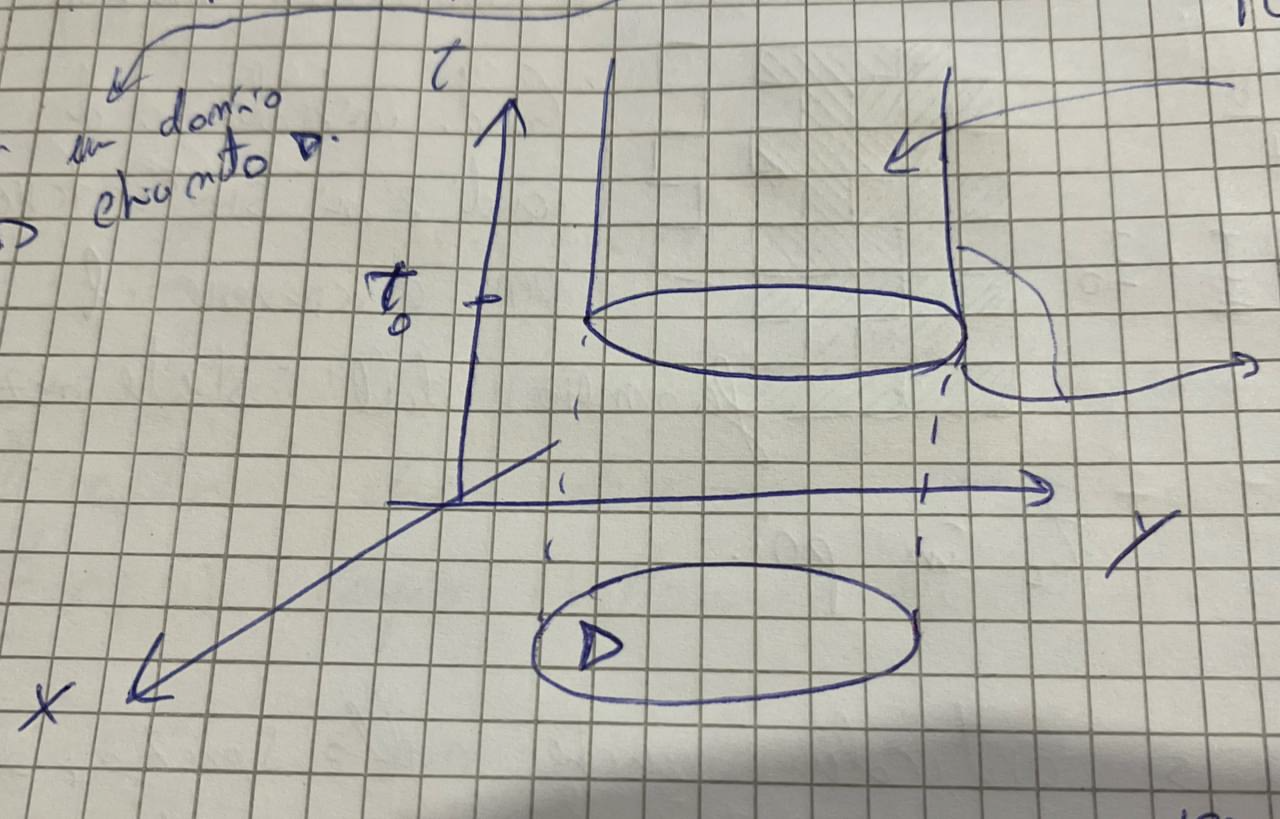
\includegraphics[width=0.5\linewidth]{img/Chapter_one/Chapt1img1.png}
            \caption{"Cilindro spaziotemporale"}
            \label{fig:chapt1img1}
        \end{figure} \\
        Fissato l'istante iniziale $t_{0}$ nel tempo si sviluppa un "cilindro spaziotemporale" all'interno del quale gli eventi (punti dello spazio tempo) relativi al fenomeno elettromagnetico di nostro interesse evolvono. Le sorgenti che influenzano i campi nella regione di spaziotempo interna al cilindro lo fanno passando per i bordi di tale dominio, e dunque vanno viste le condizioni iniziali e al contorno. \\ Le condizioni iniziali per $t_{0}$ devono trovarsi all'interno della base del cilindro e dunque l'unico constraint che hanno è che debbano accadere per $t_{0}$. Viceversa, le condizioni al contorno si trovano sulla superficie laterale del cilindro, libere di cambiare valore nel tempo ma ancorate alle stesse coordinate $(x,y)$ del contorno per ogni istante.\\ \\
        Ci sono 16 incognite per le equazioni di Maxwell, tre per ogni campo vettoriale ed una per $\rho$ che è un campo scalare, ma le equazioni sono otto, in quanto ce ne sono due vettoriali e due scalari. Dobbiamo allora specificare il mezzo all'interno del quale si propaga l'onda. Quese ulteriori relazioni si chiamano \textit{relazioni costitutive dei materiali}. \\ \\
        Quello che abbiamo scritto finora sono le equazioni di Maxwell in forma differenziale e sono equazioni \textit{locali}, cioè il valore dei campi viene calcolato punto per punto istante per istante. Le equazioni differenziali ci piaccino ma richiedono condizioni stringenti, ovvero la derivabilità dei campi ove ne si vuole conoscere il valore puntuale. Allora possiamo scrivere le equazioni in \textit{forma integrale}, che hanno più generalità e permettono di trattare le discontinuità senza problemi. 
        \subsection{Equazioni di Maxwell in forma integrale}
            Le equazioni di Maxwell in forma integrale hanno questa forma qua:
            \begin{align}
                \oint_{C} \underline{e} \cdot \underline{i_{l}} dl = - \frac{\partial}{\partial t}\iint_{S_{C}} \underline{b} \cdot \underline{i_{n}} dS \quad \\
                \oint_{C} \underline{h} \cdot \underline{i_{l}} dl = \frac{\partial}{\partial t} \iint_{S_{C}} \underline{d} \cdot \underline{i_{n}} dS + i(S_{c},t) \\
                \oiint_{\partial V} \underline{d} \cdot \underline{i_{n}} dS = q(V,t) \\
                \oiint_{\partial V} \underline{b} \cdot \underline{i_{n}}dS = 0
            \end{align}
        $C$ è una curva chiusa orientata, cioè esiste un vettore tangente $\underline{i_{l}}$ per cui non ci sono discontinuità nel suo evolvere lungo la curva. $S_{C}$ è la superficie che ha $C$ per bordo e versone normale $\underline{i_{n}}$ punto per punto, che deve essere anch'esso tale da essere continuo nel suo variare lungo la superficie, affinché questa sia orientabile.\\
        I due orientamenti di $C$ ed $S_{C}$ devono essere \textbf{coerenti}, cioè si opera secondo la regola della mano destra: si prende il verso del versore $\underline{i_{l}}$ con tutte le dita tranne il pollice, mentre con quest'ultimo si prende di conseguenza il verso del versore $\underline{i_{n}}$. \\ \\
        La corrente $i(S_{C}, t)$ è per definizione la quantità di carica netta per istante di tempo che passa attraverso la superficie $S_{C}$ in verso concorde alla normale $\underline{i_{n}}$ di tale superficie. Cariche positive con verso concorde alla normale danno contributo positivo, mentre cariche negative con verso concordo alla normale danno contributo negativo e viceversa per versi discordi alla normale. \\ \\
        Nella III e la IV equazione di Maxwell appaiono i flussi di campo di induzione elettrica e magnetica, che per convenzione sono scelti \textbf{uscenti}. Il valore $q(V,t)$ è la quantità di carica all'interno del volume $V$ nell'istante di tempo $t$. \\ \\ 
        Queste equazioni (integrali ndr) non sono locali perché fissato l'istante di tempo bisogna conoscere il valore dei campi su tutte le superfici o curve considerate. Per esempio, per conoscere la quantità di carica $q(V,t)$ all'interno della superficie $V$, bisogna conoscere il valore di $\underline{d}(\underline{r},t)$ su tutta la superficie $\partial V$. \\
        Inoltre, la corrispondenza $(V,t) \to q(V,t)$ non è una funzione numerica, perché $V$ è un volume, cioè un insieme di punti nel piano tridimensionale. Dunque si sta associando un insieme ed un tempo ad un valore $q(V,t)$ relativo ad un insieme ed un tempo. A noi interessa un'espressione numerica e dunque si può pensare di dividere $q(V,t)$ per il volume $V$ in esame e fare il limite, ottenendo la \textbf{densità volumica di carica}:
        \begin{equation}
            \rho(\underline{r},t) = \lim_{V \to 0} \frac{q(V,t)}{\textrm{meas}(V)}
        \end{equation}
        dove $\textrm{meas}(V)$ è la \textit{misura} di $V$, ovvero il valore del volume. La densità volumica è un campo scalare e si misura in $C/m^{3}$. Se ora consideriamo due volumi $V_{1}$ e $V_{2}$, che suppponiamo disgiunti, allora si può affermare:
        \begin{equation}
            q(V_{1} \cup V_{2}, t) = q_{1}(V_{1},t) + q_{2}(V_{2},t) \quad \quad \textrm{se} V_{1} \cap V_{2} = \emptyset
        \end{equation}
        Si può dimostrare che si può passre dalla densità di carica alla carica contenuta in un volume $V$ semplicemente integrando la densità di carica in tutto $V$:
        \begin{equation}
           \label{eqn:integrale_densitaCarica}
            q(V,t) = \iiint_{V} \rho(\underline{r},t)
        \end{equation}
        Il risultato di (\ref{eqn:integrale_densitaCarica}) è intuibile se si considerano tanti piccoli pezzettini disguinti $\Delta V$ così piccoli per i quali il rapporto fra la quantità di carica $dq$ dentro ogni volumetto $\Delta V$ ed il volumetto stesso è praticamente $\rho(\underline{r}, t)$. Dunque sommando tutti questi piccoli contributi e arrivando al limite si ottiene di nuovo la carica totale:
        \begin{equation}
            \frac{dq(\underline{r},t)}{\Delta V} \simeq \rho(\vec{r},t) \implies q \simeq \sum_{i}\Delta V_{i}\rho_{i}(\underline{r},t)
        \end{equation}
        Per la III equazione di Maxwell dividendo ambo membri per la misura di $V$ e facendo il limite:
        \begin{equation}
            \lim_{V \to 0} \frac{1}{\textrm{meas}(V)} \oiint_{\partial V} \underline{d} \cdot \underline{i_{n}} dS = \lim_{V \to 0} \frac{q(V,t)}{\textrm{meas}(V)}
        \end{equation}
        A secondo membro abbiamo la densità di carica mentre al primo abbiamo la definizione della divergeza di $\underline{d}$:
        \begin{equation}
        \label{eqn:def_divergenza}
            \textrm{div}(\underline{d}) = \lim_{V \to 0} \frac{1}{\textrm{meas}(V)} \oiint_{\partial V} \underline{d} \cdot \underline{i_{n}} dS 
        \end{equation}
        che noi scriviamo come prodotto scalare fra l'operatore $\nabla$ e $\underline{d}$. Ricordiamo che $\nabla$ scritto come vettore:
        \begin{equation}
            \nabla = (\frac{\partial }{\partial x}, \frac{\partial }{\partial y}, \frac{\partial }{\partial z})
        \end{equation}
        è puramente rappresentativo perché è un operatore. Con questo arteficio possiamo infatti scrivere:
        \begin{equation}
            \textrm{div}(\underline{d}) = \sum_{i} \frac{\partial}{\partial x_{i}}d_{i}
        \end{equation}
        fermo restando che la definizione della divergenza rimane la (\ref{eqn:def_divergenza}). La divergenza è uno strumento importante che ci permette di studiare la \textit{densità di flusso} in modo puntuale. Lo stesso ragionamento si può effettuare per la IV equazione di Maxwell per ottenere la forma locale.\\ \\
        Consideriamo ora una superficie $\Sigma$. La corrente che passa attraverso $\Sigma$ è definita come:
        \begin{equation}
            \lim_{\Delta t \to 0} \frac{q(\underline{\Sigma}, t + \Delta t)}{\Delta t} = i(\underline{\Sigma}, t)
        \end{equation}
        La corrente così definita non è un concetto puntuale perché perché la dipendenza da $\underline{\Sigma}$ presuppone quella dal \textit{versore} normale a $\Sigma$. \\
        Per capire meglio questa cosa ed in che modo è un problema, definiamo la densità di corrente:
        \begin{equation}
            \underline{j}(\underline{r}, t) = \lim_{\Sigma \to 0} \frac{i(\underline{\Sigma},t)}{\textrm{meas}(\Sigma)}
        \end{equation}
        Questa definizione non è completa, perché bisogna tener conto della dipendenza dall'orientamento della normale nel punto nel quale è collassata la superficie $\Sigma$, ergo bisogna più correttamente scrivere:
        \begin{equation}
            \underline{j}_{n}(\underline{r},t)
        \end{equation}
        Si ottiene l'espressione di un campo solo quando si specifica la normale $\underline{i}_{n}$, ottenendo dunque per ogni punto infiniti possibili campi (per ogni singola normale che si può prendere a partire da un punto). Questa è male perché a noi interessa l'espressione di un campo, cioè un oggetto per il quale date le coordinate spaziotemporale (ovvero quattro numeri) si ottiene un'altra grandezza. \\
        Abbiamo scritto $\underline{j}_{n}$ con la notazione utilizzata per i campi vettoriali, dunque vediamo come ci si arriva. Consideriamo un tetraedro nel piano tridimensionale $Oxyz$.
        \begin{figure}[h!]
            \centering
            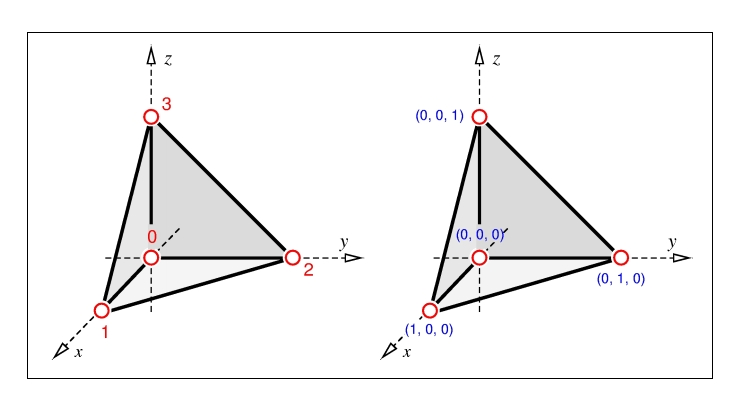
\includegraphics[width=0.75\linewidth]{img//Chapter_one/Chapt1img2.png}
            \caption{Immagine a puro scopo illustrativo}
        \end{figure}
        Assumiamo per ora valido il principio di conservazione per la carica (vedremo più avanti in che modo questo viene incluso nelle equazioni di Maxwell). Considerato un volume $V$ contenente carica $q(V,t)$ all'istante di tempo $t$, vale:
        \begin{equation}
        \label{eqn:conservazione_carica}
            \frac{\partial}{\partial t}q(V,t) = - i(\partial \underline{V},t)
        \end{equation}
        Questa relazione è inutitiva se si pensa, per esempio, a della carica negativa uscente. Questo implica che la derivata è positiva (perché carica negativa uscente = carica positiva entrante) ma carica negativa concorde al verso della normale implica corrente negativa, relazione verificata dalla (\ref{eqn:conservazione_carica}). \\
        Se chiamiamo i versori delle tre facce giacenti sui piani $\Sigma_{x}, \Sigma_{y}, \Sigma_{z}$ e quello della faccia "obliqua" $\Sigma_{n}$, non è difficile vedere che $\Sigma_{x}$ è normale al piano $yz$ e così via per $\Sigma_{y}$ e $\Sigma_{z}$. Allora scegliendo i versori $\Sigma_{i}$ ($i \in [x,y,z]$) concordi a quelli degli assi, questi risultano entranti nel tetraedro. Scegliamo, per convenzione, $\Sigma_{n}$ uscente dalla faccia obliqua. In condizioni stazionarie le derivate si annullano, risultato matematico che corrisponde nel nostro caso a carica netta entrante nel tetraedro pari a zero. Alla luce di ciò possiamo scrivere:
        \begin{equation}
            0 = i(\partial \underline{V}, t) = i(\underline{\Sigma}_{n}, t)+i(\underline{-\Sigma}_{x},t)+i(\underline{-\Sigma}_{y},t)+i(\underline{-\Sigma}_{z},t) = 0
        \end{equation}
        da cui si ottiene, intuitivamente, che il flusso di corrente entrante per le tre facce giacenti sui piani generati dai tre assi è pari a quello uscente dalla quarta superficie:
        \begin{equation}
            i(\underline{\Sigma}_{n}, t) = \sum_{k} i(\underline{\Sigma}_{k}, t) \qquad \qquad k \in (x,y,z)
        \end{equation}
        Scriviamo allora l'espressione in questo modo:
        \begin{equation}
            \frac{i(\underline{\Sigma}, t)}{\textrm{meas}(\underline{\Sigma}_{n})} = \sum_{k} \frac{i(\underline{\Sigma_{k}},t)}{\textrm{meas}(\Sigma_{k})} \frac{\textrm{meas}(\Sigma_{k})}{\textrm{meas}(\Sigma_{n})}
        \end{equation}
        dove $k \in (x,y,z)$. Facendo collassare il volume al punto (che poi corrisponde all'origine del nostro sistema di riferimento) si ottiene:
        \begin{align}
            \frac{i(\underline{\Sigma_{n}})}{\textrm{meas}(\Sigma_{n})} \to j_{n}(\underline{r},t) \\
            \frac{i(\underline{\Sigma_{k}})}{\textrm{meas}(\Sigma_{k})} \to j_{k}(\underline{r},t) \qquad \forall k
        \end{align}
        Il problema ora è vedere come collassa il rapporto:
        \begin{equation}
            \frac{\textrm{meas}(\Sigma_{k})}{\textrm{meas}(\Sigma_{n})}
        \end{equation}
        Se consideriamo il collasso bidimensionale del tetraedro su una delle facce, per esempio $x$, lavoriamo con il triangolo:
        \begin{figure}[h!]
            \centering
            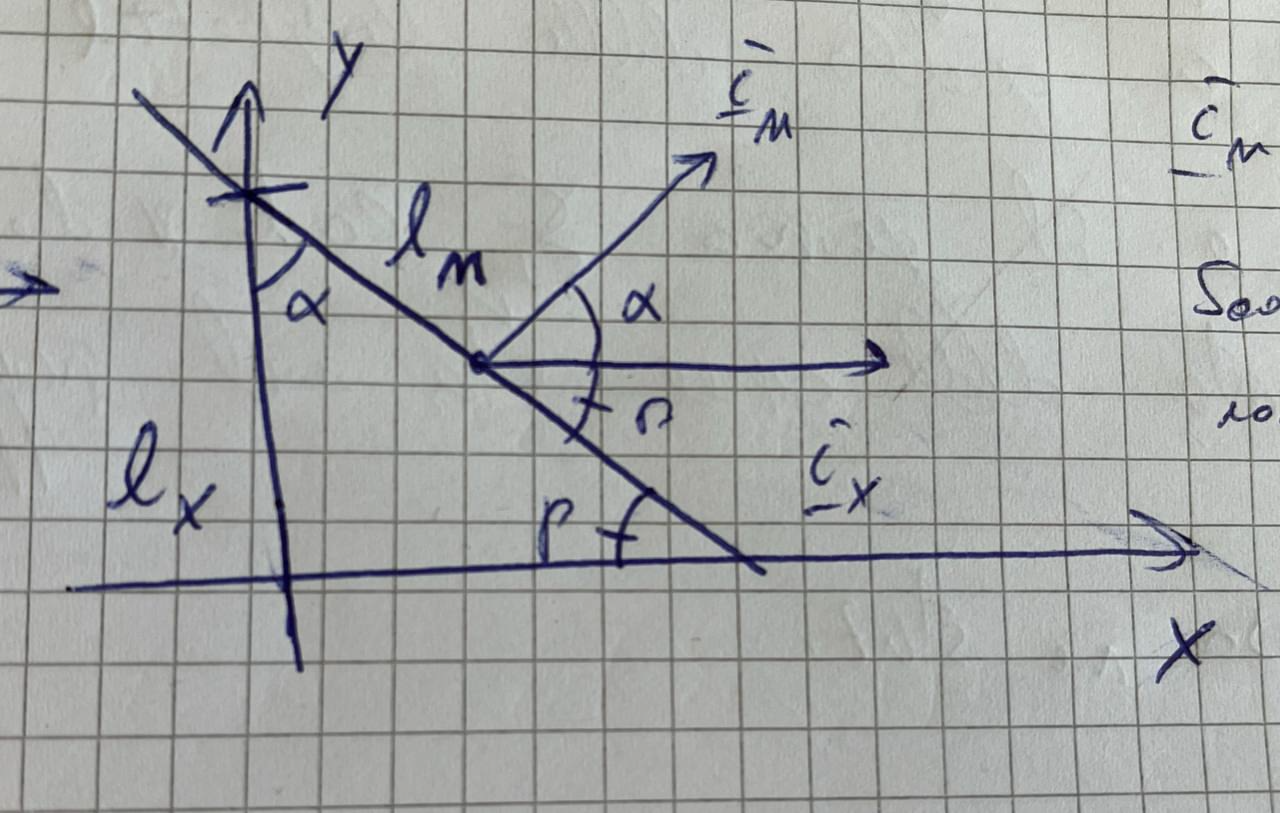
\includegraphics[width=0.75\linewidth]{img//Chapter_one/chap1img3.png}
            \caption{}
        \end{figure}
        La normale $\underline{i}_{n}$ alla superficie $\Sigma_{z}$ e quella $\underline{i}_{x}$ alla superficie $\Sigma_{x}$ formano un angolo $\alpha$ pari a quello formato dalle rette giacenti sulle due superfici. Dal momento che il rapporto fra le aree dei due triangoli (nel disegno 3D) corrispondenti alle facce $\Sigma_{x}$ e $\Sigma_{n}$ si riduce al rapporto fra le altezze (in quanto suddetti triangoli condividono la base), allora si può scrivere:
        \begin{equation}
            \frac{\textrm{mis}(\Sigma_{x})}{\textrm{mis}(\Sigma_{n})} = \frac{l_{x}}{l_{n}} = \cos{(\alpha)} = \underline{i}_{n} \cdot \underline{i}_{x}
        \end{equation}
        L'ultimo passaggio è giustificato dalla definizione di prodotto scalare fra due vettori e tenendo conto che i versori hanno modulo unitario.\\
        A valle di ciò che abbiamo detto possiamo scrivere la stessa cosa per le altre due dimensioni ed ottenere:
        \begin{equation}
            j_{n}(\underline{r},t) = j_{x}(\underline{r},t)(\underline{i}_{x}\cdot \underline{i}_{n})+j_{x}(\underline{r},t)(\underline{i}_{y}\cdot \underline{i}_{y})+j_{z}(\underline{r},t)(\underline{i}_{z}\cdot \underline{i}_{n})
        \end{equation}
        che riscriviamo come:
        \begin{equation}
            j_{n}(\underline{r},t) = (j_{x}\underline{i}_{x}+j_{y}\underline{i}_{y}+j_{z}\underline{i}_{z}) \cdot \underline{i}_{n} = \underline{j}(\underline{r},t) \cdot \underline{i}_{n}
        \end{equation}
        dove $\underline{j}(\underline{r},t)$ è il vettore densità di corrente. Dunque è possibile ottenere la densità di corrente relativa ad una superficie tramite il prodotto scalare fra il vettore densità di corrente ed il versore normale alla superficie stessa.\\
        Ovviamente è possibile tornare indietro:
        \begin{equation}
            i(\underline{\Sigma}, t) = \iint_{\Sigma} \underline{j} (\underline{r},t) \cdot \underline{i}_{n} d \Sigma
         \end{equation}
         Nel caso non stazionario valgono le stesse relazioni che abbiamo appena trovato. Dimostriamolo considerando l'espressione che tiene conto delle derivate non nulle:
         \begin{equation}
             i(\underline{\Sigma}_{n}, t) = \sum_{k} i(\underline{\Sigma}_{k},t) - \frac{\partial}{\partial t}q
         \end{equation}
         che sotto l'ipotesi di poter passare le derivate sotto il segno d'integrale scriviamo nella forma più comoda:
         \begin{equation}
             i(\underline{\Sigma}_{n}, t) = \sum_{k} i(\underline{\Sigma}_{k},t) - \iiint_{V} \frac{\partial}{\partial t}\rho
         \end{equation}
        Come in precedenza, possiamo dividere ambo membri per $\textrm{meas}(\Sigma_{n})$, ma dobbiamo capire dove converge il rapporto:
        \begin{equation}
            \frac{\displaystyle\iiint_{V} \frac{\partial}{\partial t}\rho}{\textrm{meas}(\Sigma_{n})}
        \end{equation}
        Per il teorema della media esiste un $\rho_{0}$ tale per cui:
        \begin{equation}
            \iint_{V} \frac{\partial}{\partial t} \rho dV = \frac{\partial \rho}{\partial t} |_{\rho = \rho_{0}} \cdot \textrm{meas}(V)
        \end{equation}
        Poiché $\textrm{meas}(V)$ va a zero più velocemente di $\textrm{meas}(\Sigma_{n})$, cioè è un infinitesimo di ordine superiore rispetto a $\textrm{meas}(\Sigma_{n})$, allora il contributo associato alla variazione della carica interna al volume è nullo, ragion per la quale quanto detto per il caso stazionario vale anche nel caso non stazionario. \\ \\
        Ora che abbiamo capito perché la corrente, che è una quantità scalare, ha come densità una quantità vettoriale, consideriamo la II° equazione di Maxwell\footnote{Qui andrebbe scritto a secondo membro il contributo della densità di corrente come $\iint_{S_{C}} \underline{j} \cdot \underline{i}_{n}dS$, ma la dipendenza della corrente dalla superficie considerata è contenuta nella dipendenza di questa dal proprio versore, che quindi viene esplicitato quando si scrive la corrente come flusso della densità di corrente}:
        \begin{equation}
            \oint_{C} \underline{h} \cdot \underline{i}_{l} dl = \frac{\partial}{\partial t} \iint_{S_{C}} \underline{d} \cdot \underline{i}_{n}dS + \frac{\partial}{\partial t} \iint_{S_{C}} i(\underline{S}_{C}, t)dS
        \end{equation}
        
        Per arrivare ad esplicitare la forma locale della II° legge, consideriamo tre casi elementari sui quali si possono costruire quelli più complessi, ovvero l'applicazione della legge su piani con normali corrispondenti ai tre assi di riferimento. Esaminiamo il caso di una superficie piana $S_{C_{x}}$ con contorno $C_{x}$ e normale $\underline{i}_{x}$. Gli altri due casi con $\underline{i}_{y}$ ed $\underline{i}_{z}$ si ricavano in modo analogo. 
        \begin{figure}[h!]
            \centering
            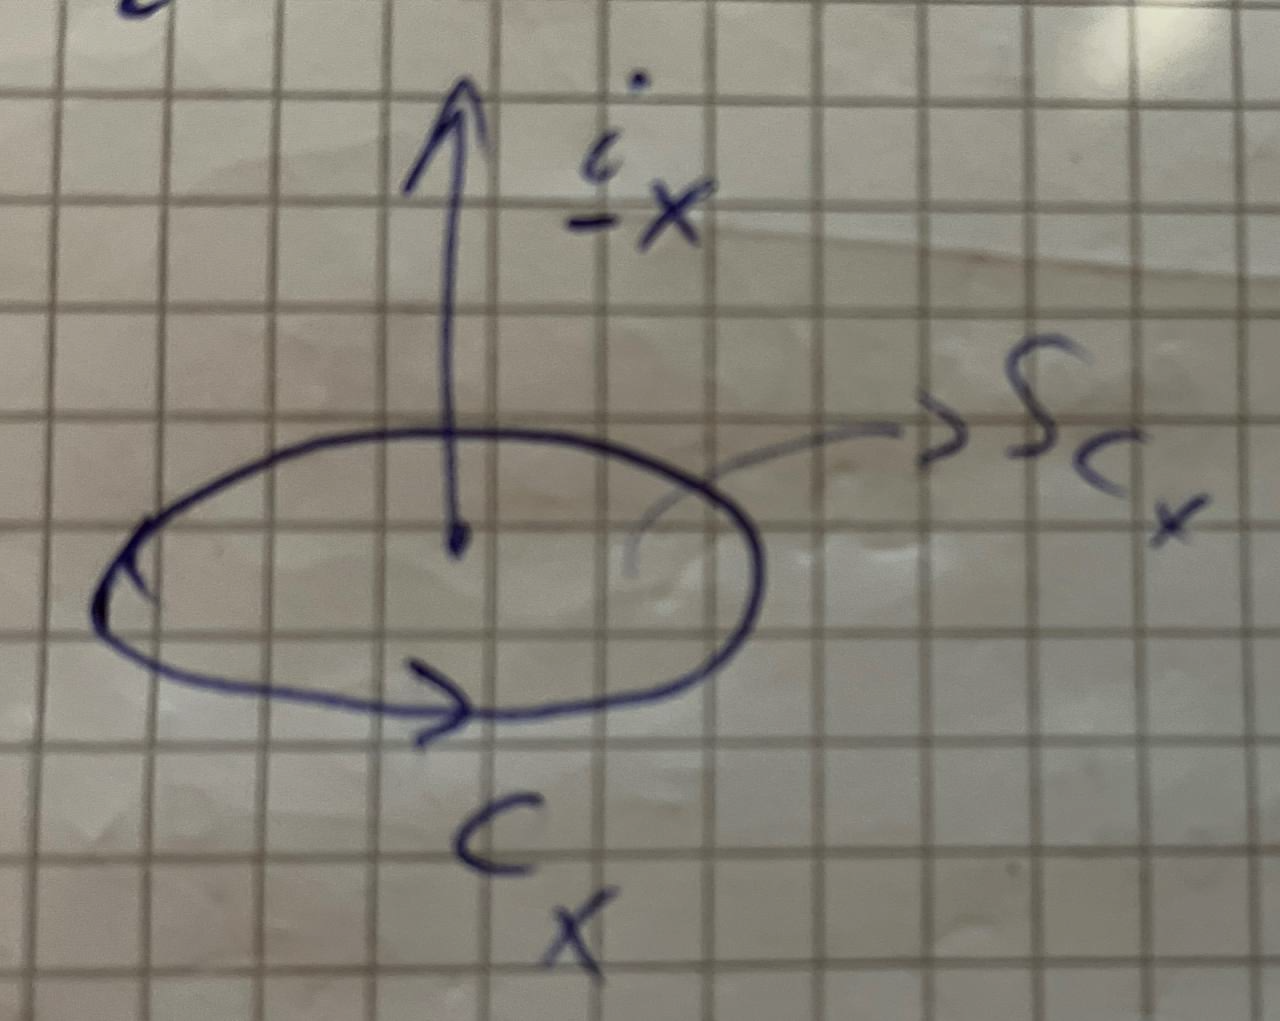
\includegraphics[width=0.35\linewidth]{img//Chapter_one/Chapt1img4age.png}
            \caption{}
        \end{figure}
        Dividiamo per $\textrm{meas}(S_{C_{x}})$
        \begin{equation}
            \frac{\displaystyle \oint_{C_{x}} \underline{h} \cdot \underline{i}_{l}dl}{\textrm{meas}(S_{C_{x}})} = \frac{\partial}{\partial t} \frac{\displaystyle \iint_{S_{C_{c}}} \underline{d} \cdot \underline{i}_{n}dS}{\textrm{meas}(S_{C_{x}})} + \frac{\partial}{\partial t} \frac{i(\underline{S_{c}}, t)}{\textrm{meas}(S_{C_{x}})}
        \end{equation}
        Facendo collassare la superficie ad un punto otteniamo la densità di corrente al secondo pezzo del membro di destra, mentre il primo termine di destra lo scriviamo come:
        \begin{equation}
            \frac{\partial}{\partial t} \frac{\displaystyle \iint_{S_{C_{x}}} \underline{d} \cdot \underline{i}_{n} dS}{\textrm{meas}(S_{C_{x}})} = \frac{\displaystyle  \iint_{S_{C_{x}}} \frac{\partial}{\partial t} \underline{d} \cdot \underline{i}_{n} dS}{\textrm{meas}(S_{C_{x}})}  
        \end{equation}
        sotto l'ipotesi che si possa passare la derivata sotto il segno di integrale. Nel nostro caso $\underline{i}_{n} = \underline{i}_{x}$ e dunque moltiplicare $\underline{d}$ per $\underline{i}_{x}$ equivale a prelevare la componente di $\underline{d}$ lungo $x$:
        \begin{equation}
            \frac{\displaystyle  \iint_{S_{C_{x}}} \frac{\partial}{\partial t} d_{x} \ dS}{\textrm{meas}(S_{C_{x}})}  
        \end{equation}
        Per il teorema della media questa quantità è pari a:
        \begin{equation}
            \frac{\partial}{\partial t}|_{x=x_{0}} \frac{\textrm{meas}(S_{C_{x}})}{\textrm{meas}(S_{C_{x}})} = \frac{\partial}{\partial t} d_{x}|_{x=x_{0}}
        \end{equation}
        dove $x_{0}$ è il punto nel quale la superficie collassa. \\
        Introduciamo a questo punto il \textbf{rotore} come \textit{densità di circuitazione} per esprimere la quantità del membro di sinistra. La componente lungo $x$ del rotore è definita come:
        \begin{equation}
            \textrm{rot}_{x}(\underline{h}) = \lim_{S_{C_{x}} \to x_{0}} \frac{\displaystyle \oint \underline{h} \cdot \underline{i}_{x} dl}{\textrm{meas}(S_{C_{x}})}
        \end{equation}
        Di nuovo, il gradiente si può esprimere in modo simbolico come abbiamo fatto con la divergenza come:
        \begin{equation}
            \textrm{rot}(\underline{h}) = \nabla \times \underline{h} = \begin{vmatrix} i_{x} & i_{y} & i_{z} \\ \frac{\partial}{\partial_{x}} & \frac{\partial}{\partial_{y}} & \frac{\partial}{\partial_{z}}  \\ h_{x} & h_{y} & h_{z} \end{vmatrix}
        \end{equation}
        Per le altre due componenti del rotore la definizione è analoga, basta fare il prodotto scalare con i versori $\underline{i}_{y}$ e $\underline{i}_{z}$. Si può tornare indietro integrando:
        \begin{equation}
            \oint_{C_{x}} \underline{h} \cdot \underline{i}_{x} dl = \iint_{S_{C_{x}}} \nabla \times \underline{h} \cdot \underline{i}_{x} dS
        \end{equation}
        che esteso alle tre dimensioni non è nient'altro che il teorema di Stokes\footnote{"The line integral of a vector field over a loop is equal to the surface integral of its curl over the enclosed surface."}
        \\
        In definitiva otteniamo:
        \begin{equation}
            \iint_{S_{C}} \nabla \times \underline{h} \cdot \underline{i}_{n} dS = \frac{\partial}{\partial t} \iint_{S_{C}} \underline{d} \cdot \underline{i}_{n} dS + \iint_{S_{C}} \underline{j} \cdot \underline{i}_{n} dS
        \end{equation}
        Ottenendo, eguagliando gli integrandi (il dominio di integrazione ora è lo stesso) l'equazione in forma locale:
        \begin{equation}
            \nabla \times \underline{h} = \frac{\partial}{\partial t} \underline{d} + \underline{j}
        \end{equation}
        Ugualmente si ricava la prima equazione di Maxwell in forma locale:
        \begin{equation}
            \nabla \times \underline{e} = - \frac{\partial}{\partial t} \underline{b}
        \end{equation}
        Dobbiamo ora capire come fare in presenza di discontinuità del campo EM. Consideriamo la quarta equazione di Maxwell:
        \begin{equation}
            \oiint_{\partial V} \underline{b} \cdot \underline{i}_{n} dS =0 \ \ \textrm{oppure in forma locale} \ \ \nabla \cdot \underline{b} = 0
        \end{equation} \newpage
        \section{Equazioni di raccordo}
        \subsection{Quarta e terza legge di Maxwell}
        Consideriamo allora una superficie $\Sigma$\footnote{$\Sigma$ potrebbe essere una superficie di divisione fra due mezzi ove il campo cambia bruscamente a causa dell'altrettanto brusco cambio di materiale nel quale si propaga} ove ci potrebbero essere delle discontinuità:
        \begin{figure}[h!]
            \centering
            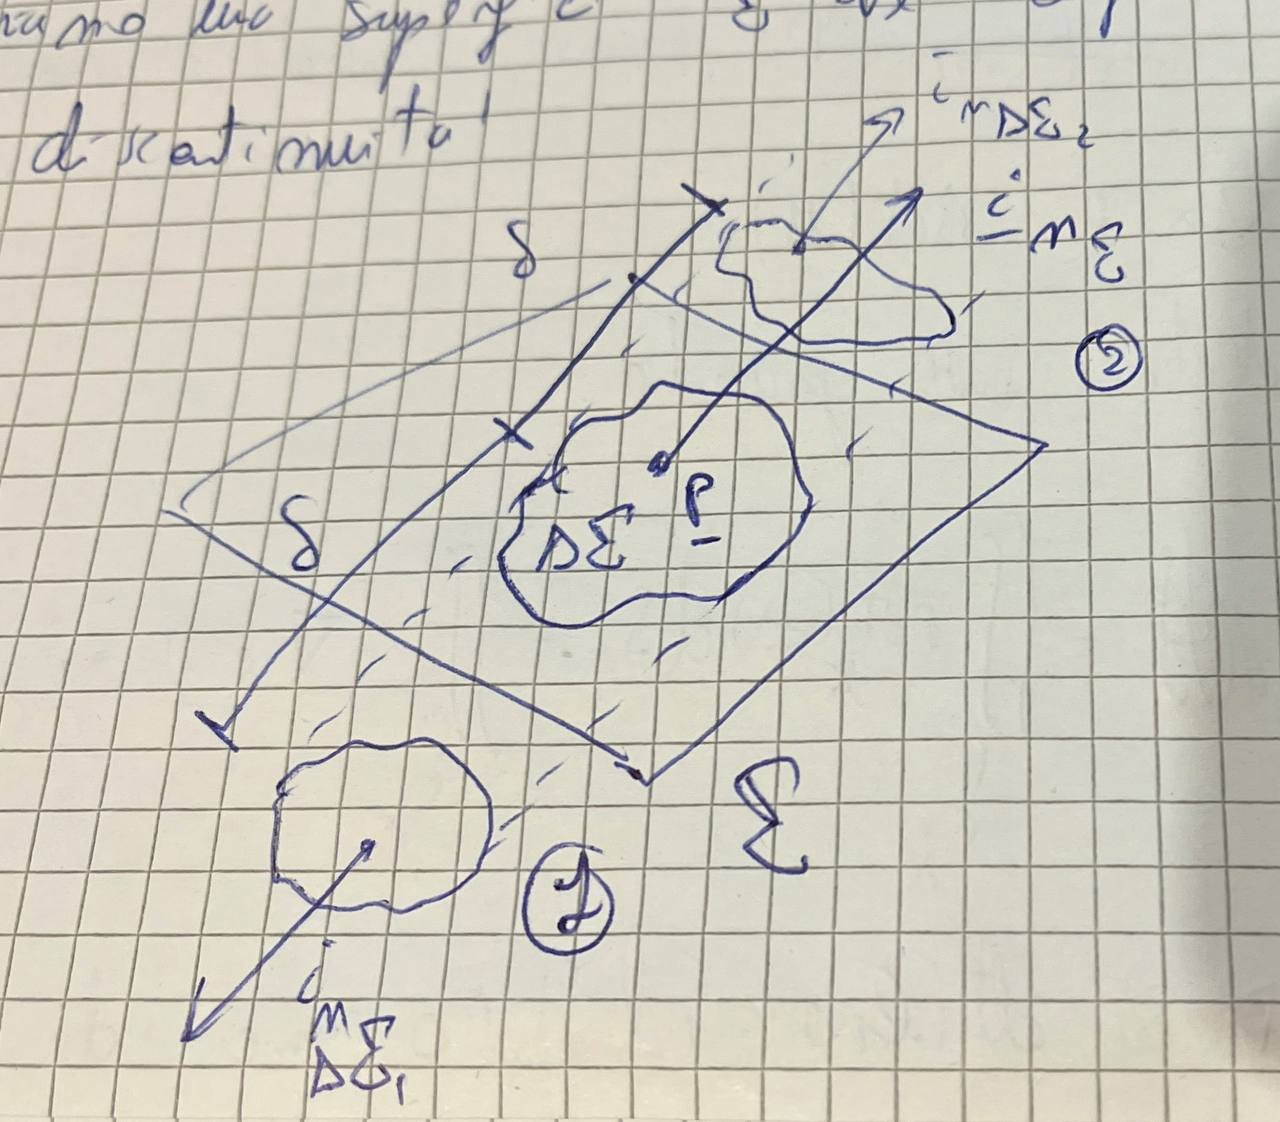
\includegraphics[width=0.5\linewidth]{img//Chapter_one/Chapt1img5.png}
            \caption{}
        \end{figure}
        Sulla $\Sigma$ consideriamo una superficie infinitesima $\Delta \Sigma$ e la facciamo traslare lungo la direzione della normale in entrambi i versi di una quantità $\delta$, generando il cilindroide di volume $V$, altezza $2 \delta$ e basi $\Delta \Sigma$. Chiamiamo la zona al di sotto della superficie "1" con la relativa base $\Delta \Sigma_{1}$ e normale opposta a quella di $\Delta \Sigma$, mentre quella di sopra sarà la superficie "2" con relativa base $\Delta \Sigma_{2}$ e normale con verso concorde a quella di $\Delta \Sigma$. La superficie laterale è $\Delta \Sigma_{l}$. \\ \\
        L'integrale di flusso attraverso il cilindroide si può scrivere come somma di tre contributi \footnote{Notare che non sono integrali chiusi perché tutti e tre formano una superficie chiusa, ma da soli sono semplicemente integrali di superfici aperte}:
        \begin{equation}
            \oiint_{\partial V} \underline{b} \cdot \underline{i_{n}} = \iint_{\Delta \Sigma_{1}} \underline{b} \cdot \underline{i}_{n} + \iint_{\Delta \Sigma_{2}} \underline{b} \cdot \underline{i}_{n} + \iint_{\Delta \Sigma_{1}} \underline{b} \cdot \underline{i}_{l}
        \end{equation} \\
        Dobbiamo far collassare il cilindroide al punto $P$. Facciamo il limite per $\delta \to 0$ ed analizziamo separatamente i tre contributi. Per la superficie laterale, la quantità:
        \begin{equation}
            \lim_{\delta \to 0} \iint_{\Delta \Sigma_{l}} \underline{b} \cdot \underline{i}_{n} dS
        \end{equation}
        \\ tende alla curva corrispondente al bordo di $\Delta \Sigma$. Per l'assoluta continuità dell'integrale\footnote{Integrando una funzione in un dominio perdendo un dimensione e tale funzione è regolare allora l'integrale va a zero} il contributo della superficie laterale è nullo. \\
        Per la superficie $\Delta \Sigma_{1}$, questa converge alla superficie $\Delta \Sigma$ come insieme di punti ma con normale opposta a quella di quest'ultima, dunque:
        \begin{equation}
            \iint_{\Delta \Sigma_{1}} \underline{b} \cdot \underline{i}_{n_{\Sigma}} dS \stackrel{\delta \to 0}{\to}  \iint_{\Delta \Sigma} \underline{b} \cdot (- \underline{i}_{n_{\Sigma}} )dS
        \end{equation} \\
        In modo analogo, $\Delta\Sigma_{2} \stackrel{ \delta \to 0}{\to} \Delta \Sigma$ ottenendo:
        \begin{equation}
            \iint_{\Delta \Sigma_{2}} \underline{b} \cdot \underline{i}_{n_{\Sigma}} dS \stackrel{\delta \to 0}{\to}  \iint_{\Delta \Sigma} \underline{b} \cdot - \underline{i}_{n_{\Sigma}} dS
        \end{equation}
        Tenendo conto del fatto che il campo $\underline{b}$ avrà espressioni generalmente diverse in "1" e "2", ovvero $\underline{b}_{1}$ e $\underline{b}_{2}$, scriviamo in definitiva:
        \begin{equation}
            \lim_{\delta \to 0} \iint_{\Delta \Sigma_{1}} \underline{b} \cdot \underline{i}_{n} + \iint_{\Delta \Sigma_{2}} \underline{b} \cdot \underline{i}_{n} + \iint_{\Delta \Sigma_{1}} \underline{b} \cdot \underline{i}_{l} = \iint_{\Delta \Sigma} (\underline{b}_{2}-\underline{b}_{1}) \cdot \underline{i}_{n}dS = 0
        \end{equation}
        Possiamo affermare che l'argomento di quest'integrale è nullo grazie al \textbf{teorema della localizzazione}, il quale afferma che se una funzione $f(x)$ viene integrata su un dominio $I$ arbitrario e per ogni $I$ il suo integrale ha valore nullo, allora $f(x) = 0$ quasi ovunque. \\
        Nel nostro caso $\Delta \Sigma$ è stata scelta in modo arbitrario e dunque possiamo scrivere:
        \begin{equation}
        \label{eqn:condizione_raccordo4}
            (\underline{b}_{2}-\underline{b}_{1}) \cdot \underline{i}_{n_{\Sigma}} = 0 \quad \quad \forall \Delta \Sigma
        \end{equation}
        La (\ref{eqn:condizione_raccordo4}) è la \textit{quarta equazione di raccordo} che va utilizzata in presenza di discontinuità per le quali non è possibile utilizzare la quarta legge di Maxwell in forma locale. È importante notare come la (\ref{eqn:condizione_raccordo4}) derivi direttamente dalle equazioni di Maxwell e sottolinea come esse debbano valere anche in presenza di discontinuità. In questo caso, la legge che abbiamo appena ricavato richiede che le componenti normali\footnote{sono infatte moltiplicate per il versore normale} del campo di induzione magnetica $\underline{b}$ si conservino. \\
        Un ultima osservazione va fatta sulla drammatica differenza di significato fra le condizioni al \textit{contorno} e quelle di \textit{raccordo}: le prime danno un'informazione numerica, cioè quanto devono valere i campi alla frontiera, mentre quelle di raccordo danno informazioni circa la relazione fra i campi delle due superfici, come nel caso appena trattato fra $\underline{b}_{1}$ e $\underline{b}_{2}$. \\ \\
        Passiamo ora alla terza equazion di raccordo. Utilizziamo la stessa figura di prima ma stavolta l'equazione da considerare è:
        \begin{equation}
            \oiint_{\partial V} \underline{d} \cdot \underline{i}_{n} dS = q(V, t)
        \end{equation}
        che è più complessa rispetto alla quarta per la presenza di un termine non per forza nullo a secondo membro. \newpage Come prima scriviamo:
        \begin{equation}
            \iint_{\Delta \Sigma_{1}} \underline{d} \cdot \underline{i}_{n} dS + \iint_{\Delta \Sigma_{2}} \underline{d} \cdot \underline{i}_{n} dS + \iint_{\Delta \Sigma_{l}} \underline{d} \cdot \underline{i}_{n}  dS= q(V,t) 
        \end{equation}
        I termini del primo membro con lo stesso procedimento di prima danno, al limite per $\delta \to 0$:
        \begin{equation}
            \iint_{\Delta \Sigma} (\underline{e}_{2}-\underline{e}_{1}) \cdot \underline{i}_{n} dS
        \end{equation}
        ma dove converge $\displaystyle \lim_{\delta \to 0} q(V,t)$? Consideriamo una superficie $\Sigma$ con della carica distribuita su uno strato di un certo spessore:
        \begin{figure}[h!]
            \centering
            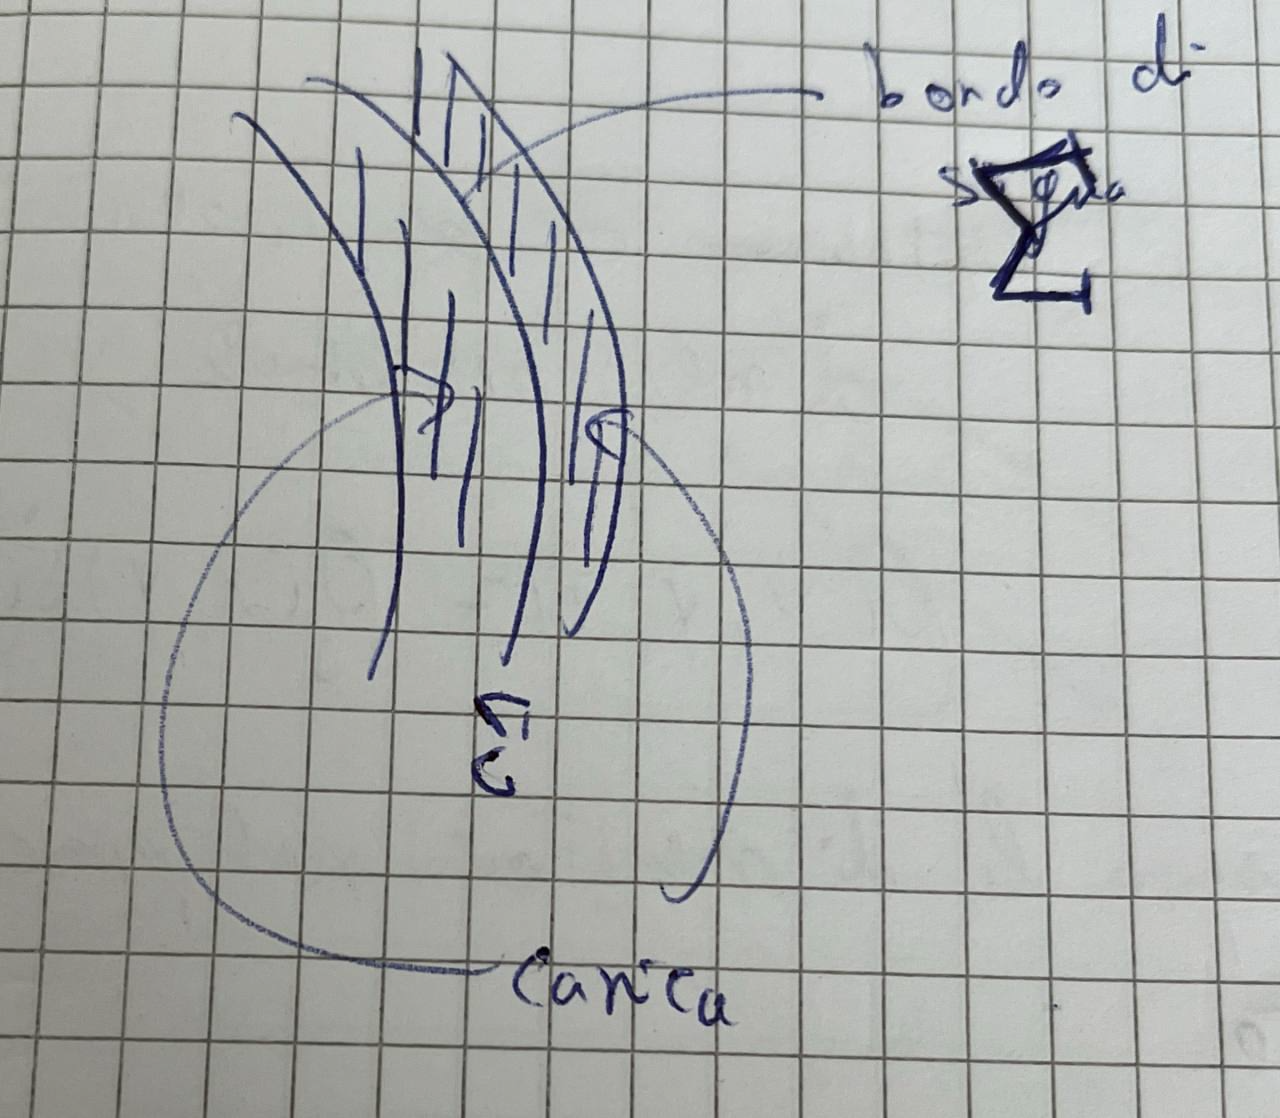
\includegraphics[width=0.5\linewidth]{img//Chapter_one/chapt1img6.png}
            \caption{}
        \end{figure}
        Se tale spessore è trascurabile rispetto alle altre dimensioni in gioco, possiamo dire in modo approssimato che la carica ivi contenuta sia totalmente sulla superficie $\Sigma$, cioè stiamo passando da una densità di carica volumica ad una superficiale. Teniamo conto infatti che:
        \begin{equation}
            q(V,t) = \iiint_{V} \rho dV
        \end{equation}
        Ma se la densità $\rho(x,y,z)$ è distribuita su una superficie\footnote{che supponiamo piana perché tutte le superfici se non le vedi come un nerd sono piane}, allora deve essere non nulla soltanto in quei punti che hanno come coordinata la $z_{0}$ fissata del piano:
        \begin{figure}[h!]
            \centering
            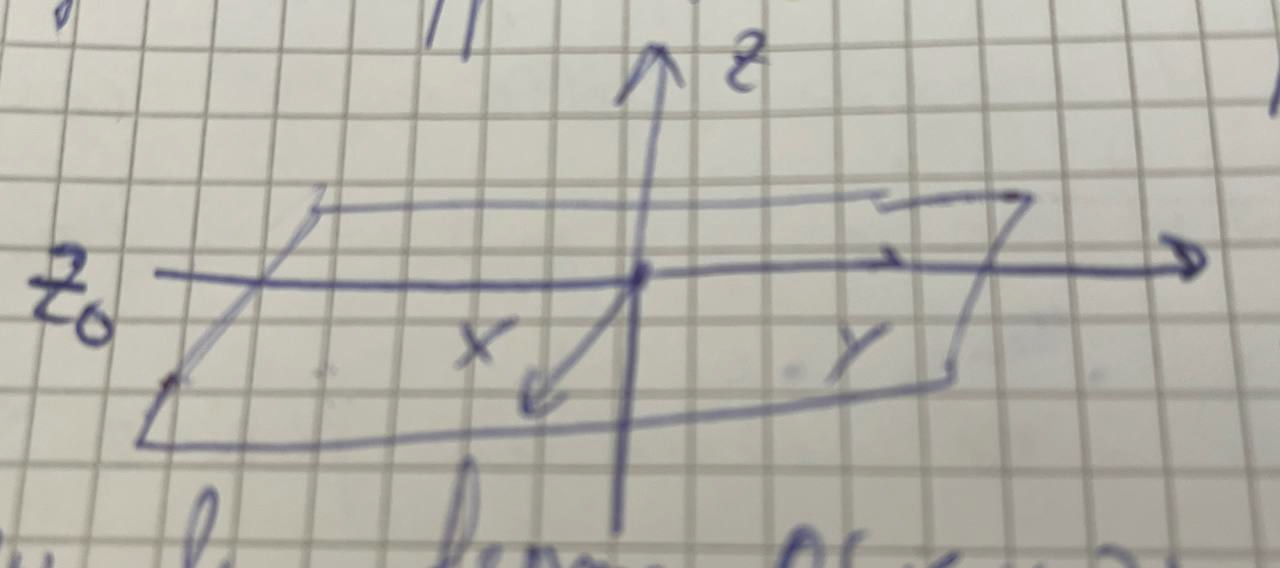
\includegraphics[width=0.36\linewidth]{img/Chapter_one/chapt1img7.png}
            \caption{}
        \end{figure}
        \newpage
        allora $\rho(x,y,z)$ dovrà avere una forma del genere:
        \begin{equation}
        \label{eqn:densità_carica_sup}
            \rho (x,y,z) = \rho_{S}(x,y)\delta(z)
        \end{equation}
        dove $\rho_{S}(x,y)$ è la \textbf{densità superficiale di carica} che ha dimensioni $C/m^{2}$. È bene notare che affinché la (\ref{eqn:densità_carica_sup}) abbia dimensionalmente senso, la $\delta(z)$ deve avere le dimensioni di un inverso di una lunghezza. La delta infatti è tale per cui:
        \begin{equation}
            \int ^{\chi} _{-\chi} \delta(\chi) d\chi = 1
        \end{equation}
        qualunque sia $\chi$. Poiché il risultato è un numero adimensionale, la delta deve avere le dimensioni inverse di $\Delta \chi$. Nel nostro caso, l'integrale fatto lungo la componente $z$, che ha le dimensioni di una lunghezza, deve ritornare $1$ per la proprietà di $\delta (z)$, che quindi è omogenea ad $\displaystyle \frac{1}{m}$.
        In definitiva, possiamo scrivere:
        \begin{equation}
            \iint_{\Delta \Sigma} [(\underline{d}_{2}-\underline{d}_{1}) \cdot \underline{i}_{n} -\rho_{s}]dS = 0
        \end{equation}
        Applicando come prima il teorema della localizzazione otteniamo la \textit{terza equazione al raccordo}:
        \begin{equation}
        \label{eqn:cond_raccordo_3}
            (\underline{d}_{2}-\underline{d}_{1}) \cdot \underline{i}_{n} = \rho_{s}
        \end{equation} \\
        La (\ref{eqn:cond_raccordo_3}) asserisce che la componete normale del campo di induzione magnetica nel passaggio da un mezzo all'altro, in presenza di accumuli di carica superficiali con densità di carica $\rho_{s}$, debbano variare proprio di $\rho_{s}$.
        \newpage
        \subsection{Seconda e prima legge di Maxwell}
        Passiamo ora alla II equazione di Maxwell.
        \begin{figure}[h!]
            \centering
            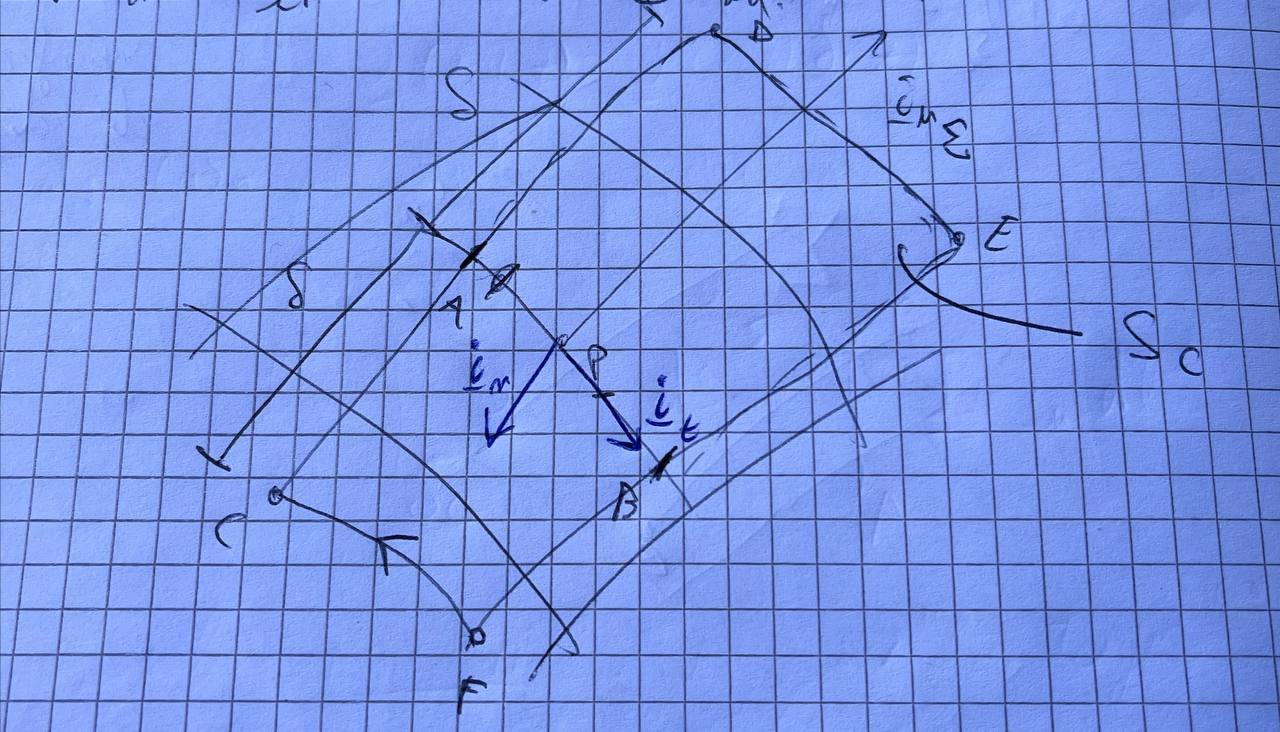
\includegraphics[width=0.75\linewidth]{img//Chapter_one/chapt1img5age.png}
            \caption{}
        \end{figure}
        Consideriamo una superficie $\Sigma$ e scegliamo arbitrariamente uno del fascio di piani generato dalla normale a $\Sigma$. Tale piano individua sulla superficie $\Sigma$ la curva $AB$. A partire da AB efiniamo il rettangoloide $CDEF$ dove $DE$ e $CF$ sono distanti $\delta$ rispetto ad $AB$. Orientiamo la curva $CFDE$, che chiamiano $\mathcal{C}$ con tangente $\underline{i}_{t}$, la quale è il bordo della superficie $S_{\mathcal{C}}$ con normale $\underline{i}_{n}$, corrispondente proprio al rettangoloide individuato da $CDEF$. \\
        La circuitazione lungo $\mathcal{C}$ può essere scritta come:
        \begin{equation}
            \oint_{\mathcal C} \underline{h} \cdot \underline{i}_{l} dl = \int_{C} ^{D} \underline{h} \cdot \underline{i}_{l}dl + \int_{D} ^{E} \underline{h} \cdot \underline{i}_{l}dl +\int_{E} ^{F} \underline{h} \cdot \underline{i}_{l}dl +\int_{C} ^{F} \underline{h} \cdot \underline{i}_{l}dl  
        \end{equation}
        Vediamo dove convergono questi termini per $\delta \to 0$. L'integrale di linea lungo $DC$ va a zero, perché perde una dimensione\footnote{in quanto $DC$ sta collassando al punto $A$}. Lo stesso discorso va fatto per quello lungo $EF$.\\
        Per $\delta \to 0$ la curva $DE$ diventa pari ad $AB$ con versore concorde\footnote{orientando la curva in senso orario} a quello tangente ad essa. Il campo nella zona superiore, dove c'è $DE$ per intenderci, ha valore $\underline{h}_{2}$ e quindi:
        \begin{equation}
            \int_{D} ^{E} \underline{h} \cdot \underline{i}_{l}dl \stackrel{\delta \to 0}{\to} \int_{A} ^{B} \underline{h}_{2} \cdot \underline{i}_{t} dl
        \end{equation}
        In modo analogo:
        \begin{equation}
            \int_{C} ^{F} \underline{h} \cdot \underline{i}_{l}dl \stackrel{\delta \to 0}{\to} \int_{A} ^{B} \underline{h}_{1} \cdot (-\underline{i}_{t}) dl
        \end{equation}
        \\ A secondo membro, il contributo associato al campo induzione elettrica è:
        \begin{equation}
            \lim_{\delta \to 0} \frac{\partial}{ \partial t} \iint_{S_{\mathcal{C}}} \underline{d} \cdot \underline{i}_{n}dS = \lim_{\delta \to 0} \iint_{S_{\mathcal{C}}} \frac{\partial}{\partial t} \underline{d} \cdot \underline{i}_{n} dS = 0
        \end{equation}
        questo perché $S_{\mathcal{C}}$ degenera in $AB$. Per il termine di corrente scriviamo:
        \begin{equation}
            \lim_{\delta \to 0} i(\underline{S}_{\mathcal{C}}, t) = \lim_{\delta \to 0} \iint_{S_{\mathcal{C}}} \underline{j} \cdot \underline{i}_{n}dS
        \end{equation}
        Sembrerebbe annullarsi perché $S_{\mathcal{C}}$ tende al punto! Ma se ammettiamo che possano esserci degli accumuli di densità di corrente superficiali $\underline{j}_{S}$ tali per cui:
        \begin{equation}
            \underline{j}(x,y,z) = \underline{j}_{S}(x,y) \delta (z)
        \end{equation}
        In tal caso quel limite di prima non si annulla, perché l'integrale su $S_{\mathcal{C}}$ da contributo unitario lungo la direzione $z$ per le proprietà della delta:
        \begin{equation}
            \lim_{\delta \to 0} \iint_{S_{\mathcal{C}}} \underline{j} \cdot \underline{i}_{n}dS = \int_{A} ^{B} \underline{j}_{S} \cdot \underline{i}_{t} dl
        \end{equation}
        Notiamo che l'integrale di linea viene fatto sulla \textit{normale} ad $AB$ $\underline{i}_{n}$ e non sulla tangente, questo perché l'informazione che interessa a noi è "quanta corrente sta uscendo attraverso la superficie al limite per $\delta \to 0$?". \\
        Alla luce di quanto detto possiamo scrivere, per $\delta \to 0$:
        \begin{align}
            \int_{A} ^{B} \underline{h}_{2} \cdot \underline{i}_{t}dl - \int_{A} ^{B} \underline{h}_{1} \cdot \underline{i}_{t}dl = \int_{A} ^{B} \underline{j}_{S} \cdot \underline{i}_{n} dl \\ \implies
            \int_{A} ^{B} [(\underline{h_{2}-\underline{h}_{1}}\cdot \underline{i}_{t})-\underline{j}_{S}\cdot \underline{i}_{n}]dl = 0
        \end{align}
        Poiché $AB$ è una curva arbitraria, vale il teorema della localizzazione e dunque si può scrivere:
        \begin{equation}
            (\underline{h}_{2}-\underline{h}_{1}) \cdot \underline{i}_{t} = \underline{j}_{S} \cdot \underline{i}_{n}
        \end{equation}
        Ma la controparte differenziale\footnote{$\nabla \times \underline{h} = \underline{j} + \frac{\partial}{\partial} \underline{d}$} è un'equazione vettoriale, mentre questa è una relazione scalare. La $\underline{i}_{n}$ è ortogonale ad $S_{C}$ e tangente a $\Sigma$, mentre $\underline{i}_{t}$ è tangente a $\Sigma$ ed $\underline{i}_{n\Sigma}$\footnote{la normale di $\Sigma$} ortogonale a $\Sigma$. Allora $\underline{i}_{t}, \underline{i}_{n}, \underline{i}_{n\Sigma}$ e quindi si può scrivere:
        \begin{equation}
            i_{t} = \underline{i}_{n} \times \underline{i}_{n\Sigma}
        \end{equation}
        per cui
        \begin{equation}
            (\underline{h}_{2}-\underline{h}_{1}) \cdot \underline{i}_{n} \times \underline{i}_{n\Sigma} = \underline{j}_{S} \cdot \underline{i}_{n}
        \end{equation}
        Applicando le proprietà del prodotto misto\footnote{un prodotto misto è del tipo $a \times b \cdot c$ e rimane invariato per permutazioni cicliche degli indici, per le quali $a \times b \cdot c = c \times a \cdot b = b \times c \cdot a$}:
        \begin{equation}
            \underline{i}_{n} \cdot \underline{i}_{n \Sigma} \times (\underline{h}_{2}-\underline{h}_{2}) = \underline{j}_{S} \cdot \underline{i}_{n}
        \end{equation}
        Se questa relazione vale per ogni $\underline{i}_{n}$, e cioè per ogni componente del versore normale ad $S_{\mathcal{C}}$, allora possiamo cancellarlo. La scelta dei piani del fascio è arbitraria, quindi $\underline{i}_{n}$ può variare rimanendo tangente a $\Sigma$. Allora per quel che riguarda la componente tangente a $\Sigma$ i due vettori sono uguali. Ci manca la direzione normale, ma la componente normale di $\underline{i}_{n\Sigma} \times (\underline{h}_{2}-\underline{h}_{1})$ è:
        \begin{equation}
            \underline{i}_{n\Sigma} \cdot \underline{i}_{n\Sigma} \times (\underline{h}_{2}-\underline{h}_{1}) = 0
        \end{equation}
        per le proprietà del prodotto misto.\footnote{$a \cdot a \times b = b \cdot (a \times a) = 0$ perché ogni vettore è parallelo a se stesso dunque il prodotto vettoriale fra due vettori identici è nullo} Inoltre $\underline{j}_{S} \cdot \underline{i}_{n \Sigma} = 0$ perché $\underline{j}_{S}$ ha normale tangente a $\Sigma$.\\
        In definitiva si può scrivere la \textit{seconda equazione al raccordo}:
        \begin{equation}
            \label{eqn:equazione_raccordo2}
            i_{n \Sigma} \times (\underline{h}_{2}-\underline{h}_{1}) = \underline{j}_{S}
        \end{equation}
        Notiamo che questa relazione non esprime però le condizioni al raccordo delle componenti normali del campo magnetico, bensì a quelle tangenti ruotate di $\frac{\pi}{2}$. Per vederlo, consideriamo una superficie $\Sigma$ con normale $\underline{i}_{n}$:
        \begin{figure}[h!]
            \centering
            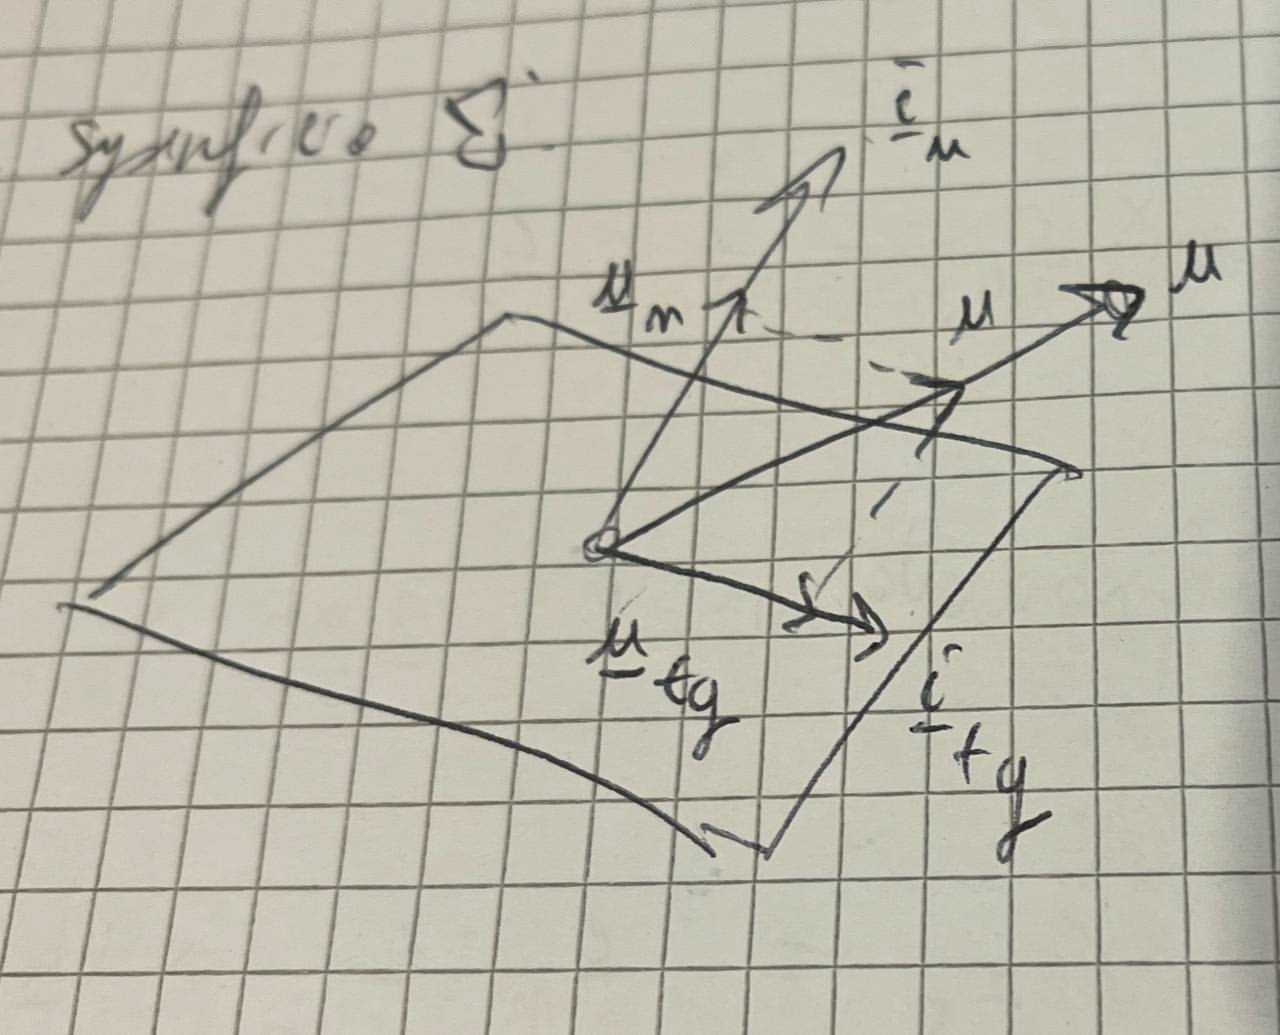
\includegraphics[width=0.60\linewidth]{img/Chapter_one/Chapt1img7.png}
        \end{figure} \\
        Si può esprimere la componente normale del generico vettore $\underline{u}$ come:
        \begin{equation}
            \underline{u}_{n} = (\underline{u} \cdot \underline{i}_{n \Sigma}) \underline{i}_{n \Sigma}
        \end{equation}
        mentre per quella tangenziale, in assenza di versore tangenziale, possiamo prendere il vettore e sottrargli la componente normale:
        \begin{equation}
            \underline{u}_{tg} = (\underline{u}-\underline{u}_{n}) = \underline{u} - (\underline{u} \cdot \underline{i}_{n \Sigma}) i_{n \Sigma}
        \end{equation}
        il quale è un doppio prodotto vettoriale\footnote{$(\underline{a} \times \underline{b}) \times c = (\underline{a} \cdot \underline{c}) \underline{b} - (\underline{b} \cdot \underline{c})\underline{a}$} che si può riscrivere come:
        \begin{equation}
        \label{eqn:componente_tangente}
            (\underline{i}_{n \Sigma} \times \underline{u}) \times \underline{i}_{n \Sigma}
        \end{equation}
        che è l'espressione della componente tangente di $\underline{u}$. Se confrontiamo la (\ref{eqn:componente_tangente}) con la $(\ref{eqn:equazione_raccordo2})$ ci si rende conto che non combaciano in termini di forma. Per ottenere infatti la componente rigorosamente tangente del campo magnetico dovremmo moltiplicare vettorialmente per $\underline{i}_{n}$, perché $\underline{i}_{t} = \underline{i}_{n} \times \underline{i}_{n\Sigma}$. \\
        Per la prima legge di Maxwell abbiamo un espressione analoga:
        \begin{equation}
            \underline{i}_{n \Sigma} \times (\underline{e}_{2}-\underline{e}_{1}) = 0
        \end{equation}
        cioè le componenti tangenti\footnote{ruotate di novanta gradi} del campo elettrico si conservano, perché nella prima legge non c'è dipendenza da termini che esprimono densità superficiali.\\ Ricapitolando:
        \begin{equation}
        \begin{cases}
            \underline{i}_{n} \times (\underline{e}_{2} - \underline{e}_{1}) = 0 \\
            i_{n \Sigma} \times (\underline{h}_{2}-\underline{h}_{1}) = \underline{j}_{S} \\
            \underline{i}_{n} \cdot (\underline{d}_{2} - \underline{d}_{1}) = \rho_{S} \\
            \underline{i}_{n} \cdot (\underline{b}_{2}-\underline{b}_{1}) = 0
        \end{cases}
        \end{equation}
    \section{L'equazione di continuità}
        Dimostriamo che l'equazione di continuità è contenuta in quelle di Maxwell, non aggiungendo de facto contenuto informativo. La sua forma integrale è:
        \begin{equation}
            -\frac{\partial}{\partial t} q(V, t) = i(\partial \underline{V}, t)
        \end{equation}
        che riscritta è
        \begin{equation}
            -\frac{\partial}{\partial t} \iiint_{V} \rho dV = \oiint_{\partial V} \underline{j} \cdot \underline{i}_{n} dV 
        \end{equation}
        Sotto l'ipotesi che si possa portare la derivata sotto il segno d'integrale ed applicando il teorema di Gauss a secondo membro, scriviamo:
        \begin{equation}
            \iiint_{V} [\frac{\partial}{\partial t} \rho + \nabla \cdot \underline{j}]dV = 0
        \end{equation}
        Poiché l'equazione di continuità vale qualunque sia $V$, applichiamo il teorema di localizzazione per ricavare l'espressione differenziale:
        \begin{equation}
        \label{eqn:eq_continuità_diff}
            \frac{\partial}{\partial t} \rho + \nabla \cdot \underline{j} = 0
        \end{equation}
        La (\ref{eqn:eq_continuità_diff}) è ricavabile applicandol'operatore divergenza ad ambo membri della terza equazione di Maxwell:
        \begin{equation}
            \nabla \cdot \nabla \times \underline{h} = \nabla \cdot (\frac{\partial}{\partial t} \underline{d} + \underline{j})
        \end{equation}
        Se $\underline{d}$ è differenziabile $\nabla \cdot \frac{\partial}{\partial t} \underline{d} = \frac{\partial}{\partial t} \nabla \cdot \underline{d}$. Inoltre, in virtù del fatto che la divergenza del rotore è nulla si ottiene:
        \begin{equation}
            \frac{\partial}{\partial t} \nabla \cdot \underline{d} + \nabla \cdot \underline{j} = \frac{\partial}{\partial t} \rho + \nabla \cdot \underline{j} = 0
        \end{equation}
        QED. 
        \section{Le relazioni costitutive}
            Le relazioni costitutive legano $\underline{e}$ ed $\underline{h}$, grandezze d'ingresso, a $\underline{d},\underline{b}$ e $\underline{j}$, grandezze di uscita. Le corrispondenze ingresso-uscita sono:
            \begin{align}
                \underline{d} (\underline{r}, t) = \hat{D}[\underline{e}(\underline{r}, t), \underline{h}(\underline{r}, t)] \\
                \underline{b} (\underline{r}, t) = \hat{B}[\underline{e}(\underline{r}, t), \underline{h}(\underline{r}, t)] \\
                \underline{j} (\underline{r}, t) = \hat{J}[\underline{e}(\underline{r}, t), \underline{h}(\underline{r}, t)] 
            \end{align}
            le quali non sono corrispondenze numeriche, perché bisogna conoscere \underline{e} ed $\underline{h}$ in ogni punto dello spazio ed in ogni istante di tempo precedente a quello corrente. Al contrario, sono \textbf{corrispondenze operatoriali} e sono tali da prelevare in ingresso funzioni e restituire in uscita funzioni. \\
            Tutte le relazioni costitutive devono soddisfare le proprietà di \textit{causalità, continuità e stabilità BIBO}. Analizziamo nel dettaglio tutte e tre. \\ \\
            La causalità si divide in \textbf{debole} e \textbf{forte}. La causalità debole richiede che l'effetto non deve precedere la causa. Non ci sono relazioni causa-effetto istantanee, allora l'effetto è necessariamente successivo alla causa. Se la causa avviene nella posizione $\underline{r}$ e l'effetto nella posizione $\underline{r}'$, ci sarà un ritardo minimo pari a:
            \begin{equation}
                \Delta t_{min} = \frac{|\underline{r}-\underline{r}'|}{c}
            \end{equation}
            In altre parole, se $t$ è l'istante in cui si manifesta la causa e $t'$ quello in cui si manifesta l'effetto, deve risultare:
            \begin{equation}
            \label{eqn:caus_forte}
                |t-t'| \geq \Delta t_{min}
            \end{equation}
            La causalità forte vale se la (\ref{eqn:caus_forte}) è verificata.\footnote{Ma non se è del tipo strettamente minore, ovvero se $|t-t'|< \Delta t_{min}$}\\
            La causalità debole\footnote{anche lei non vale se è del tipo strettamente minore} è soddisfatta se:
            \begin{equation}
                t-t' \geq 0
            \end{equation}
            Ne consegue che la causalità forte include quella causale ma non viceversa. \\ \\
            La continuità richiede che il sistema al variare in maniera sempre minore della causa, fino all'annullamento della sua variazione, debba annullare di conseguenza anche la propria variazione uscita.
            La stabilità BIBO (Bounded Input Bounded Output) richiede che ad ingresso finito ci sia uscita finita. \\ \\
            Le relazioni costitutive vanno studiate per \textit{classi di mezzi}, in modo tale da studiare un caso valido per ogni membro di una data classe. Le proprietà da verificare (o no) sono:
            \begin{itemize}
                \item Linearità
                \item Non dispersività spaziale e temporale
                \item Omogeneietà spaziale e temporale\footnote{quest'ultima altresì detta stazionarietà}
                \item Isotropia
            \end{itemize}
            \subsection{Linearità}
            Noi ipotizziamo che $\underline{d}$ dipenda solo da $\underline{e}$, $\underline{b}$ solo da $\underline{h}$ e $\underline{j}$ solo da $\underline{e}$, assunzione che vale per una grande quantità di mezzi quando non sono in movimento. \\
            Un mezzo è \textbf{lineare} se risulta per due ingressi $\underline{e}_{1}$ ed $\underline{e}_{2}$ 
            \begin{equation}
            \hat{D}[c_{1}\underline{e}_{1}+c_{2}\underline{e}_{2}] = c_{1} \hat{D}[\underline{e}_{1}]+c_{2}\hat{D}[\underline{e}_{2}]
            \end{equation}
            La relazione costitutiva per $\underline{d}$\footnote{stesso discorso per $\underline{b}$ e $\underline{j}$} ha la forma:
            \begin{equation}
            \label{eqn:eq_costitutivaTemplate}
                \underline{d}(\underline{r},t) = \iiiint_{\mathbb{R}^{4}} d\underline{r}' dt' \underline{\underline{g}}(\underline{r}. \underline{r}', t, t') \underline{e}(\underline{r}', t')
            \end{equation}
            dove $\underline{\underline{g}}$ è una matrice detta \textbf{funzione diadica di Green}. È intuibile capire il perché della (\ref{eqn:eq_continuità_diff}). Sia $(\underline{r}', t')$ la posizione di una certa causa che ha effetto in $(\underline{r}, t)$. La generica relazione causa-effetto sarà del tipo:
            \begin{equation}
                \underline{d}(\underline{r}, t) = \underline{\underline{g}} \cdot\underline{e}(\underline{r}, t)
            \end{equation}
            Ma se ci sono cause per ogni punto dello spazio ed il sistema è lineare, per tenerle in conto tutte dobbiamo sommare su tutto lo spazio e dunque si ottiene la (\ref{eqn:eq_costitutivaTemplate}). Tuttavia, la (\ref{eqn:eq_costitutivaTemplate}) integra nel tempo da $-\infty$ a $+\infty$, ma i sistemi che consideriamo devono essere causali. Ciò significa che andrebbe riscritta come:
            \begin{equation}
                \underline{d}(\underline{r},t) = \iiint_{\mathbb{R}^{3}} d\underline{r}' \int_{-\infty} ^{t} dt' \underline{\underline{g}}(\underline{r}. \underline{r}', t, t') \underline{e}(\underline{r}', t')
            \end{equation}
            La (\ref{eqn:eq_costitutivaTemplate}) può essere comunque utilizzata\footnote{E noi questa utilizzeremo} se imponiamo che la funzione di Green si annulli per $t'>t$. 
            \subsection{Non dispersività}
            Un mezzo è \textbf{temporalmente non dispersivo} se l'effetto in un istante dipende da cause unicamente in quell'istante, cioè se il mezzo è "senza memoria". La \textbf{non dispersività spaziale} è definita in modo analogo e richiede che il l'effetto dipenda soltanto dalla causa nello stesso punto e non da altri. \\
            Se ora consideriamo un sistema lineare e non dispersivo nello spazio, si può scrivere:
            \begin{equation}
                \underline{d}(\underline{r},t) = \int_{\mathbb{R}} dt' \underline{\underline{g}'}(\underline{r}, t, t') \underline{e}(\underline{r}, t)
            \end{equation}
            perché $\underline{r}$ è fissato per la non dispersività e dunque possiamo definire una funzione di Green $\underline{\underline{g}'}$ tale per cui:
            \begin{equation}
                \underline{\underline{g}}(\underline{r}, \underline{r}', t, t') = \underline{\underline{g}}' (\underline{r}, t, t')\delta(\underline{r}-\underline{r}')
            \end{equation}
            \\ Ipotizziamo ora che valga la non dispersività temporale. La relazione costitutiva sarà:
            \begin{equation}
                \underline{d} (\underline{r}, t) = \iiint_{\mathbb{R}} d \underline{r}' \underline{\underline{g}}'' (\underline{r}, \underline{r}', t) \underline{e}(\underline{r},t)
            \end{equation}
            dove $\underline{\underline{g}} (\underline{r}, \underline{r}', t, t') = \underline{\underline{g}}''(\underline{r}, \underline{r}', t, t') \delta(t-t')$. \\
            La non dispersività temporale implica la non dispersività spaziale, perché le cause in altri punti da quello corrente si propagano in tempi non nulli, ma per la non dispersività temporale la causa dipende solo dall'istante corrente e non da istanti precedenti.
            Poiché la dispersività temporale implica quella spaziale, sotto tale ipotesi la (\ref{eqn:eq_costitutivaTemplate}) si può scrivere come:
            \begin{equation}
                \underline{d} (\underline{r}, t) = \underline{\underline{g}}''' (\underline{r}, t) \underline{e}(\underline{r}, t)
            \end{equation}
            con $\underline{\underline{g}} (\underline{r}, \underline{r}', t, t') = \underline{\underline{g}}'''(\underline{r}, t) \delta(\underline{r}-\underline{r}')\delta(t-t')$. \\
            Per fare una preview di quello che sarà approfondito dopo, la funzione di Green in nel caso non dispersivo è la permettività elettrica del mezzo:
            \begin{equation}
                \underline{d}(\underline{r},t) = \underline{\underline{\varepsilon}} (\underline{r}, t)\underline{e}(\underline{r}, t)
            \end{equation}
            \subsection{Omogeneità}
            Un mezzo si dice \textbf{omogeneo nel tempo}, o anche \textbf{stazionario}, se risulta $\forall t_{0}$ e $\forall \underline{e}$:
            \begin{equation}
                \hat{D} [\ \hat{\tau}_{t_{0}}[\underline{e}(\underline{r}, t)] \ ] = \hat{\tau}_{t_{0}}[\ \hat{D}[\underline{e}(\underline{r},t)]\ ]
            \end{equation}
            dove $\hat{\tau}_{t_{0}} :\hat{\tau}_{t_{0}} [\ \underline{e}(\underline{r},t) \ ] = \underline{e}(\underline{r}, t+t_{0})$ è l'operatore di traslazione temporale di valore $t_{0}$. \\ 
            In altri termini, l'omogeneità temporale richiede che l'uscita sia invariante per traslazione temporale, che è l'equivalente dell'affermare che gli operatori $\hat{D}$ e $\hat{\tau}$ commutano\footnote{Cioè l'ordine con cui vengono applicati è irrilevante, ma ovviamente è un caso speciale e non è sempre così}. \\
            Un mezzo si dice \textbf{omogeneo nello spazio} se $\forall r_{0}, \underline{e}$:
            \begin{equation}
                \hat{D} [\ \hat{\tau}_{r_{0}}[\underline{e}(\underline{r}, t)] \ ] = \hat{\tau}_{r_{0}}[\ \hat{D}[\underline{e}(\underline{r},t)]\ ]
            \end{equation}
            cioè se $\hat{D}$ e $\hat{\tau}_{r_{0}}$\footnote{l'operatore traslazione di valore $\underline{r_{0}}$ nello spazio} commutano. \\
            Nel caso in cui c'è omogeneità spaziale la relazione costitutiva generica si scrive\footnote{Nel caso semplificativo di considerare un sistema lineare con relazione ingresso-uscita non vettoriale}:
            \begin{equation}
                y(t) = \int_{\mathbb{R}} dt' g(t, t') x(t')
            \end{equation}
            Ci si chiede allora cosa succede se supponiamo che il mezzo goda anche della stazionarietà (omogeneità temporale). \\ Sia $y_{t_{0}}$ è l'uscita ottenuta dall'ingresso traslato di $t_{0}$ e $y(t-t_{0})$ l'uscita traslata di $t_{0}$:
            \begin{equation}
                y_{t_{0}}(t) = \int_{\mathbb{R}} dt' g(t, t') x(t'-t_{0})
            \end{equation}
            \begin{equation}
                y(t-t_{0}) = \int_{\mathbb{R}} dt' g(t-t_{0},t') x(t')
            \end{equation}
            Queste due termini sono uguali per la stazionarietà:
            \begin{equation}
                \int_{\mathbb{R}} dt' g(t, t') x(t'-t_{0}) = \int_{\mathbb{R}} dt' g(t-t_{0},t') x(t')
            \end{equation}
            Effettuando un cambio di variabile $t'' = t'-t_0$ si ottiene:
            \begin{equation}
                \int_{\mathbb{R}} dt' g(t, t''+t_{0}) x(t'') = \int_{\mathbb{R}} dt' g(t-t_{0},t') x(t')
            \end{equation}
            La variabile di integrazione è "muta", cioè il nome è irrilevante e $t'$ può essere benissimo uguale a $t''$ ai fine dell'integrale. Allora si può raccogliere tutto sotto un unico integrale:
            \begin{equation}
                \int_{\mathbb{R}} dt'[x(t')[g(t, t'+t_{0})-g(t-t_{0}, t')]] = 0
            \end{equation}
            Poiché questa relazione deve valere $\forall x(t)$ per ipotesi di stazionarietà spaziale, si può scegliere $x(t) = [g(t, t'-t_{0})-g(t-t_{0}, t')]$ e dunque si ottiene:
            \begin{equation}
                \int_{\mathbb{R}} dt'[g(t, t'+t_{0})-g(t-t_{0}, t')]^{2} = 0
            \end{equation}
            Poiché la quantità da integrare è non negativa, deve necessariamente verificarsi:
            \begin{equation}
                g(t, t'+t_{0})=g(t-t_{0}, t')  \qquad \forall t
            \end{equation}
            A valle di ciò, la relazione costitutiva si riduce alla convoluzione fra la funzione di Green e la $x(t)$, perché l'unico fattore rilevante per il valore dell'uscita è la \textit{differenza} fra $t$ e $t'$ e non l'istante $t'$ in sé:
            \begin{equation}
                y(t) = \int_{\mathbb{R}} dt' g(t,t')x(t) = \int_{\mathbb{R}} dt' g(t-t')x(t)
            \end{equation}

            \subsection{Richiami sulle trasformate di Fourier}
                La trasformata di Fourier di una funzione $f(t)$ è definita come:
                \begin{equation}
                    F(\omega) = \int_{\mathbb{R}} f(t)e^{-j \omega t}dt
                \end{equation}
                con la relativa antitrasformata:
                \begin{equation}
                    f(t) = \frac{1}{2\pi} \int_{\mathbb{R}} F(\omega) e^{j \omega t} d \omega
                \end{equation}
                Elenchiamo alcune proprietà della $F(\omega)$
                \begin{itemize}
                    \item Derivazione nel tempo \ \ $\mathcal{F}[\frac{d}{dt}f(t)] = j \omega F(\omega)$
                    \item Convoluzione \ \ $\mathcal{F}[f(t)*g(t)] = F(\omega) G(\omega)$
                    \item Moltiplicazione per un fasore \ \ $\mathcal{F}[f(t)e^{j \omega_{0}t}] = F(\omega - \omega_{0})$
                    \item Traslazione nel tempo \ \ $\mathcal{F}[f(t-t_{0})] = F(\omega)e^{-j \omega t_{0}}$
                \end{itemize}
                Se $f(t) \in \mathbb{R} \ \ \forall t$, cioè se è una funzione reale, si dimostra che la $F(\omega)$ è \textbf{hermitiana}, cioè tale per cui:
                \begin{equation}
                    F(- \omega) = F^{*}(\omega)
                \end{equation}
                Questa proprietà per le funzioni reali è di rapida intuzione se si applica la mera definizione della FT:
                \begin{equation}
                    F^{*}(\omega) = \int_{\mathbb{R}} [dt f(t)e^{-j \omega t}]^{*} = \int_{\mathbb{R}} dt f(t)e^{j \omega t} = \int_{\mathbb{R}} dt f(t) e^{-j(-\omega) t} = F(-\omega)
                \end{equation}
                Inoltre scrivendo la trasformata come somma di parte reale e immaginaria, si ricava che la parte reale è pari rispetto all'origine, mentre quella immaginaria è dispari:
                \begin{align}
                    F_{R}(\omega)+jF_{J}(\omega) = F_{R}(-\omega)+jF_{J}(-\omega) \\
                    \implies \begin{cases}
                        F_{R}(\omega) = F_{R}(-\omega) \\
                        F_{J}(\omega) = - F_{J}(-\omega)
                    \end{cases}
                \end{align}
                Il modulo di un numero complesso è:
                \begin{equation}
                    |F(\omega)| = \sqrt{F_{R}(\omega)^{2}+F_{J}(\omega)^{2}}
                \end{equation}
                mentre la fase è:
                \begin{equation}
                    \angle F(\omega) = \begin{cases}
                        \arctan(\frac{F_{J}}{F_{R}}) \ \ \ \ \ \ \ \ \ \ \textrm{se }  F_{R}>0 \\
                        \pi - \arctan(\frac{F_{J}}{F_{R}}) \ \ \ \textrm{se }  F_{R}<0 \\
                        \pi/2 \qquad \qquad \ \  \  \ \ \ \   \textrm{se } F_{R} = 0, F_{J}>0 \\
                        -\pi/2 \qquad \qquad \ \ \  \   \textrm{se } F_{R} = 0, F_{J}<0 \\
                        \textrm{indefinita} \qquad \ \ \ \ \  \textrm{se } F_{R},F_{J}=0
                    \end{cases}
                \end{equation}
        Se $f(t) \in \mathbb{R}$ il modulo è funzione pari mentre la fsae è dispari. A questo punto è utile dimostrare che il contenuto informativo relativo alla $F(\omega)$ è contenuto soltanto in $[0, + \infty)$. Scriviamo l'espressione dell'antitrasformata di $F(\omega)$:
        \begin{equation}
            f(t) = \frac{1}{2 \pi} \int_{\mathbb{R}} F(\omega) e^{j \omega t}d \omega = \frac{1}{2 \pi} [\int_{- \infty}  ^{0} F(\omega) d \omega e^{j \omega t}] + \int_{0} ^{+\infty} F(\omega) d \omega e^{j \omega t}
        \end{equation}
        Effettuiamo un cambio di variabile nel secondo integrale $\omega ' = \omega$:
        \begin{equation}
            = \frac{1}{2 \pi} [ \int_{0} ^{\infty} F(\omega) e^{j \omega t} d \omega + \int_{0} ^{\infty} F(-\omega ') e^{- j \omega ' t}]d \omega '  = \frac{1}{2 \pi} [ \int_{0} ^{\infty} F(\omega) e^{j \omega t} d \omega + \int_{0} ^{\infty} [F(\omega ')]^{*} (e^{ j \omega ' t)})^{*}]d \omega '
        \end{equation}
        dove nell'ultimo passaggio abbiamo sfruttato $F(\omega) = F(-\omega)$. Poiché i due integrali hanno per argomento la stessa funzione, con il secondo ha come argomento il coniugato, poiché vale:
        \begin{equation}
            z \in \mathbb{C} \implies z + z^{*} = 2 \Re[z]
        \end{equation}
        possiamo scrivere in definitiva:
        \begin{equation}
            f(t) = \frac{1}{\pi} \Re[\int_{0} ^{\infty} F(\omega)e^{j \omega t}d \omega]
        \end{equation}
        Dunque antitrasformando la trasformata di una funzione reale ci da ancora una funzione reale e questo ci piace. \\
        Un caso di estrema importanza è la trasformata di una funzione sinusoidale pura, cioè di un'onda monocromatica\footnote{A singola frequenza}
        \begin{equation}
            f(t) = A \cos{(\omega_{0}t+\varphi)}
        \end{equation}
        Calcolandone la trasformata:
        \begin{equation}
            \mathcal{F}[A \cos{(\omega_{0}t+\varphi)}] = \mathcal{F}[\frac{A}{2}e^{j(\omega_{0}+\varphi)}+\frac{A}{2}e^{-j(\omega_{0}t+\varphi)}]
        \end{equation}
        \begin{equation}
             = \frac{A}{2}e^{j \varphi} \mathcal{F}[1 \cdot e^{j \omega_{0}t}]+\frac{A}{2}\mathcal{F}[1 \cdot e^{-j \omega_{0}t}]
        \end{equation}
        Possiamo calcolare la trasformata di $f(t) = 1$ e poi traslare in frequenza, ma $f(t)=1$ non è trasformabile\footnote{Non essendo né quadato sommabile né sommabile}, dunque la trasformata va intesa nel senso delle distribuzioni. Per fare ciò, riprendiamo un utilissimo risultato. Se $F(\omega)$ è la trasformata di $f(t)$, facendo l'antitrasformata di $F(\omega)$ si ottiene:
        \begin{equation}
        \label{eqn:anti_antitrasformata}
            \mathcal{F}[F(\omega)] = \int_{\mathbb{R}} d\omega F(\omega) e^{-j \omega t} = \frac{2\pi}{2\pi} \int_{\mathbb{R}}f(\omega)e^{j \omega(-t)}d \omega = 2 \pi f(-t)
        \end{equation}
        A valle del fatto che la trasformata della $\delta$ è:
        \begin{equation}
            \mathcal{F}[\delta] = 1
        \end{equation}
        Utilizzando la (\ref{eqn:anti_antitrasformata}) otteniamo:
        \begin{equation}
            \mathcal{F}[1] = 2 \pi \delta(-t) = 2\pi \delta(t)
        \end{equation}
        In definitiva, la trasformata di un'onda monocromatica è:
        \begin{equation}
            \mathcal{F}[A \cos{(\omega_{0}t)}+\varphi] = A \pi e^{j \varphi}\delta(\omega-\omega_{0})+A \pi e^{-j \varphi}\delta(\omega+\omega_{0})
        \end{equation}
        Se $A$ è l'ampiezza del seno e ha dimensioni, per esempio, di un campo elettrico ($\displaystyle\frac{V}{m}$), la trasformata avrà dimensioni $\displaystyle \frac{V \cdot s}{m}$\footnote{La FT è un integrale in $dt$}, perché la delta in questo caso ha le dimensioni di un tempo. Tuttavia, per un tono puro la pulsazione $\omega_{0}$ è fissata e dunque il contenuto informativo è contenuto tutto in:
        \begin{equation}
            \bar{F} = Ae^{j \varphi} \implies F(\omega) = \pi \bar{F}\delta(\omega-\omega_{0})+\pi \bar{F}^{*}\delta(\omega+\omega_{0})
        \end{equation}
        dove $\bar{F}$ è chiamato \textbf{fasore} ed ha le stesse dimensioni della funzione originale $f(t)$, nel nostro esempio quelle di un campo elettrico. Il fasore, nel caso di una funzione sinusodiale pura, definisce in modo \textbf{univoco}. Infatti, tornando indietro con l'antitrasformata, poiché le grandezze fisiche sono sicuramente descritte da funzioni reali si ottiene:
        \begin{equation}
            f(t) = \frac{1}{\\pi} \Re[\int_{0} ^{\infty} \pi\overline{F}\delta(\omega-\omega_{0})e^{j \omega t}d \omega] = \Re[\overline{F}e^{j \omega_{0}t}]
        \end{equation}
        dove abbiamo escluso il termine associato al fasore $\overline{F}^{*}$ perché centrato in $-\omega_{0} < 0$.
        \\ \\
        La trasformata di Fourier è uno strumento potente per manipolare le equazioni di Maxwell. Nel caso di una rete reale con elementi dissipativi\footnote{Per esempio i resistori} ci si aspetta che l'evoluzione libera decada all'infinito lasciando semplicemente la forzata, dunque c'è il problema dovuto al fatto di non poter considerare, operando nel dominio trasformato, le condizioni iniziali. Questa cosa però è problematica nel caso in cui le linee siano idealizzate affinché siano senza perdite (lossless).
        
        \subsection{Isotropia}
            Se l'omogeneità esprimeva, per un mezzo materiale, l'invarianza per traslazione, l'isotropia esprime l'invarianza di questo per rotazione. Distinguiamo due tipi di isotropia, di \textit{forma} e di \textit{materiale}. La prima è legata alla forma del mezzo mentre la seconda alla composizione atomica del materiale. \\
            Per definire l'isotropia materiale, consideriamo una forma invariante per traslazione attorno a qualunque asse passante per il suo centro: la sfera. Inoltre, dobbiamo assumere che il mezzo sia non dispersivo nello spazio. \\
            Una rotazione attorno ad un asse è individuata da un vettore $\underline{\varphi}$. Il suo modulo esprime l'entità della rotazione mentre i suoi coseni direttori\footnote{cioè le componenti del vettore normalizzate al modulo dello stesso} il verso e la direzione della rotazione. Per determinare il verso orario od antiorario della rotazione si utilizza la regola della mano destra.
            \begin{figure}[h!]
                \centering
                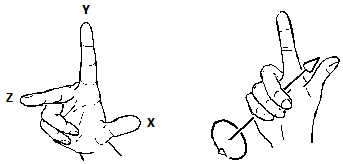
\includegraphics[width=0.5\linewidth]{img//Chapter_one/chaptOneManoDestra.png}
            \end{figure}
            \\
            Introduciamo l'operatore di rotazione $\hat{R}_{\underline{\varphi}}$ che effettua una rotazione attorno all'asse di rotazione specificata da $\underline{\varphi}$. Un mezzo è isotropo se risulta:
            \begin{equation}
                \hat{D}[\hat{R}_{\underline{\varphi}}(\underline{e}(\underline{r}, t))] = \hat{R}_{\underline{\varphi}}[\hat{D}(\underline{e}(\underline{r}, t))]  
            \end{equation}
            \\
            Assumendo ora che il mezzo sia anche non dispersivo nel tempo, dimostriamo che l'isotropia implica che la causa e l'effetto siano allineati, cioè che i vettori rappresentanti causa ed effetto siano fra loro proporzionali. \\
            Ipotizziamo che $\underline{e}(\underline{r},t)$ (causa) e $\underline{d}(\underline{r},t)$ (effetto) non siano tra loro allineati come in figura:
            \begin{figure}[h!]
                \centering
                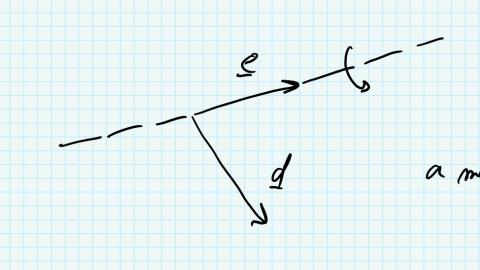
\includegraphics[width=0.5\linewidth]{img//Chapter_one/chaptOneIsotropia.png}
                \label{fig:isotropia}
                \caption{}
            \end{figure} \\
            Applicando una rotazione attorno all'asse corrispondente alla direzione di $\underline{e}(\underline{r},t)$, questo rimane invariato perché la rotazione di un vettore parallelo a quello di rotazione $\underline{\varphi}$ ritorna lo stesso vettore. Ciò però non si può dire per la causa, che invece varia. Ma poiché in principio abbiamo assunto che il mezzo sia isotropo, l'unica possibilità per la quale $\underline{d}(\underline{r},t)$ rimanga invariato per rotazione è che sia allineato a $\underline{e}(\underline{r},t)$. \\
            In generale non vale il contrario, cioè l'allineamento di $\underline{e}(\underline{r},t)$ e $\underline{d}(\underline{r},t)$ non implica l'isotropia. Per visualizzarlo, consideriamo un mezzo con la seguente relazione costitutiva:
            \begin{equation}
                \label{eqn:rel_cost_esempio}
                \underline{d}(\underline{r},t) = a(t) (\underline{e}(\underline{r},t) \cdot \underline{i}_{x})\underline{e}(\underline{r},t)
            \end{equation}
            Dalla (\ref{eqn:rel_cost_esempio}) traiamo le proprietà del mezzo: esso è non lineare (dipende dal prodotto per qualcosa che dipende da $\underline{e}(\underline{r},t)$), non dispersivo in $t$ ed in $\underline{r}$ (perché non c'è l'integrale in $\mathbb{R} ^{4}$), omogeneo nello spazio ed anisotropo\footnote{Per verificare l'anisotropia, valutare l'effetto della rotazione con due ingressi diversi, prima lungo l'asse $x$ e poi lungo $y$. Il secondo si annulla nel prodotto interno con $\underline{i}_{x}$, ottenendo in definitiva un risultato diverso da quello generato dal primo ingresso}.
            \\ \\
            Supponiamo ora di avere un mezzo lineare non dispersivo nel tempo e, come assunto già prima, nello spazio. Il risultato che stiamo per ottenere vale anche in assenza di non dispersività temporale. Vogliamo dimostrare la seguente catena di implicazioni:
            \begin{equation}
                \textrm{Isotropia} \implies \textrm{causa ed effetto allineati} \implies \underline{\underline{\varepsilon}} = \varepsilon \underline{\underline{I}} \implies \textrm{Isotropia}
            \end{equation}
            Cioè stiamo ambendo a dimostrare che per un mezzo lineare e non dispersivo nello spazio e nel tempo, se la causa e l'effetto sono allineati allora il mezzo è isotropo. La prima implicazione è stata dimostrata sopra. Per dimostrare la seconda, scriviamo la relazione costitutiva per un mezzo lineare e non dispersivo nello spazio e nel tempo:
            \begin{equation}
            \label{eqn:matricione1}
                \begin{pmatrix}
                    d_{x} \\
                    d_{y} \\
                    d_{z}
                \end{pmatrix} = 
                \begin{pmatrix}
                    \varepsilon_{xx} & \varepsilon_{xy} & \varepsilon_{xz} \\ 
                    \varepsilon_{yx} & \varepsilon_{yy} & \varepsilon_{yz} \\
                    \varepsilon_{zx} & \varepsilon_{zy} & \varepsilon_{zz} \\
                \end{pmatrix} \cdot 
                \begin{pmatrix}
                    e_{x} \\
                    e_{y} \\
                    e_{z}
                \end{pmatrix}
            \end{equation}
            dove l'elemento $\varepsilon_{ij}$ della matrice di permettività elettrica è la risposta in uscita lungo la direzione $i$ all'ingresso lungo la direzione $j$. Supponiamo di avere un ingresso lungo $x$:
            \begin{equation}
                \underline{e} = e_{0}\underline{i}_{x} = (e_{0} \quad 0 \quad 0\ )
            \end{equation}
            Sostituendo nella (\ref{eqn:matricione1}) otteniamo, sviluppando il prodotto matriciale a secondo membro:
            \begin{equation}
                \begin{cases}
                    d_{x} = \varepsilon_{xx} e_{0} \\
                    d_{y} = \varepsilon_{yx} e_{0} \\
                    d_{z} = \varepsilon_{zx} e_{0}
                \end{cases}
            \end{equation}
            Poiché causa ed effetto sono allineati, le risposte in uscita lungo $x$ dovute ad ingressi $y$ e $z$ devono essere nulle:
            \begin{equation}
                \varepsilon_{yx}=\varepsilon_{zx} = 0
            \end{equation}
            Iterando lo stesso procedimento per ingresso solo lungo $z$ e lungo $y$ si ottiene\footnote{Non è stato specificato in classe, ma ciò che ci permette di sommare i risultati ottenuti è la linearità, perché il generico ingresso di componenti $x,y,z$ può essere visto come combinazione lineare di ingressi lungo le singole direzioni}:
            \begin{equation}
            \label{eqn:matricione2}
                \underline{\underline{\varepsilon}} = \begin{pmatrix}
                    \varepsilon_{xx} & 0 & 0 \\
                    0 & \varepsilon_{yx} & 0 \\
                    0 & 0 & \varepsilon_{zx}
                \end{pmatrix}
            \end{equation}
            Affinché la permettività magnetica si possa scrivere come prodotto per la matrice identità $\underline{\underline{I}}$ ed una costante $\varepsilon$, dobbiamo dimostrare che i tre termini sulla diagonale siano tutti uguali. Consideriamo un ulteriore ingresso con componenti sul piano $xy$:
            \begin{equation}
                \underline{e} = e_{x}\underline{i}_{x}+e_{y}\underline{i}_{y}
            \end{equation}
            Sostituendo nella (\ref{eqn:matricione1}) e tenendo conto della (\ref{eqn:matricione2}) si ottiene:
            \begin{equation}
                \begin{cases}
                    d_{x} = \varepsilon_{xx}e_{x} \\
                    d_{y} = \varepsilon_{yy}e_{y}
                \end{cases}
            \end{equation}
            Dividendo membro a membro:
            \begin{equation}
            \label{eqn:matricione3}
                \frac{d_{y}}{d_{x}} = \frac{\varepsilon_{yy}}{\varepsilon_{xx}} \frac{\varepsilon_{y}}{\varepsilon_{x}}
            \end{equation}
            Disegnando i due vettori nel piano $xy$ ci si rende conto che (\ref{eqn:matricione3}) si può scrivere come:
            \begin{equation}
                \tan(\psi_{d}) = \frac{\varepsilon_{xx}}{\varepsilon_{yy}} \tan(\psi_{e})
            \end{equation}
            Ma se i due vettori sono allineati, allora hanno lo stesso angolo rispetto all'asse $x$ e di conseguenza:
            \begin{equation}
                \psi_{d} = \psi_{e} \implies \varepsilon_{xx} = \varepsilon_{yy}
            \end{equation}
            Reiterando il ragionamento per un ingresso nel piano $yz$ si arriva a:
            \begin{equation}
                \varepsilon_{xx} = \varepsilon_{yy} =\varepsilon_{zz} = \varepsilon
            \end{equation}
            \begin{figure}[h!]
                \centering
                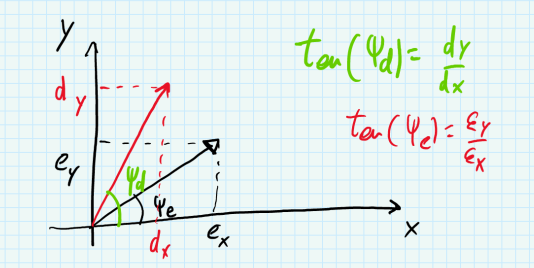
\includegraphics[width=0.5\linewidth]{img//Chapter_one/chaptOneMatricione.png}
            \end{figure}
            Resta da dimostrare l'ultima implicazione. A valle di ciò che abbiamo appena mostrato:
            \begin{equation}
                \underline{d}(\underline{r},t) = \varepsilon \underline{e}(\underline{r},t)
            \end{equation}
            Se applichiamo l'operatore di rotazione, che è un operatore lineare, la $\varepsilon$ che è una costante esce fuori dall'espressione e dunque si ottiene:
            \begin{equation}
                \hat{R}_{\underline{\varphi}}[\underline{d}(\underline{r},t)] = \varepsilon \hat{R}_{\underline{\varphi}}[\underline{e}(\underline{r},t)]
            \end{equation}
            ma causa ed effetto sono allineati e dunque la direzione di $\underline{d}$ ed $\underline{e}$ è la stessa, ragion per cui il mezzo è isotropo.

    \subsection{I mezzi normali e le relazioni nel dominio della frequenza}
        Un mezzo è detto \textbf{normale} se ha le seguenti proprietà:
        \begin{itemize}
            \item È lineare
            \item È non dispersivo nello spazio
            \item È stazionario
            \item È isotropo
        \end{itemize}
        A valle della definizione, le relazioni costitutive sono:
        \begin{equation}
            \begin{cases}
                \displaystyle\underline{d}(\underline{r},t) = \int_{\mathbb{R}}dt' g_{d}(\underline{r}, t-t')\underline{e}(\underline{r},t) \\
                \displaystyle\underline{b}(\underline{r},t) = \int_{\mathbb{R}}dt' g_{b}(\underline{r}, t-t')\underline{h}(\underline{r},t) \\
                \underline{j}(\underline{r}, t) = \sigma (\underline{r}) \cdot \underline{e}(\underline{r},t)
            \end{cases}
        \end{equation}
        Delle tre equazioni appena scritte, quella per la densità di corrente fa eccezione circa l'assunzione che il mezzo sia non dispersivo nel tempo, il quale ci permette di far saltare l'integrale e definire la conducibilità elettrica $\sigma(\underline{r})$. La proprietà di dispersività tuttavia rimane per $\underline{d}$ e $\underline{b}$. \\ \\
        Nel dominio di Fourier le stesse relazioni si scrivono come:
        \begin{equation}
            \begin{cases}
            
            \underline{D}(\underline{r},\omega) = \varepsilon (\underline{r}, \omega) \underline{E}(\underline{r}, \omega) \\
            \underline{B}(\underline{r} ,\omega) = \mu ( \underline{r}, \omega)  \underline{H}(\underline{r}, \omega) \\
            \underline{J}(\underline{r} ,\omega) = \sigma(\underline{r}) \underline{E}(\underline{r}, \omega)
            \end{cases}
        \end{equation}
        Analizziamo queste espressioni. Prima di tutto, sono prodotti di trasformate, perché nel tempo quegli integrali sono di convoluzione. In secundis, la permettività elettrica $\underline{\varepsilon}(\underline{r},t)$ e quella magnetica $\underline{\mu}(\underline{r},t)$ (che sono rispettivamente le trasformate di $g_{d}(\underline{r},t)$ e $g_{b}(\underline{r},t)$) dipendono dalla frequenza, cioè sono \textbf{dispersive in frequenza}. Un materiale è dispersivo in frequenza se il suo comportamento varia al variare della frequenza. Nel tempo, questo corrisponde alla dispersività nel tempo. Infatti, se il materiale è senza memoria (non dispersivo in $t$) l'integrale nel tempo salta e si ottiene:
        \begin{equation}
            \begin{cases}
            
            \underline{D}(\underline{r},\omega) = \varepsilon (\underline{r}) \underline{E}(\underline{r}, \omega) \\
            
            \underline{B}(\underline{r} ,\omega) = \mu ( \underline{r})\underline{H}(\underline{r}, \omega) \\
            
            \end{cases}
        \end{equation}
        ovvero la non dipendenza della funzione di Green ($\varepsilon$ e $\mu$ nel nostro caso) dalla frequenza. \\ \\
        Le equazioni di Maxwell, similmente, assumono questa forma qui:
        \begin{equation}
            \begin{cases}
            \nabla \times \underline{E} = - j \omega \underline{B} \\
            \nabla \times \underline{H} = j \omega \underline{D} + \underline{J} + \underline{J}_{0} \\
            \nabla \cdot \underline{D} = \rho + \rho_{0} \\
            \nabla \cdot \underline{B} = 0
            \end{cases}
        \end{equation}
    \section{Teoremi di unicità}
        Riprendiamo il discorso delle condizioni al contorno. Bisogna ricorrere ai teoremi di unicità, che offrono condizioni sufficienti (ma non necessarie!) a determinare univocamente la soluzione. I problemi di unicità sono classificati in quattro categorie:
        \begin{itemize}
            \item Problema interiore con soluzione nel tempo 
            \item Problema interiore con soluzione in frequenza
            
            \item Problema esteriore con soluzione nel tempo 
            \item Problema esteriore con soluzione in frequenza
        \end{itemize}
        Il problema è interiore quando si cerca la soluzione in un dominio $V$ limitato nello spazio, mentre è esteriore quando tale soluzione è cercata nel \textit{complemento} di un dominio limitato. Noi analizziamo i quattro casi considerando mezzi normali.
        \subsection{Problema tempo interiore}
        Iniziamo ad analizzare il caso "tempo-interiore" per cercare la soluzione nel dominio $V$. Assumendo la non dispersività temporale, assieme alle equazioni di Maxwell, che evito di riscrivere, bisogna scrivere le condizioni all'istante iniziale $t_{0}$:
        \begin{equation}
            \begin{cases}
                \underline{e}(\underline{r},t_{0}) = \underline{e}_{0}(\underline{r}) \\
                \underline{b}(\underline{r},t_{0}) = \underline{b}_{0}(\underline{r})
            \end{cases} \quad \forall \underline{r} \in V
        \end{equation}
        Vanno poi aggiunte le equazioni costitutive per un mezzo normale non dispersivo in $t$:
        \begin{equation}
        \begin{cases}
            \underline{d}(\underline{r},t) = \varepsilon(\underline{r}) \underline{e}(\underline{r},t) \\
            \underline{b}(\underline{r},t) = \mu (\underline{r}) \underline{h}(\underline{r},t) \\
            \underline{j}(\underline{r},t) = \sigma ( \underline{r}) \underline{e}(\underline{r},t)
        \end{cases}
        \end{equation}
        Ultime ma non meno importanti le condizioni al raccordo:
        \begin{equation}
            \underline{i}_{n} \times \underline{e}(\underline{r}, t) = \underline{e}_{tg}(\underline{r},t) \qquad \underline{r} \in \partial V, \ \ t \geq t_{0}
        \end{equation}
        Il teorema di unicità per il problema tempo interiore afferma che date queste informazioni, cioè equazioni di Maxwell, raccordo, costitutive e condizioni iniziali, la soluzione se esiste è unica. Il teorema di unicità è una condizione sufficiente ma non necessaria. \\
        Per dimostrare il teorema, introduciamo il \textbf{vettore di Poynting}, la cui trattazione è posticipata ai capitoli successivi:
        \begin{equation}
            \underline{s} = \underline{e} \times \underline{h}
        \end{equation}
        Calcoliamo allora la divergenza del vettore di Poynting:
        \begin{equation}
            \nabla \cdot \underline{s}  = \nabla \cdot (\underline{e} \times \underline{h}) = \nabla \times \underline{e} \cdot \underline{h}-\underline{e} \nabla \times \underline{h}
        \end{equation}
        dove nell'ultimo passaggio abbiamo utilizzato un'identità vettoriale notevole.\footnote{$\nabla \cdot (\underline{a} \times \underline{b}) = \nabla \times \underline{a} \cdot \underline{b} - \underline{a} \cdot \nabla \times \underline{b}$}
        Sostituendo le espressioni dei rotori di $\underline{e}$ ed $\underline{h}$ dateci dalle equazioni di Maxwell:
        \begin{equation}
            \nabla \cdot \underline{s} = (-\frac{\partial}{\partial t} \underline{b})\cdot \underline{h}-\underline{e} \cdot (\frac{\partial}{\partial t}\underline{d}+\underline{j}+\underline{j}_{0})
        \end{equation}
        Riordinando l'equazione si ottiene \textbf{l'identità di Poynting in forma locale}:
        \begin{equation}
            \nabla \cdot \underline{s} +\underline{h} \cdot \frac{\partial}{\partial t} \underline{b}+\underline{e} \cdot \frac{\partial}{\partial t}\underline{d}+\underline{e} \cdot \underline{j}= \underline{e} \cdot \underline{j}_{0}
        \end{equation}
        Si ottiene l'identità di Poynting in forma integrale semplicemente integrando su $V$ e applicando il teorema di Gauss per la divergenza di $\underline{s}$ si ottiene:
        \begin{equation}
            \oiint_{\partial V} \underline{s} \cdot \underline{i}_{n} dS + \iiint_{V} ( \underline{h} \cdot \frac{\partial}{\partial t} \underline{b}+\underline{e}\cdot \frac{\partial}{\partial t} \underline{d})dV + \iiint_{V} \underline{e} \cdot \underline{j}dV = - \iiint_{V} \underline{e} \cdot \underline{j}_{0} dV
        \end{equation}
        Finora non abbiamo sfruttato le ipotesi nel mezzo, ma non è mai tardi per cambiare idea.
        Sostituiamo le relazioni costitutive per un mezzo normale non dispersivo nel tempo:
        \begin{equation}
            \underline{b} = \mu \cdot \underline{h} \quad \underline{d} = \varepsilon \cdot \underline{e} \quad \underline{j} = \sigma \cdot \underline{e}
        \end{equation}
        \begin{equation}
            \implies \nabla \cdot \underline{s} + \underline{h} \frac{\partial}{\partial t}(\mu \cdot \underline{b})+\underline{e} \cdot \frac{\partial}{\partial t}(\varepsilon \cdot \underline{e})+(\sigma \cdot \underline{e}) \cdot \underline{e} = -\underline{e} \cdot \underline{j}_{0}
        \end{equation}
        Invocando la stazionarietà, $\mu$, $\varepsilon$ e $\sigma$ escono fuori dalle derivate. Notiamo che possiamo scrivere:
        \begin{equation}
           \mu \cdot \underline{h} \cdot \frac{\partial}{\partial t} (\underline{h}) = \frac{\mu}{2} \cdot \frac{\partial}{\partial t} (\underline{h}^{2}) = \frac{\mu}{2} \cdot \frac{\partial}{\partial t}|h|^{2}
        \end{equation}
        \begin{equation}
            \varepsilon \cdot \underline{e} \cdot \frac{\partial}{\partial t} \underline{e} = \varepsilon \frac{\partial}{\partial t} |\underline{e}|^{2}
        \end{equation}
        \begin{equation}
            \sigma \underline{e} \cdot \underline{e} = \sigma |e|^{2}
        \end{equation}
        potendo scrivere, in definitiva:
        \begin{equation}
            \nabla \cdot \underline{s} + \frac{\partial}{\partial t}(\frac{\mu}{2} |\underline{h}|^{2}+\frac{\varepsilon}{2}|\underline{e}|^{2}) + \sigma |\underline{e}|^{2} = - \underline{e} \cdot \underline{j}_{0}
        \end{equation}
        ovvero l'identità di Poynting in forma locale per mezzi normali non dispersivi.
        Per la forma integrale, ammesso che $V$ non vari nel tempo:
        \begin{equation}
            \oiint_{\partial V} \underline{s} \cdot \underline{i}_{n} dS + \frac{d}{dt}\iiint_{V} \frac{\mu}{2} |\underline{h}|^{2}+\frac{\varepsilon}{2}|\underline{e}|^{2}dV + \iiint_{V} \sigma |\underline{e}|^{2} dV = - \iiint_{V} \underline{e}\cdot \underline{j}_{0}dV
        \end{equation}
        Importante notare il simbolo di derivata totale rispetto al tempo al posto di quella parziale, in quanto la dipendenza spaziale di $\underline{e}$ ed $\underline{h}$ viene persa a causa dell'integrazione in $V$. \\ \\
        Ora possiamo finalmente dimostrare il teorema di unicità per il caso tempo-interno. 
        Supponiamo che la soluzione esista e che per assurdo sia non unica, dunque ce ne sono almeno due, per esempio $(\underline{e}_{1}, \underline{h}_{1})$ e $(\underline{e}_{2}, \underline{h}_{2})$. \\
        Sostituiamo le equazioni costitutive all'interno di quelle di Maxwell, ottenendo un sistema con sole incognite $\underline{e}$ ed $\underline{h}$.
        \begin{equation}
            \begin{cases}
            \nabla \times \underline{e} = - \displaystyle \mu \cdot \frac{\partial}{\partial t} \underline{h} \\
            \nabla \times \underline{h} = \displaystyle \varepsilon \cdot \frac{\partial}{\partial t} \underline{e} +  \sigma \underline{e} +\underline{j}_{0}\\
            \nabla \cdot \underline{\varepsilon \underline{e}} = \rho + \rho_{0} \\
            \nabla \cdot (\mu \underline{h}) =0
            \end{cases}
        \end{equation}
        Si tenga conto che $\underline{j}$ è ricavabile conoscendo $\underline{e}$ ed $\underline{h}$ in virtù dell'equazione di continuità\footnote{Che ricordiamo essere $\nabla \cdot j = - \displaystyle \frac{\partial}{\partial t}\rho $}.\\
        Definiamo i vettori differenza $\underline{e}_{d}$ ed $\underline{h}_{d}$:
        \begin{equation}
            \begin{cases}
                \underline{e}_{d} = \underline{e}_{1}-\underline{e}_{2} \\
                \underline{h}_{d} = \underline{h}_{1} - \underline{h}_{2}
            \end{cases}
        \end{equation}
        Vogliamo verificare che siano anch'essi campi elettromagnetici. Se $\underline{e}_{1}$ ed $\underline{e}_{2}$, così come $\underline{h}_{1}$ ed $\underline{h}_{2}$, sono soluzioni, allora devono soddisfare le equazioni di Maxwell. Se sostituiamo nella prima, si ottiene:
        \begin{equation}
        \begin{cases}
            \nabla \times \underline{e}_{1} = -  \displaystyle \mu \frac{\partial}{\partial t} \underline{h}_{1} \\
            \nabla \times \underline{e}_{2} = - \mu \frac{\partial}{\partial t} \underline{h}_{2}
        \end{cases} \implies \nabla \times (\underline{e}_{2}-\underline{e}_{1}) = - \mu \frac{\partial}{\partial t}(\underline{h}_{2}-\underline{h}_{1})
        \end{equation}
        ovvero:
        \begin{equation}
            \nabla \times \underline{e}_{d} = - \mu \frac{\partial}{\partial t} \underline{h}_{d}
        \end{equation}
        La prima è soddisfatta. Reiterando il ragionamento, anche la seconda è soddisfatta \textbf{ma con termine noto nullo}:
        \begin{equation}
        \begin{cases}
            \nabla \times \underline{h}_{1} = \displaystyle \varepsilon \cdot \frac{\partial}{\partial t} \underline{e}_{1} + \sigma \underline{e}_{1} + \underline{j}_{0} \\
            
            \nabla \times \underline{h}_{2} = \displaystyle \varepsilon \cdot \frac{\partial}{\partial t} \underline{e}_{2} + \sigma \underline{e}_{2} + \underline{j}_{0}
        \end{cases} \implies \nabla  \times \underline{h}_{d} = \varepsilon \frac{\partial}{\partial t} \underline{e}_{d} + \sigma \underline{e}_{d}
        \end{equation}
        Similmente, per la terza si ricava:
        \begin{equation}
            \varepsilon \nabla \cdot \underline{e}_{d} = \rho_{d}
        \end{equation}
        mentre della quarta è inutile discutere. \\
        Otteniamo in definitiva un sistema di equazioni omogenee:
        \begin{equation}
        \begin{cases}
            \nabla \times \underline{e}_{d} = - \displaystyle \mu \frac{\partial}{\partial t} \underline{h}_{d} \\
            \nabla \times \underline{h}_{d} = \displaystyle \varepsilon \frac{\partial}{\partial t} \underline{e}_{d}+\sigma \cdot \underline{e}_{d} \\
            \nabla \cdot (\varepsilon \underline{e}_{d}) = \rho \\
            \nabla \cdot (\mu \underline{h}_{d} )= 0
        \end{cases}
        \end{equation}
        Poiché le due soluzioni che abbiamo supposto valide prima hanno le stesse condizioni iniziali ed al contorno, quelle relative ai vettori differenza sono nulle:
        \begin{equation}
            \begin{cases}
                \underline{e}_{d} (\underline{r},t_{0}) = 0 \\
                \underline{h}_{d} (\underline{r},t_{0})=0
            \end{cases}
        \end{equation}
        \begin{equation}
            \underline{i}_{n} \times \underline{e}_{d}(\underline{r},t) = 0
        \end{equation}
        Segue che i vettori differenza sono campi elettromagnetici. Applicando Poynting per mezzi normali non dispersivi nel tempo:
        \begin{equation}
            \oiint_{\partial V} \underline{s}_{d} \cdot \underline{i}_{n} dS + \frac{d}{dt} \iiint_{V} (\frac{\mu}{2} |\underline{h}_{d}|^{2}+\frac{\varepsilon}{2}|\underline{e}|^{2})dV + \iiint_{V} \sigma |\underline{e}_{d}|^{2}dV = - \iiint_{V} \underline{e} \cdot \underline{j}_{0}dV
        \end{equation}
        Il termine:
        \begin{equation}
            \iiint_{V} \underline{e} \cdot \underline{j}_{0}dV
        \end{equation}
        va a zero perché per i vettori differenza i termini noti sono nulli. Similmente, esprimendo $\underline{s}_{d}$:
        \begin{equation}
            \underline{s}_{d} = \underline{e}_{d} \times \underline{h}_{d} \cdot \underline{i}_{n} = \underline{i}_{n} \times \underline{e}_{d} \cdot \underline{h}_{d} = 0 \cdot \underline{h}_{d} = 0
        \end{equation}
        avendo sfruttato le condizioni al contorno per i vettori differenza.
        Supponendo che:
        \begin{equation}
            \begin{cases}
                \mu > 0 \\
                \varepsilon > 0 \\
                \sigma \geq 0
            \end{cases}
        \end{equation}
        e definendo:
        \begin{equation}
            P_{j}(t) = \iiint_{V} \sigma |\underline{e}|^{2}dV \qquad W(t) = \iiint_{V} (\frac{\mu}{2}|\underline{h}|^{2}+\frac{\varepsilon}{2}|\underline{e}|^{2})dV
        \end{equation}
        si ricava dall'identità di Poynting:
        \begin{equation}
            \frac{d}{dt}W(t) = - P_{J}(t)
        \end{equation}
        In virtù delle ipotesi su $\sigma, \varepsilon$ e $\mu$, si ottiene $P_{J}(t) \geq 0 \ \ \forall t$ e dunque la derivata di $W(t)$ è non positiva. Ciò significa che:
        \begin{equation}
            t \geq t' \implies W(t) \geq W(t')
        \end{equation}
        Per cui fissato l'istante iniziale $t_{0}$:
        \begin{equation}
            W(t_{0}) \geq W(t) \quad \forall t \geq t_{0}
        \end{equation}
        Tuttavia, per come $W(t)$ è definita, sotto le ipotesi fatte per $\sigma, \varepsilon$ e $\mu$, è una funzione semidefinita positiva, cioè $W(t) \geq 0$. Dunque:
        \begin{equation}
            0 \leq W(t) \leq 0 \implies W(t) = \iiint_{V} \frac{\mu}{2}|\underline{h}_{d}|^{2}+\frac{\varepsilon}{2}|\underline{e}_{d}|^{2}dV = 0
        \end{equation}
        Si può passare dall'integrale all'integrando nullo perché l'integrando è semidefinito nel segno, in quanto ci sono tutte quantità non negative. L'unico modo per il quale l'integrando si annulla, poiché $\mu >0$ e $\varepsilon>0$ è:
        \begin{equation}
            |\underline{h}_{d}|^{2} = |\underline{e}_{d}|^{2} = 0 \implies \underline{h_{1}}=\underline{h}_{2} \qquad \underline{e}_{1} = \underline{e}_{2}
        \end{equation}
        QED. \\ \\
        Se avessimo assegnato come condizione al contorno:
        \begin{equation}
            \underline{i}_{n} \times \underline{h} = \underline{h}_{tg}
        \end{equation}
        bastava fare una permutazione circolare diversa per l'espressione di $\underline{s}_{d}$ e trovare lo stesso risultato. \textbf{Non} si possono dare entambe le condizioni perché se do una identifico univocamente anche l'altra. In altre parole, se ho sia la condizione di contorno per il campo elettrico che per quello magnetico il sistema di equazioni è incompatibile e non ammette soluzione.
        \newpage
        \subsection{Problema tempo-esteriore}
            Per il problema tempo esteriore, dobbiamo considerare il complemento di un dominio limitato, per esempio:
            \begin{figure}[h!]
                \centering
                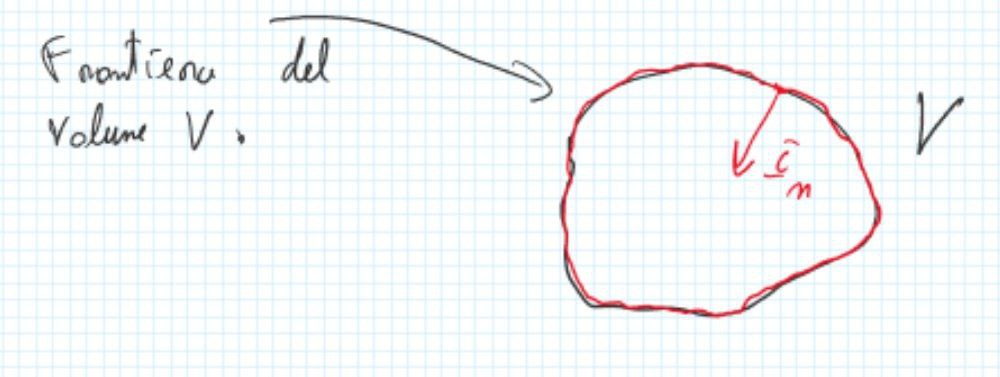
\includegraphics[width=0.5\linewidth]{img//Chapter_one/Chapt1img8.png}
            \end{figure}
        Se consideriamo una superficie sferica sufficientemente grande che racchiude una buona porzione di spazio attorno a $V$, potremmo pensare di risolvere il problema esteriore come un problema interiore nella regione di spazio intermedio fra $V$ e la frontiera della superficie sferica. Il problema è che non si conoscono le condizioni del campo sulla frontiera di tale sfera. \\
        Ipotizziamo allora di stare nelle condizioni per cui il campo è zero definitivamente in un intorno dell'infinito, cioè esiste sempre un intorno dell'infinito per il quale il campo è nullo. Questo ha senso se si considera la causalità forte, che richieda lo scorrere di un intervallo di tempo non nullo affinché gli effetti delle sorgenti si propaghino nello spazio. Tutto questo ragionamento crolla per la soluzione a regime, dove di tempo ne è passato idealmente infinito rispetto all'accensione delle sorgenti di campo, abbastanza per raggiungere ogni punto dello spazio con gli effetti. \\ 
        In definitiva, la risoluzione del problema tempo-esteriore deriva direttamente da quella del caso tempo-interiore, nel caso in cui non sia interessati alla soluzione a regime.

    \subsection{Problema omega-interiore}
        Il teorema di unicità omega-interiore richiede che vengano fornite le equazioni di Maxwell:
        \begin{equation}
        \begin{cases}
            \nabla \times \underline{E} = -j \omega \underline{B} \\
            \nabla \times \underline{D} = j \omega \underline{D}+\underline{J}+\underline{J}_{0} \\
            \nabla \cdot \underline{D} = \rho \\
            \nabla \cdot \underline{B} = 0
        \end{cases}
        \end{equation}
        le relazioni costitutive - nel nostro caso per i mezzi normali:
        \begin{equation}
            \begin{cases}
                \underline{D}(\underline{r},\omega) = \varepsilon(\underline{r})  \underline{E}(\underline{r},\omega) \\
                \underline{B}(\underline{r},\omega) = \mu(\underline{r})\underline{H}(\underline{r},\omega) \\
                \underline{J}(\underline{r},\omega) = \sigma(\underline{r})\underline{E}(\underline{r},\omega)
            \end{cases}
        \end{equation}
        e infine le relazioni al contorno:
        \begin{equation}
            \underline{i}_{n} \times \underline{E}|_{\partial V} = \underline{E}_{tg}
        \end{equation}
        dove $\underline{i}_{n} \times E|_{\partial V}$ è la componente tangente\footnote{ruotata di $\pi/2$ ndr} del campo elettrico calcolata sulla frontiera di $V$. \\
        Delle condizioni iniziali non ce ne facciamo niente perché 1) stiamo cercando la soluzione in regime sinusoidale e 2)in frequenza per includerle si dovrebbe fare un casino matematico.
        Il teorema afferma che date queste informazioni la soluzione se esiste è unica in \textbf{a meno di condizioni risonanti}. \\ \\
        Procediamo in modo analogo a quanto fatto per il tempo interiore introducendo il vettore di Poynting nel dominio della frequenza:
        \begin{equation}
            \underline{S}=\frac{1}{2}\underline{E} \times \underline{H}^{*}
        \end{equation}
        Calcoliamone a divergenza:
        \begin{equation}
            \nabla \cdot \underline{S} = \nabla \cdot (\frac{1}{2}\underline{E} \times \underline{H}^{*}) = \frac{1}{2}[\nabla \times \underline{E} \cdot \underline{H}^{*}- \underline{E} \cdot \nabla \times \underline{H}^{*}]
        \end{equation}
        Sostituiamo le equazioni di Maxwell per levare $\underline{D}$ e $\underline{B}$:
        \begin{equation}
            \nabla \cdot \underline{S} = j \frac{\omega}{2}(\mu \underline{H}) \cdot \underline{H}^{*}-j \frac{\omega}{2}(\varepsilon \underline{E})^{*}\cdot \underline{E} + \frac{1}{2}\underline{E} \cdot (\sigma \underline{E})^{*}  \frac{1}{2}\underline{E} \cdot \underline{J}_{0} 
        \end{equation}
        A valle che fatto che $\sigma$ non dipende dal tempo, la sua trasformata in $\omega$ è un numero reale, mentre $\mu$ e $\varepsilon$ sono complessi:
        \begin{equation}
            \nabla \cdot \underline{S} = j \frac{\omega}{2}\mu\cdot  (\underline{H} \cdot \underline{H}^{*})-j \frac{\omega}{2}\varepsilon^{*} (\underline{E}^{*}\cdot \underline{E}) + \frac{1}{2}\sigma^{*}(\underline{E} \cdot  \underline{E}^{*}) = -\frac{1}{2} \underline{E}\cdot \underline{J}_{0}
        \end{equation}
        Riconosciamo nell'espressione i moduli di $\underline{H} $ ed $ \underline{E}$\footnote{Vedi appendice A per note sulla norma dei vettori complessi}, potendo dunque scrivere:
        \begin{equation}
        \label{eqn:rel_stronza}
            \nabla \cdot \underline{S} +j \omega \frac{\mu}{2}|\underline{H}|^{2}-j \frac{\omega}{2}\varepsilon^{*}|\underline{E}|^{2}+\frac{\sigma}{2}|\underline{E}|^{2}=-\frac{1}{2}\underline{E} \cdot \underline{J}_{0}
        \end{equation} \\
        Scomponiamo la (\ref{eqn:rel_stronza}) come coppia di equazioni, una alla parte reale e una alla parte immaginaria di $\nabla \cdot \underline{S}$. Posto:
        \begin{equation}
            \underline{S}=\underline{S}_{R}+j\underline{S}_{I} \qquad \varepsilon=\varepsilon'-j\varepsilon'' \qquad \mu = \mu'-j\mu''
        \end{equation}
        dove $\varepsilon''$ e $\mu''$ sono gli opposti delle parti immaginarie di $\varepsilon$ e $\mu$, definite per facilità di calcolo, si può scrivere per quella reale:
        \begin{equation}
            \nabla \cdot \underline{S}_{R} = \Re[j \frac{\omega}{2}\mu |H|^{2}]-\Re[j \frac{\omega}{2}\varepsilon^{*}|E^{2}|]+\Re[\frac{\sigma}{2}|E|^{2}]-\frac{1}{2}\Re[\underline{E}\cdot \underline{J}_{0}]
        \end{equation}
        \begin{equation}
            \implies 
            \nabla \cdot \underline{S}_{R} = \frac{\omega}{2}|H|^{2}\Re[j \mu]-|E^{2}|\frac{\omega}{2}\Re[j \varepsilon^{*}]+\frac{\sigma}{2}|E|^{2}-\frac{1}{2}\Re[\underline{E}\cdot \underline{J}_{0}]
        \end{equation}
        Ora poiché $z \in \mathbb{C} \implies \Re[j z]=-\Im[z]$\footnote{$\Re[jz] = \Re[jz_{R}-z_{I}] = -z_{I}$}, si ottiene:
        \begin{equation}
            \Re[j\mu] = \mu '' \qquad \Re[j \varepsilon^{*}] = - \varepsilon''
        \end{equation}
        Ottenendo:
        \begin{equation}
            \nabla \cdot \underline{S}_{R}+\frac{\omega}{2}|\underline{H}|^{2}\mu''+\frac{\omega}{2}|\underline{E}|^{2}\varepsilon''+\frac{\sigma}{2}|\underline{E}|^{2}=-\Re[\frac{1}{2}\underline{E}\cdot \underline{J}_{0}]
        \end{equation}
        Mentre per la parte immaginaria\footnote{dove abbiamo rimosso a priori $\sigma |\underline{E}|^{2}$ che è totalmente reale}:
        \begin{equation}
            \nabla \underline{S}_{I} +\frac{\omega}{2}|\underline{H}|^{2} \textrm{Im}[j \mu]-\frac{\omega}{2}|\underline{E}|^{2}\textrm{Im}[j \varepsilon^{*}] = - \textrm{Im}[\frac{1}{2}\underline{E}\cdot \underline{J}_{0}]
        \end{equation}
        Ottenendo, in virtù di $\textrm{Im}[jz]=\Re[z]$:
        \begin{equation}
            \nabla \cdot \underline{S}_{I}+\frac{\omega}{2}|\underline{H}|^{2}\mu'-\frac{\omega}{2}|\underline{E}|^{2}\varepsilon'=-\textrm{Im}[\frac{1}{2}\underline{E}\cdot \underline{J}_{0}]
        \end{equation}
        Mettendo a sistema, ricaviamo l'identità di Poynting in forma locale come equazioni alla parte reale e immaginaria:
        \begin{equation}
        \begin{cases}
            \nabla \cdot \underline{S}_{R}+\frac{\omega}{2}|\underline{H}|^{2}\mu''+\frac{\omega}{2}|\underline{E}|^{2}\varepsilon''+\frac{\sigma}{2}|\underline{E}|^{2}=-\Re[\frac{1}{2}\underline{E}\cdot \underline{J}_{0}] \\
             \nabla \cdot \underline{S}_{I}+\frac{\omega}{2}|\underline{H}|^{2}\mu'-\frac{\omega}{2}|\underline{E}|^{2}\varepsilon'=-\textrm{Im}[\frac{1}{2}\underline{E}\cdot \underline{J}_{0}]
        \end{cases}
        \end{equation}
        Per passare alla forma integrale, si raccoglie un $2\omega$ alla parte immaginaria per convenzione e si integra in $V$, applicando Gauss per il flusso di $\underline{S}$:
        \begin{equation}
            \begin{cases}
             \displaystyle \oiint_{\partial V}  \underline{S}_{R} \cdot \underline{i}_{n}dV+\iiint_{V} (\frac{\omega}{2}|\underline{H}|^{2}\mu''+\frac{\omega}{2}|\underline{E}|^{2}\varepsilon'')dV+\iiint_{V}\frac{\sigma}{2}|\underline{E}|^{2}dV=-\Re[\iiint_{V}\frac{1}{2}\underline{E}\cdot \underline{J}_{0} dV] \\ \\
             \displaystyle \oiint_{\partial V}  \underline{S}_{I} \cdot \underline{i}_{n}+ 2 \omega\iiint_{V} \frac{\omega}{4}|\underline{H}|^{2}\mu'dV-2 \omega\iiint_{V}\frac{\omega}{4}|\underline{E}|^{2}\varepsilon'dV=-\textrm{Im}[\iiint_{V}\frac{1}{2}\underline{E}\cdot \underline{J}_{0}dV]
        \end{cases}
        \end{equation}
         \\ \\
         Ricavata l'identità di Poynting in frequenza, possiamo dimostrare il teorema. In modo analogo al caso tempo-interiore, ipotizziamo per assurdo che ci siano almeno due soluzioni $(\underline{E}_{1}, \underline{H}_{1})$ e $(\underline{E}_{2}, \underline{H}_{2})$. Diamo per assodato che i vettori differenza:
         \begin{equation}
             \underline{E}_{d} = \underline{E}_{1}-\underline{E}_{2} \qquad \underline{H}_{d}=\underline{H}_{1}-\underline{H}_{2}
         \end{equation}
         soddisfino le equazioni di Maxwell con condizioni al raccordo e termini noti nulli, come abbiamo fatto vedere nel caso temporale sostituendo le soluzioni nelle relazioni e sottraendo membro a membro:
         \begin{equation}
             \rho_{0, d} = 0 \qquad J_{0, d} = \underline{0} \qquad  \underline{i}_{n} \times \underline{E}_{d}|_{\partial V}  = \underline{0}
         \end{equation}
         Applichiamo l'identità di Poynting tenendo conto di quanto appena scritto per i vettori differenza. Come nel caso tempo-interno, il flusso del vettore di Poynting risulta nullo in virtù della nullità della componente tangente del campo elettrico $E_{tg, d}$
         \begin{equation}
             \underline{S}_{d} \cdot \underline{i}_{n}=\frac{1}{2} \underline{E}_{d} \times \underline{H}_{d} \cdot \underline{i}_{n} =\frac{1}{2} \underline{i}_{n} \times \underline{E}_{d} \cdot \underline{H}_{d} = \frac{1}{2} \cdot 0 \cdot \underline{H}_{d} = 0
         \end{equation}
         In modo analogo, i termini a secondo membro dell'identità di Poynting, sia per la parte reale che immaginaria, sono nulli per la nullità di $\underline{J}_{0, d}$. Scriviamo in definitiva:
         \begin{equation}
             \begin{cases}
                 \displaystyle \iiint_{V}\frac{\mu''}{2}|\underline{H}|^{2}+\frac{\varepsilon''}{2}|\underline{E}|dV+\iiint_{V} \frac{\sigma}{2}|\underline{E}_{d}|^{2}dV = 0 \\ \\

                \displaystyle 2 \omega [\iiint_{V} \frac{\mu''}{4}|\underline{H}|^{2}dV - \iiint_{V} \frac{\varepsilon'}{4}|\underline{E}|^{2}dV]= 0
             \end{cases}
         \end{equation}
Ipotizziamo:
\begin{equation}
    \begin{cases}
        \omega \varepsilon''>0 \\
        \omega \mu'' > 0 \\
        \sigma \geq 0
    \end{cases} \qquad \qquad \omega \neq 0
\end{equation}
Le trasformate delle funzioni di Green $\mu, \varepsilon$ e $\sigma$ sono trasformate di funzioni reali, dunque il loro spettro è hermitiano. Per simmetria hermitiana, la parte immaginaria è una funzione dispari. Poiché la funzione $y=\omega$ è dispari\footnote{È la bisettrice del primo quadrante} allora le $\omega \varepsilon''$ ed $\omega \mu''$ sono funzioni pari, dunque sono positive per omega positive, zero per omega nulle e negative altrimenti. Consideriamo allora l'equazione per la parte reale:
\begin{equation}
    \iiint_{V}\frac{\mu''}{2}|\underline{H}|^{2}+\frac{\varepsilon''}{2}|\underline{E}|dV+\iiint_{V} \frac{\sigma}{2}|\underline{E}_{d}|^{2}dV = 0
\end{equation}
L'integrale  è nullo perché semidefinito nel segno. Si può passare all'integrando nullo perché le quantità sotto segno di integrale sono tutte non negative, per cui vale la legge di annullamento del prodotto. L'unico modo per cui l'espressione è nulla è che:
\begin{equation}
    |\underline{H}_{d}|=|\underline{E}_{d}|=0
\end{equation}
da cui la tesi.
Ipotizziamo ora che $\omega \mu'' = 0, \sigma =0, \omega \varepsilon''>0$. In tal caso sostituendo nella relazione per la parte reale risulta $|\underline{E_{d}}|=0$. Sostituendo poi nella prima equazione di Maxwell:
\begin{equation}
    \nabla \times \underline{E}_{d} = 0 = -j \omega \mu \underline{H}_{d} \implies \underline{H}_{d}=0
\end{equation}
da cui di nuovo l'unicità della soluzione. Possiamo reiterare lo stesso ragionamento ponendo una variable maggiore di zero e le altre due nulle. Cosa accade se sono tutte e tre nulle? Che l'equazione parte reale si annulla, non potendone ricavare alcuna informazione, mentre quella parte immaginaria diventa:
\begin{equation}
    \iiint_{V} \frac{\mu'}{4}|\underline{H}_{d}|^{2}dV = \iiint_{V} \frac{\varepsilon'}{4}|\underline{E}_{d}|^{2}dV
\end{equation}
In tal caso la soluzione non è unica e l'unico costringente che si ha è l'uguaglianza integrale che abbiamo appena scritto: questo è il caso delle \textbf{soluzioni risonanti}. Fisicamente parlando, la parte reale è costituta dai termini del problema elettromagnetico responsabili delle perdite di energia. Nel caso di soluzione risonante, il circuito oscilla in modo indefinito in assenza sia di forzamenti interni, dovuti a $\rho_{0}$ e $\underline{J}_{0}$, che esterni, dovuti alle condizioni al contorno che rappresentano l'influenza dei campi elettromagnetici esterni.

\subsection{Problema omega-esteriore}
    Nel caso temporale, abbiamo considerato soluzioni non a regime, per avvalerci del fatto che esiste sempre un intorno di infinito per il quale il campo è definitivamente nullo. Per le soluzioni in frequenza, che nel nostro caso sono sempre a regime sinusoidale, non possiamo più fare questa cosa senza ipotizzare che valga la seguente:
    \begin{equation}
        \lim_{\underline{r} \to \infty} \underline{r}(\underline{E}-\zeta \underline{H} \times \underline{i}_{r}) = 0
    \end{equation}
    detta \textbf{condizione di radiazione all'infinito} oppure di \textbf{Silver-M{\"u}ller}. La tesi, che non dimostriamo, afferma che sotto tale ipotesi la soluzione se esiste è unica e non possono esserci soluzioni risonanti. Intuitivamente\footnote{l'espressione che segue è da considerarsi una chiacchiera da bar, non pretende di essere formale} questa cosa è associata al fatto che la radiazione propagandosi all'infinito senza tornare indietro si porti appresso dell'energia, la quale viene sottratta al sistema fino ad esaurirsi.
\section{Il teorema di Poynting}
    \subsection{Energia legata al campo elettromagnetico}
        Il primo principio della termodinamica afferma che la variazione dell'energia interna $U$
        di un sistema fisico varia in accordo agli scambi energetici del sistema con l'esterno.
        In altre parole, la variazione di energia interna è pari alla variazione di calore $\delta Q$ e lavoro $\delta L$:
        \begin{equation}
            \label{eqn:primo_principio_termodinamica}
            d U = \delta Q+\delta L
        \end{equation}
    \subsection{Teorema di Poynting nel dominio del tempo}
        Fatta l'ipotesi di mezzo normale non dispersivo nel tempo, vale la già discussa identità di Poynting in forma integrale:
        \begin{equation}
            \label{eqn:Poynting_integrale_tempo}
            \oiint_{\partial V} \underline{s} \cdot \underline{i}_{n}dS+\frac{d}{dt}\iiint_{V}(\frac{\mu}{2}|\underline{h}|^{2}+\frac{\varepsilon}{2}|\underline{e}|^{2})dV +
            \iiint_{V}\sigma |\underline{e}|^{2}dV = - \iiint_{V} \underline{e}\cdot \underline{j}_{0}dV
        \end{equation}
        L'obiettivo di questa sottosezione è ricostruire l'identità di Poynting in modo analogo alla (\ref{eqn:primo_principio_termodinamica}), per associare ad ogni pezzo della
        (\ref{eqn:Poynting_integrale_tempo}) il suo significato fisico. \\
        Partiamo dall'espressione della forza di Lorentz esercitata su di una carica $q$:
        \begin{equation}
            \underline{F}= q \underline{e}+q \underline{r} \times \underline{b}
        \end{equation}
        La forza di Lorentz è un approccio macroscopico al problema della forza esercitata su di una carica immersa in un campo elettromagnetico, perché compare la densità di carica
        elettrica $\rho$, dunque le cariche vengono immaginate come un continuo nello spazio. Consideriamo allora un volumetto $\Delta V$ con all'interno carica $\Delta q$.
        Calcolando la forza di Lorentz esercitata su tale volumetto di carica:
        \begin{equation}
            \Delta \underline{F} = \Delta q\underline{e}+\Delta q \underline{r}\times \underline{b}
        \end{equation}
        Passiamo alla densità di forza, (misurata in $N/m^{3}$) dividendo per $\Delta V$ e facendo il limite per $\Delta V \to 0$:
        \begin{equation}
            \label{eqn:densitaForza}
            \lim_{\Delta V \to \infty} \frac{\Delta \underline{F}}{\Delta V} = \underline{f}(\underline{r},t) = \rho(\underline{r},t)\underline{e}(\underline{r},t)+\rho(\underline{r},t)\underline{v}\times \underline{b}(\underline{r},t)
        \end{equation}
        Il primo addendo della (\ref{eqn:densitaForza}) deriva direttamente della definizione di densità di carica, semplicemente il limite del rapporto $\Delta q/\Delta V$.
        Per capire che significato abbia il secondo addendo, consideriamo una superficie con piana orientata lungo l'asse $x$, cioè con $\underline{i}_{n} = \underline{i}_{x}$:
        \begin{figure}[h!]
            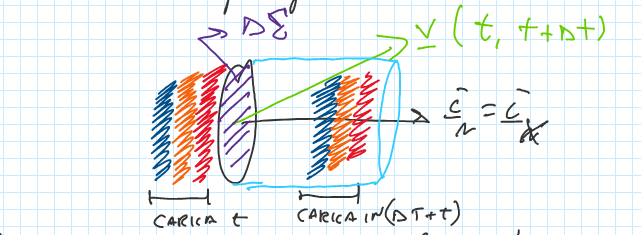
\includegraphics[width=0.6\linewidth]{img/Chapter_one/Chapt1img9.png}
        \end{figure}
        Tale superficie è attraversata con vettore velocità $\underline{v}$ da una certa carica $\Delta q$ nell'intervallo $[t, t+\Delta t]$.
        Dunque la carica totale che attraversa la porzione dello spazio evidenziata in blu è data da
        \footnote{Rigorosamente bisognerebbe integrare nel tempo e nello spazio, ma per semplificare lo scriviamo come prodotto delle quantità infinitesime $\Delta \Sigma_{x}$ e $\Delta t$}:
        \begin{equation}
            \Delta q = \rho \Delta \Sigma_{x}v_{x}\Delta t
        \end{equation}
        dove $v_{x} = \underline{v} \cdot \underline{i}_{x}$ è la proiezione di $\underline{v}$ sull'asse $\underline{x}$. Per ottenere la componente lungo $x$ della densità di corrente dividiamo per $\Delta \Sigma_{x}\Delta t$:
        \begin{equation}
                j_{x}=\frac{\Delta q}{\Delta \Sigma_{x}\delta t} = \frac{\rho \Delta v_{x}\Delta \Sigma_{x}\Delta t}{\Delta \Sigma_{x}\Delta t}=\rho v_{x}
        \end{equation}
        Dunque la densità di corrente è legata alla velocità delle cariche tramite la densità di carica, relazione che non stupisce se si tiene conto che $\rho$ da informazioni circa la posizione delle cariche nello spazio.
        Il discorso è analogo per $j_{y}$ e $j_{z}$. Sostituendo nella (\ref{eqn:densitaForza}) si ottiene:
        \begin{equation}
            \underline{f}(\underline{r},t)=\rho(\underline{r},t)\underline{e}(\underline{r},t)+\underline{j}(\underline{r},t)\times \underline{b}(\underline{r},t)
        \end{equation}
        Moltiplicando per la velocità, si ottiene la potenza per unità di volume\footnote{Infatti se il lavoro è $W=\underline{F} \cdot \underline{s}$, la potenza sarà $P= \frac{d}{dt}(\underline{F}\cdot \underline{s})=\underline{F}\cdot \underline{v}$}:
        \begin{equation}
            \label{eqn:densità_potenza_erogata}
            \underline{f} \cdot \underline{v} = \rho \underline{e} \cdot \underline{v}+\underline{j}\times \underline{b}\cdot \underline{v} = 
            \rho \underline{e} \cdot \underline{v}+\rho \underline{v}\times \underline{b}\cdot \underline{v} = \rho \underline{e} \cdot \underline{v} = \underline{e} \cdot \underline{j}
        \end{equation}
        Abbiamo annullato il secondo termine perché compare un prodotto misto con due vettori paralleli, in questo caso $\underline{j}$ e $\underline{v}$.
        Dalla (\ref{eqn:densità_potenza_erogata}) ricaviamo il significato di:
        \begin{equation}
            \label{eqn:da_campo_a_impresse}
            \iiint_{V} \underline{e} \cdot \underline{j}_{0}
        \end{equation}
        che è la potenza\footnote{ottenuta tramite una densità di potenza integrata nello spazio} erogata dal campo elettromagnetico alle sorgenti impresse, rappresentate da $\underline{j}_{0}$.
        Poiché però nell'identità di Poynting la (\ref{eqn:da_campo_a_impresse}) compare con un meno davanti, il tutto rappresenta la potenza fornita dalle sorgenti impresse al campo elettromagnetico.
        \\ In maniera analoga, la quantità:
        \begin{equation}
            \iiint_{V} \underline{e} \cdot \underline{j} = \iiint_{V} \sigma |\underline{e}|^{2}dVV
        \end{equation}
        è la quantità di potenza che il campo fornisce alle sorgenti indotte, cioè quanta potenza questo spende per tenere in vita tali sorgenti. Notiamo che
        per come è definita, questa quantità è non negativa, perché:
        \begin{equation}
            \label{eqn:equazione_che_mi_serve}
            \begin{cases}
                \underline{j} = \sigma \underline{e} \\
                \underline{j}=\rho \underline{v}
            \end{cases} \implies \rho \underline{v} = \sigma \underline{e}
        \end{equation}
        da cui si ricava $\sigma \geq 0$, perché se le cariche sono positive devono avere lo stesso verso del campo elettrico e viceversa. \\
        La quantità $\sigma |\underline{e}|^{2}$ è responsabile della forza, ma dalla (\ref{eqn:equazione_che_mi_serve}) risulta che se tale termine è costante si ha velocità costante,
        contrariamente all'aspettativa che questa debba aumentare. Questa relazione però ha pieno senso fisico, perché il campo deve erogare una potenza costante per sostenere
        le sorgenti indotte, che dissipano potenza in calore tramite gli urti con le vibrazioni reticolari. Nel nostro caso, l'energia fornite alle indotte è non negativa, cioè il 
        trasferimento di potenza è unidirezionale dal campo verso le indotte, ragion per la quale si può parlare di \textbf{potenza dissipata per effetto Joule}:
        \begin{equation}
            P_{J} = \iiint_{V} \sigma |\underline{e}|^{2}dV
        \end{equation}
        \\ \\
        Concentriamoci ora sul primo pezzo del membro di sinistra dell'identità di Poynting, ignorando per ora il significato del vettore di Poynting. Riportiamo l'identità:
        \begin{equation}
            \frac{d}{dt} \iiint_{V} \frac{\mu}{2}|\underline{h}|^{2}+\frac{\varepsilon}{2}|\underline{e}|^{2}dV+ \iiint_{V} \sigma |\underline{e}|^{2}dV = - \iiint_{V}\underline{e}\cdot \underline{j}dV
        \end{equation}
        Moltiplichiamo ambo membri per $dt$:
        \begin{equation}
            d \iiint_{V} \frac{\mu}{2}|\underline{h}|^{2}+\frac{\varepsilon}{2}|\underline{e}|^{2}dV+ dt\iiint_{V} \sigma |\underline{e}|^{2}dV = -dt \iiint_{V}\underline{e}\cdot \underline{j}dV
        \end{equation}
        Le potenze trasferite alle indotte e alle impresse, moltiplicate per $dt$, assumono le dimensioni di un energia, dunque il termine:
        \begin{equation}
            dW(t) = d \iiint_{V} \frac{\mu}{2}|\underline{h}|^{2}+\frac{\varepsilon}{2}|\underline{e}|^{2}dV = \iiint_{V} w_{m}+w_{e} dV
        \end{equation}
        non è altro che la variazione di energia del campo elettromagnetico $dW(t)$, con $w_{e} = \frac{\varepsilon}{2}|\underline{e}|^{2}$ 
        e $w_{m}=\frac{\mu}{2}|\underline{h}|^{2}$ rispettivamente la densità di energia elettrica e magnetica. Da questa relazione ricaviamo $\varepsilon>0$ e 
        $\mu >0$, perché se per assurdo fossero negative avremmo energia gratis, in quanto per una variazione negativa dell'energia interna l'ambiente avrebbe fornito calore. Allo stesso modo
        non possono essere nulle, perché per variazione nulla di energia intera il sistema avrebbe fornito calore. Posto $w_{em}= w_{e}+w_{m}$, ci si rende conto 
        che l'energia elettromagnetica $W(t)$ è proprio il termine $U$ riportato nel primo principio della termodinamica, -$\delta Q$ è il calore dissipato per effetto Joule\footnote{dove c'è un meno per via del fatto che si trova a primo membro e non a secondo}
        e $\delta L$ il lavoro fornito al sistema tramite le sorgenti impresse :
        \begin{equation}
                dU(t) = dW(t) = dt\iiint_{V} w(t)dV \qquad -\delta Q =P_{J}   \qquad \delta L = - \iiint_{V} \underline{e} \cdot \underline{j}_{0}dV
        \end{equation}
        \begin{equation}
            \implies dU-\delta Q = \delta L \implies dU = \delta Q + \delta L
        \end{equation}
    Affrontiamo ora il discorso sul significato del vettore di Poynting e sul perché abbiamo potuto ignorarlo finora.
    Quando il campo elettromagnetico attraversa la frontiera $\partial V$ del dominio $V$, lo fa trasportando energia. Ciò
    che tiene conto di tale quantità è il flusso del vettore di Poynting, che corrisponde alla potenza istantanea uscente
    trasportata dal campo elettromagnetico attraverso la frontiera del volume. Dunque $\underline{s}$ ha le dimensioni
    di una densità superficiale di potenza, misurata in $W/m^{2}$. \\
    Il motivo per il quale abbiamo potuto trascurarlo è che, considerato un volume abbastanza grande per cui
    la sua superficie cade in un intorno dell'infinito, per sorgenti di campo attivate ad istanti finiti\footnote{cioè non accese da $-\infty$, altrimenti
    il ragionamento crolla} il campo si può considerare nullo alla superficie e dunque anche il trasferimento di potenza istantanea su di essa.
    \subsection{Teorema di Poynting nel dominio dei fasori}
        Nel dominio dei fasori il teorema di Poynting è più generale, perché non è richiesta l'ipotesi di non dispersività
        temporale.\footnote{Se il mezzo è non dispersivo, la relazione costitutiva è una convoluzione temporale, la quale diventa il prodotto
        in frequenza che abbiamo visto nel paragrafo 1.5.3} All'interno di questa sezione, come prima, il nostro interesse
        è ricavare il significato fisico dei pezzi che compongono l'identità di Poynting in frequenza. 
        \\ \\ Partiamo con il giustificare la definizione:
        \begin{equation}
            \underline{S} = \frac{1}{2}\underline{E} \times \underline{H}^{*}
        \end{equation} \\
        Consideriamo un bipolo all'interno di un circuito a regime sinusoidale con corrente\footnote{qui ho messo il cappello ai fasori, ci vorrebbe anche
        quando scrivo i fasori dei campi, che avendo già il sottolineato per i vettori ometto per bellezza} $\overline{I}$
        e tensione $\overline{V}$. Nel tempo, la potenza assorbita/dissipata dal bipolo è data da:
        \begin{equation}
            p(t) = v(t)i(t)=V_{m}\cos{(\omega t + \varphi_{v})}I_{m}\cos{(\omega t + \varphi_{i})}
        \end{equation}
        Utilizzando le formule di Werner, $\cos{(a)}\cos{(b)} = \frac{1}{2}[\cos{(a+b)}+\cos{a-b}]$:
        \begin{equation}
            p(t) = \frac{1}{2}V_{m}I_{m}[\cos{(2\omega t + \varphi_{v}+\varphi_{i})}+\cos{( \varphi_{v}-\varphi_{i})}]
        \end{equation}
        Calcoliamo allora la potenza media:
        \begin{equation}
            <p(t)> = \frac{1}{T} \int_{0} ^{T} \frac{1}{2}V_{m}I_{m}[\cos{(2\omega t + \varphi_{v}+\varphi_{i})}+\cos{( \varphi_{v}-\varphi_{i})}] dt
        \end{equation}
        Il primo coseno si annulla sul periodo $T$ perché è periodico di $T/2$, mentre il secondo è costante rispetto ad $\omega$. In definitiva:
        \begin{equation}
            <p(t)>=\frac{1}{2}V_{m}I_{m}\cos{(\varphi_{v}-\varphi_{i})} = \frac{1}{2}V_{m}I_{m}\Re[e^{j(\varphi_{v}-\varphi_{i})}] = \Re[\frac{1}{2}V_{m}e^{j\varphi_{v}}I_{m}e^{-j\varphi_{i}}]
        \end{equation}
        Il termine $\overline{V}=V_{m}e^{j \varphi_{v}}$ è il fasore associato a $v(t)$, mentre $\overline{I}^{*}=I_{m}e^{-j\varphi_{i}}$ è il
        coniugato del fasore associato ad $i(t)$. Dunque possiamo scrivere la potenza \textbf{media} come la parte reale di:
        \begin{equation}
                <p(t)>=\Re[\frac{1}{2}\overline{V} \ \overline{I^{*}}]
        \end{equation}
        Definiamo allora la potenza complessa:
        \begin{equation}
            \label{eqn:potenza_media}
            \hat{P} = \frac{1}{2}\overline{V} \ \overline{I^{*}} = P+jQ
        \end{equation}
        dove $P$ è la potenza attiva, corrispondente alla potenza media, mentre $Q$ è la potenza reattiva,
        la quale non ha significato fisico. La potenza reattiva è un indicatore della qualità dello scambio energetico.
        Se infatti scriviamo la \ref{eqn:potenza_media} come parte reale di un numero complesso:
        \begin{equation}
            P=\frac{1}{2}|\overline{V}||\overline{I}|\cos{(\Delta \varphi)}
        \end{equation}
        con $\Delta \varphi = \varphi_{v}-\varphi_{i}$, ci si rende conto che $|I|\cos{(\Delta \varphi)}$ non è altro
        che la proiezione di $I$ sul piano reale. Al variare del modulo di $I$, la potenza media rimane la stessa, perché varia
        allo stesso tempo $\varphi_{i}$ e dunque lo sfasamento "controbilancia" il modulo. Tuttavia, se la potenza media è sempre la stessa,
        a noi interessa che il modulo della corrente sia il più piccolo possibile, perché se c'è più corrente sulla
        linea viene dissipata più potenza. Dunque una potenza reattiva $Q=0$ corrisponde a trasferimento di potenza massimo sulla linea. \\ \\
        Tutto ciò che abbiamo detto per tensione e corrente si può generalizzare per confronto con il prodotto di due quantità sinusodiali
        qualsiasi, nel nostro caso $\underline{e}$ ed $\underline{h}$ e i relativi fasori $\underline{E}$ ed $\underline{H}$.
        Riprendiamo di nuovo l'identità di Poynting  inetgrale nel tempo per un mezzo normale ma non necessariamente dispersivo:
        \begin{equation}
            \oiint_{\partial V} \underline{i}_{n}dS = \iiint_{V} (\underline{h}\cdot \frac{\partial}{\partial t}\underline{b}+\underline{e}\cdot \frac{\partial}{\partial t}\underline{d})dV+
            \iiint_{V} \sigma |\underline{e}|^{2}dV = - \iiint_{V} \underline{e} \cdot \underline{j}_{0}dV
        \end{equation}
        Confrontiamo pezzo per pezzo con la sua controparte fasoriale. Le quantità:
        \begin{equation}
            \sigma |e^{2}| = \underline{e} \cdot \underline{j} \qquad \underline{e}\cdot \underline{j}_{0}
        \end{equation}
        sappiamo essere rispettivamente le densità di potenza dissipata per le indotte e fornita dalle impresse.
        In modo analogo a (\ref{eqn:potenza_media}) possiamo scrivere:
        \begin{equation}
             \underline{e} \cdot \underline{j} = \Re [\frac{1}{2}\underline{E}\cdot \underline{J}^{*}] 
             \qquad \underline{e}\cdot \underline{j}_{0} = \Re [\frac{1}{2}\underline{E}\cdot \underline{J}^{*}_{0}]
        \end{equation} 
        cioè come le parti reali di di densità di potenze medie. In modo simile, il pezzo:
        \begin{equation}
            \omega\frac{\mu ''}{2}|\underline{H}|^{2}+\omega \frac{\varepsilon ''}{2}|E|^{2}
        \end{equation}
        Se calcoliamo il valore medio di $\underline{h} \cdot \frac{\partial}{\partial t} \underline{b}$ otteniamo di nuovo espressioni
        come parti reali di densità di potenza:
        \begin{equation}
            <\underline{h} \cdot \frac{\partial}{\partial t} \underline{b}> = \frac{1}{2}\Re[\underline{H} \cdot (j \omega \underline{B})^{*}] =
            \frac{\omega}{2}\Re[-j \underline{H} \cdot (\mu \underline{H})^{*}] 
        \end{equation}
        \begin{equation}
            = \frac{\omega}{2}\Re[-\mu^{*}j \underline{H} \cdot \underline{H}^{*}] = - \frac{\omega}{2}|\underline{H}|^{2}\Re[j \mu^{*}]
            =\frac{\omega}{2}\mu '' |\underline{H}|^{2}
        \end{equation}
        Allo stesso modo:
        \begin{equation}
            <\underline{e} \cdot \frac{\partial}{ \partial t} \underline{d}> = \frac{\omega}{2}\varepsilon '' |\underline{H}|^{2}
        \end{equation}
        Il termine:
        \begin{equation}
            \iiint_{V} (\underline{h} \cdot \frac{\partial}{\partial t} \underline{b} + \underline{e} \cdot \frac{\partial}{\partial t} \underline{d}) dV
        \end{equation}
        tiene conto sia della variazione dell'energia immagazzinata $\frac{d}{dt}W(t)$ che della potenza dissipata per altri motivi
        oltre all'effetto Joule $p_{d}(t)$. Ma in regime sinusoidale:
        \begin{equation}
            <\frac{d}{dt}W(t)> = \frac{1}{T} \int_{0} ^{T} \frac{d}{dt}W(t)dt = \frac{1}{T}[W(T)-W(0)] = 0
        \end{equation}
        perché l'energia è anch'essa una funzione sinusoidale di periodo $T/2$. Allora quel termine nel dominio dei fasori coincide con:
        \begin{equation}
            \iiint_{V} \omega \frac{\mu ''}{2} |\underline{H}|^{2}+\omega \frac{\varepsilon ''}{2}|\underline{E}|^{2}dV = <p_{d}(t)>
        \end{equation}
        che è la \textbf{potenza media dissipata per isteresi elettrica e magnetica}, la quale è associato alle parti immaginarie 
        $\mu ''$ e $\varepsilon ''$. \\
        Per la parte immaginaria abbiamo sotto l'ipotesi di non dispersività spaziale, per la quale $\varepsilon=\varepsilon'$ e $\mu = \mu'$:
        \begin{equation}
            \label{eqn:parte_img_poynting}
            2 \omega \iiint_{V} \frac{\mu}{4}|\underline{H}|^{2}-\frac{\varepsilon}{4}|\underline{E}|^{2}dV = -\text{Im}[\iiint_{V} \underline{E} \cdot \underline{J}_{0} ^{*}]
        \end{equation}
        Possiamo scrivere la densità di energia elettrica come:
        \begin{equation}
                \displaystyle w_{e} = \frac{\varepsilon}{2}|\underline{e}|^{2} = \frac{\varepsilon}{2}\underline{e} \cdot \underline{e}^{*}
                 = \frac{\varepsilon}{2} \frac{1}{2}\Re[\underline{E}\cdot\underline{E}^{*}] = \frac{\varepsilon}{4}|E|^{2}
        \end{equation}
        ed in modo analogo:
        \begin{equation}
            w_{m} = \frac{\mu}{2}\frac{1}{2}\Re[\underline{H} \cdot \underline{H}^{*}] = \frac{\mu}{4}|\underline{H}|^{2}
        \end{equation}
        Dunque la quantità:
        \begin{equation}
            \label{eqn:diff_media_magnetica_elettrica}
            \frac{\mu}{4}|\underline{H}|^{2}-\frac{\varepsilon}{4}|\underline{E}|^{2} = \overline{W}_{M}-\overline{W}_{E}
        \end{equation}
        è la differenza di energia magnetica media ed energia elettrica media. Allora la (\ref{eqn:parte_img_poynting})
        dice che la differenza (\ref{eqn:diff_media_magnetica_elettrica}), che moltiplicata per $2 \omega$ da la potenza media, è
        pari alla potenza reattiva media fornita dalle sorgenti impresse al campo.
        \\ Ciò che abbiamo ricavato è in accordo con le precedenti considerazioni: per mezzi non dispersivi nel tempo
        non ci sono perdite, le quali sono legate alle parti immaginarie di $\mu$ e $\sigma$. Ma la non dispersività implica la
        non dipendenza da $t$ nel tempo e da $\sigma$ in frequenza per $\mu$ e $\sigma$, che dunque hanno trasformate reali e, di conseguenza,
        parte immaginaria nulla.

\chapter{Propagazione guidata}
        \section{Introduzione alle guide d'onda}
            Il campo elettromagnetico cattura il nostro interesse perché, muovendosi nello spazio,
            questo trasporta energia ed informazione. Definiamo \textbf{guidata} la propagazione del campo attraverso
            una struttura che la instrada attraverso un percorso specifico. Tale struttura prende il nome di \textbf{guida d'onda}. \\
            In contrapposizione alla propagazione guidata c'è la \textbf{propagazione libera}, che si ha quando il campo si
            propaga nello spazio libero. \\ \\
            È utile riscrivere le equazioni di Maxwell in una forma più congeniale a quello che andremo a fare dopo.
            Partiamo dalle relazioni di Maxwell nel dominio della frequenza per un mezzo normale:
            \begin{equation}
                \begin{cases}
                \nabla \times \underline{E} = - j \omega \mu \underline{H} \\
                \nabla \times \underline{H} = j \omega \varepsilon \underline{E}+\sigma \underline{E}+\underline{J}_{0} \\
                \nabla \cdot (\varepsilon \underline{E}) = \rho + \rho_{0} \\
                \nabla \cdot (\mu \underline{H}) = 0
                \end{cases}
            \end{equation}
            Riscriviamo la seconda equazione di Maxwell raccogliendo $j \omega \varepsilon$ a secondo membro:
            \begin{equation}
                \nabla \cdot \underline{H} = j \omega \varepsilon(1 - j \frac{\sigma}{\varepsilon \omega})\underline{E}+\underline{J}_{0} = j \omega\varepsilon_{eq}\underline{E}+\underline{J}_{0}
            \end{equation}
            avendo definito $\displaystyle  \varepsilon_{eq} = \varepsilon(1 - j \frac{\sigma}{\varepsilon \omega})$, il cui nome è 
            \textbf{permettività elettrica equivalente}. Utilizzando la permettività elettrica equivalente inglobiamo l'influenza di $\sigma$ nella
            permettività. Per renderci conto dell'effetto di $\sigma$, notiamo che nell'espressione di $\varepsilon_{eq}$, se $\sigma \neq 0$, c'è un polo 
            per $\omega = 0$. \\
            Per quanto concerne la terza equazione, consideriamo l'equazione di continuità in frequenza:
            \begin{equation}
                \nabla \cdot \underline{j}+\frac{\partial}{\partial t}\rho = 0 \iff \nabla \cdot \underline{J}+j \omega \rho = 0
            \end{equation}
            da cui ricaviamo:
            \begin{equation}
                \rho = -\frac{\nabla \cdot \underline{J}}{j\omega}
            \end{equation}
            Sostituendo nella terza equazione di Maxwell:
            \begin{equation}
                \nabla \cdot (\varepsilon \underline{E}) = - \frac{\nabla \cdot \underline{J}}{j \omega}+\rho_{0}
            \end{equation}
            da cui\footnote{tenere conto che $-j \frac{\sigma}{\omega} = \frac{\sigma}{j \omega}$}:
            \begin{equation}
                \nabla \cdot (\underline{E}(\varepsilon+ \frac{\sigma}{j \omega})) = \rho_{0} \implies \nabla \cdot (\underline{E}\varepsilon_{eq})= \rho_{0}
            \end{equation}
        In definitiva otteniamo una nuova espressione, più compatta, delle equazioni di Maxwell:
        \begin{equation}
            \begin{cases}
            \nabla \times \underline{E} = -j \omega \underline{H} \\
            \nabla \times \underline{H} = j \omega \varepsilon_{{eq}}\underline{E}+\underline{J}_{0} \\
            \nabla \cdot (\varepsilon \underline{E}) = \rho_{0} \\
            \nabla \cdot (\mu \underline{H}) = 0
            \end{cases}
        \end{equation}
        Da qui in avanti scriveremo la permittività elettrica equivalente senza pedice, ovvero come $\varepsilon$, tenendo
        a mente che la vera permittività elettrica del materiale è contenuta in quella equivalente assieme alla $\sigma$. \\ \\
        La permittività elettrica equivalente ci permette di quantificare la bontà di un conduttore. Un mezzo è un buon conduttore se
        risulta:
        \begin{equation}
            |\frac{\sigma}{\omega \varepsilon}| \implies\varepsilon_{eq} = \varepsilon(1-j \frac{\sigma}{\omega \varepsilon}) \simeq -j \frac{\sigma}{\omega}
        \end{equation}
        Nelle nostre applicazioni consideriamo, per semplicità, un conduttore elettrico perfetto (CEP). Un CEP è una
        brutale idealizzazione di quelli che nella realtà sono ottimi conduttori.  \\ 
        Per un CEP, $\sigma \to \infty$. Ma se riprendiamo l'espressione della potenza dissipata per effetto Joule:
        \begin{equation}
            \iiint_{V} \frac{\sigma}{2}|\underline{E}|^{2}dV
        \end{equation}
        dovremmo aspettarci che diverge, a meno che il modulo del campo elettrico non vada a zero. Si dimostra che all'interno
        di un CEP il modulo del campo elettrico è nullo, dunque quel termine non diverge. Vedremo fra pochissimo come questa proprietà
        ci sarà di grande utilità. È bene notare che se $\underline{E}$ è nullo lo è anche $\underline{H}$\footnote{per la prima equazione di Maxwell}.\\
        Per un buon conduttore questo si traduce nel fatto che il campo elettrico riesce a penetrare il conduttore
        solo per un certo strato di profondità, oltre il quale viene schermato. Questo fenomeno prende il nome di \textbf{effetto pelle}.
        All'aumentare di $\sigma$, lo spessore dello strato penetrato dal campo si assottiglia sempre di più fino ad azzerarsi nel caso del CEP.
        Seppur lo strato penetrato ha spessore nullo, c'è comunque densità di corrente superficiale indotta sulla superficie del CEP pari proprio a 
        $\underline{J}=\sigma \underline{E}$. Ricapitolando:
        \begin{equation}
            \textrm{CEP} \implies 
            \begin{cases}
                \underline{E, H} \qquad \textrm{nullo all'interno del conduttore} \\
                \underline{J} \qquad \textrm{presente sulla superficie}    
            \end{cases}
        \end{equation}
        il che è equivalente a dire che un buon conduttore \textbf{scherma il campo elettromagnetico}.
        \\ \\
        Noi studieremo principalmente guide metalliche. Consideriamo la situazione standard con un trasmettitore (TX),
        ovvero un generatore di segnale di tensione o corrente, collegato attraverso una guida d'onda ad un ricevitore (RX).
        Il problema elettromagnetico in questo caso è esterno al dominio che ha come frontiera la superficie laterale della
        guida d'onda:
        \begin{figure}[h!]
            \center 
            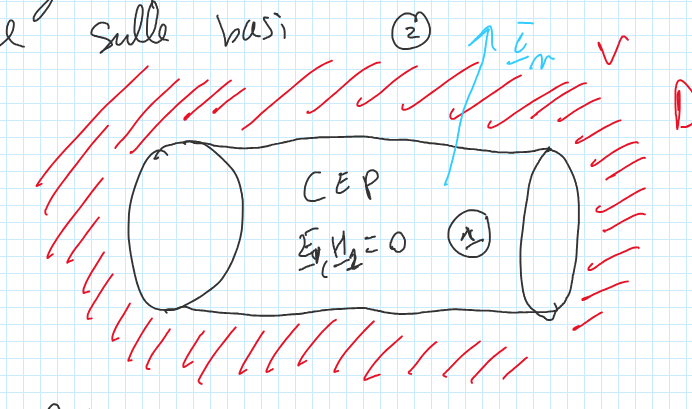
\includegraphics[width=0.75\linewidth]{Chapter_two/Chapt2img1.png}
        \end{figure}
        La superficie è orientata con normale $\underline{i}_{n}$. Lo spazio interno al CEP è segnato con (1), mentre quello esterno con
        (2). È di nostro interesse ricavare le equazioni di raccordo relative alla superficie laterale e alla base. Per le prime:
        \begin{equation}
            \label{eqn:raccordo_guida}
            \underline{i}_{n}\times (\underline{E}_{2}-\underline{E}_{1})\implies \underline{i}_{n}\times \underline{E}_{2}=\underline{i}_{n} \times \underline{E}_{1} = 0
        \end{equation}
        avendo sfruttato $\underline{E}_{1}=0$. Non possiamo utilizzare quella per il campo magnetico perché, seppur conosciamo $\underline{H}_{1}=0$ risulta:
        \begin{equation}
            \underline{i}_{n} \times (\underline{H}_{2}-\underline{H}_{1}) = \underline{J}_{S}
        \end{equation}
        Non conosciao l'espressione della corrente superficiale perché è indotta dal campo, dunque è un incognita del problema che 
        sarà nota solo quando lo saranno le sorgenti. Allora come condizione al raccordo utilizziamo la (\ref{eqn:raccordo_guida}). \\
        Mancano le condizioni alla base, che dipendono dal ricevente e dal trasmittente. Poiché è impensabile risolvere il problema elettromagnetico 
        per ogni possibile sorgente, scegliamo di non considerarle e trovare la soluzione generale del problema, che non avendo ancora informazioni su Rx e Tx ammette più soluzioni.
        Una volta trovata, aggiungiamo i generatori ed il carico per trovare la situazione unica. \\ \\
        Supponiamo ora di avere un mezzo normale ed omogeneo. In assenza di sorgenti impresse, di cui è responsabile il generatore che abbiamo staccato, le equazioni di Maxwell
        assumono la forma:
        \begin{equation}
            \begin{cases}
                \nabla \times \underline{E} = -j \omega \mu \underline{H} \\
                \nabla \times \underline{H} =j \omega \varepsilon \underline{E} \\
                \nabla \cdot (\varepsilon \underline{E}) = 0 \\
                \nabla \cdot (\mu\underline{H})
            \end{cases}
        \end{equation}
        Ipotizziamo inoltra che la struttura guidata sia \textbf{invariante per traslazione rispetto ad una direzione dello spazio}, ovvero
        che questa abbia \textbf{simmetria cilindrica}:
        \begin{figure}[h!]
            \center  
            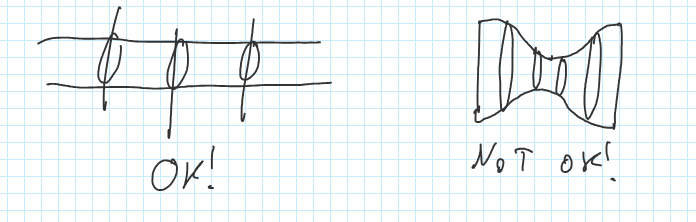
\includegraphics[width=0.75\linewidth]{Chapter_two/Chapt2img2.png}
        \end{figure} \\
        L'asse lungo la quale la guida ha simmetria cilindrica si chiama \textbf{asse z}. È sbagliato dire che
        è l'asse lungo la quale c'è la propagazione, seppur in futuro faremo vedere che è proprio così. \\
        Cerchiamo delle soluzioni particolari di campo. Faremo vedere che tutte le possibili soluzioni
        potranno essere scritte come combinazioni di queste. Tali soluzioni particolari sono classificate in base
        alle condizioni sulle componenti longitudinali di $\underline{E}$ ed $\underline{H}$:
        \begin{center}
            \begin{tabular}{|| c | c | c ||}
                \hline
                TE & TM & TEM \\
                 \hline
                $\begin{matrix} E_{z}=0 \\ H_{z} \neq 0 \end{matrix}$ &
                $\begin{matrix} E_{z} \neq 0 \\ H_{z} = 0 \end{matrix}$ &
                $\begin{matrix} E_{z}=0 \\ H_{z} = 0 \end{matrix}$  \\
                \hline
            \end{tabular}
        \end{center} \newpage
        Per capire di cosa si sta parlando, facciamo presente che nella nostra convenzione per le guide dìonda, la componente $z$ identifica una sezione della guida, mentre
        la coordinata $\underline{r}_{t}=(x,y)$ un punto sulla sezione:
        \begin{figure}[h!]
            \center 
            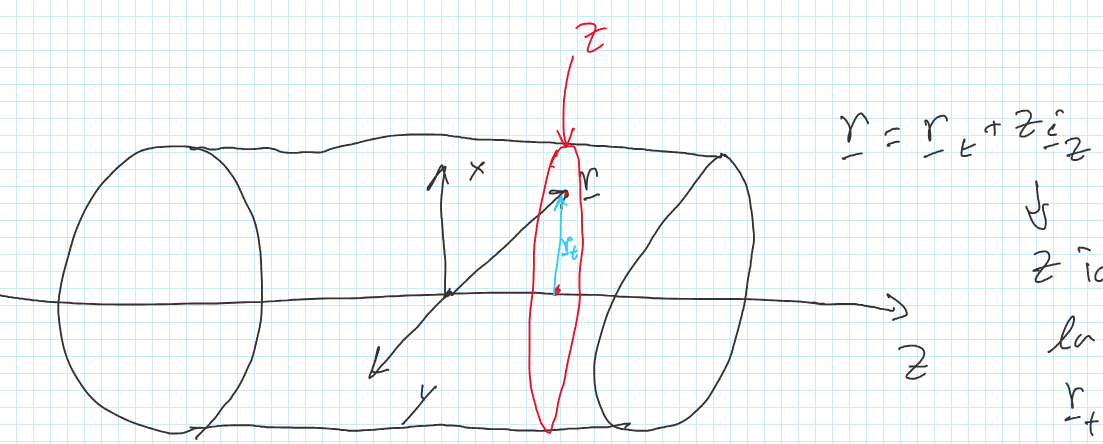
\includegraphics[width=0.75\linewidth]{Chapter_two/Chapt2img3.png}
        \end{figure} \\
        Alle tre soluzioni TE, TM e TEM, che stanno rispettivamente per Trasverso Elettrico, Magnetico ed ElettroMagnetico,
        sono associati i rispettivi modi TE, TM e TEM. Premesso che:
        \begin{equation}
            \underline{E} = \underline{E}_{t}+E_{z}\underline{i}_{z} \qquad \underline{H} = \underline{H}_{t}+H_{z}\underline{i}_{z}
        \end{equation}
        I modi corrispondono a soluzioni per cui l'espressione delle componenti longitudinali del campo 
        elettrico e magnetico si possono fattorizzare come il prodotto di una funzione scalare per una funzione vettoriale:
        \begin{equation}
            \label{eqn:fattorizzazione_modi}
            \begin{cases}
                \underline{E}_{t}(\underline{r}_{t},z)=V(z)\underline{e}(\underline{r}_{t}) \\
                \underline{H}_{t}(\underline{r}_{t},z)=I(z)\underline{h}(\underline{r}_{t})
            \end{cases}
        \end{equation}
        dove $V(z)$ e $I(z)$ sono dette \textbf{funzioni scalari di modo} e $\underline{e}(\underline{r}_{t})$ ed $\underline{h}(\underline{r}_{t})$ funzioni 
        vettoriali di modo. Per i modi TEM vedremo che $V(z)$ e $I(z)$ corrispondono a tensione e corrente, ma in generale non è vero.
    \section{Modi TEM}
    Quando fattorizziamo le funzioni scalari e vettoriali di modo sono definite a meno di una costante moltiplicativa, quindi non sono determinate.
    Apparentemente questo è un problema perché per le componenti trasversali dei campi abbiamo due equazioni in tre incognite ciascuna al posto delle due sole
    componenti trasversali.\\
    Per risolvere il problema utilizziamo le \textbf{equazioni di Markuvitz-Schwinger}, che sono nient'altro 
    che una riscrittura delle equazioni di Maxwell:
    \begin{equation}
        \label{eqn:eq_Markuvitz-Schwinger}
        \begin{cases}
            \displaystyle -\frac{\partial}{\partial t}\underline{E}_{t}=j \omega \mu [\underline{H}_{t}\times \underline{i}_{z}+\displaystyle \frac{1}{k^{2}}\nabla_{t}\nabla_{t}\cdot (\underline{H}_{z}) \times \underline{i}_{z}] \\
            \displaystyle - \frac{\partial}{\partial t}\underline{H}_{t}=j\omega \varepsilon [\underline{i}_{z} \times \underline{E}_{t}+ \displaystyle \frac{1}{k^{2}}\nabla_{t} \nabla_{t} \cdot (\underline{i}_{z} \times \underline{E}_{t})] \\
            j \omega \mu H_{z} = \nabla_{t} \cdot (\underline{i}_{z} \times \underline{E}_{t}) \\
            j \omega \varepsilon E_{z}=\nabla_{t}\cdot (\underline{H}_{t} \times \underline{i}_{z})
        \end{cases}
    \end{equation}
    dove $\nabla_{t} = \nabla - \frac{\partial}{\partial z} \underline{i}_{z}$ è il \textbf{nabla trasverso}, che agisce solo
    sulle componenti trasverse, mentre $k$ è la \textbf{costante di propagazione} e vale $k=\omega \sqrt{\varepsilon \mu}$, misurata in $m^{-1}$.
    \\ Le equazioni di Markuvitz-Schwinger separano la parte trasversa, che si trova  da sola nelle prime due equazioni, da quella longitudinale.
    Allora ci si ricava la parte trasversa e poi le longitudinali.
    In questa sezione cerchiamo le \textbf{soluzioni TEM}, dunque partiamo dal ricavarci l'espressione delle (\ref{eqn:eq_Markuvitz-Schwinger}) per questo caso particolare. Utilizziamo ultime due equazioni e sfruttiamo il fatto che le componenti longitudinali 
    $H_{z}$ ed $E_{z}$ sono nulle per i modi TEM:
    \begin{equation}
        \begin{cases}
            j \omega \mu H_{z} = \nabla_{t} \cdot (\underline{i}_{z} \times \underline{E}_{t})  \implies \nabla_{t} \cdot (\underline{i}_{z} \times \underline{E}_{t}) = 0 \\
            j \omega \varepsilon E_{z} = \nabla_{t} \cdot (\underline{H} \times \underline{i}_{z})  \implies \nabla_{t} \cdot (\underline{H} \times \underline{i}_{z}) = 0
        \end{cases}
    \end{equation}
    Sostituendo nella prima e seconda equazione di Markuvitz-Schwinger
    \begin{align}
        -\frac{\partial}{\partial t} \underline{E}_{t} = j \omega \mu [\underline{H}_{t} \times \underline{i}_{z} - \frac{1}{k^{2}}\nabla_{t}\nabla_{t}\cdot 0] = j \omega \mu(\underline{H}_{t} \times \underline{i}_{z}) \\
        -\frac{\partial}{\partial t} \underline{H}_{t} = j \omega \varepsilon [\underline{i}_{z}\times \underline{E}_{t}+\frac{1}{k^{2}}\nabla_{t}\nabla_{t} \cdot 0] = j \omega \varepsilon (\underline{i}_{z} \times \underline{E}_{t})
    \end{align}
    In sintesi, per i modi TEM, le equazioni di Markuvitz-Schwinger hanno questa forma:
    \begin{equation}
        \label{eqn:MS_TEM}
        \begin{cases}
            -\frac{\partial}{\partial t}\underline{E}_{t} = j \omega \mu (\underline{H}_{t} \times \underline{i}_{z}) \\
            -\frac{\partial}{\partial t} \underline{H}_{t} = j \omega \varepsilon (\underline{i}_{z} \times \underline{E}_{t}) \\
            \nabla_{t} \cdot (\underline{i}_{z} \times \underline{E}_{t}) = 0 \\
            \nabla_{t} \cdot (\underline{H}_{t} \times \underline{i}_{z}) = 0
        \end{cases}
    \end{equation}
    Fatto ciò, sostituiamo le espressioni fattorizzate (\ref{eqn:fattorizzazione_modi}) nella prima equazione delle (\ref{eqn:MS_TEM}):
    \begin{equation}
        -\frac{\partial}{\partial t}(V(z)\underline{e}(\underline{r}_{t})) = - \underline{e}(\underline{r}_{t})V(z) = j \omega \mu I(z)\underline{h}(\underline{r}_{t}) \times \underline{i}_{z}
    \end{equation}
    tenendo a mente che nella derivata del prodotto quella di $V(z)$ rispetto a $t$ è nulla, perché indipendente dalle componenti trasversali.
    Manipoliamo l'espressione dividendo per $j \omega \mu$ ottenendo:
    \begin{equation}
        \label{eqn:mi_serve}
        \underline{e}(\underline{r}_{t}) \cdot [-\frac{\displaystyle \frac{dV}{dz}}{j \omega \mu I(z)}] = \underline{e}(\underline{r}_{t}) \cdot \frac{1}{A}= \underline{h}(\underline{r}_{t}) \times \underline{i}_{z}
    \end{equation}
    avendo posto:
    \begin{equation}
         A = -\frac{\displaystyle \frac{dV}{dz}}{j \omega \mu I(z)}
    \end{equation}
    Sotto l'ipotesi di mezzo omogeneo $\mu$ non dipende dallo spazio e quindi, apparentemente, $A$ soltanto da $z$. Ma se osserviamo
    la relazione (\ref{eqn:mi_serve}), notiamo che il secondo membro dipende soltanto dalle coordinate trasversali, per cui la relazione per valere deve 
    dipendere anche a sinistra solo da $\underline{r}_{t}$.
    Condensando il tutto, otteniamo la \textbf{prima equazione dei telegrafisti}\footnote{È solo il primo pezzo, il secondo è una conseguenza di Markuvitz-Schwinger così come il primo}:
    \begin{equation}
        \label{eqn:prima_eq_telegrafisti}
        \begin{cases}
            \displaystyle \frac{dV}{dz} = \frac{j \omega \mu I}{A} \\
            \underline{e}(\underline{r}_{t}) = A \underline{h}(\underline{r}_{t}) \times \underline{i}_{z}
        \end{cases}
    \end{equation}
    Inoltre $\underline{e}$ è ricavabile da $\underline{h}$ e viceversa. Manipoliamo 
    il secondo pezzo dell'equazione dei telegrafisti premoltiplicando vettorialmente per $\underline{i}_{z}$:
    \begin{equation}
        \underline{i}_{z} \times \underline{e} = A \underline{i}_{z}(\underline{h} \times \underline{i}_{z}) = A (\underline{i}_{z} \times \underline{h}) \times \underline{i}_{z}
    \end{equation}
    Utilizziamo l'identità vettoriale notevole:
    \begin{equation}
        = A [(\underline{i}_{z} \cdot \underline{i}_{z})\underline{h}-(\underline{h}\cdot \underline{i}_{z})\underline{i}_{z}]
        = A[|\underline{i}_{z}|^{2}\underline{h}-0] = A\underline{h}
    \end{equation}
    dove abbiamo sfruttato il fatto che $\underline{h} \cdot \underline{i}_{z} = 0$.\footnote{perché $\underline{h}$ è totalmente trasversale}
    In definitiva la relazione fra la componente longitudinale di $\underline{e}$ ed $\underline{h}$ è:
    \begin{equation}
        \label{eqn:mi_serve2}
        \underline{i}_{z} \times \underline{e} = A \underline{h}
    \end{equation}
    Per la seconda equazione di Markuvitz-Schwinger il procedimento è analogo a quello fatto finora: sostituiamo l'espressione fattorizzata nella
    seconda equazione e ricaviamo:
    \begin{equation}
        -\underline{h}(\underline{r}_{t}) \frac{d}{dz}I(z)= j \omega \varepsilon V(z) \underline{i}_{t} \times \underline{e}(\underline{r}_{t})
    \end{equation}
    sostituendo la (\ref{eqn:mi_serve2}) che abbiamo appena ricavato
    \begin{equation}
        \implies -\underline{h}(\underline{r}_{t}) \frac{d}{dz}I(z) = j \omega AV(z)\underline{h}(\underline{r}_{t})
        \implies [\frac{d}{dz}I(z)+j\omega \varepsilon A V(z)]\underline{h} = 0
    \end{equation}
    poiché a noi non interessano le soluzioni banali per $\underline{h} = 0$, l'espressione è nulla se è nullo l'altro termine del prodotto, da
    cui otteniamo la \textbf{seconda equazione dei telegrafisti}:
    \begin{equation}
        -\frac{d}{dz}I(z) = j \omega A V(z)
    \end{equation}

    Non ci resta che determinare $\underline{e}$ ed $\underline{h}$. Sfruttiamo la terza equazione di Markuvitz-Schwinger
    e sostituiamo l'espressione fattorizzata:
    \begin{equation}
        0 = \nabla_{t} (\underline{i}_{z} \times \underline{E}_{t})= V(z)\nabla_{t} \cdot (\underline{i}_{z} \times \underline{e}) = V(z) \nabla_{t} \cdot(A\underline{h})
    \end{equation}
    Se $A=0$ oppure $V(z)=0$ c'è la soluzione banale, dunque non ci interessa. Ricaviamo allora:
    \begin{equation}
        \nabla_{t} \cdot \underline{h} = 0
    \end{equation}
    ovvero che $\underline{h}$ è un campo indivergente. Se però esprimiamo la terza equazione come identità notevole:
    \begin{equation}
        0 = \nabla_{t} \cdot (\underline{i}_{z} \times \underline{E}_{t}) =V(z)[(\nabla_{t} \times \underline{i}_{z})\underline{e} - \underline{i}_{z} \cdot \nabla_{t} \times \underline{e}] = 0
    \end{equation}
    ma $\nabla_{t} \times \underline{i}_{z}$ perché $\underline{i}_{z}$ è un versore e non dipende da $t$. Inoltre $V(z)$ si può cancellare ambo membri ottenendo:
    \begin{equation}
        \underline{i}_{z} \cdot \nabla_{t} \times \underline{e} = 0
    \end{equation}
    cioè che il rotore di $\underline{e}$ è perpendicolare all'asse $z$. Calcolando il rotore di $\underline{e}$:
    \begin{equation}
        \nabla_{t} \times \underline{e} = 
        \begin{vmatrix} 
            \underline{i}_{x} & \underline{i}_{y} & \underline{i}_{z} \\
            \displaystyle \frac{\partial}{\partial x} & \displaystyle \frac{\partial}{\partial y} & 0 \\
            e_{x} & e_{y} & 0
        \end{vmatrix} = \underline{i}_{z} \cdot (\frac{\partial}{\partial x}e_{y}-\frac{\partial}{\partial y}e_{x}) = 0
    \end{equation}
    cioè il rotore dipende solo dalla componente longitudinale, che è nulla, per cui il rotore è di $\underline{e}$ è nullo. 
    Allora $\underline{e}$ è un campo irrotazionale. Facendo gli stessi calcoli con la quarta equazione di Markuvitz-Scwhinger si ricava che $\underline{h}$ è irrotazionale
    ed $\underline{e}$ è indivergente. IN definitiva otteniamo
    \begin{equation}
        \label{eqn:campi_irrotazionali_indivergenti_TEM}
        \begin{cases}
            \nabla \cdot \underline{e} = 0 \qquad \nabla \times \underline{e} = 0
            \\ \nabla \cdot \underline{h} = 0 \qquad \nabla \times \underline{h} = 0
        \end{cases}
    \end{equation}
    che equivale a dire che $\underline{e}$ ed $\underline{h}$ sono \textbf{campi armonici}.\footnote{ovvero sia indivergenti che irrotazionali}
    \\ \\
    Il fatto che $\underline{e}$ ed $\underline{h}$ siano armonici ci porta a pensare che potrebbero avere un potenziale scalare, questo 
    perché un campo irrotazionale è anche conservativo se è semplicemente connesso\footnote{cioè se si può deformare nel dominio una curva con continuità senza uscire dal dominio}
    Già considerando la sezione di un cavo coassiale, ci si rende conto che non è un domino semplciemente connesso (per verificarlo basta prendere una curva che circonda l'anima 
    e comprimerla, uscirà fuori dal dominio dove è interposto il dielettrico).
    \newpage
    \begin{figure}[h!]
        \center 
        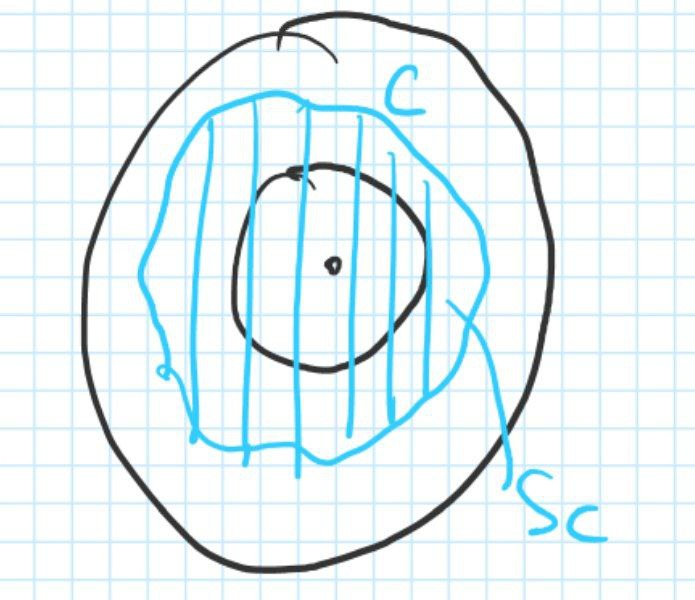
\includegraphics[width=0.5\linewidth]{Chapter_two/Chapt2img6.png}
    \end{figure} 
    Tuttavia, se $C$ è una curva che sta nel dominio identificato tra l'anima (il cerchio in mezzo) e la calza
    (il cerchio esterno) ed $S_{c}$ la superficie che ha $C$ come bordo, possiamo applicare la prima legge di Maxwell:
    \begin{equation}
        \oint_{C} \underline{E} \cdot \underline{i}_{n}dS = j \omega \mu \iint_{S_{C}}\underline{H}\cdot \underline{i}_{n}dS
    \end{equation}
    Per la sezione del cavo coassiale, così come per tutte le guide d'onda, la normale alla superficie $S_{c}$ è l'asse $z$, dunque $\underline{i}_{n}=\underline{i}_{z}$.
    Per cui $\underline{H} \cdot \underline{i}_{z}=H_{z}$, che è nulla per i modi TEM. Allora:
    \begin{equation}
        \oint_{C} \underline{E} \cdot \underline{i}_{n}dS = j \omega \mu \iiint_{S_{C}} \underline{H} \cdot \underline{i}_{z} dS = 0
    \end{equation}
    che è proprio la definizione di campo conservativo. In sintesi, per i modi TEM il campo elettrico è conservativo.
    \section{Caratterizzazione delle guide d'onda}
        In un problema elettromagnetico, i campi incogniti sono $\underline{E}(\underline{r}_{t}, z)$ ed $\underline{H}(\underline{r}_{t}, z)$.
        Per i modi TEM risulta:
        \begin{equation}
            \begin{cases}
                \underline{E}_{t}(\underline{r}_{t},z)=V(z)\underline{e}(\underline{r}_{t}) \\
                \underline{H}_{t}(\underline{r}_{t},z)=I(z)\underline{h}(\underline{r}_{t})
            \end{cases}
        \end{equation}
        con $V(z)$ ed $I(z)$ tensione e corrente in corrispondenza della coordinata $z$. Una volta noti $\underline{e}(\underline{r}_{t}, t)$
        ed $\underline{h}(\underline{r}_{t},z)$ occorre ricavare $V(z)$ ed $I(z)$. Partiamo da due equazioni che legano tensioni e corrente:
        \begin{equation}
            \label{eqn:eq_tensione_corrente}
            \begin{cases}
                \frac{d}{dz}V(z)=-j k Z_{0}I(z) \\
                \frac{d}{dz}I(z) = -j \displaystyle \frac{k}{Z_{0}}V(z)
            \end{cases}
        \end{equation}
        dove $k$ è la costante di propagazione e $Z_{0}$ l'impedenza caratteristica della linea:
        \begin{equation}
            \begin{cases}
                Z_{0} = \displaystyle \frac{1}{A} \sqrt{\frac{\mu}{\varepsilon}} \\
                K(\omega)= \omega \sqrt{\varepsilon \mu}
            \end{cases}
        \end{equation}
        dove $A$ è una certa costante\footnote{serve solo ad evidenziare che l'impedenza caratteristica è proporzionale alla radice del rapporto
        fra permittività elettrica e permeabilità magnetica}. In generale la costante di propagazione è un numero complesso $K=\beta -j \alpha$. Quando
        avremo bisogno di ipotizzare che $k \in \mathbb{R}$, scriveremo semplicemente $k=\beta$. \\
        Ipotizziamo che $Z_{0}$ e $k$ siano reali. Per un mezzo omogeneo troviamo la soluzione generale di $V(z)$ ed $I(z)$ risolvendo il sistema
        (\ref{eqn:eq_tensione_corrente}). Derivando in $z$ la prima equazione:
        \begin{equation}
            \frac{d^{2}}{dz^{2}}V(z)=-jkZ_{0}\frac{d}{dz}I(z)=-jkZ_{0}(-j\frac{k}{Z_{0}}V(z))= -k^{2}V(z)
        \end{equation}
        ottenendo un equazione analoga a quella di un oscillatore armonico:
        \begin{equation}
            \frac{d^{2}}{dz^{2}}V(z)+k^{2}V(z)=0
        \end{equation}
        la quale avrà integrale generale:
        \begin{equation}
            \label{eqn:prima_exp_V}
            V(z)=V^{+}e^{-j k z}+V^{-}e^{jkz}=V^{+}(z)+V^{-}(z) \qquad V^{+},V^{-} \in \mathbb{C}
        \end{equation}
        La (\ref{eqn:prima_exp_V}) è scritta come somma di due termini: un'onda \textbf{progressiva} con coefficiente
        $V^{+}$ ed una \textbf{regressiva} con coefficiente $V^{-}$. Per interpretarne il significato fisico, torniamo nel dominio 
        del tempo ricavando l'espressione dell'onda progressiva:
        \begin{align}
            v(z, t)= \Re[V^{+}(z)e^{j \omega t}] = \Re(V^{+}e^{-jkz}e^{j \omega t}) =
            \\ \Re[|V^{+}|e^{j \varphi_{v} ^{+}}e^{-j k z}e^{j \omega t}] = |V^{+}|\cos(\omega t-kz+\varphi^{+}_{v})
        \end{align}
        Assumendo $\varphi^{+}_{v} = 0$, un'onda progressiva ha la forma:
        \begin{equation}
            \label{eqn:eq_onda_prog}
            V^{+}(z, t) = |V^{+}|\cos(\omega t-kz)
        \end{equation}
        Fissato $t=0$\footnote{Vale $\forall t$ a meno di un contributo di fase} e sfruttando $k=\beta$ otteniamo nello spazio una cosinusoide:
        \begin{equation}
            V^{+}(z)=|V^{+}|\cos(\beta z)
        \end{equation}
        la quale ha periodo $\displaystyle \lambda = \frac{2 \pi}{\beta}$, che è la \textbf{lunghezza d'onda}. Si noti che
        è stato possibile definire la lunghezza d'onda perché $k$ è reale, ma tutte le altre considerazioni hanno valore generale.
        \newpage
        Riscrivendo la (\ref{eqn:eq_onda_prog}):
        \begin{equation}
            V^{+}(z)=|V^{+}|\cos{(\beta (z - \frac{\omega}{\beta}))t}
        \end{equation}
        Facendo un'nalisi dimensionale:
        \begin{equation}
            [\frac{\omega}{\beta} = \frac{\omega}{\omega \sqrt{\varepsilon \mu}}] = [\frac{1}{\sqrt{\varepsilon \mu}}] = m/s
        \end{equation}
        dunque $\omega/\beta=v$ è una velocità, per cui:
        \begin{equation}
            V^{+}(z)=|V^{+}|\cos(\beta(z-vt)) = f(z-vt)
        \end{equation}
        Graficamente, se la funzione $f$ viene traslata di $\Delta t$, l'onda sarà traslata di $v \Delta t$ in avanti. Da qui
        la definizione di onda progressiva: è un'onda che si propaga nella direzione delle $z$ positive.
        Se $k \in \mathbb{C}$, cioè se ci sono perdite, sostituendo $k=\beta-j\alpha$ nell'espressione di prima:
        \begin{equation}
            V^{+}(z,t)=\Re[|V^{+}|e^{j \varphi_{v} ^{+}}e^{-j \beta z}e^{-\alpha z}e^{j \omega t}]= |V^{+}|e^{-\alpha z}\cos(\beta z-\omega t)
        \end{equation}
        otteniamo un'espressione identica a prima a meno di un fattore di attenuazione $e^{-\alpha z}$, il quale rappresenta le perdite del mezzo. In sintesi,
        un mezzo reale con perdite ha parte immaginaria non nulla che più è grande più attenua la propagazione. Questa cosa è vera solo se $\beta$ è lineare con $\omega$.
        \\ 
        Per le onde regressive il ragionamento è identico e si ottiene:
        \begin{equation}
            V^{-}(z,t)=|V^{-}|\cos(\beta(+vt))=f(z+vt)
        \end{equation}
        da cui la definizione di onda regressiva: è un'onda che si muove nella direzione negativa dell'asse $z$.
        \\ \\
        Finora abbiamo trattato la soluzione  in tensione, ma a noi occorre anche quella in corrente. Conoscendo
        $V(z)$ possiamo sostituire la (\ref{eqn:prima_exp_V}) nella (\ref{eqn:eq_tensione_corrente}):
        \begin{equation}
            \frac{d}{dz}V(z)=-jkZ_{0}I(z) \implies I(z)=\frac{j}{kZ_{0}}\frac{d}{dz}V(z)
        \end{equation}
        \begin{equation}
            = \frac{j}{kZ_{0}}[-j k V^{+}e^{-jkz}+jkV^{-}e^{jkz}] = \frac{V^{+}}{Z_{0}}e^{-jkz}-\frac{V^{-}}{Z_{0}}e^{jkz}
        \end{equation}
        \begin{equation}
            = \frac{V^{+}(z)}{Z_{0}}+(-\frac{V^{-}(z)}{Z_{0}})=I^{+}(z)+I^{-}(z)
        \end{equation}
        In definitiva, per risolvere il problema elettromagnetico in questo caso basta trovare le due costanti  $V^{+}$ e $V^{-}$, ammesso che si conosca 
        $k$ ed $\omega$. Una soluzione di questo tipo si chiama \textbf{ad onda viaggiante}.
        La stessa soluzione si può esprimere nella \textbf{rappresentazione di onda stazionaria}, cioè tramite seni e coseni.
        \begin{equation}
            V(z)=V^{+}e^{-jkz}+V^{-}e^{jkz}=V^{+}(\cos(kz)-j\sin(kz))+V^{-}(\cos(kz)+j\sin(kz))
        \end{equation}
        \begin{equation}
            =(V^{+}+V^{-})\cos(kz)-j(V^{+}-V^{-})\sin(kz)
        \end{equation}
        Notiamo che:
        \begin{align}
            I(0)=\frac{V^{+}}{Z_{0}}e^{0}-\frac{V^{-}}{Z_{0}e^{0}} \implies V^{+}-V^{-}=Z_{0}I(0) \\
            V(0)=V^{+}e^{0}+V^{-}e^{0}=V^{+}+V^{-}
        \end{align}
        dunque:
        \begin{equation}
            V(z)=V(0)\cos(kz)-jZ_{0}I(0)\sin(kz)
        \end{equation}
        e a noi questa cosa piace perché vuol dire che conoscendo corrente e tensione all'inizio della linea, cioè per
        $z=0$, possiamo conoscerne il valore ovunque sulla stessa linea. Tramite lo 
        stesso procedimento ricaviamo un'espressione simile per la corrente, ottenendo le \textbf{formule del trasporto}:
        \begin{equation}
            \begin{cases}
                \displaystyle I(z) = I(0)\cos(kz)-j\frac{V(0)}{Z_{0}}\sin(kz) \\
                V(z) = V(0)\cos(kz)-jZ_{0}I(0)\sin(kz)
            \end{cases}
        \end{equation}
        \\ 
        A livello circuitale, una linea di trasmissione è rappresentata da una coppia di rettangoli, il cui 
        spessore sottolinea il fatto che c'è fenomeno propagativo. Una linea di trasmissione è caratterizzata dalla sua lunghezza $l$,
        la sua costante di propagazione $k$ e l'impedenza caratteristica $Z_{0}$. 
        \begin{figure}[h!]
            \center  
            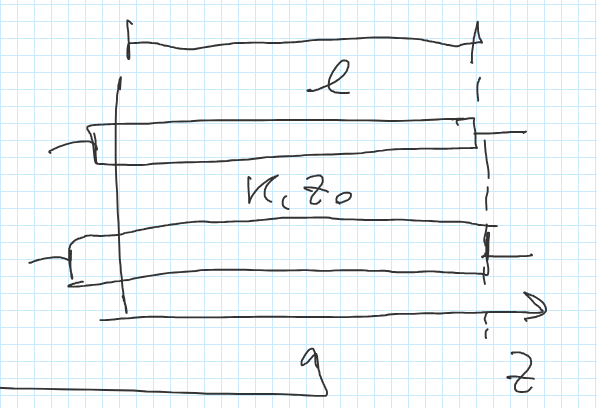
\includegraphics[width=0.75\linewidth]{Chapter_two/Chapt2img4.png}
        \end{figure}
        \\
        Tensione e corrente sono funzioni periodiche di $\lambda$, dunque ci aspettiamo che l'impedenza lungo la linea sia anch'essa 
        una funzione periodica:
        \begin{equation}
            Z(z) = \frac{V(z)}{I(z)} = \frac{\displaystyle I(z) = I(0)\cos(kz)-j\frac{V(0)}{Z_{0}}\sin(kz)}{V(z) = V(0)\cos(kz)-jZ_{0}I(0)\sin(kz)}
        \end{equation}
        Raccogliendo $I(0)\cos(kz)$ sia a numeratore che denominatore otteniamo:
        \begin{equation}
            \label{eqn:trasporto_impedenza}
            Z(z)=\displaystyle \frac{\displaystyle \frac{V(0)}{I(0)}-jZ_{0}\tan(kz)}{1-\displaystyle \frac{V(0)}{I(0)}\frac{1}{Z_{0}}\tan(kz)} = 
            \frac{Z(0)-jZ_{0}\tan(kz)}{\displaystyle Z_{0}-Z(0)\tan(kz)}\cdot Z_{0}
        \end{equation}
        dove $Z(0)$ è l'impedenza valutata all'inizio della linea. Nella pratica è comodo utilizzare la
        (\ref{eqn:trasporto_impedenza}) per $z=-d$, cioè per distanze negative, perché la tangente viene con il segno positivo\footnote{e le arcotangenti sono immediate da calcolare}.
        Per l'ammettenza:
        \begin{equation}
            Y(z)=\frac{Y_{0}-Y(0)\tan(kz)}{Y(0)-Y_{0}\tan(kz)}
        \end{equation}
        avendo posto $Y(0)=1/Z(0)$ e $Y_{0}=1/Z_{0}$. Sia l'ammettenza che l'impedenza sono periodiche di $\lambda/2$, perché
        sono espresse tramite $\tan(kz)$. \\
        Un altro parametro significativo delle linee di trasmissione è il \textbf{coefficiente di riflessione} $\Gamma$:
        \begin{equation}
            \Gamma (z) = \frac{V^{-}(z)}{V^{+}(z)} = \frac{V^{-}}{V^{+}}\exp(j2kz)
        \end{equation}
        definito come il rapporto fra l'onda regressiva e quella progressiva. Può essere definito anche in corrente, differendo dalla
        definizione in tensione di un segno meno. Il coefficiente di riflessione ha significato fisico: quantifica di quanto l'onda che si 
        propaga sulla linea viene riflessa in corrispondenza della coordinata $z$. Notiamo che:
        \begin{equation}
            \Gamma(0)=\frac{V^{+}}{V^{-}} \implies \Gamma(z) = \Gamma(0)\exp(j2kz)
        \end{equation}
        Il coefficiente di riflessione ha lo stesso periodo $\lambda/2$ che ha pure l'impedenza. Queste due 
        infatti sono legate:
        \begin{equation}
            Z(z)=\frac{V(z)}{I(z)}=\displaystyle \frac{V^{+}(z)+V^{-}(z)}{\displaystyle \frac{V^{+}}{Z_{0}}-\frac{V^{-}}{Z_{0}}}
            = Z_{0}\frac{V^{+}(z)}{V^{+}(z)}[\frac{1+\Gamma(z)}{1-\Gamma(z)}] = \frac{1+\Gamma(z)}{1-\Gamma(z)} 
        \end{equation}
        Viceversa:
        \begin{equation}
            \Gamma(z)=\frac{Z(z)-Z_{0}}{Z(z)+Z_{0}} = \frac{Y(0)-Y(z)}{Y(0)+Y(z)}
        \end{equation}
        \begin{equation}
            Y(z)=\frac{1-\Gamma(z)}{1+\Gamma(z)}
        \end{equation}
        Se la rete è senza perdite e dunque $k=\beta$, il coefficiente di riflessione vale:
        \begin{equation}
            \Gamma (z)=\Gamma (0)\exp(2 \beta z) \implies \begin{cases}
                |\Gamma(z)|=|\Gamma(0)| \\
                \angle \Gamma(z) = 2 \beta z
            \end{cases}
        \end{equation}
        cioè il modulo è costante e la fase è lineare in $z$, per cui nel piano complesso descrive una circonferenza. Poiché 
        il modulo non può essere negativo e l'onda riflessa può essere al massimo pari a quella propagata:
        \begin{equation}
            0 \leq \Gamma(z) \leq 1
        \end{equation}
        È utile esprimere, per il futuro, i termini di coefficiente di riflessione i valori di
        tensione e corrente:
        \begin{align}
            \label{eqn:eq_VI_Gamma}
            V(z)=V^{+}(z)+V^{-}(z)=V^{+}(1+\Gamma (z))  \\
            I(z)=I^{+}(z)+I^{-}(z)=I^{+}(z)(1-\Gamma (z))
        \end{align}
        \\ Definiamo ora la potenza attraverso una sezione\footnote{Qui per la potenza media $\overline{P}$ ho messo il cappello, che non ho messo in precedenza. Da qua in poi sarà sempre segnata col cappello.}:
        \begin{equation}
            P(z)=\frac{1}{2}V(z)I^{*}(z) = \overline{P}+jQ(z)
        \end{equation}
        \begin{figure}[h!]
            \center  
            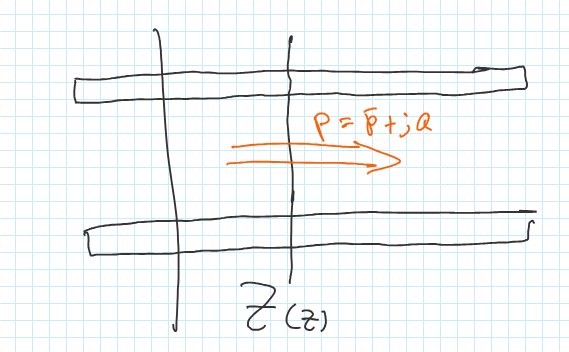
\includegraphics[width=0.75\linewidth]{Chapter_two/Chapt2img5.png}
        \end{figure}
        La potenza media attraverso la superficie del dominio è data dal flusso del vettore di Poynting, dunque $\overline{P}$ è 
        la potenza che attraversa la sezione\footnote{L'area identificata dall'intersezione tra il piano dei punti di longitudine $z$ e la guida d'onda} alla longitudine $z$. Similmente, $Q$ è la potenza reattiva che attraversa la sezione alla longitudine $z$.
         \newpage
        Consideriamo ora una linea di trasmissione ed il suo equivalente fisico:
        \begin{figure}
            \center 
            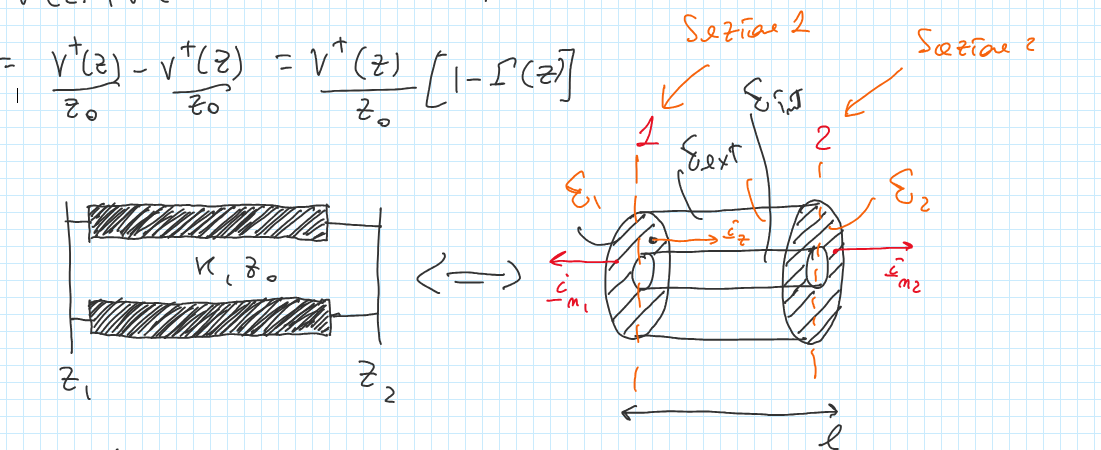
\includegraphics[width=0.75\linewidth]{Chapter_two/Chapt2img7.png}
        \end{figure}
        Stiamo considerando, in particolare, un cavo coassiale, ma le stesse considerazioni valgono
        per qualsiasi linea di trasmissione. Chiamiamo $\Sigma_{1}$ e $\Sigma_{2}$ le superfici delle "basi" del cilindro,
        orientate rispettivamente con $\underline{i}_{n1}$ ed $\underline{i}_{n2}$, $\Sigma_{int}$ la superficie laterale del cilindro interno,
        che corrisponde all'anima del cavo coassiale, e $\Sigma_{ext}$ la superficie laterale del cilindro esterno.
        Allora applichiamo Poynting alla superficie data dall'unione di queste quattro. Il flusso attraverso le due superfici laterali è nullo,
        perché stiamo considerando un conduttore elettrico perfetto. In virtù del fatto che $\underline{i}_{n1}=-\underline{i}_{n}$ e 
        $\underline{i}_{n2}=\underline{i}_{n}$, per come le abbiamo scelte, risulta:
        \begin{equation}
            \label{eqn:mi_serve3}
            \Phi(\underline{S}) = \Phi(\underline{S})_{\Sigma_{2}}-\Phi(\underline{S})_{\Sigma_{2}}
        \end{equation}
        Per la parte reale:
        \begin{equation}
            \Re[\Phi(\underline{S})]+\frac{\varepsilon '' \omega}{2}\iiint_{V} |\underline{E}|^{2}dV+\frac{\mu '' \omega}{2} \iiint_{V} |\underline{H}|^{2}dV
            +\frac{\sigma}{2}\iiint_{V}|\underline{E}|dV = - P_{g}
        \end{equation}
        dove $P_{g}$ è la potenza fornita dalle sorgenti interne. Nel nostro caso, sorgenti interne non ce ne sono e $\sigma, \mu'', \varepsilon'' = 0$ perché
        supponiamo che non ci siano perdite, ottenendo:
        \begin{equation}
            \Re[\Phi(\underline{S})]=0
        \end{equation}
        Dalla (\ref{eqn:mi_serve3}) risulta:
        \begin{equation}
            \Re[\Phi(\underline{S})] = \Re[\iint_{\Sigma_{2}} \frac{1}{2}\underline{H} \times \underline{E}\cdot \underline{i}_{n}
            -\iint_{\Sigma_{1}} \frac{1}{2}\underline{H} \times \underline{E}\cdot \underline{i}_{n}] = 0
        \end{equation}
        Ma la parte reale del flusso del vettore di Poynting è la potenza attiva media, per cui:
        \begin{equation}
            P(z_{2})-P(z_{1}) = 0 \implies P(z_{2})=P(z_{1})
        \end{equation}
        cioè per una rete senza perdite e senza sorgenti interne la potenza media si conserva.
        \\ La stessa cosa non vale per la potenza reattiva. Infatti:
        \begin{equation}
            \textrm{Im}(\Phi(\underline{S})) +2 \omega \textrm{Im}[\iiint_{V} \overline{W}_{m}-\overline{W}_{e}] = - \textrm{Im}(-P_{g}) = 0
        \end{equation}
        ovvero:
        \begin{equation}
            Q(z_{2})-Q(z_{1})=2 \omega (\overline{W}_{m}-\overline{W}_{e})
        \end{equation}
        che generalmente è una quantità diversa da zero. In altre parole, la varizione del flusso di potenza reattiva
        dipende dal dislivello di energia elettrica e magnetica.
        \\ 
        È utile esprimere la potenza complessa in altre forme per ricavare risultati interessanti. In termini 
        di tensione e ammettenza oppure corrente e impedenza:
        \begin{align}
            P = \frac{1}{2}Z(z)|I(z)|^{2} \\
            P= \frac{1}{2}Y(z)|V(z)|^{2}
        \end{align}
        Oppure esprimendo tensioni e corrente tramite coefficiente di riflessione (\ref{eqn:eq_VI_Gamma}):
        \begin{equation}
            P(z)=\frac{1}{2}\frac{|V^{+}|^{2}}{Z_{0}} (1+\Gamma(z)-\Gamma(z)^{*}-|\Gamma(z)|^{2})
        \end{equation}
        Ipotizziamo che l'impedenza sia reale, ma tutto ciò è generalizzabile. In una linea senza perdite il modulo di $\Gamma(z) = \Gamma$ è costante, mentre la differenza fra un numero complesso e 
        la sua parte immaginaria ritorna $2j\textrm{Im}(z)$, per cui si può scrivere:
        \begin{equation}
            \label{eqn:potenza_attiva}
            P(z)=\frac{1}{2}\frac{|V^{+}|^{2}}{Z_{0}}(1+2j\textrm{Im}(\Gamma(z))-|\Gamma|^{2}) =
            P^{+}(1+2j\Gamma (z)-|\Gamma|^{2})
        \end{equation}
        Per capire il significato dell'espressione di sopra, ipotizziamo di avere solo onda progressiva. La potenza
        sarà:
        \begin{equation}
            P(z)= \frac{1}{2}V^{+}(z)(I^{+}(z))^{*} = \frac{1}{2}\frac{|V^{+}|^{2}}{Z_{0}}=P^{+}
        \end{equation}
        La parte reale della (\ref{eqn:potenza_attiva}):
        \begin{equation} 
            \label{eqn:mi_serve4}
            \Re[P(z)]=P^{+}-|\Gamma|^{2}P^{+} = P^{+}-P^{-}
        \end{equation}
        È la differenza fra la potenza in ingresso e quella riflessa, che è data dal prodotto fra il modulo quadro 
        del coefficiente di riflessione\footnote{La potenza va con il quadrato, perché si riflette la tensione al quadrato} e
        la parte reale della potenza.
        Il termine immaginario ci dice quanta potenza reattiva fluisce alla longitudine $z$. \\
        La (\ref{eqn:mi_serve4}) assume pienamente senso calcolando la potenza associata ad un'onda puramente regressiva:
        \begin{equation}
            P^{-}=\frac{1}{2}V^{-}(I^{-})^{*}=-\frac{1}{2}\frac{|V^{-}|^{2}}{Z_{0}} = 
            -\frac{1}{2Z_{0}}|\Gamma V^{+}|^{2} = - P^{+}|\Gamma|^{2}
        \end{equation}
        \\ Esprimiamo ora l'impedenza come somma di resistenza e reattanza:
        \begin{equation}
            P(z)=\frac{1}{2}Z(z)|I(z)|^{2} = \frac{1}{2}R(z)|I(z)|^{2}+j\frac{X(z)}{2}|I(z)|^{2}
        \end{equation}
        od in intermini di conduttanza e suscettanza:
        \begin{equation}
            P(z)=\frac{1}{2}G(z)|V(z)|^{2}+j\frac{1}{2}B(z)|V(z)|^{2}
        \end{equation}
        Da queste relazioni si evince che, visto che la potenza media si conserva, se c'è resistenza nulla in un punto non c'è flusso 
        di potenza attiva in nessun punto. Viceversa, la resistenza non può annullarsi se c'è flusso di potenza almeno in un punto.
    \section{Risoluzione elementare di linee di trasmissione omogenee}
        Consideriamo in questa sezione solo linee di trasmissione omogenee, cioè con le stesse grandezze 
        caratteristiche su tutta la linea. In seguito vedremo quelle non omogenee, cioè composte da più linee diverse.
        Per risolvere il problema elettromagnetico per le linee di trasmissione occorre ricavare i parametri
        $V^{+}$ e $V^{-}$. Tali parametri sono univocamente determinati dal generatore e dall'impedenza.
        Per risolvere gli esercizi sposteremo l'origine di continuo per facilitare il calcolo tramite le equazioni di trasporto.
        Questo non ci da problemi finché si tiene traccia di cosa stiamo calcolando: se per esempio calcoliamo l'impedenza all'ingresso e 
        continuiamo a chiamarla $Z(0)$ faremo inevitabilmente casino in altri sistemi di riferimento, per cui è buona norma dagli 
        nomi "unici". \\
        Consideriamo una generica linea di trasmissione:
        \begin{figure}[h!]
            \center 
            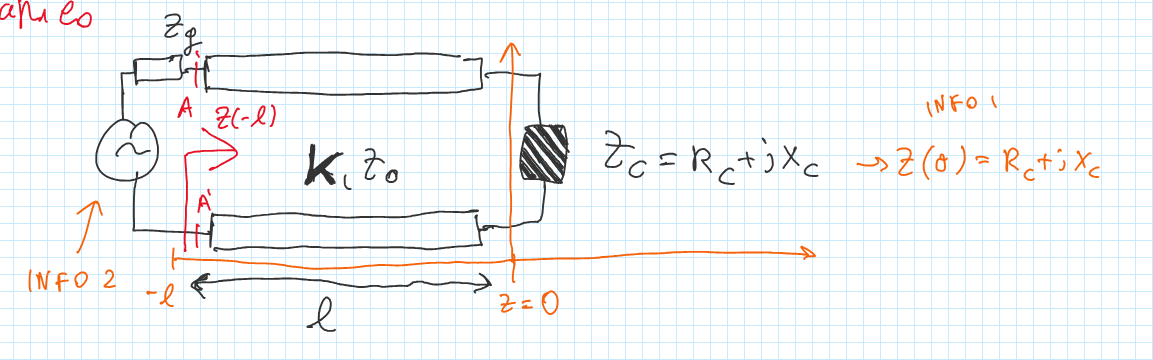
\includegraphics[width=0.75\linewidth]{Chapter_two/Chapt2img8.png}
        \end{figure}
        \\ Conosciamo l'impedenza di carico $Z_{C}$, indi per cui è conveniente posizionare l'origine in corrispondenza
        in corrispondenza della sezione finale, quella "vista" dall'impedenza $Z_{C}$. A questo punto possiamo
        applicare la formula del trasporto per calcolare l'impedenza vista all'ingresso, che corrisponderà alla sezione 
        alla longitudine $z=-l$.
        \begin{equation}
            Z(-l)  = Z_{0} \frac{Z_{C}+jZ_{0}\tan(k l)}{Z_{0}+j Z_{C}\tan(kl)}
        \end{equation}
        che è espressione di tutti parametri ($Z_{C}, Z_{0}, k, l$) che vengono forniti, per cui
        $Z(-l) = Z_{AA'}$ (impedenza vista alla sezione $AA'$) è nota.
        A questo punto possiamo ricavare $V(0)$ ed $I(0)$ tramite un partitore d'impedenza all'ingresso. Posizioniamo
        l'origine in corrispondenza dell'inizio della linea (sezione $AA'$) e ricaviamo:
        \begin{equation}
            V_{AA'}=V(0)=v_{g}\frac{Z_{AA'}}{Z_{AA'}+Z_{g}} = V^{+}+V^{-}  
        \end{equation}
        \begin{equation}
            I_{AA'}=I(0)=\frac{v_{g}}{Z_{AA'}+Z_{g}}=\frac{V^{+}}{Z_{0}}-\frac{V^{-}}{Z_{0}}
        \end{equation}
         Nello stesso esercizio, potremmo dover calcolare il coefficiente di riflessione 
        corrispondente alla longitudine $d$ rispetto alla sezione d'uscita
        \begin{figure}[h!]
            \center 
            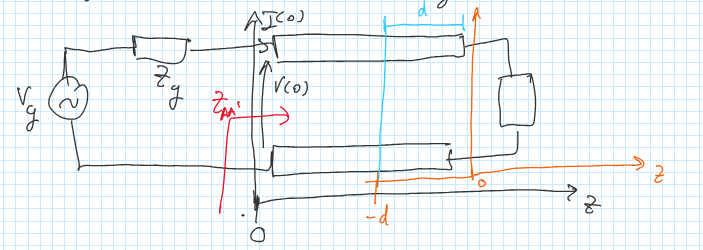
\includegraphics[width=0.75\linewidth]{Chapter_two/Chapt2img9.png}
        \end{figure} \\
        Fissata di nuovo l'origine alla sezione d'uscita, applichiamo semplicemente la formula per 
        ricavare il coefficiente di riflessione all'uscita:
        \begin{equation}
            \Gamma(0) = \Gamma_{OUT} = \frac{Z_{0}-Z_{C}}{Z_{C}+Z_{0}}
        \end{equation}
        in quanto $Z(0)=Z_{C}$. A questo punto possiamo calcolarlo in un punto generico della linea:
        \begin{equation}
            \Gamma(-d) = \Gamma(0)e^{-j 2 \beta d}
        \end{equation}
        Con la stessa formula potremmo ricavare $\Gamma_{AA'}$, il coefficiente di riflessione alla sezione 
        d'ingresso AA' e di conseguenza $Z_{AA'}$. Dunque si può partire sia da $\Gamma$ che da $Z$ a seconda 
        di come ci conviene!

    \subsection*{Carico puramente reattivo}
        Primo di tre casi particolari che studieremo. Per il carico puramente reattivo, $Z_{C}=jX_{c}$, dunque 
        non c'è flusso di potenza attiva.
        \begin{figure}[h!]
            \center  
            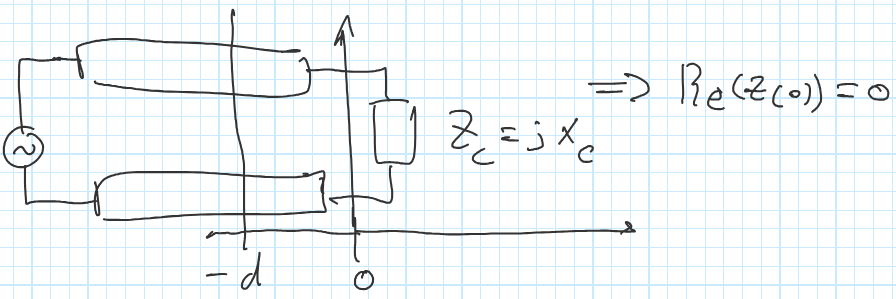
\includegraphics[width=0.5\linewidth]{Chapter_two/Chapt2img10.png}
        \end{figure} \\
        Calcoliamo l'impedenza in un punto a distanza $d$ rispetto alla sezione d'uscita:
        \begin{equation}
            Z(-d) = Z_{0} \frac{jX_{C}+jZ_{0}\tan(\beta d)}{Z_{0}+j^{2}X_{C}\tan(\beta d)} = jZ_{0} \frac{X_{C}+Z_{0}\tan(\beta d)}{Z_{0}-X\tan(\beta d)}
        \end{equation}
        Cioè per un carico puramente reattivo si ha trasporto puramente reattivo. Per quanto concerne il coefficiente 
        di riflessione:
        \begin{equation}
            \Gamma (0) = \frac{jX_{C}-Z_{0}}{jX_{C}+Z_{0}} \implies \Gamma(-d) \frac{jX_{C}-Z_{0}}{jX_{C}+Z_{0}}e^{-j2\beta d}
        \end{equation}
        \begin{equation}
            \implies |\Gamma (-d)| = \frac{|jX_{C}-Z_{0}|}{jX_{C}+Z_{0}} = 1
        \end{equation}
        Per un carico puramente riflessivo c'è riflessione totale.
    \subsection*{Carico in corto circuito}
        Facciamo riferimento al disegno per il carico puramente reattivo da ora in avanti.
        Per un corto circuito $Z_{C}=0$, dunque non c'è né potenza reattiva né potenza attiva propagata.
        Calcolando il trasporto d'impedenza lungo la linea:
        \begin{equation}
            Z(-d ) = Z_{0}\frac{0 +jZ_{0}\tan(\beta d)}{Z_{0}+0} = jZ_{0}\tan(\beta d)
        \end{equation}
        cioè viene trasportata in modulo la stessa impedenza, quella caratteristica della linea, che cambia fase 
        in funzione di $d$. Il coefficiente di riflessione è immediato:
        \begin{align}
            |\Gamma|=|\frac{0-Z_{0}}{0+Z_{0}}|=1 \\
            \angle \Gamma = \angle \frac{-Z_{0}}{Z_{0}} = \pi
        \end{align}
        Dunque il corto parte da $\Gamma(0)=e^{-\pi} = -1$ e varia sulla linea come $\Gamma(-d) = -e^{-j2\beta d}$
    \subsection*{Carico in circuito aperto}
        Per un circuito aperto conviene lavorare con le ammettenze, 
        che in questo caos è $Y_{C}=0$ al carico, pertanto:
        \begin{align}
            Y(-d) = j y_{0}\tan(\beta d) \\
            |\Gamma| = 1 \\
            \angle \Gamma = 1
        \end{align}
        Dunque il circuito aperto parte con $\Gamma(0)=1$ e varia sulla linea come $\Gamma(-d)=e^{-j2 \beta d}$
    \newpage 
    \section{Andamento dei parametri di linea}
    Continuiamo il discorso per le linee di trasmissione omogenee
    \begin{figure}[h!]
        \center  
        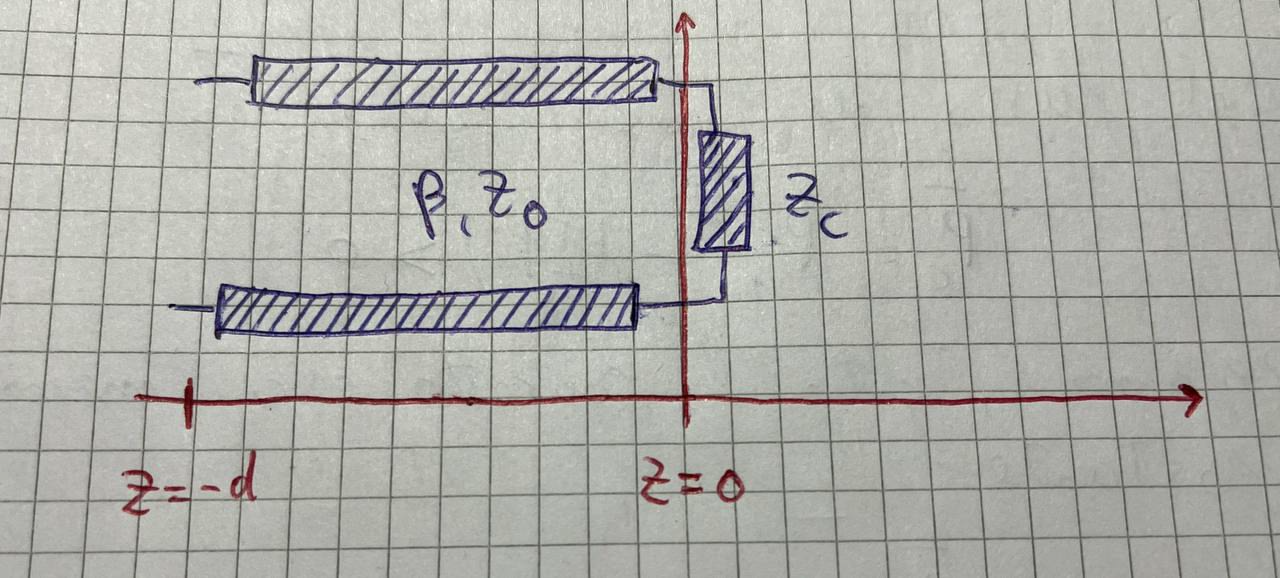
\includegraphics[width=0.6\linewidth]{Chapter_two/Chapt2img11.png}
    \end{figure}
    Consideriamo le quantità:
    \begin{equation}
        |\frac{V_{C}}{V^{+}}| = |1+\Gamma_{C}| \qquad |\frac{I_{C}}{I^{+}}| = |1-\Gamma_{C}|
    \end{equation}
    Allora per un corto ($Z_{C}=0$) poiché $\Gamma_{C}=-1$:
    \begin{equation}
        |\frac{V_{C}}{V^{+}}| = 0 \qquad |\frac{I_{C}}{I^{+}}|=2
    \end{equation}
    come ci aspettavamo, il modulo della tensione è nulla, cioè il minimo valore possibile sulla linea, 
    mentre ha il massimo valore di modulo di tensione sulle linea pari a $|V_{C}|=2|V^{+}|$. Per un aperto 
    ($Y_{C}=0$) c'è $\Gamma = 1$ e dunque:
    \begin{equation}
        |\frac{V_{C}}{V^{+}}|=2 \qquad |\frac{I_{C}}{I^{+}}|=0
    \end{equation}
    Per l'aperto si ha il modulo massimo della tensione pari a $2V^{+}$ e minimo valore del modulo di corrente. 
    \\ Consideriamo ora un carico generico $Z_{C}=R_{C}+jX_{C}$. In questo caso c'è il flusso di potenza 
    attiva $\overline{P}_{C}$:
    \begin{equation}
        \overline{P}_{C}=\overline{P}^{+}(1-|\Gamma_{C}|^{2}) > 0
    \end{equation}    
    Normalizziamo perché tanto il concetto vale a meno di una costante:
    \begin{equation}
        |\frac{\overline{P}}{P^{+}}| = 1-|\Gamma_{C}|^{2}
    \end{equation}
    Infatti si può dimostrare che per una linea con carico con parte reale maggiore di zero $\Gamma_{C}<1$.
    Se ci si mette nel piano complesso e si disegna il vettore $|1+\Gamma_{C}$, ci si rende conto che questo ha modulo 
    massimo quando $1$ e $\Gamma_{C}$ sono in fase, cioè quando $2\beta d + \phi_{c} = 2 n \pi$.
    \newpage
    \begin{figure}[h!]
        \center  
        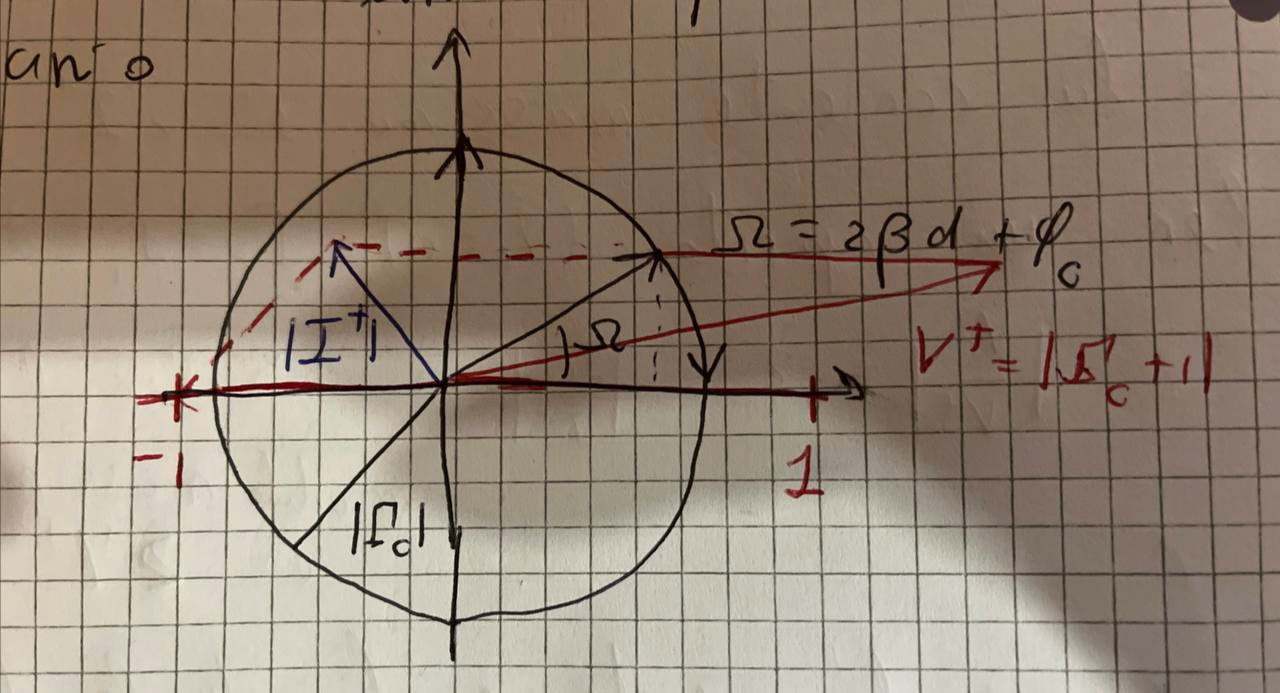
\includegraphics[width=0.5\linewidth]{Chapter_two/Chapt2img12.png}
    \end{figure} 
    Vogliamo trovare ora massimo e minimo per linee con impedenze di carico con parte reale stettamente maggiore di zero.
    Esplichiamo l'espressione:
    \begin{equation} 
        \Re(Z(d)) = Z_{0}\Re[\frac{1+\Gamma(d)}{1-\Gamma(d)}] = Z_{0}\Re[\frac{(1+\Gamma(d)(1-\Gamma(d)^{*}))}{-2\Re(\Gamma(d))+1+|\Gamma|^{2}}]
    \end{equation}
    \begin{equation}
        = Z_{0}\Re[\frac{2+2\Im(\Gamma(d)-|\Gamma|^{2})}{1+|\Gamma|^{2}-2\Re(\Gamma(d))}] = \frac{(1-|\Gamma|)(1+|\Gamma|)}{1+|\Gamma|^{2}-2\Re(\Gamma(d))} > 0
    \end{equation}
    Questo numero è minimo quando il numeratore è massimo, cioè quando la parte reale di $\Re(\Lambda(d))$ è pari all'opposto del suo modulo:
    \begin{equation}
        \textrm{Minimo denominatore} = 1+|\Gamma|^{2}-2\Re(\Gamma (d))
    \end{equation}
    Mentre il massimo è $1+|\Gamma ^{2}|+2\Re(\Gamma (d))$. Il minimo si ottiene per fase negativa mentre 
    il massimo per fare positiva. A fronte di ciò, il minimo valore della parte reale dell'impedenza sulla linea è:
    In entrambi i casi $\Gamma$ è totalmente reale e visto che il modulo è costante $\Re(\Gamma) = |\Gamma|$. Allora:
    \begin{equation}
        1+|\Gamma|^{2}-2\Re(\Gamma (d)) = (1-|\Gamma|)^{2} \qquad 1+|\Gamma|^{2}+2\Re(\Gamma (d)) =(1+|\Gamma|)^{2}
    \end{equation}
    \begin{equation}
         \implies \Re_{min}(Z(d)) = Z_{0} \frac{(1-|\Gamma|)(1+|\Gamma|)}{(1-\Gamma)^{2}}=Z_{0}\frac{1-|\Gamma|}{1+|\Gamma|} > 0
    \end{equation}
    \begin{equation}
        \implies \Re_{max}(Z(d))=Z_{0}\frac{1+|\Gamma|}{1-|\Gamma|}
    \end{equation}
    Si noti che sia per il massimo che per il minimo la parte immaginaria dell'impedenza è zero, perché $\Gamma$ è puramente reale.
    \section*{Carico puramente reattivo}
    Consideriamo ora una linea omogenea senza perdite e con carico $Z_{C}$. Analizziamo il caso per il quale $Z_{C}=jX_{C}$, ovvero c'è 
    un carico puramente reattivo. Facendo il trasporto d'impedenza a generica distanza $d$:
    \begin{equation}
        Z(d) = Z_{0} \frac{j(X_{C}+Z_{0}\tan(\beta d))}{Z_{0}-X_{C}\tan(\beta d)}
    \end{equation}
    puramente immaginaria, come ben sappiamo. La $Z(d)$ non è limitata in modulo. In particolare si ottiene 
    un corto per l'annullarsi del nominatore ed un aperto nel caso si annulli il denominatore:
    \begin{equation}
        \frac{Z_{0}}{X_{C}} = \tan(\beta d) \implies Z(d) = + \infty \qquad \frac{Z_{0}}{X_{C}}=-\tan(\beta) \implies Z(d) = 0
    \end{equation}
    Dimostriamo ora che sulla linea corti e aperti sono distanti di $\lambda/4$\footnote{Ricordiamo che $\lambda = 2\pi/\beta$}.\\
    \textbf{Proof}: \\
    Consideriamo una linea omogenea con carico $Z_{C}$ e due diverse distanze dal carico, $d'$ e $d$. Supponiamo che in $d'$ ci sia un corto 
    e dunque $Z(d')=0$, mentre in $d$ un aperto, per cui $Z(d)=+\infty$. Applichiamo il trasporto per un aperto:
    \begin{equation}
        Z(d)=jZ_{0}\tan(\beta d) \qquad \textrm{con } \beta = \frac{\pi}{2}+n \pi \ \ n \geq 0
    \end{equation}
    dove $n\geq 0$ perché $\beta d$ non può essere negativo per ovvi motivi fisici.\footnote{$d$ è una distanza, $\beta$ l'inverso di una lunghezza d'onda}
    Dunque il primo aperto si ha per $\beta = \frac{\pi}{2}$ e poiché $\beta = 2\pi/\lambda$:
    \begin{equation}
        \frac{2\pi}{\lambda}d = \frac{\pi}{2} \implies d = \frac{\lambda}{4}
    \end{equation}
    Allo stesso modo, per il corto ragioniamo con le ammettenze e consideriamo il primo aperto:
    \begin{equation}
        Y(d) = j y_{0}\tan(\beta d) \qquad \textrm{con } \beta d = \frac{\pi}{2}+n \pi
    \end{equation}
    \begin{equation}
        \implies \frac{2 \pi}{\lambda} d = \frac{\pi}{2} \implies d = \frac{\lambda}{4}
    \end{equation}
    Entrambe le espressioni sono periodiche di $\lambda/2$, dunque è facile intuire che ogni $\lambda/4$ si alterna corto, aperto, corto ... \\ \\
    La stessa cosa si può vedere nel piano complesso:
    \begin{figure}[h!]
        \center  
        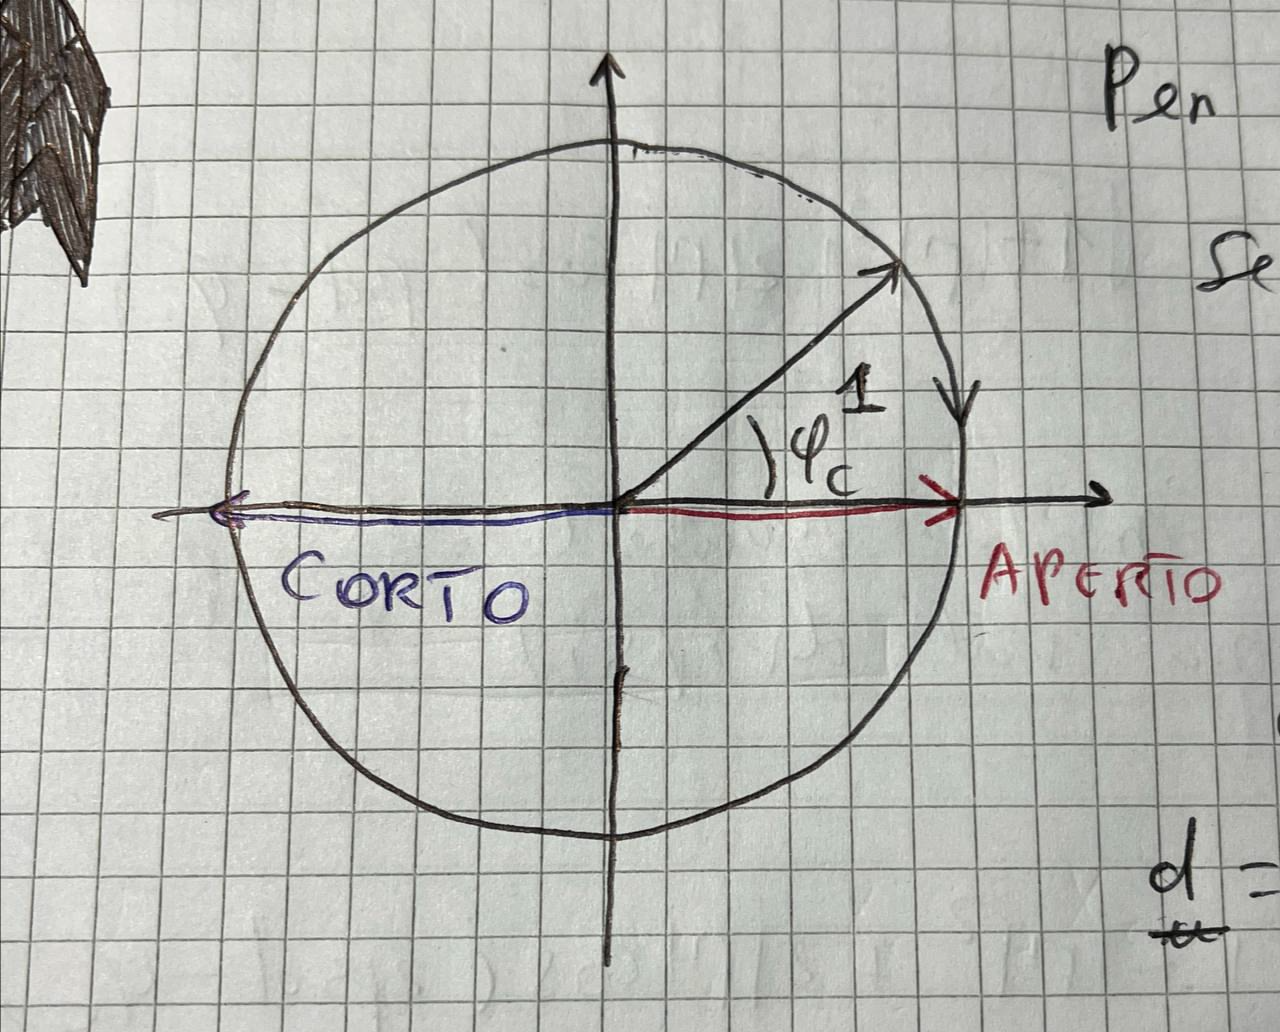
\includegraphics[width=0.5\linewidth]{Chapter_two/Chapt2img13.png}
    \end{figure}
    \\ Partendo con fase generica $\varphi_{c}$, si ha l'aperto quando la fase è nulla, cioè per:
    \begin{equation}
        \label{eqn:max_tensione}
        2 \beta d + \varphi_{c} = 2n \pi
    \end{equation}
    Similmente, si ottiene il corto quando $\Gamma=-1$, cio per fase è $\pi$:
    \begin{equation}
        \label{eqn:max_corrente}
        2\beta d + \varphi_{c}=2 n \pi + \pi
    \end{equation}
    \\ \\ 
    Vediamo come variano i \textbf{moduli} di tensione e corrente lungo la linea. Esprimiamo l'andamneto come rapporto fra il modulo
    della tensione e il parametro $V^{+}$, perché l'andamento  (la "forma" della funzione) è indipendente da quest'ultimo:
    \begin{align}
        V(d) = V^{+}(1+\Gamma (d)) \implies \frac{|V(d)|}{|V^{+}|} = |1+\Gamma (d)| \\
        \implies |1+\Gamma_{R}(d)+j \Gamma_{Im}(d)| = \sqrt{(1+\Gamma_{R})^{2}+\Gamma_{Im}^{2}(d)} \\
        = \sqrt{1 + 2 \Gamma_{R}(d)+|\Gamma|^{2}}
    \end{align}
    L'ultimo passaggio è giustificato dal fatto che $\Gamma_{R}^{2}+\Gamma_{Im} ^{2} = |\Gamma|^{2}$. Tenendo conto che:
    \begin{equation}
        \Re(\Gamma (d)) = \Re(|\Gamma|e^{j \varphi_{c}}e^{-j 2 \beta d}) = |\Gamma|\cos(2\beta d - \varphi_{c})
    \end{equation}
    si ottiene, in definitiva:
    \begin{equation}
        \frac{|V(d)|}{|V^{+}|} = \sqrt{1 + |\Gamma|^{2}+2|\Gamma|\cos(2 \beta d- \varphi_{c})}
    \end{equation}
    È una funzione sinuosidale di periodo $\lambda/2$ che ha massimi per $2\beta d - \varphi_{c} = 2n \pi$, quando il coseno è massimo. 
    \begin{figure}[h!]
        \center  
        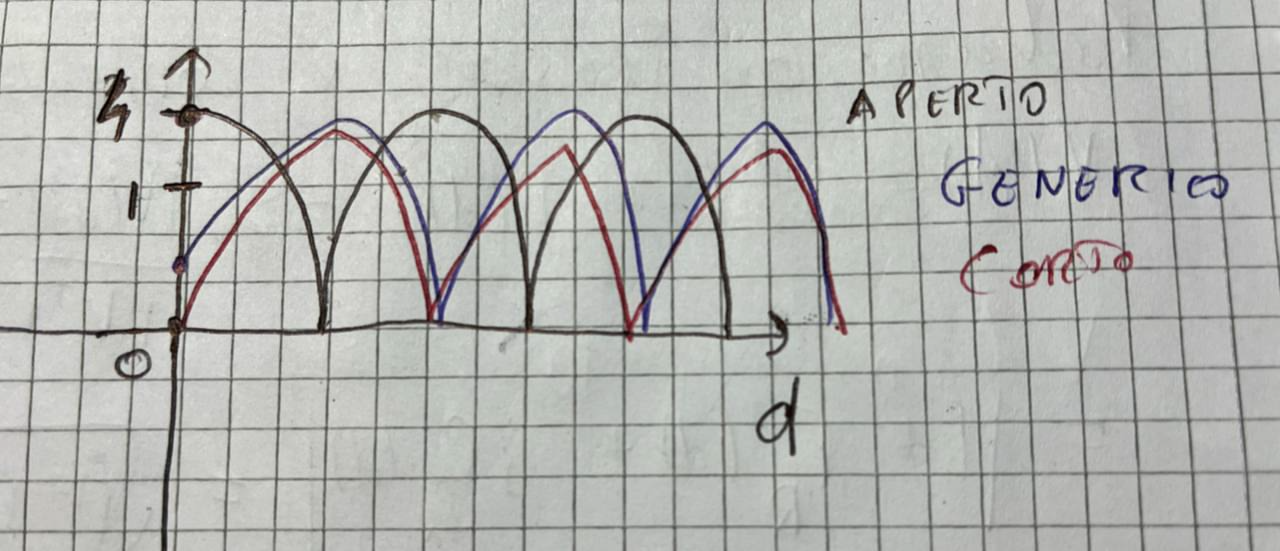
\includegraphics[width=0.65\linewidth]{Chapter_two/Chapt2img14.png}
    \end{figure}
    \\
    Che abbia periodo $\lambda/2$ è immediato, perché il coseno ha pulsazione $2 \beta d$.
    Per la corrente l'espressione che si ottiene è la stessa a meno di un segno, facendo gli stessi identici 
    passaggi di sopra:
    \begin{equation}
        \frac{|I(d)|}{|I^{+}|} = \sqrt{1+|\Gamma|^{2}-2|\Gamma|\cos(2 \beta d - \varphi_{c})}
    \end{equation}
    Il grafico della corrente è, senza troppe sorprese, traslato di $\pi/2$ rispetto a quello della tensione. \\
    Gli stessi risultati si potevano ottenere dall'espressione dei coefficienti di riflessione:
    \begin{equation}
        \label{eqn:pippo}
        \frac{|V(d)|}{|V^{+}|}=|1+\Gamma(d)|
    \end{equation}
    ha un massimo per $\Gamma(d)$, cioè per $2\beta d-\varphi_{c} = 2n \pi$. Allo stesso modo:
    \begin{equation}
        \label{eqn:pluto}
        \frac{|V(d)|}{|V^{+}|}=|1-\Gamma(d)|
    \end{equation}
    ha massimo per $\Gamma(d) = -1$, cioè per $2\beta d-\varphi_{c} = \pi + 2n \pi$. 
    E questa cosa ha perfettamente senso ! Infatti (\ref{eqn:pippo}) è la condizione per avere un aperto, 
    per il quale si ha il massimo di tensione $|V(d)|=2|V^{+}|$, mentre (\ref{eqn:pluto}) è la condizione per il chiuso,
    per il quale c'è il massimo di corrente $|I(d)|=2|I^{+}|$. \\ \\
    Facciamo una precisazione su una cosa leggermente tricky. Consideriamo una linea di trasmissione lunga 
    $d < \lambda/4$ ed ipotizziamo che abbia un corto come carico. Il massimo di tensione dovrebbe stare a $\lambda/4$ dal corto,
    ma la linea è più corta. Allora il massimo è all'inizio della linea, perché la tensione è una funzione continua in $d$ che ha un 
    minimo in corrispondenza del corto, dunque il massimo c'è sempre, perché partendo dal minimo cresce a destra e a sinistra per $\lambda/4$. 
    
    \section*{Carico generico}
        In questo caso, la parte reale dell'impedenza di carico è maggiore di zero. Abbiamo già visto che 
        per impedenze con parti reali non nulle il coefficiente di riflessione è, in modulo, minore dell'unità. 
        L'espressione per i rapporti di moduli per tensione e corrente è analoga a prima:
        \begin{equation}
            \frac{|V(d)|}{|V^{+}|} = \sqrt{1+|\Gamma|^{2}+2|\Gamma|\cos(2\beta d - \varphi_{c})}
        \end{equation}
        Quella per la corrente varia di un segno. È facile vedere che entrambe le funzioni\footnote{Quando c'è il massimo per la tensione (corrente) $1+|\Gamma|^{2}\pm2|\Gamma| = (1 \pm |\Gamma|)^{2}$} variano nell'intervallo:
        \begin{equation}
            [1-|\Gamma|, 1+|\Gamma|]
        \end{equation}
        e avranno i massimi, come prima, in corrispondenza dei valori per i quali il coseno è massimo in modulo, che sono gli stessi
        di prima. \\
        \begin{center}
        \begin{tabular}{c|c|c} 
            $2 \beta d - \varphi_{c}=2\pi n$ & $\max V$ & $\min I$ \\
            $2\beta d - \varphi_{c}=2 \pi n + \pi$ & $\min V$ & $\max I$
        \end{tabular}
        \end{center} 
        In questo caso\footnote{Cioè in corrispondenza di massimi e minimi}, quando il coefficiente di riflessione è puramente reale, abbiamo carico puramente 
        resistivo:
        \begin{equation}
            Z(d) = Z_{0} \frac{1-|\Gamma|^{2}+j2\Gamma_{I}(d)}{1+|\Gamma|^{2}-2 \Gamma_{R}(d)} = Z_{0}\frac{1-|\Gamma|^{2}}{1+|\Gamma|^{2}-2|\Gamma|}
        \end{equation}
        \begin{equation}
            = \frac{1+|\Gamma|}{1-|\Gamma|}Z_{0} = R_{max}
        \end{equation}
        che è il massimo valore di resistenza trasportabile. Viceversa, per $\Gamma$ reale negativo c'è il minimo valore di resistenza trasportabile:
        \begin{equation}
            R_{min}=\frac{1-|\Gamma|}{1+|\Gamma|}
        \end{equation}
        In sintesi la parte reale dell'impedenza è compresa fra i valori:
        \begin{equation}
            \frac{1-|\Gamma|}{1+|\Gamma|} \leq \Re(Z(d)) \leq \frac{1+|\Gamma|}{1-|\Gamma|} 
        \end{equation}
        che sono entrambi valori positivi, come ci aspettavamo. Se non fosse così, infatti, ci sarebbe almeno un punto con potenza attiva propagata nulla e di
        conseguenza su tutta la linea non ci sarebbe propagazione di potenza attiva.
        
    \section{Linee con discontinuità ed adattamento}
    \subsection*{Linee con discontinuità}
    Consideriamo ora il caso di linee che presentano discontinuità, come nel disegno a seguire:
    \begin{figure}[h!]
        \center  
        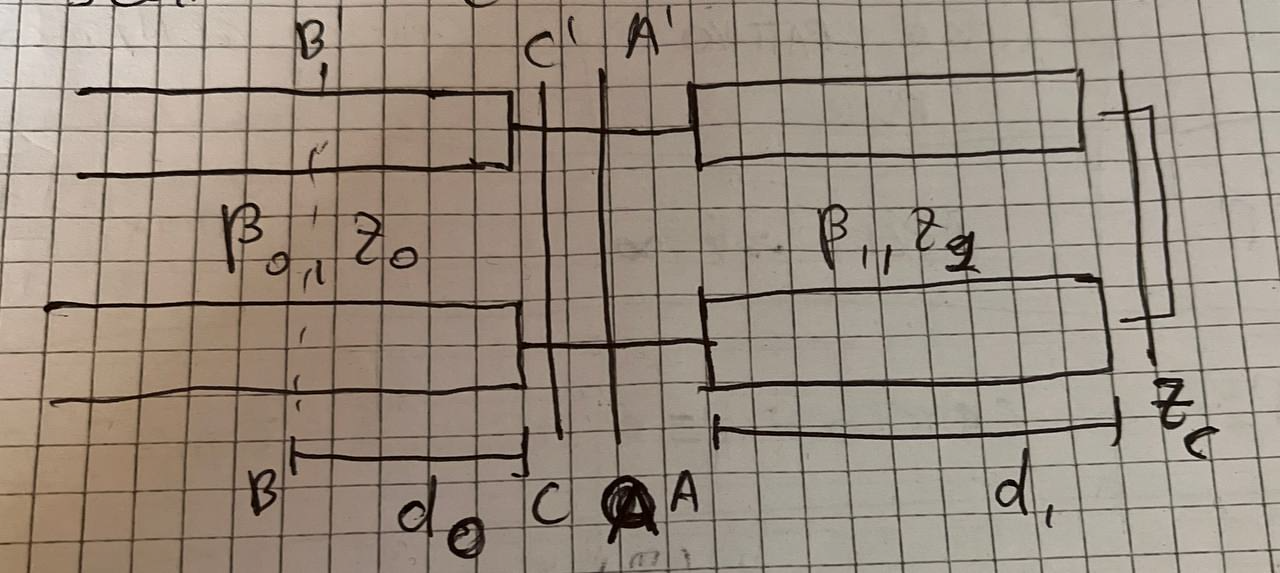
\includegraphics[width=0.6\linewidth]{Chapter_two/Chapt2img15.png}
    \end{figure}
    Vogliamo calcolare il trasporto d'impedenza nel punto a distanza $d_{0}$ dall'inizio della prima linea, tenendo conto che la seconda 
    linea è lunga $d_{1}$. La prima e la seconda linea sono caratterizzate rispettivamente da $(\beta_{0}, Z_{0})$ e $(\beta_{1}, Z_{1})$.
    Per risolverlo, si calcola prima l'impedenza vista dalla linea alla sezione $AA'$:
    \begin{equation}
        Z_{AA'} = Z_{1} \frac{Z_{C}+jZ_{1}\tan(\beta d_{1})}{Z_{1}+jZ_{C}\tan(\beta d_{1})} = j Z_{1}\tan(\beta d_{1})
    \end{equation}
    perché siamo nel caso semplice dove c'è un corto come carico. A questo punto bisogna semplicemente trasportare:
    \begin{equation}
        Z_{BB'} = Z_{0} \frac{Z_{AA'}+jZ_{0}\tan(\beta d_{0})}{Z_{0}+jZ_{AA'}\tan(\beta d_{0})}
    \end{equation}
    Qual è l'ipotesi sotto la quale regge ciò che abbiamo appena fatto? Che l'impedenza sia continua lungo la discontinuità 
    e che quindi $Z_{AA'}=Z_{CC'}$. In altri termini, abbiamo supposto che l'impedenza alla fine della linea coincida con quella all'inizio 
    di quella successiva. L'ipotesi di continuità dell'impedenza è in realtà conseguenza dell'ipotesi più generale che tensione e corrente 
    siano continue su tutta la linea e, di conseguenza, lo sono anche le impedenze e la potenza complessa.
    \begin{equation}
        \begin{cases}
            V_{AA'}=V_{BB'} \\
            I_{AA'} = I_{BB'}
        \end{cases} \implies 
        \begin{cases}
            Z_{AA'} = Z_{BB'} \\
            \hat{P}_{AA'} = \hat{P}_{BB'}
        \end{cases}
    \end{equation}
    Ciò che abbiamo detto non vale, però per il coefficiente di riflessione.  \\
    \textbf{Proof}: \\
    Per dimostrarlo supponiamo, riferendoci al disegno 
    di prima, di avere una resistenza $R_{C}<Z_{1}$ come carico al posto del corto. Supponiamo inoltre che $d=\lambda_{1} /4$. Calcolando $Z_{AA'}$ si ricava:
    \begin{equation}
        Z_{AA'} = Z_{1}\frac{R_{C}+jZ_{1}\tan(\beta \frac{\lambda_{1}}{4})}{Z_{1}+jR_{C}\tan(\beta \frac{\lambda_{1}}{4})}
    \end{equation}
    Poiché:
    \begin{equation}
        \frac{\lambda}{4}\beta = \frac{2\pi}{\lambda} \cdot \frac{\lambda}{4}=\frac{\pi}{2}
    \end{equation}
    l'espressione di sopra può essere approssimata al rapporto delle due tangenti, che divergono per $\pi/2$:
    \begin{equation}
        Z_{AA'} \simeq \frac{Z_{1} ^{2}}{R_{C}}
    \end{equation}
    che è una quantità sicuramente maggiore di $Z_{1}$, sotto l'ipotesi $R_{C}<Z_{1}$.
    A questo punto, otteniamo la seguente linea equivalente:
    \begin{figure}[h!]
        \center  
        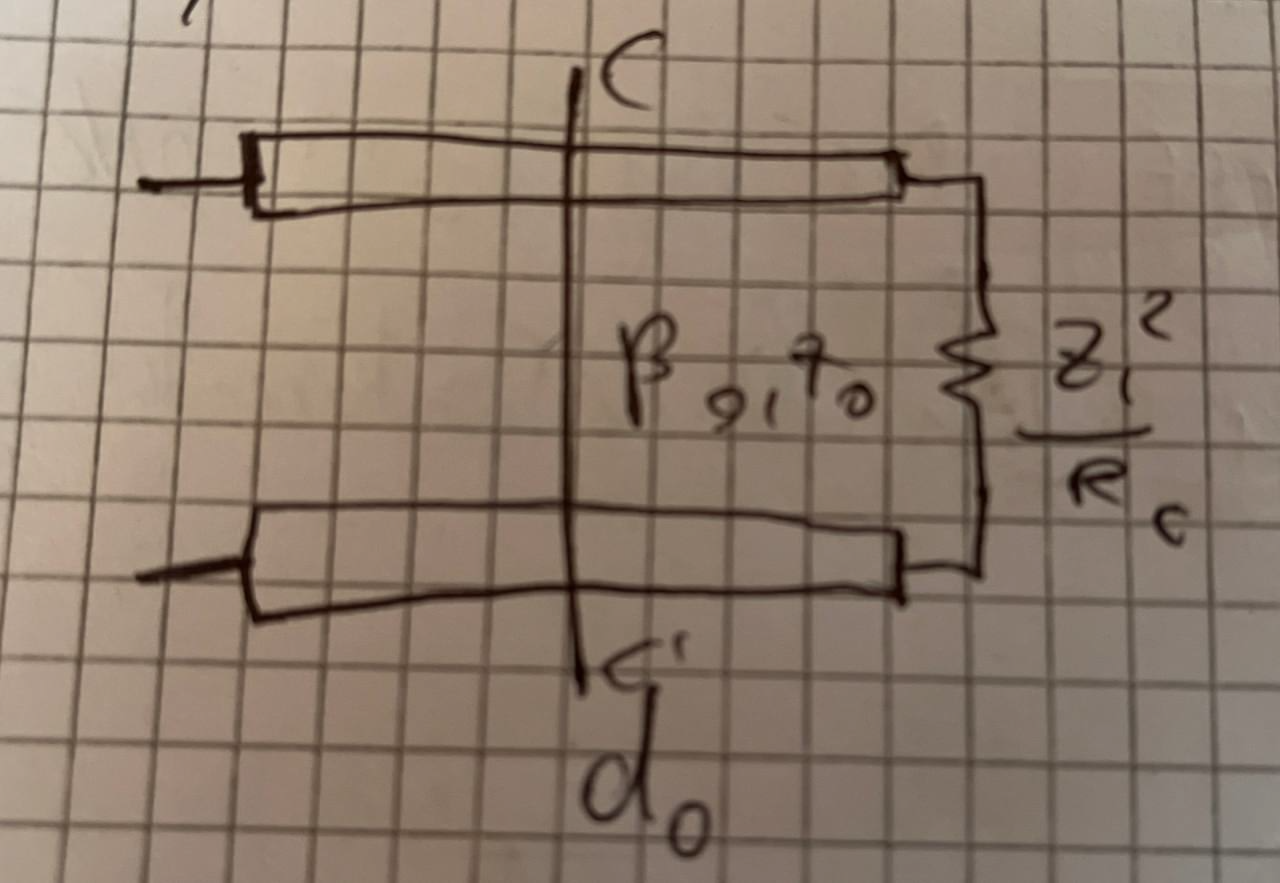
\includegraphics[width=0.6\linewidth]{Chapter_two/Chapt2img16.png}
    \end{figure}
    Calcoliamo il coefficiente di riflessione in $Z_{BB'}$\footnote{cioè alla fine della seconda linea, ho dimenticato di disegnarlo}:
        \begin{equation}
            \Gamma_{CC'} = \frac{R_{C}-Z_{1}}{R_{C}+Z_{1}} < 0
        \end{equation}
    Tenendo conto che il coefficiente alla sezione AA' (inizio della seconda linea) è:
    \begin{equation}
        \Gamma_{AA'} = \Gamma_{BB'}e^{-j 2 \beta \lambda/4} = \Gamma_{BB'}e^{-j \pi} = -\Gamma_{BB'} \neq \Gamma_{CC'}
    \end{equation}
    in quanto:
    \begin{equation}
        \Gamma_{CC'} = \frac{Z_{1} ^{2} /R_{C} -Z_{0}}{Z_{1} ^{2} +Z_{0}} \neq - \Gamma_{BB'}
    \end{equation}
    \\ \\
    Un ulteriore caso di interesse applicativo è quello per il quale si conosce il coefficiente di riflessione di una delle due linee, per esempio la seconda, ma 
    non l'impedenza di carico. Quello che si fa è semplicemente calcolare l'impedenza di carico tramite il coefficiente di riflessione è poi applicare il trasporto.
    Se poi si conosce quello della prima, si può direttamente calcolare con la ben nota relazione:
    \begin{equation}
        Z_{CC'} = Z_{1}\frac{1+\Lambda_{CC'}}{1-\Lambda_{CC'}}
    \end{equation}
    Fisicamente, il fatto che il coefficiente di riflessione non si conservi ma il resto delle grandezze si, significa che la proporzione di onda 
    regressiva ed onda progressiva varia nel tempo, ma la loro somma resta costante:
    \begin{equation}
        V^{+}_{AA'}+V^{-} _{AA'} = V^{+}_{BB'}+V^{-} _{BB'}
    \end{equation}
    \subsection*{Adattamento}
        Consideriamo una situazione del genere:
        \begin{figure}[h!]
            \center  
            \includegraphics[width=0.65\linewidth]{Chapter_two/chapt2img17}
        \end{figure}
        Il nostro interesse è il trasferimento massimo di potenza attiva al carico. Sappiamo che 
        la massima potenza attiva che il generatore può trasferire al carico è pari a:
        \begin{equation}
            P_{max} = \frac{1}{8} \frac{|V_{g}| ^{2}}{R_{g}}
        \end{equation}
        In pratica, vogliamo annullare il coefficiente di riflessione alla sezione d'ingresso.
        Sia $Z_{BB'}$ l'impedenza trasportata dal carico alla sezione d'ingresso. Affinché il coefficiente di riflessione 
        sia nullo deve risultare:
        \begin{equation}
            \Lambda_{IN} = \frac{Z_{BB'}-Z_{g}}{Z_{BB'}+Z_{g}} = 0 \implies Z_{g} = Z_{BB'}
        \end{equation}
        Per fare in modo che l'impedenza trasportata sia uguale a quella del generatore, bisogna inserire una
        \textbf{rete di adattamento} tra il generatore ed la linea. Si può fare la stessa cosa tra linea e carico e in quel caso si 
        parla di adattamento \textit{al carico}, invece che \textit{al generatore}. La linea non deve introdurre perdite e 
        non linearità, quindi deve essere fatta da soli \textbf{elementi lineari reattivi od al massimo linee senza perdite }.
    \subsubsection{Adattatore a $\lambda/4$}
        L'adattatore a $\lambda/4$ è il primo dei due adattatori che vediamo in questa sezione. Come suggerisce il nome,
        è costituito da una linea lunga $\lambda/4$ interposta fra la linea e il carico:
        \begin{figure}[h!]
            \center  
            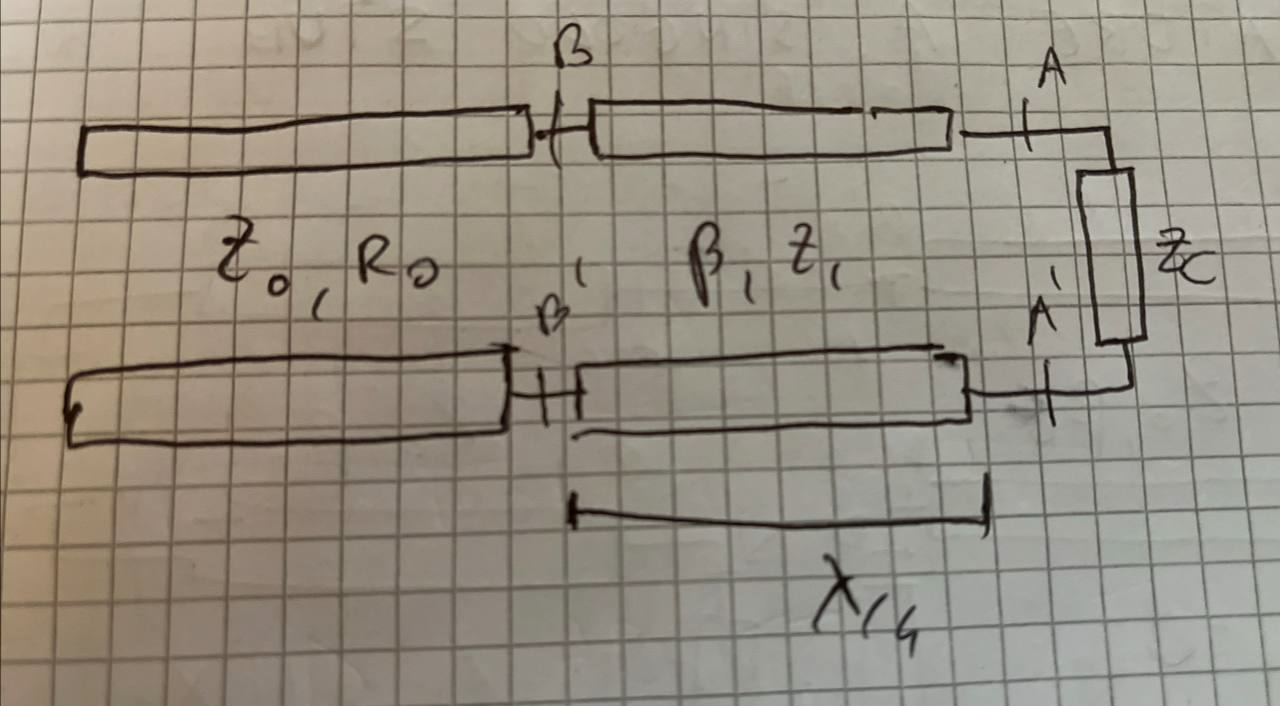
\includegraphics[width=0.6\linewidth]{Chapter_two/Chapt2img18.png}
        \end{figure}
        Ovviamente non basta che l'adattatore sia lungo $\lambda/4$, ma deve soddisfare ulteriori proprietà.
        Sia la linea da adattare che l'adattatore devono avere, infatti, impedenza caratteristica reale. Nel nostro caso, $Z_{1}$ e $Z_{0}$. Inoltre 
        l'adattatore deve avere $\beta_{1}$ reale. La terza condizione è che anche il carico sia puramente reale.
        \\ Fatte queste premesse, possiamo caclolare il trasporto all'inizio dell'adattatore:
        \begin{equation}
            Z_{BB'} = Z_{0} = Z_{1} \cdot \frac{Z_{C}+jZ_{1}\tan(\beta \lambda /4)}{Z_{1}+jZ_{C}\tan(\beta \lambda /4)} \simeq \frac{Z_{1} ^{2}}{Z_{C}} = Z_{0}
        \end{equation}
        Da cui si ottiene:
        \begin{equation}
            Z_{1} \simeq \sqrt{Z_{0}Z_{C}}
        \end{equation}
        che va sotto il nome di \textbf{formula di adattamento}.
    \newpage
        \subsubsection*{Adattatore a singolo stub}
        \begin{figure}[h!]
            \center  
            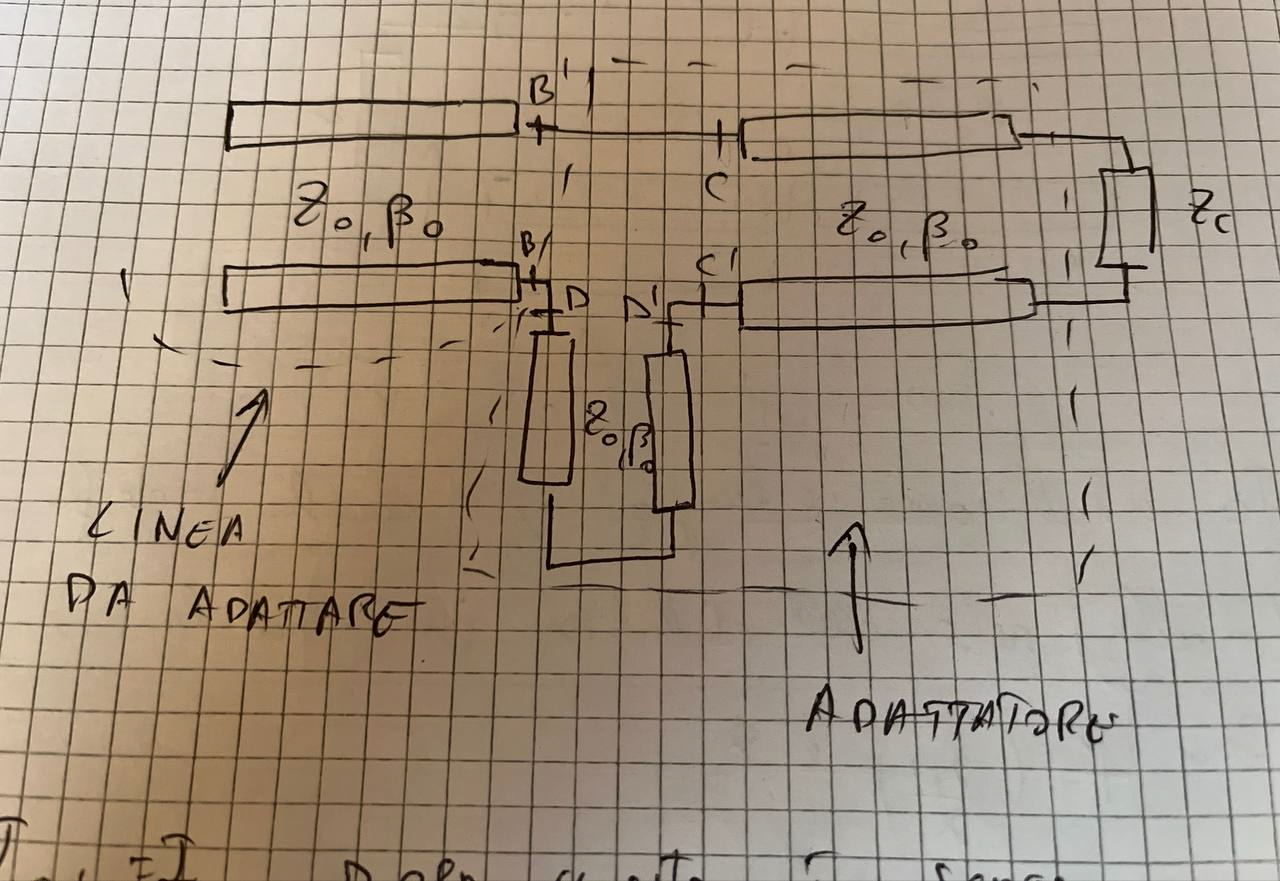
\includegraphics[width=0.5\linewidth]{Chapter_two/Chapt2img19.png}
        \end{figure}
        In questa sezione presentiamo solo la forma dell'adattatore a singolo stub, che poi verrà trattato
        ampiamente negli esercizi. Quello in figura è un adattatore a singolo stub \textbf{in serie}, perché la corrente che scorre all'interno
        dello stub (la linea in verticale sotto) è la stessa che scorre all'interno della linea di adattamento collegata subito prima del carico.
        La configurazione in parallelo è la stessa con l'unica eccezione che lo stub e la linea da adattare sono connessi, per l'appunto, in parallelo.
        \\ \\
        Ipotizziamo che il carico si $Z_{C}=R_{C}+jX_{C}$, la lunghezza dello stub $y$ (incognita) e quella della linea di adattamento $x$, anch'essa incognita.
        Ci viene richiesto, di solito, di ricavare i valori di $x$ ed $y$ per i quali la rete è adattata.
        \begin{figure}[h!]
            \center  
            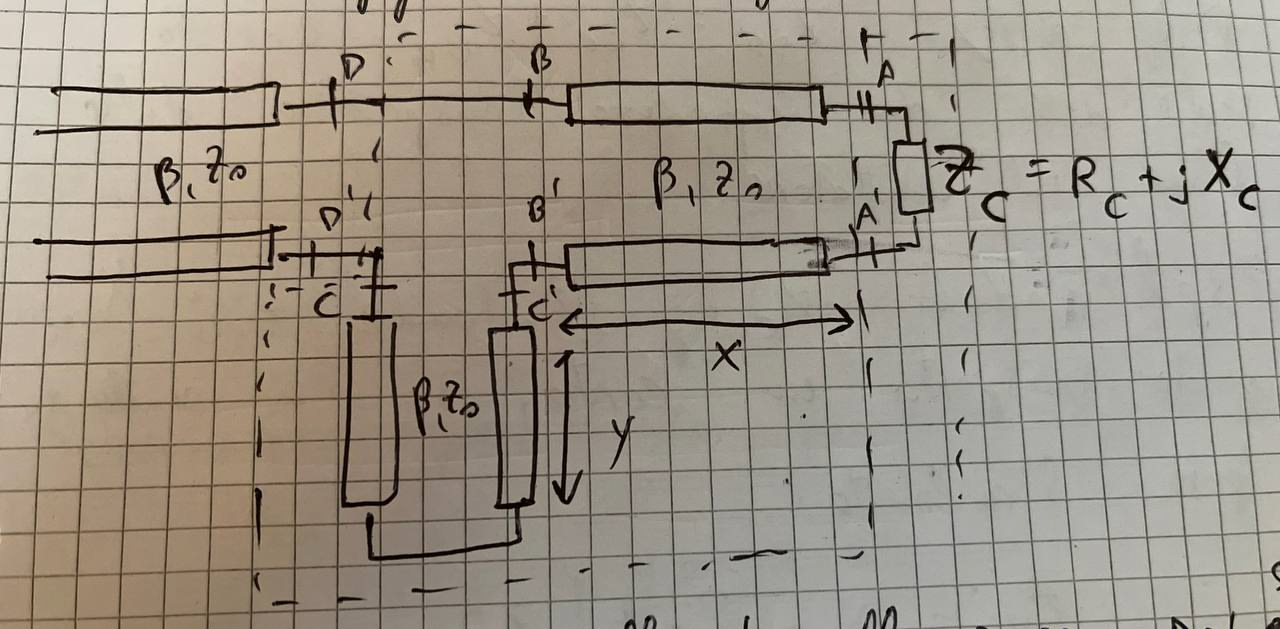
\includegraphics[width=0.6\linewidth]{Chapter_two/Chapt2img20.png}
        \end{figure}
        Le condizion di adattamento sono, nel nostro caso:
        \begin{equation}
            Z_{DD'} = Z_{0} ^{*}
        \end{equation}
        Supponendo che $Z_{0}$ sia reale, bisogna verificare:
        \begin{equation}
            R_{DD'} = Z_{0} \\
            X_{DD'} = 0
        \end{equation}
        È sempre possibile trovare valori di $x$ ed $y$ reali non negativi\footnote{Sono lunghezze !} tali da soddisfare le condizioni 
        di adattamento? La rispota è affermativa.
        \\ \textbf{Proof}: 
        \\ Si vede dal disegno che :
        \begin{equation}
            Z_{DD'} = Z_{CC'}+Z_{BB'}
        \end{equation}
        perché siamo in configurazione serie. Lo stesso discorso vale per le ammettenze per la configurazione parallelo.
        Esplicandole e tenendo conto che lo stub trasporta un corto:
        \begin{align*}
            Z_{CC'} = jZ_{0}\tan(\beta y) = jX_{CC'}(y) \\
            Z_{BB'} = Z_{0} \cdot \frac{Z_{C}+jZ_{0}\tan(\beta x)}{Z_{0}+jZ_{C}\tan(\beta x)} = R_{BB'}(x)+jX_{BB'}(x)
        \end{align*}
        A questo punto bisogna verificare:
        \begin{equation}
            \begin{cases}
                R_{BB}(x)=Z_{0} \\
                X_{CC'}(y)+X_{BB'}(x) = 0
            \end{cases}
        \end{equation}
        La prima equazione ammette sempre soluzione? Tenendo conto che:
        \begin{equation}
            Z_{0} \frac{1-|\Gamma|}{1+|\Gamma|} \leq R_{BB}(x) \leq Z_{0}\frac{1+|\Gamma|}{1-|\Gamma|}
        \end{equation}
        poiché $Z_{0}$ è compreso nell'intervallo di valori per cui varia $R_{BB}(x)$ e poiché l'impedenza è continua sulla linea,
        allora è sicuramente verificata per qualche valore di $x$. In tal modo $X_{BB'}(x) \in \mathbb{R}$ è anch'essa univocamente determinata.
        A questo punto bisogna verificare che esista qualche valore di $y$ per cui:
        \begin{equation}
            X_{CC'}(y)=-X_{BB'}(x) \implies Z_{0}\tan(\beta y) = -X_{BB'}(x)
        \end{equation} 
        La relazione è verificata perché $-X_{BB'}(x)$ è un numero reale e la tangente assume tutti i valori fra $-\infty$ e $+\infty$, dunque $y$ esiste.
    \section*{ROS e Carta di Smith}
        Il ROS (\textit{Rapporto di Onda Stazionaria}), per una linea senza perdite chiusa su di un carico, ha la seguente espressione operativa:
        \begin{equation}
            \textrm{ROS } = \frac{1+|\Gamma|}{1-|\Gamma|} \in [1, + \infty)
        \end{equation}
        che discende direttamente dalla definizione:
        \begin{equation}
            \textrm{ROS } \triangleq  \frac{|V(z)|_{max}}{|V(z)|_{min}} = \frac{|V^{+}|\max(|1+\Gamma|)}{V^{+}\min(|1+\Gamma|)} = \frac{1+|\Gamma|}{1-|\Gamma|} 
        \end{equation}
        Il ROS ci da un'informazione parziale sul coefficiente di riflessione, dandoci il modulo. Per ricavare la fase basta mettersi in corrispondenza di un massimo o di un minimo
        di corrente, dove la fase è nulla, ruotando nel piano complesso fino ad arrivare all'inizio del carico. L'angolo di rotazione necessario per arrivare all'inizio sarà la fase del ROS.
        \\ \\ 
        Un'altro strumento è la \textbf{carta di Smith}. Sia $\Gamma = \xi +j \eta$ il coefficiente di riflessione, che sappiamo essere un numero complesso.
        Vogliamo tracciare una coppia di curve parametriche di $\xi$ ed $\eta$, comprese nella circonferenza unitaria.\footnote{perché il modulo di $\Gamma$ è al massimo uno.} \\
        Per fare ciò, sia $Z=R+jX$ una certa impedenza da adattare. Possiamo scrivere:
        \begin{equation}
            Z=Z_{0}\frac{1+\Gamma}{1-\Gamma} \implies \frac{Z}{Z_{0}} =\frac{1+\Gamma}{1-\Gamma}
        \end{equation}
        ottenendo una carta di Smith universale indipendente dall'impedenza da adattare. Esprimiamo $\Gamma$:
        \begin{equation}
            \frac{Z}{Z_{0}}=\frac{1+\xi+j\eta}{1-\xi-j\eta} = \frac{(1+\xi+j\eta)(1-\xi-j\eta)}{1+\xi ^{2}+\eta ^{2}-2\xi} = \frac{1+2j\eta - \xi ^{2} -\eta ^{2}}{1+\xi ^{2} + \eta ^{2}- 2 \xi}
        \end{equation}
        Otteniamo due funzioni, una per la parte reale  $r$ ed una per quella immaginaria $x$:
        \begin{equation}
            \begin{cases}
                \displaystyle r = \frac{1-\xi ^{2}-\eta ^{2}}{1+\xi ^{2}+\eta ^{2}-2\xi} \in [1, +\infty) \\
                \displaystyle x = \frac{2 \eta}{1+\xi ^{2}+\eta ^{2}-2\xi} \in (-\infty, + \infty)
            \end{cases}
        \end{equation}
        le quali non sono altro che le curve parametriche che stavamo cercando. Supponiamo ora che $r$ sia un valore fissato. Possiamo scrivere:
        \begin{equation}
            1-\xi ^{2} - \eta ^{2}= r (1+\xi^{2}+\eta^{2}-2\xi) \implies \xi^{2}(r+1)+\eta^{2}(r+1)-2r \xi = 1-r
        \end{equation}
        Dividiamo per $(1+r)$ e  facciamo comparire il quadrato di binomio a primo membro aggiungendo e sottraendo
        $(\frac{r}{1+r})^{2}$:
        \begin{equation}
            \xi^{2}+\eta ^{2}-\frac{2r}{r+1}\xi + (\frac{r}{r+1} )^{2}- (\frac{r}{r+1} )^{2} = \frac{1-r}{1+r}
        \end{equation} 
        \begin{equation}
            \implies (\xi-\frac{r}{r+1}) ^{2}+\eta ^{2} = \frac{1-r^{2}+r^{2}}{(1+r)^{2}} = (\frac{1}{1+r})^{2}
        \end{equation}
        Dunque la funzione parte reale $r$ è una circonferenza parametrica con centro
         $C_{r} = \displaystyle (\frac{r}{r+1},0)$ e raggio $\displaystyle \frac{1}{1+r} = \rho_{r}$.
         Se per esempio $r=1$, avremo $\rho = 1$ e centro in $(\frac{1}{2}, 0)$. Visto che $r$ varia da $0$ a $+\infty$,
         il centro si muove sul semiasse positivo di $\varepsilon$, con raggio che si annulla all'infinito. \newpage
         Per la parte immaginaria il procedimento è analogo:
         \begin{equation}
            x = \frac{2\eta}{1+\xi ^{2}+\eta ^{2}-2\xi}
         \end{equation}
        Come prima, supponendo che $x \neq 0$, moltiplichiamo ambo membri per il denominatore del membro a sinistra, riordiniamo, dividiamo per $x$ e facciamo 
        comparire il quadrato di binomio, ottenendo un'altro set di circonferenze parametriche:
        \begin{equation}
            (\xi -1) ^{2}+(\eta-\frac{1}{x})^{2}=\frac{1}{|x|^{2}}
        \end{equation}
        Le circonferenze parametriche della parte immaginaria hanno centro $C_{x} = \displaystyle (1, \frac{1}{x})$ 
        e raggio $\rho_{x} = \displaystyle \frac{1}{|x|}$. I centri si muovono lungo la retta $\xi=1$.
        In definitiva otteniamo:
        \begin{figure}[h!]
            \center  
            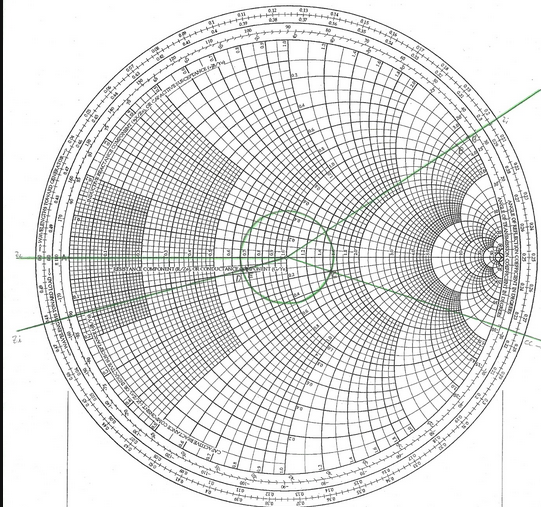
\includegraphics[width=0.6\linewidth]{Chapter_two/Chapt2img23.png}
        \end{figure}\\
        La carta di Smith offre un metodo grafico per ricavare i valori d'impedenza necessaria per adattare alla linea. Una volta
        ricavati $r$ ed $x$ tramite metodo grafico, conoscendo il rapporto $Z$ e $Z_{0}$ (pari a uno, per l'adattamento), posso calcolare $Z$ semplicemente
        moltiplicando $r$ ed $x$ per $Z_{0}$:
        \begin{equation}
            r+jx = \frac{R}{Z_{0}}+j\frac{X}{z_{0}}
        \end{equation}
        La stessa carta di Smith può essere utilizzata anche per le ammettenze, tenendo a mente che:
        \begin{equation}
            \frac{y}{Y_{0}} = \frac{1-\Gamma}{1+\Gamma} = \frac{1+\gamma}{1-\gamma}
        \end{equation}
        avendo posto $\gamma = -\Gamma$.
        Si possono allora ricavare $g$ e $b$ (conduttanza e suscettanza normalizzate) sapendo $y=-r$ e $b = -x$, 
        perché $\gamma = g+jb = -\Gamma = -r-jx$. \newpage 
        La carta di Smith non si limita a trovare i valori di adattamento, ma può essere utilizzata, per esempio, per ricavare 
        i valori minimi degli stub di adattamento per le linee. Consideriamo la seguente situazione
        \begin{figure}[h!]
            \center  
            \includegraphics[width=0.65\linewidth]{Chapter_two/chapt2img24}
        \end{figure}
        Conosco il carico $Z_{C}$, per cui conosco il coefficiente di riflessione corrispondente $\Gamma_{C} = \xi_{C}+j\eta_{C}$.
        La condizione di adattamento è:
        \begin{equation}
            R_{CC'}=R_{AA'} = Z_{0} \implies \frac{R_{AA'}}{Z_{0}} = 1
        \end{equation} 
        Occorre allora la corrispondenza per $r=1$. Nel piano complesso, la circonferenza di raggio $r=1$ interseca
        in due punti quella di raggio $|\Gamma_{C}$, quale dei due sarà il minimo? Quello più vicino percorrendo la circonferenza in senso 
        antiorario, di angolo pari proprio a $2\beta x_{min}$. Ora per trovare $y_{min}$ tracciamo le due circonferenze di centro $(\frac{1}{x},0)$ e
        $(-\frac{1}{x}, 0)$, che hanno raggio uguale. Partendo dal valore di $2\beta x_{min}$ ricavato in precedenza, si percorre la circonferenza in senso orario
        ed la prima intersezione con le due circonferenze (ognuna interseca in un solo punto la circonferenza di raggio $\Gamma_{C}$) sarà il valore 
        $2 \beta y_{min}$ di nostro interesse.

        \chapter{Guide d'onda}
            \section{Modi TE}
                In questa sezione affrontiamo la seconda delle tre soluzioni fondamentali del problema elettromagnetico, 
                di cui abbiamo parlato ampiamente nello scorso capitolo, ricavando le equazioni che regolano il fenomeno elettromagnetico 
                per i modi TEM. I modi TE sono, come sappiamo, particolari soluzioni TE per le quali le componenti trasversali di campi sono 
                fattorizzabili come:
                \begin{equation}
                    \label{eqn:soluzioni_TE}
                    \begin{cases}
                        \underline{E}_{t}(\underline{r}_{t},z) = V(z)\underline{e}(\underline{r}_{t}) \\
                        \underline{H}_{t}(\underline{r}_{t},z) = I(z)\underline{h}(\underline{r}_{t}) \\
                    \end{cases}
                \end{equation}
            Sulla falsa riga di ciò che abbiamo fatto per i modi TEM, partiamo dalle equazioni di Markuvitz-Schwinger:
            \begin{equation}
                \begin{cases}
                    \displaystyle \frac{\partial}{\partial z} \underline{E}_{t} = -j \omega \mu (\underline{H}_{t} \times \underline{i}_{z})+\nabla_{t} E_{z} \\
                    \displaystyle \frac{\partial}{\partial z} \underline{H}_{t} = -j \omega \varepsilon( \underline{i}_{z} \times \underline{E}_{t})+\nabla_{t}H_{z} \\
                    \displaystyle E_{z}=\frac{1}{j\omega \varepsilon}\nabla_{t}(\underline{H}_{t}\times \underline{i}_{z}) \\
                    \displaystyle H_{z} = \frac{1}{j \omega \mu} \nabla_{t}(\underline{i}_{z}\times \underline{E}_{t})    
                \end{cases}
            \end{equation}
            Sfruttando il fatto che per i TE $E_{z}=0$
            \begin{equation}
                \begin{cases}
                    \displaystyle \frac{\partial}{\partial z} \underline{E}_{t} = -j \omega \mu (\underline{H}_{t} \times \underline{i}_{z})+0 \\
                    \displaystyle \frac{\partial}{\partial z} \underline{H}_{t} = -j \omega \varepsilon (\underline{i}_{z} \times \underline{E}_{t})+\nabla_{t}H_{z} \\
                    0 =\frac{1}{j\omega \varepsilon}\nabla_{t}(\underline{H}_{t}\times \underline{i}_{z}) \\
                    \displaystyle H_{z} = \frac{1}{j \omega \mu} \nabla_{t}(\underline{i}_{z}\times \underline{E}_{t})    
                \end{cases}
            \end{equation}
        Sostituendo le (\ref{eqn:soluzioni_TE}) all'interno delle prime due equazioni di Markuvitz-Schwinger si ottiene:
        \begin{equation}
            \begin{cases}
                \displaystyle \frac{\partial}{\partial z}\underline{E}_{t} = \underline{e}\frac{dV}{dt} = -j \omega I \cdot (\underline{h} \times \underline{i}_{z}) \\
                \displaystyle \frac{\partial}{\partial z} \underline{H}_{t} = \underline{h}\frac{d}{dz}I = -j \omega \varepsilon  V \cdot (\underline{i}_{z} \times \underline{e})+V \frac{\nabla_{t}}{j \omega \mu} (\nabla_{t} \cdot (\underline{i}_{z} \times \underline{e}))    
            \end{cases}
        \end{equation}
        Soffermiamoci sulla prima:
        \begin{equation}
            \underline{e}\frac{dV}{dz} = -j \omega \mu I \cdot (\underline{h} \times \underline{i}_{z})
        \end{equation}
        Deve valere per ogni $z$, indi per cui $\underline{e}$ e $\underline{h} \times \underline{i}_{z}$ devono essere 
        paralleli (proporzionali). Allora scrivendo:
        \begin{equation}
            \underline{h} \times \underline{i}_{z} = \displaystyle -\frac{\frac{d}{dz}V(z)}{j \omega \mu I(z)} \underline{e}
        \end{equation}
        tale costante di proporzionalità è proprio il termine dipendente da $z$ che moltiplica $\underline{e}$. Affinché la relazione sia valida,
        quel termine deve essere costante e dunque indipendente da $z$:
        \begin{equation}
            \frac{1}{A} = \displaystyle -\frac{\frac{d}{dz}V(z)}{j \omega \mu I(z)} =\textrm{costante}
        \end{equation}
        Abbiamo ottenuto due relazioni:
        \begin{equation}
            \begin{cases}
                \displaystyle \underline{h} \times \underline{i}_{z} = \frac{\underline{e}}{A} \\
                \frac{1}{A} = \displaystyle -\frac{\frac{d}{dz}V(z)}{j \omega \mu I(z)}
            \end{cases}
        \end{equation}
        Poiché le (\ref{eqn:soluzioni_TE}) sono definite a meno di due costanti moltiplicative, possiamo sceglierne una arbitrariamente, in questo caso
        $A$, che poniamo uguale ad uno, ottenendo:
        \begin{equation}
            \underline{h} \times \underline{i}_{z} = \underline{e}
        \end{equation}
        Dalla stessa relazione si ricava\footnote{qui compare un doppio prodotto vettoriale con due vettori uguali}:
        \begin{equation}
            \label{eqn:mi_serve1}
            \underline{i}_{z} \times \underline{h} \times \underline{i}_{z} = \underline{i}_{z} \times \underline{e} \implies \underline{h} = \underline{i}_{z} \times \underline{e}
        \end{equation}
        Ora possiamo manipolare la seconda equazione. Sostituendo la fattorizzazione di $\underline{H}_{t}$:
        \begin{equation}
            -\underline{h} \frac{d}{dz} = j \omega \varepsilon V [\underline{i}_{z} \times \underline{e} - \frac{\nabla_{t}}{j^{2}\omega^{2}\varepsilon\mu}(\nabla_{t} \cdot (\underline{i}_{z}\times \underline{e}))]
        \end{equation}
        che si può scrivere, poiché $-k^{2}=j^{2}\omega^{2}\varepsilon\mu$, come:
        \begin{equation}
            = j \omega \varepsilon V [\underline{i}_{z} \times \underline{e} + \frac{\nabla_{t}}{k^{2}}(\nabla_{t}\cdot (\underline{i}_{z} \times \underline{e}))]
        \end{equation}
        Sostituendo la (\ref{eqn:mi_serve1}):
        \begin{equation}
            -\underline{h}\frac{d}{dz}I(z) = j \omega \varepsilon V [ \underline{h} + \frac{\nabla_{t}}{k^{2}}(\nabla_{t} \cdot \underline{h})]
        \end{equation}
        Riordinando:
        \begin{equation}
            -\underline{h}(\frac{d}{dz}I(z)+j\omega V(z))=\frac{j\omega \varepsilon V(z)}{k^{2}}\nabla_{t}\nabla_{t} \cdot \underline{h}
        \end{equation}
        la quale per valere per ogni $z$ richiede che $\underline{h}$ e $\nabla_{t}\nabla_{t} \cdot \underline{h}$ siano proporzionali di una certa costante:
        \begin{equation}
            \underline{h} = \frac{-j\omega \varepsilon \frac{1}{k^{2}}V(z)}{\frac{d}{dz}I(z)+j\omega \varepsilon V(z)} \nabla_{t} \nabla_{t} \cdot \underline{h}
        \end{equation}
        Sia ora $\Psi = \nabla_{t} \displaystyle \cdot \frac{\underline{h}}{k_{t}}$ con $k_{t}$ tale per cui:
        \begin{equation}
            -\frac{1}{k_{t} ^{2}} = \frac{-j\omega \varepsilon \frac{1}{k^{2}}V(z)}{\frac{d}{dz}I(z)+j\omega \varepsilon V(z)}
        \end{equation}
        Facciamo notare che $k_{t}$ non può essere scelta arbitrariamente perché abbiamo già speso il nostro grado di libertà selezionando un valore 
        arbitrario di $A$. Possiamo allora scrivere:
        \begin{equation}
            \frac{k_{t} ^{2}}{k^{2}}j \omega \varepsilon V(z) = \frac{d}{dz}I(z)+j \omega \varepsilon V(z)
        \end{equation}
        \begin{equation}
            \implies \frac{d}{dz}I(z) = V(z)(\frac{k_{t} ^{2}}{k^{2}}j \omega \varepsilon - j \omega \varepsilon) = -j \omega \varepsilon V(z)(1-\frac{k_{t} ^{2}}{k^{2}})
        \end{equation}
        In definitiva otteniamo:
        \begin{equation}
            \displaystyle - \frac{d}{dz}I(z) = j \omega V(z)(1-\frac{k_{t} ^{2}}{k^{2}}) \\
            \underline{h} = \frac{1}{k_{t}}\nabla_{t}\Psi
        \end{equation}
        Ponendo $k_{z} = \sqrt{k^{2}-k_{t} ^{2}}$, raggruppiamo le due equazioni che legano le due funzioni scalari di modo:
        \begin{equation}
            \begin{cases}
                \displaystyle -\frac{d}{dz}V(z) = j \omega \mu I(z) \\
                \displaystyle -\frac{d}{dz}I(z) = j \omega V(z)(\frac{k^{2}-k_{t} ^{2}}{k^{2}}) = j \omega V(z)(\frac{k_{z}}{k})^{2}
            \end{cases}
        \end{equation}
        Facendo un analisi dimensionale:
        \begin{equation}
            [\frac{\omega \mu}{k_{z}}] = \Omega \implies \frac{\omega \mu}{k_{z}} = Z_{0} ^{TE}
        \end{equation}
        con $Z_{0} ^{TE}$ l'impedenza caratteristica per i modi TE. Poiché $k^{2}=\omega^{2} \varepsilon \mu$ otteniamo:
        \begin{equation}
            \begin{cases}
            -\frac{d}{dz}V(z) = Z_{0} ^{TE} k_{z}I(z) \\
            \frac{d}{dz}I(z) = j V(z) \displaystyle \frac{k_{z}}{Z_{0} ^{TE}}
            \end{cases}
        \end{equation}
        perché $\displaystyle \frac{k^{2} _{z}}{k ^{2}} = \frac{k_{z} \cdot k_{z}}{\omega ^{2} \varepsilon \mu} = \frac{k_{z}}{Z_{0} ^{TE}}$.
    Possiamo scrivere inoltre:
    \begin{equation}
        \label{eqn:relazioni_TE}
        \begin{cases}
            \displaystyle \underline{e} = \underline{h} \times \underline{i}_{z} \\
            \underline{h} = \displaystyle - \frac{1}{k_{t}}\nabla_{t} \Psi \\
            \Psi = \nabla_{t} \cdot \displaystyle (\frac{\underline{h}}{k_{t}})
        \end{cases}
    \end{equation}
    Poiché $\underline{h}$ si può scrivere come il gradiente di un campo scalare (che è il $\Psi$, la divergenza di $\underline{h}$ ) allora 
    $\underline{h}$ è un campo conservativo. \\
    Per ricavare i campi, avvalendoci delle relazioni di Markuvitz-Schwinger e delle (\ref{eqn:relazioni_TE}) possiamo scrivere:
    \begin{equation}
        \begin{cases}
            \underline{E}_{t} = \underline{E} = V(z)\underline{e} \\
            \underline{H}_{t} = I(z)\underline{h} \\
            H_{z} = \frac{V(z)}{j \omega \mu} \nabla_{t} \cdot \underline{h}
        \end{cases}
    \end{equation}
    In particolare, la terza equazioni può essere riscritta\footnote{$\Psi = \frac{1}{k_{t}}\nabla_{t} \cdot \underline{h}$} come:
    \begin{equation}
        H_{z} = \frac{V(z)}{j \omega \mu} k_{t}\Psi
    \end{equation}
    Determinando $\Psi$ è possibile determinare $\underline{h}$ e dunque $\underline{e}$. Allora è necessario 
    ricavare soltanto $\Psi$ e le condizioni al contorno $I(0)$ e $V(0)$. Se applichiamo l'operatore divergenza trasversa ad $\underline{h}$
    otteniamo la divergenza del gradiente (tutto trasverso) di $\Psi$, che è proprio il laplaciano trasverso di $\Psi$:
    \begin{equation}
        k_{t}\Psi = \nabla_{t} \cdot \underline{h} = -\frac{1}{k_{t}}\nabla_{t} \cdot \nabla_{t}\Psi = -\frac{1}{k_{t}}\nabla ^{2} _{t} \Psi
    \end{equation}
    Se $k_{t}=0$ ricadiamo nel caso TEM, perché $H_{z} = 0$. Supposto allora $k_{t} \neq 0$ otteniamo la seguente equazione di Laplace:
    \begin{equation}
        \nabla _{t} ^{2} \Psi+k_{t} ^{2}\Psi = 0
    \end{equation}. \newpage 
    Consideriamo allora una sezione generica (può essere molteplicemente connessa) orientata con normale $\underline{i}_{n}$ e contorno $\mathcal{C}$, il quale assumiamo 
    corrisponda ad una curva regolare. Il contorno della sezione è supposto essere CEP, dunque deve valere la nullità delle componente tangenti lungo $\mathcal{C}$.
    Imponendo tale condizione e sostituendo l'espressione fattorizzata di $\underline{E}=\underline{E}_{t}$ si ricava:
    \begin{equation}
        \underline{i}_{c} \times \underline{E}|_{\mathcal{C}} =  \underline{i}_{c} \times V(z)\underline{e} |_{\mathcal{C}} = V(z)\underline{i}_{c} \times \underline{e}|_{\mathcal{C}}= 0 \qquad \forall z
    \end{equation}
    dove $\underline{i}_{c}$ è il versore tangente a $\mathcal{C}$.\\
    Le possibilità sono due, affinché valga per ogni $z$, sono $V(z)$ identicamente nulla oppure la componente tangente di $\underline{e}$ lungo il bordo nulla. La prima
    possibilità è quella banale dove $\underline{E} = 0$ per ogni $z$, dunque deve valere necessariamente la seconda:
    \begin{equation}
        \underline{i}_{c} \times \underline{e}|_{\mathcal{C}} = 0
    \end{equation}
    La quale può essere riscritta come:
    \begin{equation}
        \underline{i}_{c} \times (\underline{h} \times \underline{i}_{z})|_{\mathcal{C}= 0} = \underline{h} \times \underline{i}_{n} \times \underline{i}_{c}|_{\mathcal{C}}
    \end{equation}
    Ma $\underline{i}_{z} \times \underline{i}_{c} = \underline{i}_{n}$, per cui:
    \begin{equation}
        \underline{h}\times \underline{i}_{h}|_{\mathcal{C}} = 0 \implies (\frac{1}{k_{t}} \nabla_{t} \cdot \Psi)\cdot \underline{i}_{n}|_{\mathcal{C}} = 0
    \end{equation}
    Tuttavia il gradiente scalare di un versore è la derivata direzionale di questo lungo la normale:
    \begin{equation}
        -\frac{1}{k_{t}} \frac{\partial}{\partial i_{n}} \Psi|_{\mathcal{C}} = 0 \stackrel{k_{t} \neq 0}{\iff} \frac{\partial}{\partial t}\Psi|_{\mathcal{C}} = 0
    \end{equation}
    ovvero la condizione al contorno che ci serviva. Il problema da risolvere diventa allora:
    \begin{equation}
        \begin{cases}
            \nabla_{t} ^{2} \Psi+k_{t} ^{2}\Psi = 0 \\
            \displaystyle \frac{\partial}{\partial t}\Psi|_{\mathcal{C}} = 0
        \end{cases}
    \end{equation}
    Assegnata la frontiera di $\mathcal{C}$, questo è un problema agli autovalori $k_{t} ^{2}$, con relative autofunzioni $\Psi$.
    C'è infatti una stretta analogia con la definizione di autovalore di una matrice:
    \begin{equation}
        [\underline{\underline{A}}-a]\underline{u} = 0 \iff \nabla ^{2} \Psi = -k_{t} ^{2}\Psi
    \end{equation}
    Si può dimostrare che l'operatore di Laplace $\nabla_{t} ^{2}$ è un'operatore autoaggiunto.\footnote{Cioè tale da essere uguale al suo trasposto coniugato}
    Valgono le seguenti proprietà indipendenti da $\mathcal{C}$:
    \begin{itemize}
        \item L'operatore $\nabla_{t} ^{2}$ è definito positivo, cioè risulta
        \begin{equation}
            \underline{x} ^{T} \underline{\underline{A}} \cdot \underline{x} \geq 0
        \end{equation}
        dove $\underline{x}$ è un vettore dello spazio sopra il quale agisce $\underline{\underline{A}}$ e $\underline{\underline{A}}$ un operatore hermitiano.
        \item Gli autovalori $k_{t}$ sono reali positivi:
        \begin{equation}
            k_{t} \in \mathbb{R} - \{0\}
        \end{equation}
        \item  Il set di possibili autovalori $k_{t}$ costituite un'infinità numerabile, perché la funzione 
        $\Psi$ è definita su uno spazio di Hilbert e sono quadrato sommabili.
        \item Ad ogni autovalore $k_{t,n}$ corrisponde la relativa autofunzione $\Psi_{n}$:
        \begin{equation}
            \nabla_{t} ^{2} \Psi_{n}=-k_{t,n} ^{2}\Psi_{n}
        \end{equation}
        Si dimostra che lo spazio  delle autofunzioni è ortogonale. Cioè dati $\Psi_{m}, \Psi_{n}$ con $m \neq n$ risulta:
        \begin{equation}
            \int_{\Sigma} \Psi_{m}\Psi_{n} ^{*}dS = 0
        \end{equation}
        dove $\Sigma$ è lo spazio sul quale sono definite le autofunzioni.
        \item Se $k_{t}$ ha molteplicità geometrica unitaria, allora lo spazio ad esso associato è anch'esso
        unitario e di conseguenza le autofunzioni sono ortonormali.In caso contrario $k_{t}$ ha la dimensione della molteplicità geometrica. Dunque il set delle autofunzioni $\{\Psi_{n}\} _{n = 0} ^{n= \infty}$ costituisce una base ortogonale
        per lo spazio delle funzioni $\Psi$ che soddisfa:
        \begin{equation}
            \frac{\partial}{\partial \underline{i}_{n}}\Psi|_{\mathcal{C}} = 0
        \end{equation}
    \end{itemize}
    Si possono normalizzare le autofunzioni dello spazio in tal modo:
    \begin{equation}
        \Psi_{n} ' = \frac{\Psi_{n}}{||\Psi_{n}||} \qquad ||\Psi_{n}||^{2} = \int_{\Sigma} \Psi^{2} _{n} dS < \infty \qquad \textrm{perché quadrato sommabile} 
    \end{equation}
    I campi non ne risentono perché la fattorizzazione dei modi è definita a meno di due costanti arbitrarie.
\section{Modi TM}
    Il procedimento è analogo a quello per i modi TE, tenendo conto che stavolta $H_{z} = 0$. Scriviamo allora le equazioni 
    di Markuvitz-Schwinger per i modi TM:
    \begin{equation}
        \begin{cases}
            \displaystyle \frac{\partial}{ \partial z}\underline{E}_{t} = -j \omega \mu \underline{H}_{t} \times \underline{i}_{z} + \nabla_{t} E_{z} \\
            \displaystyle \frac{\partial}{\partial z} \underline{H}_{t} = -j \omega \varepsilon \underline{E}_{t} \times \underline{i}_{z} \\
            \displaystyle E_{z} = \frac{1}{j \omega \varepsilon} \nabla_{t} \cdot (\underline{H} \times \underline{i}_{z}) \\
            \displaystyle 0 = \frac{1}{j \omega \mu} \nabla_{t} \cdot (\underline{i}_{z} \times \underline{E}_{t})
        \end{cases}
    \end{equation}
    Come prima possiamo scrivere. per i modi TM:
    \begin{equation}
        \begin{cases}
        \displaystyle \underline{E}_{t} (\underline{r}_{t},z) = V(z) \underline{e}(\underline{r}_{t}) \\
        \displaystyle \underline{H}(\underline{r}_{t},z) = I(z)\underline{h}(\underline{r}_{t})
        \end{cases}        
    \end{equation}
    Risulta allora:
    \begin{equation}
        \begin{cases}
            \displaystyle \underline{e} \frac{d}{dz}V(z)=-j \omega \mu I(z) \underline{h} \times \underline{i}_{z} + \frac{I(z)}{j \omega \varepsilon} \nabla_{t} \nabla_{t} \cdot (\underline{h} \times \underline{i}_{z}) \\
            \displaystyle \underline{h} \frac{d}{dz}I(z)=-j \omega \varepsilon V(z)\underline{i}_{z} \times \underline{e} \\
            \displaystyle E_{z} = \frac{I(z)}{j \omega \varepsilon}  \nabla_{t} \cdot (\underline{h} \times \underline{i}_{z})\\
            \displaystyle 0 = \frac{V(z)}{j \omega \mu} \nabla_{t} \cdot (\underline{i}_{z} \times \underline{e})
        \end{cases}
    \end{equation}
    Di nuovo, ricaviamo una relazione di proporzionalità dalla seconda equazione:
    \begin{equation}
        \underline{h}(\underline{r}_{t}) = (\frac{-j \omega \varepsilon V(z)}{\frac{d}{dz}I(z)}) \underline{i}_{z} \times \underline{e}(\underline{r}_{t})=\frac{1}{A}\underline{i}_{z} \times \underline{e}(\underline{r}_{t}) \qquad \forall z
    \end{equation}
    che per valere per ogni $z$ deve per forza soddisfare:
    \begin{equation}
        \begin{cases} 
        \displaystyle \underline{h} =\frac{1}{A} \underline{i}_{z} \times \underline{e} \\
        \displaystyle -\frac{d}{dz}I(z)=j \omega \varepsilon A V(z) 
        \end{cases}
    \end{equation}
    Di nuovo, $A$ è arbitraria e la poniamo uguale ad uno. \\
    Sostituiamo ora la relazione trovata $\underline{e} = \underline{h} \times \underline{i}_{z}$ all'interno delle 
    Markuvitz-Scwinger:
    \begin{equation}
        \begin{cases}
            \displaystyle \underline{e} \frac{d}{dz}V(z) = -j \omega \mu I(z) \underline{e} + \frac{I(z)}{j \omega \varepsilon} \nabla_{t}\nabla_{t} \cdot \underline{e} \\
            \displaystyle \underline{h}\frac{d}{dz}I(z) = -j \omega \varepsilon V(z) \underline{i}_{z} \times \underline{e} \\
            \displaystyle E_{z} = \frac{I(z)}{j \omega \varepsilon} \nabla_{t} \cdot (\underline{h} \times \underline{i}_{z}) \\
            \displaystyle 0 = \frac{V(z)}{j \omega \mu}\nabla_{t} \cdot (\underline{i}_{z} \times \underline{e})
        \end{cases}
    \end{equation} \newpage
    Dalla prima equazione di Markuvitz-Scwhinger si ricava:
    \begin{equation}
        \underline{e}(\frac{d}{dz}V(z)+j \omega \mu I(z)) = \frac{I(z)}{j \omega \varepsilon}\nabla_{t}\nabla_{t} \underline{e}
    \end{equation}
    Dalla quale ricaviamo la proporzionalità fra $\underline{e}$ e il gradiente della sua divergenza:
    \begin{equation}
        \underline{e} = \displaystyle \frac{\frac{I(z)}{j \omega \varepsilon}}{\frac{d}{dz}V(z)j \omega \mu I(z)} \nabla_{t} \nabla_{t} \cdot \underline{e} = - \frac{1}{k_{t} ^{2}}\nabla_{t} \nabla_{t} \cdot \underline{e}
    \end{equation}
    dove $k_{t} ^{2}$ è una costante indipendente da $z$ (o non si avrebbe la proporzionalità). Otteniamo allora
    in definitiva:
    \begin{equation}
        -k_{t} ^{2} \frac{I(z)}{j \omega \varepsilon} = \frac{d}{dz}V(z)+j \omega I(z) \implies \frac{d}{dz}V(z) = -j \omega \mu I(z)-\frac{k_{t} ^{2}}{j \omega \varepsilon}I(z)
    \end{equation}
    \begin{equation}
        \implies \frac{d}{dz}V(z) = -I(z)(j \omega \mu + \frac{k_{t} ^{2}}{j \omega \varepsilon}) = -j \omega \mu (1-\frac{k_{t} ^{2}}{k^{2}})I(z)
    \end{equation}
    dove $-k^{2} = j^{2}\omega^{2}\mu \varepsilon$. Ponendo $\displaystyle \Phi = \nabla_{t} \cdot \frac{e}{k_{t}}$ si ottiene:
    \begin{equation}
        \underline{e} = -\frac{1}{k_{t}}(\nabla_{t} (\nabla_{t} \cdot \frac{\underline{e}}{k_{t}})) = -\frac{1}{k_{t}}\nabla_{t} \Phi
    \end{equation}
    dunque $\underline{e}$ è un campo conservativo nel modo TM.
    Riassumendo abbiamo:
    \begin{equation}
        \begin{cases}
            \displaystyle \underline{e} = -\frac{1}{k_{t}} \nabla_{t} \Phi \\
            \displaystyle \underline{h} = \underline{i}_{z} \times \underline{e} \\
            \displaystyle -\frac{d}{dz}I(z)= j \omega \varepsilon V(z) \\
            \displaystyle -\frac{d}{dz}V(z) = -j \omega \mu (1-\frac{k_{t} ^{2}}{k^{2}})I(z)
        \end{cases}
    \end{equation}
    Ponendo $k_{z} ^{TM} = \displaystyle \sqrt{k^{2} _{t}+(k_{T} ^{TM})^{2}}$ e $Z_{0} ^{TM} = \displaystyle \frac{k_{z}}{\omega \varepsilon}$ si ottiene per la terza equazione:
    \begin{equation}
        -\frac{d}{dz}I(z) = \frac{j \omega \varepsilon}{k_{z} ^{TM}}k_{z} ^{TM} V(z)
    \end{equation}
    mentre per la quarta:
    \begin{equation}
        -\frac{d}{dz}V(z) = j \omega \mu \frac{k_{z} \cdot k_{z}}{k^{2}} = j \frac{k_{z} ^{TM}}{\omega \varepsilon} k_{z} ^{TM} = j Z_{0} ^{TM}k_{z} ^{TM} I(z)
    \end{equation}
    Ottenendo in definitiva le equazioni che devono soddisfare le funzioni scalari di modo per i modi TM:
    \begin{equation}
        \begin{cases}
            \displaystyle -\frac{d}{dz}I(z) = \frac{j \omega \varepsilon}{k_{z} ^{TM}}k_{z} ^{TM} V(z) \\
            \displaystyle -\frac{d}{dz}V(z) = j \omega \mu \frac{k_{z} \cdot k_{z}}{k^{2}} = j \frac{k_{z} ^{TM}}{\omega \varepsilon} k_{z} ^{TM} = j Z_{0} ^{TM}k_{z} ^{TM} I(z) \\
            \displaystyle \underline{e} = -\frac{1}{k_{t}} \nabla_{t} \Phi \\
            \displaystyle \underline{h} = \underline{i}_{z} \times \underline{e} \\
        \end{cases}
    \end{equation}
    Come nel caso TE, determinando $\Phi$ possiamo determinare $\underline{e}$ e di conseguenza anche $\underline{h}$. Vale infatti:
    \begin{equation}
        \begin{cases}
            \underline{E}_{t} = V(z) \cdot \underline{e} \\
            \underline{H} = I^{TM} (z) \underline{h} \\
            E_{z} = \frac{I(z) ^{TM}}{j \omega \varepsilon}k_{t} ^{TM} \cdot \Phi
        \end{cases}
    \end{equation}
    dove abbiamo ricavato l'ultima espressione dalla terza equazione di Markuvitz-Schwinger. Sappiamo che:
    \begin{equation}
        \Phi  \triangleq  \frac{1}{k_{t}} \nabla_{t} \cdot \underline{e} = \frac{1}{k_{t}} (- \frac{1}{k_{t} \nabla_{t} \cdot (\nabla_{t} \Phi)})
    \end{equation}
    per cui possiamo scrivere:
    \begin{equation}
        \Phi = \frac{1}{k_{t}} ( -\frac{1}{k_{t}} \nabla_{t} \cdot \nabla_{t} \varphi) = - \frac{1}{k_{t}} \nabla _{t} ^{2} \Phi \implies \nabla_{t} ^{2} \Phi = - k_{t} ^{2} \Phi
    \end{equation}
    che è analogo al problema agli autovalori ottenuto per i TE. Come prima, occorrono le condizioni al contorno per determinare $\Phi$. Consideriamo 
    una sezione di CEP di superficie $\Sigma$ con normale $\underline{i}_{n}$ e bordo $\mathcal{C}$ con versore tangente $\underline{i}_{c}$. Per un CEP risulta:
    \begin{equation}
        \underline{i}_{c} \cdot \underline{E}|_{\mathcal{C}} = 0 \forall z
    \end{equation}
    Tuttavia, questo ci da informazioni soltanto sulla componente tangente di $\underline{E}$, ma niente su quella longitudinale
    (che nel caso dei TE era nulla). Bisogna imporre allora due condizioni al contorno:
    \begin{equation}
        \begin{cases}
            \underline{i}_{c} \cdot \underline{E}|_{\mathcal{C}} = 0 \\
            E_{z}|_{\mathcal{C}} = 0
        \end{cases}
    \end{equation}
    Dalla prima condizione si ricava:
    \begin{equation}
        \underline{e} = - \frac{1}{k_{t}} \nabla_{t} \phi \implies -\frac{V(z)}{k_{t}} \nabla_{t} \Phi \cdot \underline{i}_{c}|_{\mathcal{C}} = 0
    \end{equation}
    La soluzione banale $V(z)=0 \ \forall z$ non è di nostro interesse, dunque:
    \begin{equation}
        \nabla_{t} \Phi \cdot \underline{i}_{\mathcal{C}} = 0 \implies \frac{\partial}{\partial \underline{i}_{c}} \Phi|_{\mathcal{C}} = 0 \qquad k_{t} \neq 0 
    \end{equation}
    Dalla seconda, invece, si ottiene:
    \begin{equation}
        \label{eqn:mi_serve6}
        E_{z}|_{\mathcal{C}} = \frac{I(z)}{j \omega \varepsilon} k_{t}\Phi|_{\mathcal{C}} = 0 \qquad \forall z
    \end{equation}
    La soluzione $I(z) = 0 \ \forall z$ è banale e dunque:
    \begin{equation}
        \label{eqn:mi_serve5}
        k_{t} ^{TM} \Phi|_{\mathcal{C}} = 0 \  \omega \varepsilon, k_{t} \neq 0 \implies \Phi|_{\mathcal{C}} = 0 
    \end{equation}
    Tuttavia a noi ne serve una sola, perché una ingloba l'altra. Infatti la (\ref{eqn:mi_serve5}) è restrittiva e vince sulla 
    (\ref{eqn:mi_serve6}), la quale da soltanto l'informazione che $\Phi$ è costante sul contorno (perché la derivata è ivi nulla). \\
    Il problema che otteniamo per i modi TM è allora:
    \begin{equation}
        \nabla_{t} ^{2} \Phi = - k_{t} ^{2} \Phi \\
        \Phi|_{\mathcal{C}} = 0
    \end{equation}
    che è un problema agli autovalori che gode delle stesse cinque proprietà di cui abbiamo 
    discusso per i modi TE. \\ \\
    Mettendo a confronto le relazioni fra TE e TM, notiamo che le equazioni da soddisfare hanno la stessa forma:
    \begin{equation}
        \begin{cases}
            \displaystyle -\frac{d}{dz}V(z) = j k_{z}Z_{0}I(z) \\
            \displaystyle -\frac{d}{dz}I(z)=j \frac{k_{z}}{Z_{0}}V(z)
        \end{cases}
        \qquad
        \begin{cases}
            \beta = \omega ^{2} \varepsilon \mu \geq 0 \\
            \displaystyle Z_{0} = \sqrt{\frac{mu}{\varepsilon}\frac{1}{A}} > 0    
        \end{cases}
    \end{equation} 
    supponendo che $\varepsilon e \mu$ siano numeri reali e costanti
    La costante di propagazione del modo associato all'n-esimo autovalore (n-esimo modo):
    \begin{equation}
        k_{z,n} = \sqrt{k^{2}-k_{t,n} ^{2}}
    \end{equation}
    può essere immaginaria o reale a seconda della frequenza. Dunque mentre per i TEM valeva:
    \begin{equation}
        V(z) = V^{+}e^{-j \beta z} +V^{+}e^{j \beta z} \qquad \beta \in \mathbb{R}
    \end{equation}
    per i modi TE e TM vale la più generale:
    \begin{equation}
        V_{n}(z) = V^{+}e^{-j k_{z, n} z} +V^{+}e^{j k_{z, n} z} \qquad k_{z, n} \in \mathbb{C}
    \end{equation}
\section{Propagazione e attenuazione dei modi}
    Per una struttura guidata con CEP ci sono tre tipi di soluzioni, TE, TM e TEM. La molteplicità della struttura determina il numero di soluzioni.
    Per una guida semplicemente connessa (guida cava) la molteplicità della struttura è unitaria e non si propaga il modo TEM. Per un cavo coassiale,
    che ha molteplicità di struttura due, si propaga una soluzione TEM. In generale, se la struttura ha molteplicità $n$ si propagano $n-1$ modi TEM, mentre 
    i TM e i TE come sappiamo costituiscono un'infinità numerabile. \\ \\
    Vale il \textbf{Teorema di Helmholtz}: qualsiasi soluzione di campo che si propaga all'interno di una guida generica, le cui pareti sono in CEP, si può scrivere
    come sovrapposizione di soluzioni TM, TE e TEM. \\
    Nella realtà tale assunzione è una buona approssimazione per i campi ma non per la potenza, perché bisogna tener conto delle perdite 
    nel materiale. Si può utilizzare comunque la situazione ideale per stimare le perdite associate alle pareti metalliche non ideali. Occorre allora 
    stimare quanta potenza viene dissipata sulle pareti. Se $\sigma < \infty$ la componente tangente di campo elettrico $\underline{E}_{t}$ sulle pareti
    è diversa da zero e ad essa è associata una potenza dissipata per effetto Joule pari a $\sigma |\underline{E}|^{2}$. \\
    Anche $\underline{H}_{t}$ varia, ma molto meno di $\underline{E}_{t}$, perché $\underline{E}_{t}$ va da zero ad un valore nullo, mentre $\underline{H}_{t}$ va da un valore 
    non nullo ad un valore che è pressochè lo stesso, dunque \textit{relativamente} $\underline{E}_{t}$ varia più di $\underline{H}_{t}$ e di conseguenza la stima della variazione del campo elettrico 
    tangente è molto meno precisa rispetto alla stima della componente tangente di $\underline{H}$.  \\ 
    Si utilizza allora un \textbf{metodo perturbativo}. Se $\tilde{\underline{H}}$ è il valore reale del campo magnetico tangente, si suppone 
    che $\underline{H} \simeq \tilde{\underline{H}}$, mentre per il campo elettrico si impone quella che si chiama \textbf{condizione di Leontovich}:
    \begin{equation}
        \tilde{E}_{t} = \zeta_{m}\underline{H}_{t} \times \underline{i}_{n}
    \end{equation}
    dove $\zeta_{m}$ è detta impedenza di Leontovich. Tramite la condizione di Leontovich si può stimare $|\underline{E}|^{2}$ e dunque 
    la potenza dissipata. \\ \\
    Supponiamo ora che nella banda di frequenze di nostro interesse $\varepsilon$ e $\mu$ siano reali e costanti. Allora $k_{z} = \omega \sqrt{\varepsilon \mu}$ è un numero 
    reale e costante. Per i TEM sappiamo essere valido, supponendo ci sia solo onda progressiva:
    \begin{equation}
        V(z) = V^{+}e^{-jk_{z} z} \implies |V(z)| = |V^{+}|
    \end{equation}
    In altre parole, il modo TEM si propaga sempre ad ogni frequenza (se presente nella guida). Dunque se c'è modo TEM c'è \textbf{necessariamente propagazione elettromagnetica}, 
    cioè un'onda EM traslata rigidamente. \\
    Per i TM e i TE risulta, in virtù di come è definita $k_{t,n}$:
    \begin{equation}
        k_{n} = \sqrt{k_{t,n} ^{2} - \frac{\omega ^{2}}{c^{2}}} \implies 
        \begin{cases}
        k_{z,n} = \beta_{n} \in \mathbb{R} \iff \frac{\omega ^{2}}{c^{2}} \geq k_{t,n} ^{2} \\
        k_{z,n} = -j \alpha_{n} \iff \frac{\omega ^{2}}{c^{2}} < k_{t,n} ^{2} \ \ \textrm{ con} \ \alpha_{n} = - \sqrt{k_{t,n} - \frac{\omega ^{2}}{c^{2}}}
    \end{cases}
    \end{equation}
    Il meno davanti alla $\alpha_{n}$ è giustificato dal fatto che per un mezzo passivo c'è solo attenuazione. Se avessimo posto $k_{z,n} = j \alpha_{n}$ si avrebbe:
    \begin{equation}
        V^{+}e^{-jk_{n,z}z} = V^{+}e^{\alpha z}
    \end{equation}
    che è impossibile, perché corrisponde ad un aumento divergente di potenza, associato peraltro ad un mezzo passivo! \\
    Chiamiamo i modi per i quali la costante di propagazione è reale \textbf{modi di propagazione}, mentre chiamiamo \textbf{modi di cutoff} quelli 
    per i quali $k_{n,z}$ è immaginaria. La frequenza:
    \begin{equation}
        \omega_{t,n} = k_{t,n} c 
    \end{equation}
    è detta \textbf{frequenza di cutoff}, al di sotto della quale il modo invece di propagarsi si attenua con andamento esponenziale. Dunque a differenza dei TEM, i TE e i TM 
    possono attenuarsi lungo la linea. È bene sottolineare che \textbf{l'attenuazione modale non corrisponde alla dissipazione di potenza}, che è associata alle perdite. Il cutoff 
    è semplicemente la "non-propagazione" del modo. \\ \\
    Si può definire allora un \textbf{diagramma di dispersione} per ogni struttura guidante, utile per la determinazione di $\beta$ ed $\alpha$ nel rispettivo caso di 
    propagazione e attenuazione modale. Il diagramma di dispersione per la propagazione viene tracciato nel piano cartesiano $(\beta_{z}, \omega)$, mentre
    quello per i modi attenuati in quello di assi $(\alpha, \omega)$. 
    \\ Partiamo da quelli di dispersione. Se c'è un TEM, c'è necessariamente propagazione con costante di propagazione:
    \begin{equation}
        \beta_{z} = \frac{\omega}{c} \implies \omega = c \beta_{z}
    \end{equation}
    con $c$ velocità della luce. Dunque occorre tracciare la retta di pendenza $c \beta_{z}$ passante per l'origine. Questa retta 
    prende il nome di \textbf{retta di propagazione}. \\
    Per i TM e i TE ci può essere sia attenuazione che propagazione. Sappiamo che vale:
    \begin{equation}
        k_{z,n} ^{2} = \frac{\omega ^{2}}{c^{2}}-k_{t,n} ^{2} \implies k_{z,n} ^{2}c^{2}=\omega ^{2}-k_{t,n} ^{2}c^{2} = \omega^{2}-\omega_{t,n}
    \end{equation}
    Se c'è propagazione $k_{z,n} = \beta_{z,n} \in \mathbb{R}$dunque nel piano va tracciata la curva:
    \begin{equation}
        \omega = \sqrt{\omega_{t,n} ^{2}+\beta_{z,n} ^{2}c^{2}}
    \end{equation}
    che parte con un offset pari proprio alla frequenza di cut-off. È facile vedere che per $\beta_{z} + \infty$ la curva assume il comportamento
    della retta di propagazione per i TEM:
    \begin{equation}
        \omega = \sqrt{\omega^{2} _{t,n} +c^{2} \beta_{z,n} ^{2}} \stackrel{+\infty}{=}  c\beta_{z,n}
    \end{equation} 
    che costituisce quindi un asintoto verticale per la curva associata all'n-esimo modo. Si noti che l'ordine delle pulsazioni di taglio lungo la retta
    delle frequenze non distingue fra TE e TM, ma sono ordinate semplicemente dalla minore alla maggiore. Sarà nostro interesse, per ogni guida, ricavare il modo fondamentale 
    (dalla frequenza di cut-off minore) all'interno della guida.  \\
    Da queste considerazioni traiamo un altro risultato: i modi TEM si propagano tutti alla stessa velocità (di fase) $\displaystyle \frac{\omega}{\beta_{z}}$,
    perché il rapporto è costante. Ciò non è vero per i modi TM e TE (se non all'infinito). Se la velocità di fase è la stessa, il segnale parte e arriva 
    con lo stesso ritardo temporale e dunque anche lo spettro in frequenza è lo stesso ai capi della linea, dunque i TEM \textbf{non subiscono distorsioni}.
    I TE e i TM, invece, subiscono distorsione dovuta alla differente velocità di fase dei contributi frequenziali. Se per esempio ci sono due frequenze diverse, queste per 
    lo stesso $\beta_{z}$ avranno frequenze e quindi velocità diverse. Questo fenomeno prende il nome di \textbf{dispersione modale}, il quale non è legato alle caratteristiche
    del mezzo ma solo alle diverse velocità dei modi. \\ \\
    Per tracciare invece l'attenuazione modale, si parte dall'espressione di $\alpha_{z}$:
    \begin{equation}
        -\alpha_{z} ^{2} = \frac{\omega ^{2}}{c^{2}}-k_{t,n} ^{2} \implies \frac{\omega ^{2}}{c^{2}}+\alpha_{z} ^{2} = k_{t,n} ^{2}
    \end{equation}
    dividendo per $k_{t,n} ^{2}$ e tenendo conto che $c^{2}k_{t,n} ^{2} = \omega_{t,n} ^{2}$:
    \begin{equation}
        \implies \frac{\omega ^{2}}{\omega_{t,n} ^{2}}+\frac{\alpha_{z} ^{2}}{k_{t,n} ^{2}}=k_{t,n} ^{2} \implies (\frac{\alpha_{z}}{k_{t,n}})^{2}+(\frac{\omega}{\omega_{t,n}})^{2} = 1
    \end{equation}
    che è un ellisse che interseca $(k_{t,n},0)$ e $(0, \omega_{t,n})$. Tracciando definitivamente entrambi i grafici, sia per i modi 
    in cut-off che per quelli in propagazione, si ottiene una cosa del genere:
    \begin{figure}[h!]
        \center  
        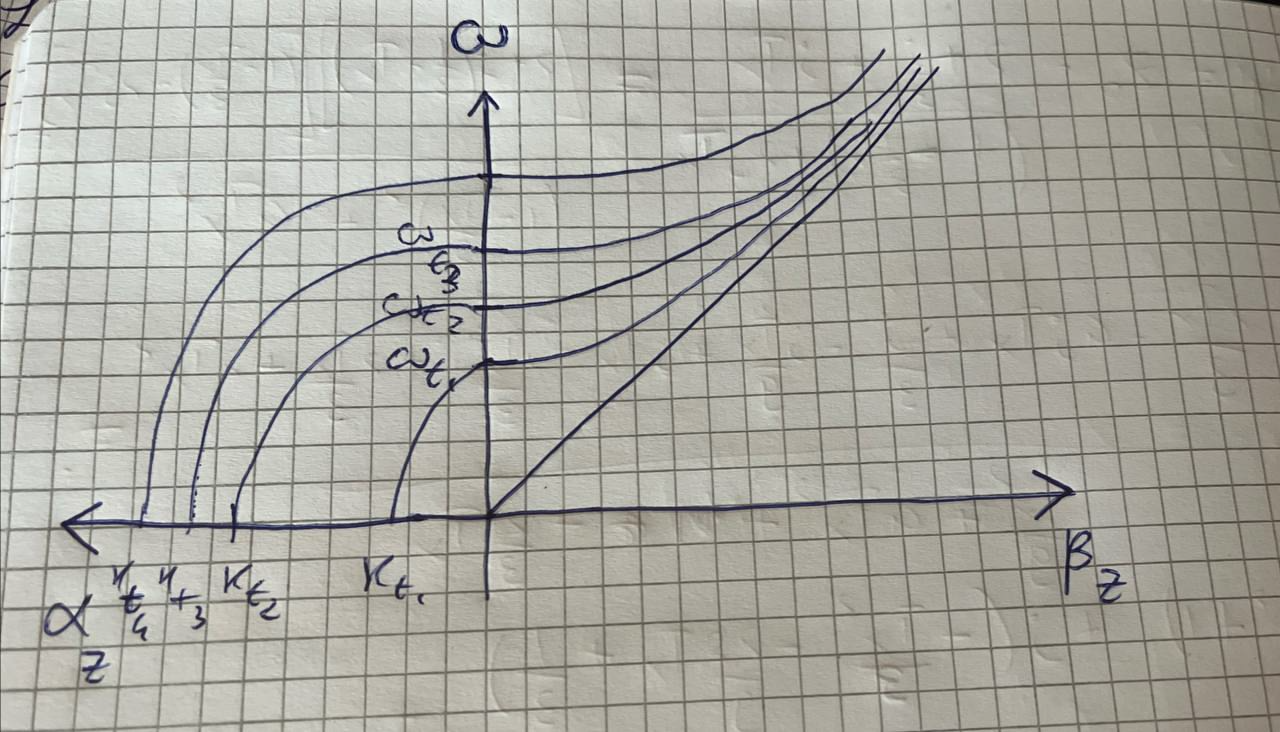
\includegraphics[width=0.7\linewidth]{img/Chapter_three/Chapt3img1.png}
    \end{figure}
    \\ \\
    Come fare per contenere la distorsione modale? Se c'è  propagazione TEM non ci sono problemi, basta 
    restare al di sotto della frequenza di cutoff fondamentale. Se però ci sono solo TE e TM? Ci sono un'infinità numerabile di modi
    TE e TM all'interno delle guide, seppur con le loro intensità variabili. Se si parte con un solo modo e si becca una discontinuità,
    anche di entità lieve, questi si mischiano fra loro distorcendo il segnale facendo variare lo spetto di frequenza. \\
    La velocità dell'inviluppo del pacchetto d'onda, ovvero la \textbf{velocità di fase}, per segnali a banda stretta è diversa da quella di fase. 
    Torneremo a parlare di distorsione nelle prossime lezioni.

\section{Guida d'onda rettangolare}
    Il modo a cui è associata la frequenza di taglio minore è detto \textbf{modo fondamentale}. In questa 
    sezione ricaviamo il primo modo fondamentale per le guide rettangolari cavi, attraverso le quali non c'è propagazione TEM. 
    Per far ciò, occorre determinare $\Phi$ per i modi TM e $\Psi$ per quelli TE. \\ \\
    Consideriamo una sezione rettangolare di lati $a$ e $b$, con $a>b$ ed orientiamone i lati con normali come in figura:
    \begin{figure}[h!]
        \center  
        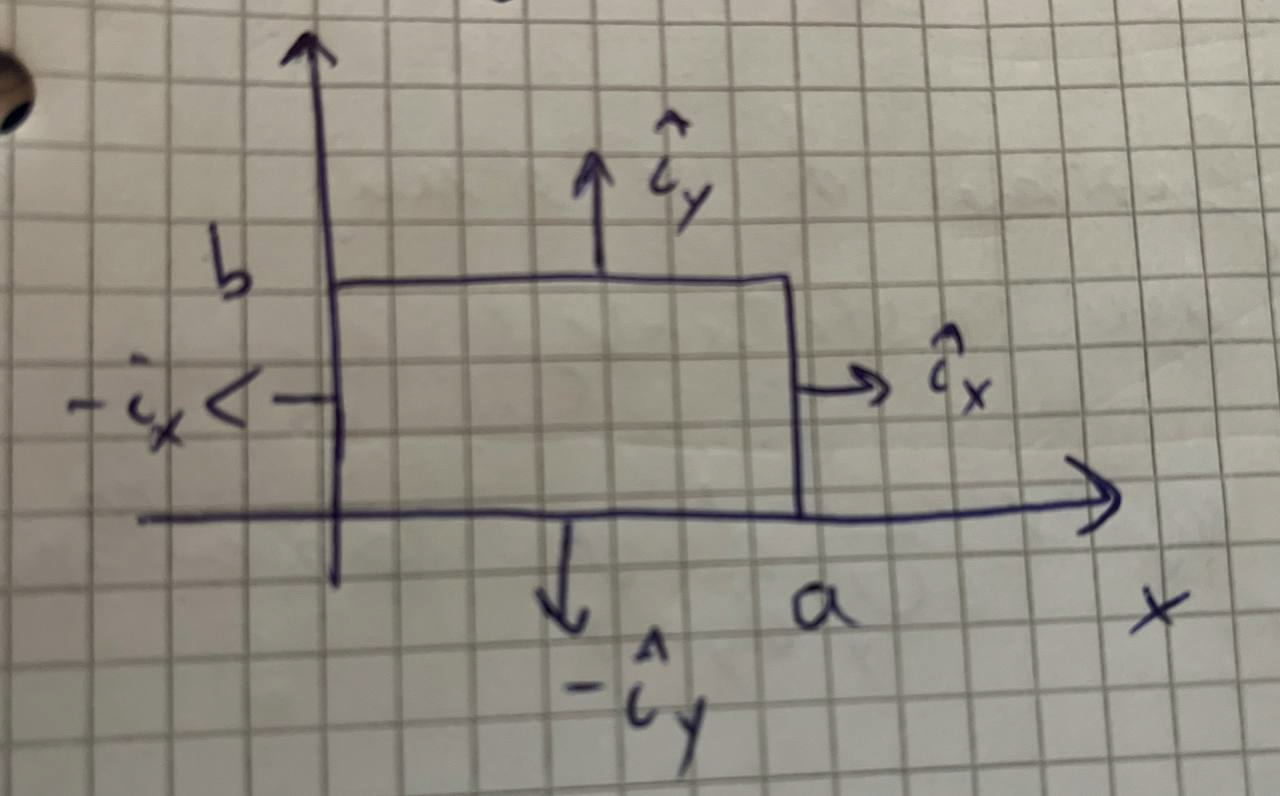
\includegraphics[width=0.6\linewidth]{img/Chapter_three/Chapt3img2.png}
    \end{figure}
    \\ Per i TE risulta:
    \begin{equation}
        \begin{cases}
            \nabla_{t} ^{2} \Psi + k_{t} ^{2} \Psi = 0 \\
            \frac{\partial}{\partial n} \Psi|_{\mathcal{C}} = 0
        \end{cases}
    \end{equation}
    dove $\displaystyle \frac{\partial}{\partial n}$ è l'operatore di derivata rispetto alla normale e $\mathcal{C}$ il perimetro
    della sezione.\\
    Riscriviamo esplicando il laplaciano:
    \begin{equation}
        \label{eqn:mi_serve6}
        \begin{cases}
            \displaystyle \frac{\partial ^{2}}{\partial x^{2}}\Psi + \frac{\partial ^{2}}{\partial y^{2}}\Psi + k_{t} ^{2} \Psi = 0 \\
            \displaystyle \frac{\partial}{\partial n} \Psi|_{\mathcal{C}} = 0
        \end{cases}
    \end{equation} \\
    La seconda equazione delle (\ref{eqn:mi_serve6}) è una condizione al contorno, scomponibile in quattro condizioni, una per ogni lato.
    In accordo a come abbiamo posto le normali possiamo scrivere:
    \begin{equation}
        \frac{\partial}{\partial x} \Psi|_{x=a} = - \frac{\partial}{\partial x}\Psi|_{x=0} = -\frac{\partial}{\partial y}|_{y=0}\Psi = \frac{\partial}{\partial y}|_{y=b} \Psi = 0
    \end{equation}
    Supponiamo che $\Psi(x,y)$ sia fattorizzabile come
    \begin{equation}
        \Psi(x,y) = \Psi_{x}(x)\Psi_{y}(y)
    \end{equation} 
    Allora si può scrivere, in accordo alla prima equazione delle (\ref{eqn:mi_serve6})
    \begin{equation}
        \Psi_{y}\frac{d ^{2}}{d x^{2}}\Psi_{x} + \Psi_{x}\frac{d ^{2}}{d y^{2}}\Psi_{y} + k_{t} ^{2} \Psi_{x}\Psi_{y} = 0
    \end{equation}
    Dividendo per $\Psi=\Psi_{x}\Psi_{y}$ si ottiene
    \begin{equation}
        \frac{1}{\Psi_{x}}\frac{d}{dx^{2}}\Psi_{x}+\frac{1}{\Psi_{y}}\frac{d}{dy^{2}}\Psi_{y} = -k_{t} ^{2}
    \end{equation}
    La somma di una funzione di $x$ ed una di $y$ deve essere pari ad una costante, dunque le singole funzioni sono anche loro costanti. Posto allora:
    \begin{equation}
        -k_{x} ^{2} = \frac{1}{\Psi_{x}}\frac{d}{dx^{2}}\Psi_{x} \qquad -k_{y} ^{2} = \frac{1}{\Psi_{y}}\frac{d}{dy^{2}}\Psi_{y}
    \end{equation}
    ricaviamo un espressione molto più pulita:
    \begin{equation}
        \begin{cases}
            k_{x} ^{2}+k_{y} ^{2} = k_{t} ^{2} \\
            -k_{x} ^{2} = \frac{1}{\Psi_{x}}\frac{d}{dx^{2}}\Psi_{x} \\
            -k_{y} ^{2} = \frac{1}{\Psi_{y}}\frac{d}{dy^{2}}\Psi_{y}
        \end{cases}
        \implies
        \begin{cases}
            k_{x} ^{2}+k_{y} ^{2} = k_{t} ^{2} \\
            \frac{d}{dx^{2}}\Psi_{x}+k_{x}^{2}\Psi_{x} = 0 \\
            \frac{d}{dy^{2}}\Psi_{y}+k_{y}^{2}\Psi_{y} = 0
        \end{cases}
    \end{equation}
    Le ultime due equazioni hanno la stessa forma di quella di un oscillatore armonico, dunque le 
    soluzioni sono seni e coseni. Scriviamo allora
    \begin{equation}
        \begin{cases}
            \displaystyle \Psi_{x}(x) = A_{x}\cos(k_{x}x)+B_{x}\sin(k_{x}x) \\
            \displaystyle \Psi_{y}(y) = A_{y}\cos(k_{y}y)+B_{y}\sin(k_{y}y)
        \end{cases}
    \end{equation}
    Applichiamo le condizioni al contorno. Partiamo da quella per $x=0$:
    \begin{equation}
        \frac{\partial}{\partial x}\Psi|_{x=0} =\Psi_{y} \frac{d}{dx}\Psi|_{x=a} \qquad \forall y \in [0, b] 
    \end{equation}
    La soluzione $\Psi_{y}=0$ è banale, dunque la derivata deve essere nulla. Allora $\Psi_{x}$ è costante sul bordo. 
    Lo stesso ragionamento può essere fatto per la condizione al bordo $x=a$. Per $x=0$, sostituendo nella soluzione generale, si ottiene:
    \begin{equation}
        \frac{d}{dx}\Psi_{x}|_{x=0} = B_{x}k_{x} = 0
    \end{equation}
    mentre per $x=a$
    \begin{equation}
        \frac{d}{dx}\Psi|_{x=a} = -A_{x}k_{x}\sin(ak_{x})
    \end{equation}
    Dunque la condizione da soddisfare è una tra le due a seguire:
    \begin{equation}
        B_{x}k_{x} = 0 \qquad \textrm{oppure} \qquad k_{x}=\frac{n\pi}{a}
    \end{equation}
    Per $\Psi_{y}$ il ragionamento è analogo e occorre soddisfare una delle due
    \begin{equation}
        B_{y}k_{y} = 0 \qquad \textrm{oppure} \qquad k_{y} = \frac{m \pi}{b}
    \end{equation}
    Abbiamo un'espressione per $k_{x}$ e $k_{y}$, che possiamo sostituire nell'integrale generale
    \begin{equation}
        \begin{cases}
            \displaystyle \Psi_{x}(x) = A_{x}\cos(\frac{n \pi}{a}x)+B_{x}\sin(\frac{n \pi}{a}x) \\
            \\
            \displaystyle \Psi_{y}(y) = A_{y}\cos(\frac{m\pi}{b}y)+B_{y}\sin(\frac{m\pi}{b}y)
        \end{cases}
    \end{equation}
    Ipotizzando che $k_{x} \neq 0  \ (n \neq 0)$ deve risultare $B_{x}=0$ e di conseguenze
    \begin{equation}
        \Psi_{x}(x)=A_{x}\cos(\frac{n\pi}{a}x)
    \end{equation}
    Se $k_{x}=0$ il seno si annulla e si ha la stessa espressione, quindi $B_{x}=0$ sempre. Il ragionamento analogo 
    per $\Psi_{y}$ ci permette di scrivere 
    \begin{equation}
        \label{eqn:base_soluzioniTE}
        \begin{cases}
            \Psi_{x}(x) = A_{x}\cos(\frac{n \pi}{a}x)  \\
            \Psi_{y}(y) = A_{y}\cos(\frac{m \pi}{b}y) 
        \end{cases}
        \qquad n, m \in \mathbb{N}_{0} \times \mathbb{N}_{0} - \{0, 0\}
    \end{equation}
    Perché la condizione su $m,n $? Posto $A_{x}, A_{y} \neq 0$, altrimenti si avrebbe la soluzione banale, escludiamo anche il caso per il quale $\{n,m\} = \{0,0\}$,
    perché sennò si avrebbe $\Psi_{x}$ e $\Psi_{y}$ costanti, altra soluzione banale. Inoltre poiché il coseno è una funzione pari, lo spazio $\mathbb{Z} \times \mathbb{Z}$
    contiene la stessa informazione di quello $N_{0} \times N_{0}$. 
    \\ Le (\ref{eqn:base_soluzioniTE}) generano una base per le soluzioni TE all'interno della guida rettangolare. Tale base è costituita dai modi 
    identificati dagli indici $n$ ed $m$. \\
    Utilizziamo la relazione che abbiamo trovato in precedenza per identificare la costante di propagazione del modo $\textrm{TE}_{m,n}$:
    \begin{equation}
        k_{x} ^{2} +k_{y} ^{2}= k_{t} ^{2} \implies k_{t_{n,m}} = \sqrt{(\frac{n \pi}{a})^{2}+(\frac{m \pi}{b})^{2}}
    \end{equation}
    Per identificare il modo fondamentale, bisogna trovare il $k_{t_{n,m}}$ più piccolo. Se $a>b$ è immediato verificare che questo corrisponde 
    a $k_{t_{1,0}}$:
    \begin{equation}
        k_{t_{1,0}} = \frac{\pi}{a} < k_{t_{0,1}} = \frac{\pi}{b}
    \end{equation}
    Da cui ricaviamo il relativo modo
    \begin{equation}
        \Psi_{1,0} = A_{1,0}\cos(\frac{\pi}{a}x)
    \end{equation}
    con $A_{1,0}$ costante arbitraria in virtù della fattorizzazione. La scelta più semplice ricade nel porre 
    $A_{1,0}$ tale da normalizzare il modulo quadro della $\Psi$:
    \begin{equation}
        ||\Psi_{1,0}|| ^{2} = A_{1,0} ^{2} \int_{0} ^{a} \int_{0} ^{b} \cos^{2}(\frac{\pi}{a}x)dxdy = 1 \implies A_{1,0} = \sqrt{\frac{2}{ab}}
    \end{equation}
    Conoscendo $\Psi_{1,0}$ si ricavano le relative funzioni vettoriali di modo
    \begin{equation}
        \underline{h}_{1,0} = -\frac{1}{k_{t_{1,0}}} = \sqrt{\frac{2}{ab}} \sin(\frac{\pi}{a}x)\underline{i}_{x}
    \end{equation}
    avendo tenuto conto che $\nabla_{t} = (\frac{\partial}{\partial x} \ \ \frac{\partial}{\partial y})$. \\
    Ricaviamo anche $\underline{e}_{1,0}$
    \begin{equation}
        \underline{e}_{1,0} = \underline{h}_{1,0} \times \underline{i}_{z} = \sqrt{\frac{2}{ab}} = \sin(\frac{\pi}{a}x)\underline{i}_{x} \times \underline{i}_{z} = -\sqrt{\frac{2}{ab}}\sin{\frac{\pi}{a}x}\underline{i}_{y}
    \end{equation}
    perché $\underline{i}_{x}\times\underline{i}_{z} = - \underline{i}_{y}$. Infine si ricava 
    la componente tangete di $\underline{H}$:
    \begin{equation}
        \underline{H}_{z} = \frac{V(z)}{j \omega \mu}k_{t_{1,0}} \cdot \Psi_{1,0} = \frac{V(z)}{j \omega \mu} \frac{\pi}{a}\sqrt{\frac{2}{ab}}\cos(\frac{\pi}{a}x)
    \end{equation} \\ \\ \\ \\
    Proseguiamo analogamente per ricavare l'espressione per i modi TM. Sappiamo che vale
    \begin{equation}
        \begin{cases}
            \frac{\partial ^{2}}{\partial x^{2}}\Phi + \frac{\partial ^{2}}{\partial y^{2}}\Phi +k_{t} ^{2}\Phi = 0 \\
            \Phi|_{\mathcal{C}} = 0
        \end{cases}
    \end{equation}
    Supponiamo come prima che $\Phi(x,y) = \Phi_{x}(x)\Phi_{y}(y)$. Allo stesso modo, arriviamo a determinare
    \begin{equation}
        \begin{cases}  
        \frac{d ^{2}}{dx ^{2}}\Phi_{x}+k_{x} ^{2}\Phi_{x} = 0 \\
        \frac{d^{2}}{dy^{2}}\Phi_{y}+k_{y} ^{2}\Phi_{y} = 0 \\
        k_{x} ^{2}+k_{y} ^{2}=k_{t} ^{2}
        \end{cases}
    \end{equation}
    Che corrispondono agli integrali generali
    \begin{equation}
        \begin{cases}
            \displaystyle \Phi_{x}(x) = A_{x}\cos(k_{x}x)+B_{x}\sin(k_{x}x) \\
            \displaystyle \Phi_{y}(y) = A_{y}\cos(k_{y}y)+B_{y}\sin(k_{y}y)
        \end{cases}
    \end{equation}
    Applicando le condizioni al contorno si ottiene
    \begin{equation}
        \Phi_{x} (0) = 0 \implies A_{x} = 0 \qquad \Phi_{y}(0) = 0 \implies A_{y} = 0
    \end{equation}
    \begin{equation}
        \Phi_{x}(a) = 0 \implies k_{x} = \frac{n\pi}{a} \qquad \Phi_{y}(b)=0 \implies k_{y} = \frac{m \pi}{b}  
    \end{equation}
    Ottenendo in definitiva
    \begin{equation}
        \Phi_{n,m} (x,y) = B_{x_{n}}B_{y_{m}}\sin(\frac{n \pi}{a}x)\sin(\frac{m \pi}{b}y) \qquad n, m > 0
    \end{equation}
    A differenza del caso TE, il modo TM dipende dal prodotto di due seni e dunque $n$ ed $m$ non possono esser nulli,
    altrimenti si avrebbe soluzione banale! \\
    Ricaviamo il la costante di propagazione più piccola
    \begin{equation}
        k_{t_{1,1}} ^{TM}= \pi\sqrt{\frac{1}{a}+\frac{1}{b}} \implies \Phi_{1,1} = B_{11}\sin(\frac{\pi}{a}x)\sin(\frac{\pi}{b}y)
    \end{equation}
    la quale è sicuramente maggiore di $k_{1,0} ^{TE}$. Allora \textbf{in una guida rettangolare il modo fondamentale è il TE 10}.\footnote{leggasi "uno zero"}
    \\ \\ 
    Affrontiamo ora il tema su come selezionare $a$ e $b$ all'interno di una guida rettangolare. Sappiamo che la frequenza di taglio indicizzata tramite $n$ ed $m$ è data da 
    \begin{equation}
        \omega_{t_{m,n}} = c k_{t_{m,n}} = c \sqrt{(\frac{n \pi}{a})^{2}+(\frac{m \pi}{b})^{2}} 
    \end{equation}
    Il fondamentale è $TE_{10}$ con relativa frequenza di taglio $\omega_{t_{10}} ^{TE} = c\frac{\pi}{a}$. Il secondo modo fondamentale sarà uno fra i seguenti
    \begin{equation}
        \omega_{20} ^{TE} = 2 \frac{c\pi}{b} \qquad \omega_{01} ^{TE} = \frac{c\pi}{b} \qquad \omega_{11} ^{TE} = c\sqrt{(\frac{\pi}{a})^{2}+(\frac{\pi}{b})^{2}} = \omega_{11} ^{TM}
    \end{equation}
    Possiamo scartare a priori la $\omega_{11} ^{TE}=\omega_{11} ^{TM}$ perché è sicuramente maggiore delle altre due. Se $b > a/2$ la $\omega_{01} ^{TE}$ è la fondamentale,
    altrimenti è la $\omega_{20} ^{TE}$, dunque il problema si riduce alla scelta dell rapporto fra $a$ e $b$. \\
    È di nostro interesse che la banda, identificata tra la fondamentale e la seconda frequenza di taglio, sia maggiore possibile. Per far ciò, conviene scegliere $b \leq a/2$. Dal punto di vista teorico l'ideale 
    sarebbe proprio $b=a/2$, ma per tener conto delle imperfezioni si sceglie poco più piccola per star sicuri. Il motivo per il quale si sceglie $a/2$ è dovuto al fatto che, come abbiamo visto poco sopra, il fattore geometrico 
    per i campi va come $\sqrt{\frac{2}{ab}}$, dunque aumenta al diminuire di $b$, aumentando la potenza dissipata.


    \section{Soluzione TEM}
        Nel caso TEM, la situazione è la seguente
        \begin{figure}[h!]
            \center  
            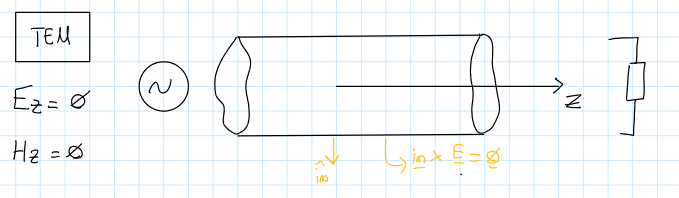
\includegraphics[width=0.6\linewidth]{img/Chapter_three/Chapt3img3.png}
        \end{figure}
        \newpage 
        Per i TEM, valgono le seguenti
        \begin{equation}
            \begin{cases}
                \displaystyle -\frac{d}{dz}V = jkZ_{0}I \\
                \displaystyle -\frac{d}{dz}I = j \frac{k}{Z_{0}} V
            \end{cases} \qquad 
            \begin{cases}
                k = \omega \sqrt{\varepsilon \mu} \\
                \displaystyle Z_{0} = \frac{\zeta}{A} \\
                \displaystyle \zeta = \sqrt{\frac{\mu}{\varepsilon}}
            \end{cases} \qquad 
            \begin{cases}
                \underline{e} = A \underline{h} \times \underline{i}_{z} \\
                A \underline{h} = \underline{i}_{z} \times \underline{e}
            \end{cases}
        \end{equation}
        Le equazioni di Markuvitz-Schwinger in questo caso avevano la forma
        \begin{equation}
            \begin{cases}
            \displaystyle -\frac{\partial}{\partial z}\underline{E}_{t} = j \omega \mu \underline{H}_{t} \times \underline{i}_{z} \\
            \displaystyle -\frac{\partial}{\partial z}\underline{H}_{t} = j \omega \varepsilon \underline{i}_{z} \times \underline{E}_{t} \\
            0 = \nabla_{t} \cdot (\underline{i}_{z} \times \underline{E}_{t}) \\
            0 = \nabla_{t} \cdot (\underline{H}_{t}\times \underline{i}_{z})
            \end{cases}
        \end{equation}
        Le prime due equazioni le abbiamo usate per le linee, dunque useremo le ultime due per trovare l'espressione di $\underline{e}$ ed $\underline{h}$. Avevamo visto con la (\ref{eqn:campi_irrotazionali_indivergenti_TEM}) che
        $\underline{e}$ ed $\underline{h}$ sono nel caso TEM sia irrotazionali che indivergenti. Se assumiamo che il volume all'interno del quale stiamo risolvendo il problema di campo sia semplicemente connesso, possiamo affermare 
        \begin{equation}
            \begin{cases}
                \nabla_{t} \times \underline{e}, \ \nabla_{t} \times \underline{h} = 0 \\
                V \ \textrm{semplicemente connesso}
            \end{cases} 
            \implies
            \underline{e} \textrm{ ed } \underline{h} \textrm{ sono campi conservativi} 
        \end{equation}
        Dire che il campo è conservativo corrisponde a dire che \textbf{esiste una funzione scalare tale per cui il campo è esprimibile come l'opposto del gradiente di tale funzione scalare}. \newpage 
        Posizionandoci ad una sezione della guida in tal modo
        \begin{figure}[h!]
            \center  
            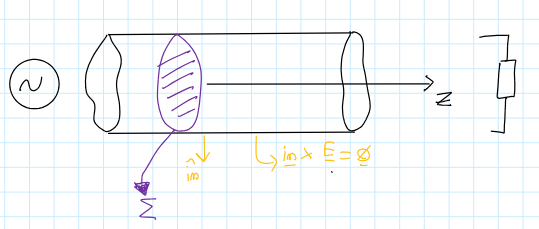
\includegraphics[width=0.6\linewidth]{img/Chapter_three/Chapt3img4.png}
        \end{figure}
        $\underline{h}$ ed $\underline{e}$ vivono in $\Sigma$, per cui bisogna verificare che $\Sigma$ sia un dominio semplicemente connesso\footnote{Ha senso parlare di dominio bidimensionale e non tridimensionale perché le funzioni vettoriali di modo
        sono definite sulle due dimensioni tangenti $x$ ed $y$}; se consideriamo la sezione di un cavo coassiale, è istantaneo verificare che il dominio non è semplicemente connesso. Poiché vale
        \begin{equation}
            \oint_{C} = \underline{E} \cdot \underline{i}_{l}dl = - j \omega \mu \iint_{S_{C}} \underline{H} \cdot \underline{i}_{n} dS
        \end{equation}
        avendo scelto una curva $C$ sulla corona circolare\footnote{la zona fra anima e calza} del cavo, la quale racchiude area $S_{C}$.
        Per il cavo coassiale (così come ogni guida) $\underline{i}_{n}=\underline{i}_{z}$ per cui $\underline{H}\cdot \underline{i}_{n} = H_{z} = 0$ nel caso TEM.
        Dunque si può scrivere 
        \begin{equation}
            \oint_{C} \underline{E} \cdot \underline{i}_{l} dl = -j \omega \mu \iint_{S_{C}} H_{z} dS = 0 \implies \oint_{C} \underline{E} \cdot \underline{i}_{l} dl = 0 
        \end{equation} 
        dunque $\underline{E}$ è un campo conservativo. Dato che $E_{z}= 0$ si può scrivere la circuitazione di $\underline{E}$ considerando solo il contributo tangente
        \begin{equation}
            \oint_{C} \underline{E}_{t} \cdot \underline{i}_{l} dl = V(z) \oint_{C} \underline{e} (\underline{r}_{t}) \cdot \underline{i}_{l} dl = 0 \implies \oint_{C} \underline{e} (\underline{r}_{t}) \cdot \underline{i}_{l} dl = 0
        \end{equation}
        assumendo che $V(z) \neq 0$, altrimenti avremmo solo la soluzione banale. Poiché la scelta di $C$ è arbitraria, l'integrale è nullo per ogni curva e dunque $\underline{e}$ è un campo conservativo. \\
        Sia $\varphi$ il potenziale scalare di $\underline{e}$, l'irrotazionalità di $\underline{e}$ nel caso di conservatività porta la stessa informazione di $\underline{e} = - \nabla_{t} \varphi$
        \begin{equation}
            \begin{cases}
                \nabla_{t} \cdot \underline{e} = 0 \\
                \underline{e} = - \nabla_{t} \varphi
                \end{cases} \implies 
                0 = \nabla_{t} \underline{e} = - \nabla_{t} \cdot \nabla_{t} \varphi \implies \nabla_{t} ^{2} \varphi = 0 
        \end{equation}
        Per ricavare $\underline{e}$ occorre risolvere l'equazione di Laplace che abbiamo appena ricavato. \\
        Per $\underline{h}$ il discorso \textit{dovrebbe} essere analogo. Selezionata una curva arbitraria $C$ all'interno della corona circolare del cavo coassiale possiamo scrivere, nel caso TEM dove $E_{z} = 0$
        \begin{equation}
            \oint_{C} \underline{H} \cdot \underline{i}_{l} dl = j \omega \varepsilon \iint_{S_{C}} \underline{E} \cdot \underline{i}_{n} dS + i (\underline{\underline{S_{C}}}) =
            j \omega \varepsilon \iint_{S_{C}} i (\underline{\underline{S_{C}}})
        \end{equation}
        Poiché c'è la corrente, non è possibile dire subito che $\underline{h}$ è conservativo, per cui si ricava $\underline{e}$ e poi $\underline{h}$. Occorre risolvere 
        \begin{equation}
            \begin{cases}
                \underline{e} = - \nabla_{t} \varphi \\
                \nabla_{t} \varphi = 0
            \end{cases}
        \end{equation}
        la quale ha infinite soluzioni, a meno che non vengano specificate le condizioni al contorno.
        \begin{figure}[h!]
            \center  
            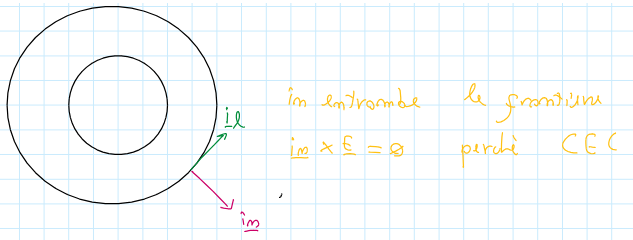
\includegraphics[width=0.6\linewidth]{img/Chapter_three/Chapt3img5.png}
        \end{figure}
        Le condizioni al contorno, considerando il CEP, sono
        \begin{equation}
            0 = \underline{i}_{n} \times \underline{E}|_{\partial \Sigma} = \underline{i}_{n} \times \underline{E}_{t}|_{\partial \Sigma} = V(z)\underline{i}_{n} \times \underline{e}(\underline{r}_{t})|_{\partial \Sigma}
        \end{equation}
        Posto $V(z) \neq 0$ risulta
        \begin{equation}
            0 = \underline{i}_{n} \times \underline{e}|_{\partial \Sigma}  = - \underline{i}_{n} \times \nabla_{t} \varphi |_{\partial \Sigma}
        \end{equation}
        Considerato il versore $\underline{i}_{l}$ tangente e quello longitudinale $\underline{i}_{z}$ la situazione è questa
        \begin{figure}
            \center  
            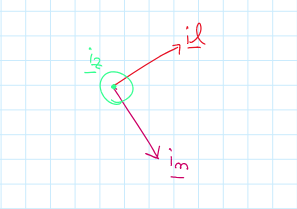
\includegraphics[width=0.6\linewidth]{img/Chapter_three/Chapt3img6.png}
        \end{figure}
        Dunque, forti del fatto che $\underline{i}_{n} = \underline{i}_{l} \times \underline{i}_{z}$
        \begin{equation}
            \underline{i}_{n} \times \nabla_{t} \varphi |_{\partial \Sigma} = (\underline{i}_{l} \times \underline{i}_{z}) \times \nabla_{t} \varphi |_{\partial \Sigma} = (\underline{i}_{l} \cdot \nabla_{t} \varphi) \underline{i}_{z} -
            (\underline{i}_{z} \cdot  \nabla_{t}\varphi) \cdot \underline{i}_{l}|_{\Sigma} = (\underline{i}_{l} \cdot \nabla_{t} \varphi ) \cdot \underline{i}_{z}
        \end{equation}
        dato che $\nabla_{t} \varphi = - \underline{e} \implies \nabla_{t}\varphi|_{z} \cdot \nabla_{t} \varphi = 0$. Si scrive in definitiva 
        \begin{equation}
            \underline{i}_{l} \nabla_{t} \varphi |_{\partial \Sigma} = \frac{\partial \varphi}{\partial l}|_{\Sigma} = 0
        \end{equation}
        perché il prodotto gradiente per versore è la derivata direzionale in direzione del versore. \\ 
        Allora occorre cercare una $\varphi$ che soddisfi:
        \begin{equation}
            \begin{cases}
                \nabla_{t} ^{2} \varphi = 0 \\
                \displaystyle \frac{\partial \varphi}{\partial l}|_{\Sigma} = 0
            \end{cases}
        \end{equation}
        Il fatto che la derivata di $\varphi$ lungo la direzione  $\underline{i}_{l}$ sia nulla \textbf{non implica che sia costante lungo tale direzione} a meno che che il dominio non sia connesso,
        perché se così non fosse questa potrebbe variare al di fuori del dominio e rimanere costante solo all'interno di esso. La frontiera di un cavo coassiale, come sappiamo, non è connessa.\\
        \begin{figure}[h!]
            \center  
            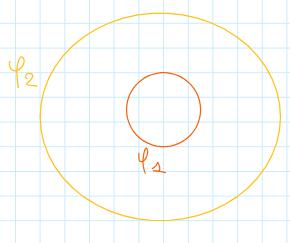
\includegraphics[width=0.6\linewidth]{img/Chapter_three/Chapt3img7.png}
        \end{figure}
        \\ Ci sono due valori diversi di $\varphi$ sulla frontiera non connesso del cavo coassiale, le quali però sono costanti. Se tali costanti sono diverse ciò risulta comodo perché significa che ci sarà 
        una differenza di potenziale fra i conduttori. \newpage 
        Consideriamo ora un domino del genere
        \begin{figure}[h!]
            \center  
            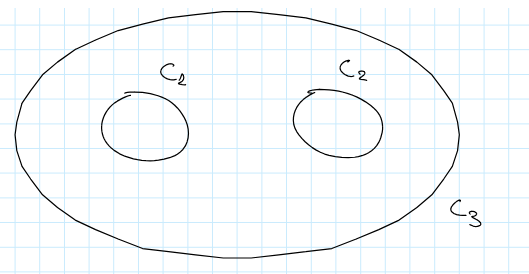
\includegraphics[width=0.6\linewidth]{img/Chapter_three/Chapt3img8.png}
        \end{figure} \\
        Ci chiediamo quanti modi TEM si propagano in una struttura guidante che ha una sezione come quella in figura. Ricordiamo che $\underline{e}$ e $\varphi$ sono quantità complesse, i casi da considerare sono tre,
        cioè che si propagahi un modo su una delle superfici laterali (ognuna ha il suo "cerchio" in sezione, dunque i due interni e quello esterno). Sfruttando la linearità del mezzo, si può scrivere la $\varphi$ totale come somma 
        di tutti e tre i contributi dei tre conduttori
        \begin{equation}
            \varphi = c_{1}\varphi_{1}+c_{2}\varphi_{2}+c_{3}\varphi_{3}
        \end{equation} 
        La $\varphi_{1}$ può essere complessa, ma le $\varphi_{2}$ e $\varphi_{3}$ sono reali (perché ???) dunque la condizione per la $\varphi_{1}$ assume la forma
        \begin{equation}
            \begin{cases}
                \nabla_{t} ^{2} \varphi_{1R} = 0 \\
                \nabla_{t} ^{2} \varphi_{1I} = 0
            \end{cases}
        \end{equation}
        cioè le componenti di $\varphi_{1}$ sono due funzioni armoniche reali, così come lo sono $\varphi_{2}$ e $\varphi_{3}$. Le funzioni armoniche reali sono costrette ad assumere massimo e minimo sulla frontiera.
        Applichiamo la sovrapposizione degli effetti: quando agisce solo $\varphi_{1}$, se questa assume massimo sulla frontiera e minimo sull'altra, allora la parte immaginaria è zero (dubbio, chiedi al professore). Dato 
        che lafrontiera è $1$ o $0$ si ottiene su tutta la superficie $S$:
        \begin{equation}
            \varphi_{S} = \varphi_{1}+\varphi_{2}+\varphi_{3} \qquad \nabla_{t} ^{2} \varphi_{S} = 0
        \end{equation} 
        Poiché la somma in ogni frontiera deve fare $\varphi_{S} = 1$ risulta
        \begin{equation}
            \varphi_{1}+\varphi_{2}+\varphi_{3} = 1 \implies \varphi_{3} = 1- \varphi_{2} - \varphi_{2} \implies \varphi = (1-c_{3})\varphi_{1}+(c_{2}-c_{3})\varphi_{2}+c_{3}
        \end{equation}
        dunque per tre contorni servono due modi TEM. In generale, per un dominio con molteplcità $n$ si propagano $n-1$ modi TEM. Il problema del tubo cavo allora non ammette modo TEM e per frequenze 
        basse del segnale occorrerebbero modi TE e TM con frequenze di taglio molto basse con sezioni di tubo enorme. \newpage
        \subsection{Il cavo coassiale}
        Il cavo coassiale è una struttura guidante che consta di due conduttori che sono, per l'appunto, coassiali. Ha doppia molteplcità e dunque al suo interno si 
        propaga un singolo modo TEM. Per studiare il comportamento di tale modo, consideriamo una sezione coassiale di raggi $a$ (conduttore interno) e $b$ (conduttore esterno). Sia $P = (r, \vartheta)$ il 
        generico punto all'interno della sezione e $\varphi = \varphi(x,y) \in \mathbb{R}$
        \begin{figure}[h!]
            \center  
            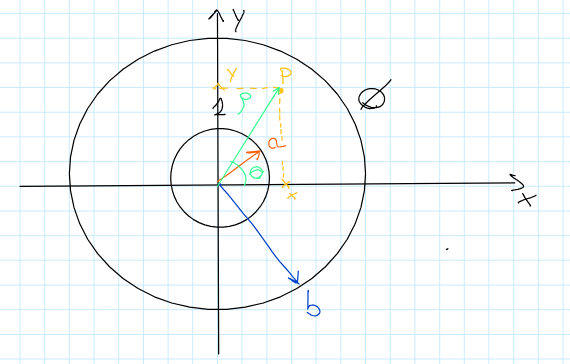
\includegraphics[width=0.7\linewidth]{img/Chapter_three/Chapt3img9.png}
        \end{figure}
        Il laplaciano ha la forma
        \begin{equation}
            \nabla_{t} ^{2} \varphi = \frac{\partial ^{2}}{ \partial x^{2}}\varphi + \frac{\partial ^{2}}{\partial y ^{2}}\varphi = 0
        \end{equation}
        Conviene esprimerlo in coordinate polari, dunque
        \begin{equation}
            \varphi = \varphi(\rho, \vartheta) = \varphi(\rho) = 
        \end{equation}
        dove l'ultimo passaggio è giustificato dal fatto che, poiché la struttura è simmetrica rispetto ad una rotazione attorno al suo asse, anche la soluzione erediti tale simmetria, dipendendo 
        solo da $\rho$. Allora scriviamo:
        \begin{equation}
            \nabla_{t} ^{2} \varphi = \frac{1}{\rho} \frac{d}{d\rho} [\rho \frac{d}{d \rho} \varphi(\rho)] = 0 \qquad \rho \in [a, b] \implies \rho \frac{d}{d \rho} \varphi = c_{1} = \textrm{ costante }
        \end{equation}
        \begin{equation}
            \implies \frac{d \varphi}{d \rho} = \frac{c_{1}}{\rho} \implies \varphi = c_{1} \ln (\rho) + c_{2}
        \end{equation}
        Le condizioni al contorno da imporre sono
        \begin{equation}
            \begin{cases}
            \varphi (a) = 1 \\
            \varphi (b) = 0
            \end{cases}
        \end{equation}
        dove $1$ è stata imposta in modo arbitrario, ma in generale il valore sulla superficie piccolina è $c_{1}$.
        Per cui
        \begin{equation}
            \begin{cases}
                c_{1} \ln (a)+c_{2} = 1 \\
                c_{1} \ln (b)+c_{2} = 0
            \end{cases}
        \end{equation}
        Sostituendo
        \begin{equation}
            \begin{cases}
            c_{1}(\ln(a)-\ln(b)) = c_{1} \ln(\frac{a}{b})= 1 \\
            c_{2} = -c_{1}\ln(b)
            \end{cases} \implies 
            \begin{cases}
            \displaystyle    c_{1} = \frac{1}{\ln (\frac{a}{b})} \\
            \displaystyle    c_{2} = -\frac{1}{\ln(\frac{a}{b})}\ln(b)
            \end{cases}
        \end{equation}
        Allora per il campo $\underline{e}$ possiamo scrivere
        \begin{equation}
            \underline{e} = - \nabla_{t} \varphi = - \frac{d}{d\rho} \varphi \cdot \underline{i}_{\rho} = - \frac{c_{1}}{\rho} \underline{i}_{\rho} = - \frac{1}{\displaystyle \ln(\frac{a}{b}) \rho} \underline{i}_{\rho}
        \end{equation}
        \begin{equation}
        \implies \underline{e} = \frac{1}{\ln (\frac{b}{a})\rho} \cdot \underline{i}_{\rho}
        \end{equation}
        Data la struttura del cabo coassiale ($b>a$) il logaritmo a denominatore è positivo e dunque il campo $\underline{e}$ viene irradiato dalla sezione piccola a quella grande, in modo radiale.
        \\ L'espressione del campo magnetico viene ricavata dalla relazione da cui siamo partiti
        \begin{equation}
        \underline{h} = \frac{1}{A} \underline{i}_{z} \times \underline{e} = \frac{1}{A} \underline{i}_{z} \times (\frac{1}{\ln (\frac{b}{a})}\rho)
        \end{equation}
        \begin{figure}[h!]
        \center  
        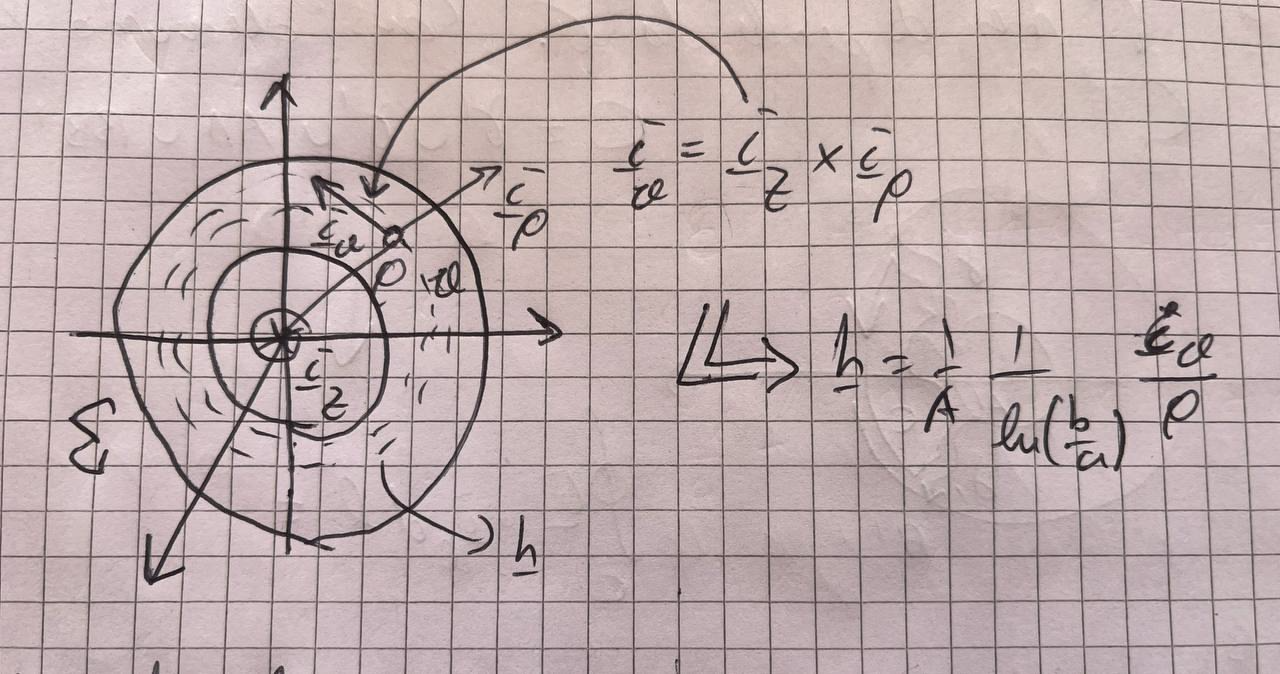
\includegraphics[width=0.5\linewidth]{img/Chapter_three/Chapter3img10.png}
        \end{figure} \\
        Le linee di campo magnetico sono azimutali, circoferenze con centro nella direzione di $\underline{i}_{z}$. \\
        Dimostriamo ora che nel caso TEM le funzioni scalari di modo corrispondono alla tensione e alla corrente.
        La tensione $\mathcal{V}$ tra due punti corrisponde alla circuitazione del campo elettrico lungo la curva che unisce tali punti
        \begin{equation}
        \mathcal{A, B, \gamma} = \int_{A} ^{B} \underline{E} \cdot \underline{i}_{l} dl
        \end{equation}
        Il nostro scopo è far vedere che, fissato $z$, la funzione scalare di modo $V(z)$ è costante rispetto alla scelta di 
        due punti $A$ e $B$, uno su ogni conduttore, e rispetto al percorso scelto da $A$ a $B$. Se questo è vero, $V(z)$ è proprio la 
        tensione fra i due conduttori alla sezione $z$. \\
        Per i TEM risulta
        \begin{equation}
        \oint_{\mathcal{C}} \underline{E} \cdot \underline{i}_{l} dl = 0
        \end{equation}
        questo perché la componente longitudinale di campo è nulla.\footnote{da factcheckare} Allora il campo elettrico nella sezione è
        conservativo, per cui $\mathcal{V}$ non dipende da $\gamma$. Consideriamo la curva $\mathcal{C} = \gamma \cup \gamma ' \cup AA' \cup BB'$.
        \begin{figure}[h!]
        \center  
        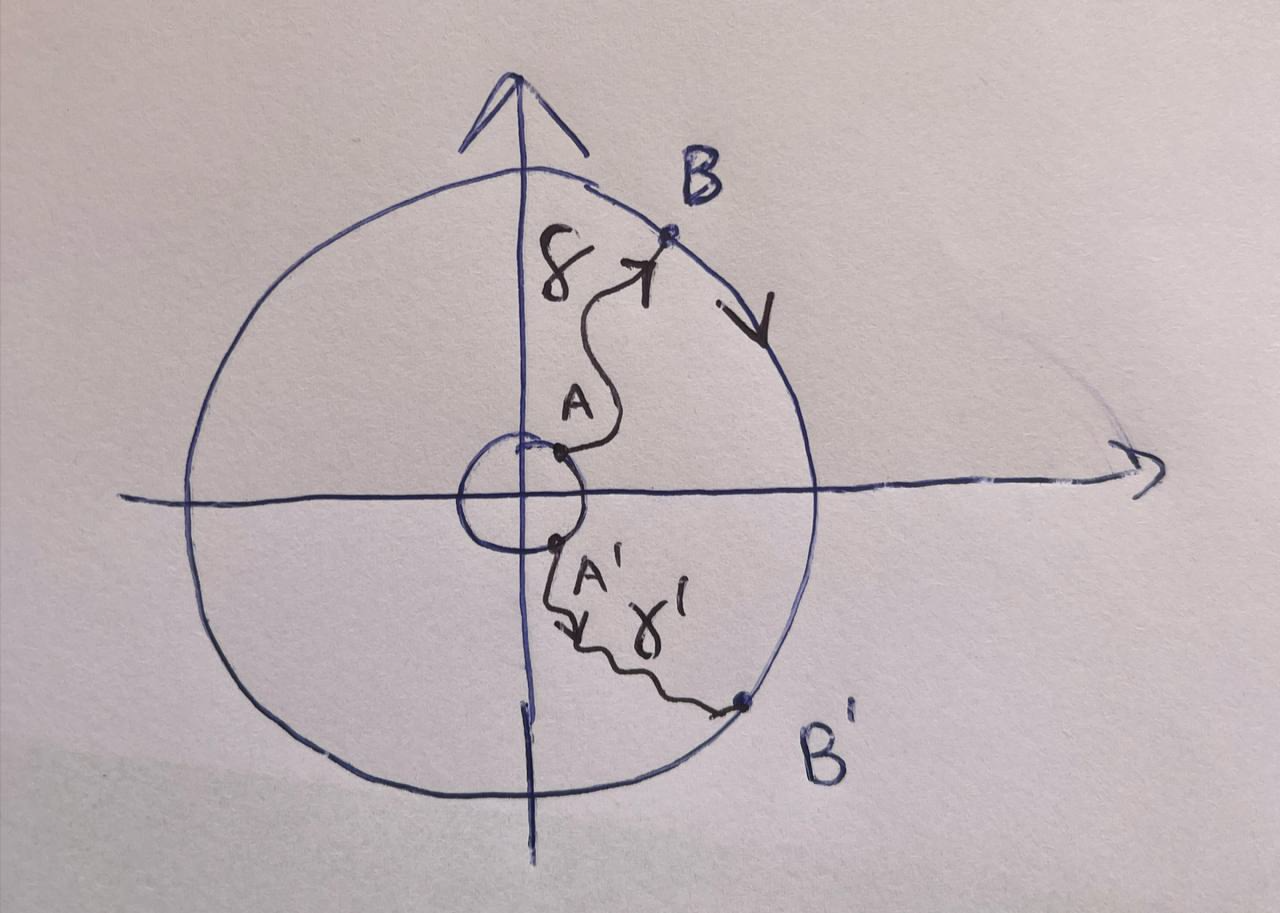
\includegraphics[width=0.5\linewidth]{img/Chapter_three/Chapter3img11.png}
        \end{figure} \\
        La curva è orientata in senso orario. Scriviamo la circuitazione di $\underline{E}$ come:
        \begin{equation}
        \oint_{\mathcal{C}} \underline{E} \cdot \underline{i}_{l}dl = \int_{A} ^{B}  \underline{E} \cdot \underline{i}_{l}dl + 
        \int_{B} ^{B'}  \underline{E} \cdot \underline{i}_{l}dl + (-) \int_{B'} ^{A}  \underline{E} \cdot \underline{i}_{l}dl + \int_{A} ^{A'}  \underline{E} \cdot \underline{i}_{l}dl = 0
        \end{equation}
        dove c'è il meno davanti al terzo integrale perché la curva $\gamma'$ è orientata in modo opposta a $\mathcal{C}$.
        Gli integrali lungo $AA'$ e $BB'$ sono fatti rispettivamente lungo l'anima e la calza, che sono CEP, per cui danno contributo nullo. Allora risulta
        \begin{equation}
        \int_{A} ^{B} \underline{E} \cdot \underline{i}_{l} dl = \int_{A'} ^{B'}  \underline{E} \cdot \underline{i}_{l}dl
        \end{equation}
        e cioè che la circuitazione di $\underline{E}$ tra due punti sui conduttori del cavo è indipendente dalla scelta di questi ultimi. \\
        Resta da determinare se sia possibile, fissato $z$, identificare $\mathcal{V}$ con $V(z)$, dunque scriviamone l'espressione per intero
        \begin{equation}
        \mathcal{V}(z) = \int_{A} ^{B} \underline{E} \cdot \underline{i}_{l}dl = \int_{A} ^{B} \underline{E}_{t} \cdot \underline{i}_{l} dl = \int_{A} ^{B} V(z)\underline{e} \cdot \underline{i}_{l} dl 
        \end{equation}
        Poiché $z$ è fissato, $V(z)$ è un semplice numero
        \begin{equation}
        \implies \mathcal{V}(z) = V(z) \int_{A} ^{B} \underline{e} \cdot \underline{i}_{l} dl
        \end{equation}
        Dobbiamo dimostrare che l'integrale di linea di $\underline{e}$ faccia uno. Esprimendolo come
        \begin{equation}
        \int_{A} ^{B} - \nabla_{t} \varphi \cdot \underline{i}_{l} dl = - \int_{A} ^{B} \frac{d \varphi}{d l} dl = \int_{A} ^{B} d \varphi = \varphi(A)-\varphi(B) = 1
        \end{equation}
        Dunque $\mathcal{V}(z) = V(z)$. \newpage 
        \begin{figure}[h!]
        \center  
        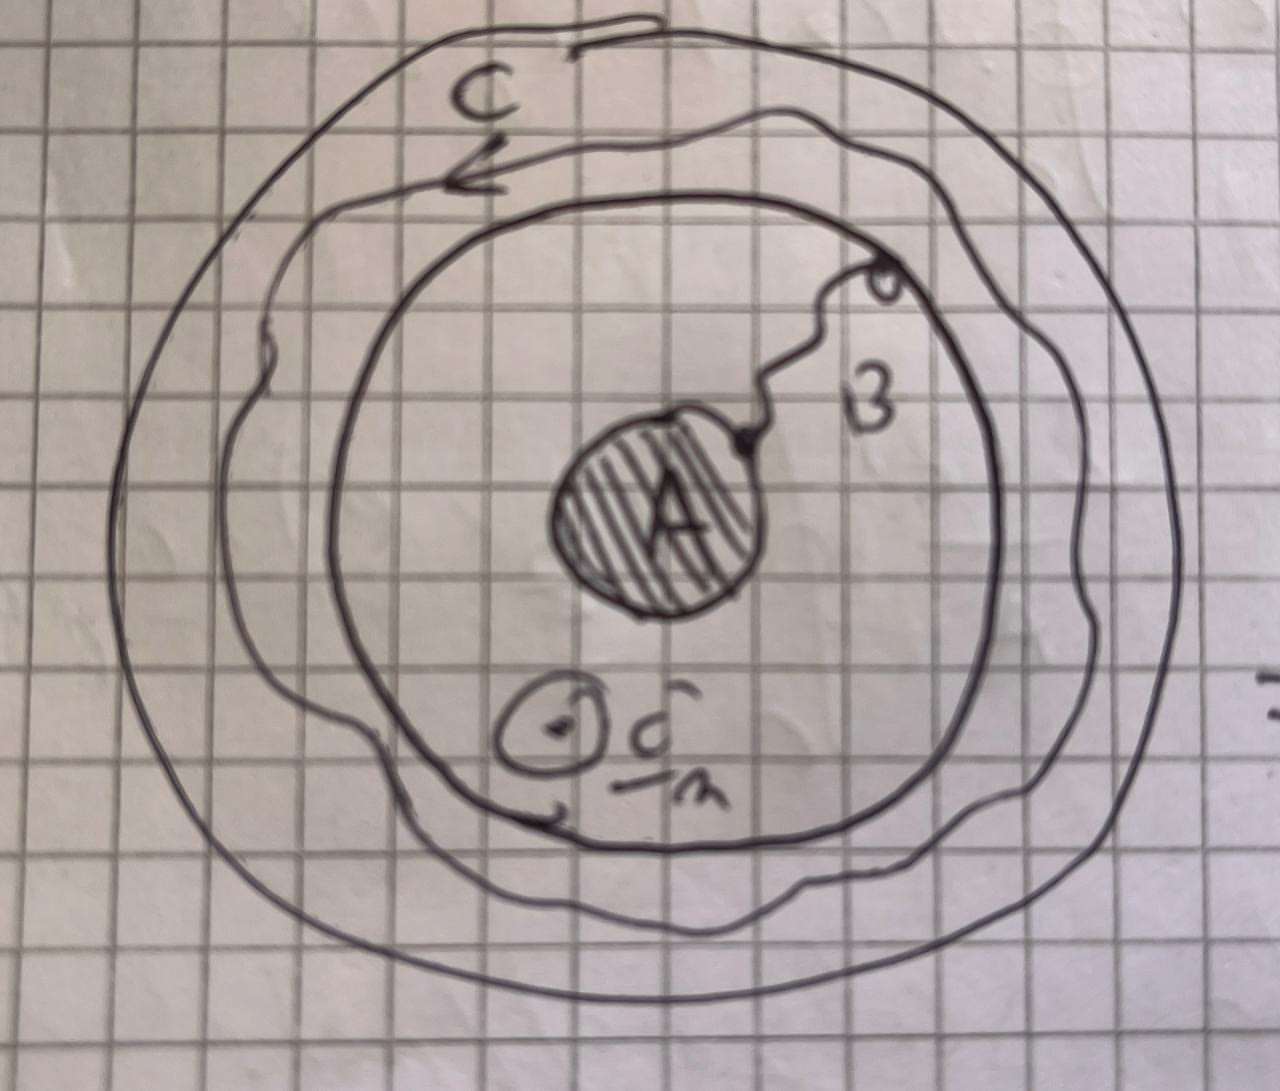
\includegraphics[width=0.6\linewidth]{img/Chapter_three/Chapter3img12.png}
        \end{figure}
        Trattiamo ora la corrente. Ci si aspetta che la corrente sia pari in modulo sulle pareti della calza e dell'anima, ma abbia verso opposto.
        Questo perché all'interno del CEP il campo magnetico è nullo, quindi non c'è corrente netta che scorre nella zona tra l'anima e la calza.
        Noi scegliamo di ricavare l'espressione della corrente che scorre sull'anima, ma è indifferente. Considerata una curva $\mathcal{C}$ all'interno
        della corona circolare, la quale racchiude una superficie $S_{C}$. La circuitazione del campo magnetico è 
        \begin{equation}
        \oint_{\mathcal{C}} \underline{H} \cdot \underline{i}_{l} dl = \underline{i}(\underline{S}_{C}) = \mathcal{I}(z)
        \end{equation}
        in quanto $E_{z} = 0$. Dunque scorre una corrente $\mathcal{I}(z)$ lungo la direzione $z$. Come prima, esprimiamo il campo 
        magnetico (di cui è non nulla solo la componente trasversa) come fattorizzazione fra funzione scalare e vettoriale di modo, 
        fissando $z$:
        \begin{equation}
        \mathcal{I}(z) = \oint_{\mathcal{C}} I(z) \underline{h} \cdot \underline{i}_{l}dl = I(z) \oint_{\mathcal{C}} \underline{h} \cdot \underline{i}_{l} dl= \frac{I(z)}{A}\oint_{\mathcal{C}} (\underline{i}_{z} \times \underline{e}) \cdot \underline{i}_{l}dl
        \end{equation} 
        È arrivato il momento di scegliere $A$ in modo tale $I(z) = \mathcal{I}(z)$. Notiamo dapprima che  in coordinate
        polari $\underline{i}_{l} = \underline{i}_{\vartheta}$, che è uno dei versori del sistema di riferimento polare. Inoltre,
        $\underline{i}_{\vartheta} \times \underline{i}_{z} = \underline{i}_{\rho}$, che è l'altro versore nel piano polare. Per cui possiamo manipolare 
        l'espressione come segue
        \begin{equation}
        \implies \frac{1}{A} \oint_{\mathcal{C}} \underline{i}_{z} \times \underline{e} \cdot \underline{i}_{\vartheta} dl =
        \frac{1}{A} \oint_{\mathcal{C}} \underline{i}_{\vartheta} \times \underline{i}_{z} \cdot \underline{e} dl 
        \end{equation} 
        \begin{equation}
        \implies \frac{1}{A} \oint_{\mathcal{C}} \underline{i}_{\rho} \cdot \underline{e} dl = - \frac{1}{A} \oint_{\mathcal{C}} \underline{i}_{\rho} \nabla_{t} \varphi dl
        = - \frac{1}{A} \oint_{\mathcal{C}} \frac{d \varphi}{d\rho} dl
        \end{equation}
        avendo sfruttato la derivata direzionale. Poiché: 
        \begin{equation}
            \varphi(\rho) = c_{1} \ln(\rho) = \frac{1}{\ln(\frac{a}{b})}\frac{1}{\rho} \implies \frac{d \varphi}{d \rho} = \frac{1}{\ln(\frac{a}{b})}\frac{1}{\rho}
        \end{equation}
        \begin{equation}
            \implies \mathcal{I}(z) = -\frac{1}{A} \oint_{\mathcal{C}} \frac{1}{\ln(\frac{a}{b})}\frac{1}{\rho} dl        \end{equation}
        L'unico termine che dipende da $l$ è $dl$ che integrato sulla circonferenza fa $2\pi$, per cui
        \begin{equation}
            \mathcal{I}(z) = I(z) \frac{1}{A} \frac{2 \pi \rho}{\ln(\frac{b}{a}) \rho} \frac{1}{A} \implies A = \frac{2\pi}{\ln(\frac{b}{a})}
        \end{equation}
        Si faccia sempre attenzione che per togliere il segno meno si è sfruttato $-\ln(a/b) = ln(b/a)$!. Dunque per un modo TEM la funzione scalare di modo 
        per il campo magnetico è proprio la corrente. \\
        Come avevamo già anticipato nel capitolo sulle linee di trasmissione, il fattore geometrico determina l'impedenza 
        caratteristica della linea 
        \begin{equation}
            Z_{0} = \frac{\zeta}{A} = \frac{\zeta}{2 \pi} \ln (\frac{b}{a}) \qquad \zeta = \frac{\mu}{c}
        \end{equation}
        \section{Potenziali elettromagnetici}
            I potenziali elettromagnetici sono grandezze ausiliari utili per risolvere le equazioni di Maxwell. Supponiamo di avere una sorgente di campo $(\underline{J}_{0}, \rho_{0})$. Per l'equazione di
            continuità
            \begin{equation}
                \nabla \cdot \underline{J}_{0}+ j \omega \rho_{0} = 0
            \end{equation}
            Trattiamo il problema all'interno di un volume limitato $V$, cioè tale da poter essere contenuto in una sfera di raggio sufficientemente grande. Supponiamo inoltre che il mezzo sia normale e omogeneo
            nello spazio. Le equazioni di Markuvitz-Schwinger assumono la forma
            \begin{equation}
                \begin{cases}
                    \displaystyle \nabla \times \underline{E} = -j \omega \mu \underline{H} \\
                    \displaystyle \nabla \times \underline{H} = j \omega \varepsilon \underline{E}+\underline{J}_{0} \\
                    \nabla \cdot (\varepsilon \underline{E}) = \rho \\
                    \nabla (\mu \underline{H}) = 0
                \end{cases}
            \end{equation}
            Il campo $\underline{B}= \mu \underline{H}$ è indivergente. Se supponiamo che il dominio sia a connessione superficiale semplice\footnote{cioè tale per cui è possibile deformare una superficie in un punto senza uscire dal dominio}
            il campo è \textbf{solenoidale}, per cui è possibile definire un \textbf{potenziale vettore} $\underline{A}$ tale per cui
            \begin{equation}
                \mu \underline{H} = \nabla \times \underline{A}
            \end{equation}
            Il dominio $\mathbb{R} ^{3}$ nel quale stiamo cercando la soluzione è a connessione superficiale semplice, dunque $\underline{B}$ è sicuramente solenoidale.
            Sostituendo il tutto nella IV equazione di MS\footnote{Markuvitz-Schwinger ndr.}:
            \begin{equation}
                \nabla (\mu \underline{H}) = \nabla \cdot \nabla \times \underline{A} = 0 \implies \nabla \times \underline{A} = 0
            \end{equation}
            Dunque $\underline{A}$ è irrotazionale. Se sostituiamo nella I equazione di MS
            \begin{equation}
                \implies \nabla \times \underline{E} + j \omega \nabla \times A = 0 \implies \nabla \times (\underline{E}+j \omega \underline{A}) = 0
            \end{equation}
            Dunque il campo $\underline{E}+j\omega A$ è irrotazionale. Se il dominio è a connessione lineare semplice, il campo è, in quanto irrotazionale, conservativo. Poiché $\mathbb{R} ^{3}$ è sia a connessione
            lineare che superficiale semplice, il campo è conservativo, per cui esiste una funzione scalare $\varphi$, che prende il nome di \textbf{potenziale scalare}, tale per cui
            \begin{equation}
                \underline{E}+j \omega \underline{A} = - \nabla \varphi
            \end{equation} \\ \\
            Occorre allora determinare $\underline{A}$ e $\varphi$ e lo si può fare sfruttando le altre due equazioni che ci restano. Per la seconda equazione si ottiene:
            \begin{equation}
                \underline{H} = \frac{1}{\mu} \nabla \times \underline{A} \implies \nabla \times (\frac{1}{\mu} \nabla \times \underline{A}) = j \omega \varepsilon \underline{E}+\underline{J}_{0} 
            \end{equation}
            \begin{equation}
                \implies \underline{H} = j \omega \underline{E}(-j \omega \underline{A}- \nabla \varphi)+\underline{J}_{0}
            \end{equation}
            Aggiungendo e sottraendo $k^{2} = -j^{2} \omega ^{2} \mu \varepsilon$
            \begin{equation}
                \nabla ^{2} \varphi + k ^{2} \varphi = -j^{2} \omega ^{2} \mu \varepsilon - \frac{\rho}{\varepsilon}-j \omega \nabla \cdot \underline{A}
            \end{equation}
            \begin{equation}
                = - \frac{\rho}{\varepsilon}-j\omega (j \omega \mu \varepsilon + \nabla \cdot \underline{A})= \nabla ^{2} \varphi+k ^{2} \varphi
            \end{equation}
            In definitiva, occorre risolvere il seguente sistema
            \begin{equation}
                \begin{cases}
                    \underline{H} = \frac{1}{\mu} \nabla \times \underline{A} \\
                    \underline{E} = -j \omega \underline{A}-\nabla \varphi \\
                    \nabla ^{2} \underline{A}+k^{2}\underline{A}= \nabla(\nabla \cdot \underline{A}+j \omega \varepsilon \mu \varphi)+\underline{J}_{0} \\
                    \displaystyle \nabla ^{2} \varphi +k^{2} \varphi = -\frac{\rho}{\varepsilon}-j \omega ( \nabla \cdot \underline{A}+j \omega \varepsilon \mu \varphi)
                \end{cases}
            \end{equation}
            Ci sono meno incognite rispetto alle equazioni di Maxwell, ma il problema ora è alle derivate del secondo ordine (Maxwell era al primo). Inoltre, le ultime due equazioni sono accoppiate.
            Ci chiediamo allora se esista una coppia di poteniali $\underline{A} '$ e $\varphi '$ tali per cui le due equazioni risultano disaccoppiate, cosa che accade se è soddisfatta
            \begin{equation}
                \nabla \cdot \underline{A} ' +j \omega \varepsilon \mu \varphi ' = 0
            \end{equation}
            detta \textbf{gauge di Lorentz}. \\
            Il campo $\underline{A}$ è definito a meno di un campo irrotazionale $\nabla \psi$, dunque il campo $\underline{A}'$ sarà del tipo
            \begin{equation}
                \underline{A}' = \underline{A}+\nabla \psi \qquad \nabla \times \underline{A} = \nabla \times \underline{A'}
            \end{equation}
            In pratica, $\underline{A}$ ed $\underline{A'}$ generano gli stessi campi. Scriviamo allora 
            \begin{equation}
                \underline{E'}= -j \omega \underline{A'} - \nabla \varphi' = \underline{E}= -j \omega \underline{A} - \nabla \varphi
            \end{equation}
            Per cui, sostituendo l'espressione di $\underline{A'}$
            \begin{equation}
                \underline{E'} = -j \omega \underline{A}-j \omega \nabla \psi - \nabla \varphi ' = -j \omega \underline{A}-\nabla \varphi
            \end{equation}
            \begin{equation}
                \implies \nabla (\varphi - \varphi ') = j \omega \nabla \psi 
            \end{equation}
            Ricapitolando, se valgono le seguenti, il campo elettromagnetico generato dalle coppie di potenziali è lo stesso
            \begin{equation}
                \begin{cases}
                \nabla \cdot \underline{A'}+j \omega \varepsilon \mu \varphi ' = 0 \\
                \nabla (\varphi - \varphi ') = j \omega \nabla \psi \\
                \underline{A'} = \underline{A} +\nabla \psi  
                \end{cases}
            \end{equation}
            Notiamo che la seconda equazione da la seguente informazione:
            \begin{equation}
                \varphi - \varphi ' -j\omega \psi = \textrm{const} = 0 \implies \varphi = \varphi ' + j \omega \psi
            \end{equation}
            che abbiamo potuto porre a zero perché la condizione è sul gradiente. \\
            Sostituiamo ora $\underline{A'}$ e $\psi '$ nella gauge di Lorentz (qui c'è un errore di calcolo oppure è sbagliata l'espressione scritta sopra questa nota, chiedere in classe)
            \begin{equation}
            \nabla \cdot \underline{A'}+j \omega \varepsilon \mu \psi ' = 0
            \end{equation}
            \begin{equation}
                \implies \nabla \cdot \underline{A} + \nabla ^{2}\psi + j \omega \varepsilon (\varphi - j \omega \varepsilon \mu \omega \psi) = 0
            \end{equation}
            \begin{equation}
                \implies \nabla \cdot \underline{A'} + j \omega \varepsilon \varphi + \nabla ^{2} \psi + k^{2} \psi = 0
            \end{equation}
            Posto $\chi = \nabla \cdot \underline{A}+j \omega \varepsilon \psi$ la condizione che deve soddisfare la coppia $\underline{A}$ e $\underline{\psi}$ è
            \begin{equation}
                \nabla ^{2} \psi + k^{2} \psi = - \chi     
            \end{equation}
            detta \textbf{equazione di Helmholtz}.


\chapter{Propagazione libera}
    \section{Polarizzazione}
        Un generico vettore nel dominio del tempo ha la forma
        \begin{equation}
            \underline{v}(\underline{r}, t) = v_{x} (\underline{r},t)\underline{i}_{x}+\underline{v}_{y}(\underline{r},t)\underline{i}_{t}+\underline{v}_{z}(\underline{r}, t) \underline{i}_{z}
        \end{equation}
        Nel dominio dei fasori, fissato $\underline{r}$, ogni componente ha la forma 
        \begin{equation}
            v_{i}(t) V_{0i}\cos(\omega t + \varphi_{i}) \iff V_{0i}e^{j \varphi_{i}} \qquad \i \in \{x, y, z\}
        \end{equation}
        per cui il vettore nel domino della frequenza è 
        \begin{equation}
            \underline{V} = \underline{V}_{r}+\underline{V}_{I} = V_{x}\underline{i}_{x}+V_{y}\underline{i}_{y}+V_{z}\underline{i}_{z} \in \mathbb{C} ^{3}
        \end{equation} \\
        Vogliamo dimostrare che la curva chiusa descritta nel tempo dal vettore $v(t)$ è piana\footnote{cioè si muove giacendo sullo stesso piano}
        \begin{equation}
            \underline{v}(t) = \Re[\underline{V}_{R}+j\underline{V}_{I}] = \Re[(\underline{V}_{R}+j\underline{V}_{I})(\cos(\omega_{0}t)+j\sin(\omega_{0}t))]
        \end{equation}
        \begin{equation}
            = \underline{V}_{R}\cos(\omega_{0}t)-\underline{V}_{I}\sin(\omega_{0}t)
        \end{equation}
        Il vettore $v(t)$, fissato $t$, è combinazione lineare dei vettori parte reale e parte immaginaria della sua trasformata, i quali generano
        quello che viene chiamato \textbf{piano di polarizzazione}. Scelto $z$ ortogonale al piano di polarizzazione e posto $z=0$ in corrispondenza del piano,
        la componente $v_{z}=0$, per cui si può scrivere 
        \begin{equation}
            \begin{cases}
            v_{x}(t) = V_{0x}\cos(\omega_{0}t+\varphi_{x}) \\
            v_{y}(t)=V_{0y}\cos(\omega_{0}t+\varphi_{y})
            \end{cases}
        \end{equation}
        Semplifichiamo ancora di più e scegliamo un riferimento temporale per il quale la fase $\varphi_{x}$ si annulla
        \begin{equation}
            t' = t-t_{0} \implies t =t'+t_{0} \implies \omega t_{0} = - \varphi_{x} \implies t_{0} = -\frac{\varphi_{x}}{\omega_{0}}
        \end{equation}
        In tal modo, sostituendo $t=t'+t_{0}$ e $t_{0}=-\varphi_{x}/\omega_{0}$
        \begin{equation}
            \begin{cases}
            v_{x}(t) = V_{0x}\cos(\omega_{0}t') \\
            v_{y}(t)=V_{0y}\cos(\omega_{0}t+\varphi_{y}-\varphi_{x})
            \end{cases}
        \end{equation}
        La quantità $\Delta \varphi = \varphi_{y}-\varphi_{x}$ è la differenza di fase fra $v_{x}$ e $v_{y}$. Per comodità di trattazione,
        poniamo $t=t'$ e otteniamo
        \begin{equation}
            \begin{cases}
                v_{x}(t) = V_{0x}\cos(\omega_{0}t) \\
                v_{y}(t) = V_{0y}\cos(\omega_{0}t + \Delta \varphi)
            \end{cases}
        \end{equation}
        la quale è una curva parametrica in $t$. Vista così, però, è difficile da trattare.
        Supponiamo che $V_{0x}, V_{0y} \neq 0$. Allora
        \begin{equation}
            \label{eqn:mi_serve7}
            \frac{v_{x}}{V_{0x}} = \cos(\omega_{0}t) \qquad \frac{v_{y}}{V_{0y}} = \cos(\omega_{0}t+\Delta \varphi)
        \end{equation}
        Aggiustiamo il termine nello slot a destra
        \begin{equation}
            \frac{v_{y}}{V_{0y}}= \cos(omega_{0}t)\cos(\Delta \varphi)-\sin(\omega_{0}t)\sin(\Delta \varphi)
        \end{equation}
        \begin{equation}
            \implies [\frac{v_{y}}{V_{0y}} - \cos^{2}(\omega_{0}t)\cos(\Delta \varphi)]^{2}=\sin^{2}(\omega_{0}t)+\sin^{2}(\Delta \varphi)
        \end{equation}
        \begin{equation}
            \stackrel{\sin^{2}+\cos^{2}=1}{\implies} (\frac{v_{y}}{V_{0y}})^{2}+\cos^{2}(\omega_{0}t)\cos(\Delta \varphi)-2\frac{v_{y}}{V_{0y}}\cos(\omega_{0}t)\cos(\Delta \varphi) = sin^{2}(\Delta \varphi)-\cos^{2}(\omega_{0}t)\sin^{2}(\Delta \varphi)
        \end{equation}
        Sostituendo le (\ref{eqn:mi_serve7}) otteniamo, riordinando l'espressione
        \begin{equation}
            \implies (\frac{v_{x}}{V_{0y}})^{2}+(\frac{v_{x}}{V_{0y}})^{2}-2\frac{v_{x}}{V_{0x}}\frac{v_{y}}{V_{0y}}-\cos(\Delta \varphi) = \sin^{2}(\Delta \varphi)
        \end{equation}
        che è l'equazione di un ellisse dall'estremo libero.
\chapter{Esercizi}
    \section{Linee di trasmissione}
        \subsection{Adattamento a singolo stub in serie}
            \begin{figure}[h!]
                \center 
                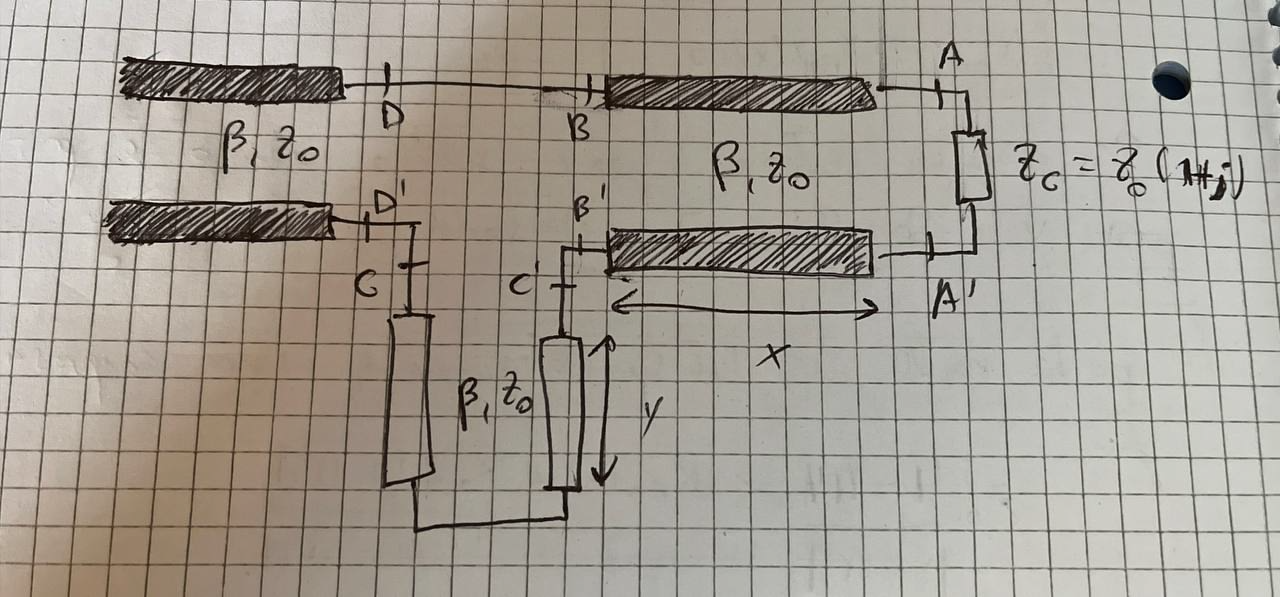
\includegraphics[width=0.75\linewidth]{Chapter_two/Chapt2img21.png}
            \end{figure}
        \textbf{Traccia}: determinare i valori minimi di $x$ ed $y$ affinché $Z_{DD'}=Z_{0}$.
        Partiamo con il calcolo di $Z_{BB'}$ per ottenere la dipendenza da $x$:
        \begin{equation}
            Z_{BB'} = Z_{0} \frac{Z_{C}+jZ_{0}\tan(\beta x)}{Z_{0}+jZ_{C}\tan(\beta x)} =
            Z_{0} \frac{Z_{0}(1+j)+jZ_{0}\tan(\beta x)}{Z_{0}+jZ_{0}(1+j)\tan(\beta x)}
        \end{equation}
        Poniamo, per semplicità di calcolo:
        \begin{equation}
            T_{x}0\tan(\beta x) \qquad T_{y}=\tan(\beta y)
         \end{equation}
         Ottendo dunque:
         \begin{equation}
            Z_{BB'} = Z_{0} \frac{Z_{0}(1+j)+jZ_{0}T_{x}}{Z_{0}+j(1+j)Z_{0}T_{x}} = Z_{0}\frac{1+j(1+T_{x})}{(1-T_{x})+jT_{x}}
         \end{equation}
         Calcoliamone la parte reale:
         \begin{equation}
            R_{BB'} = \Re[Z_{0} \frac{[1+j(1+T_{x})][(1-T_{x}-jT_{x})]}{(1-T_{x})^{2}+T_{x} ^{2}}] = Z_{0}\frac{T_{x} ^{2}+1}{2T_{x} ^{2}-2T_{x}+1}
         \end{equation}
         A questo punto ricaviamo $T_{x}$:
         \begin{equation}
            Z_{0} \frac{1+T_{x} ^{2}}{2T_{x} ^{2}-2T_{x}+1} = Z_{0}
         \end{equation}
         Controlliamo prima se questa relazione ha soluzione all'infinito. Se facciamo tendere $T_{x} \to \infty$ si ottiene:
         \begin{equation}
            \frac{1}{2} = 1
         \end{equation}
         dunque non ha soluzione all'infinito.
         Allora si risolve l'equazione di secondo grado e si ricava:
         \begin{equation}
            T_{x1} = 0 \implies x_{1} = \frac{n \pi}{\beta} \qquad T_{x2} = 2 \implies x_{2} = \frac{\arctan(2)}{\beta}+\frac{n\pi}{\beta}
         \end{equation}
         Per entrambe le soluzioni, $n\geq 0$ affinché si ottengano valori reali. Si noti che se per esempio avessimo ricavato:
         \begin{equation}
            x = -\arctan(2)/\beta +n \pi/\beta
         \end{equation}
         allora $n>1$! Escludendo la soluzione banale per $x=0$, il valore minimo si ottiene per $n=0$ con $x_{2}=arctan(2)$.
         Per semplicità, supponiamo di poter utilizzare $x=0$. A questo punto $T_{x}=0$ e dunque la parte immaginaria di $Z_{BB'}$ sarà semplicemente $Z_{0}$ (basta riutilizzare
         la relazione di sopra). Allora:
         \begin{equation}
            Z_{0}\tan(\beta y) = Z_{0} \implies \beta y = \arctan(1)+n \pi 
         \end{equation}
         ottenendo, come valore minimo $y_{min} = arctan(1)/\beta$.
         Poiché il risultato serve in termini noti, si sostituisce il valore di $\beta = 2\pi /\lambda$, tenendo 
         conto che per un mezzo in aria:
         \begin{equation}
            \lambda = \frac{2\pi f}{c}
         \end{equation}
         dove $f$ è la frequenza di lavoro e $c$ la velocità della luce nel vuoto.
    \newpage
    \subsection*{Equipartizione di potenza a singolo stub}
         Considerato il seguente circuito:
         \begin{figure}[h!]
            \center  
            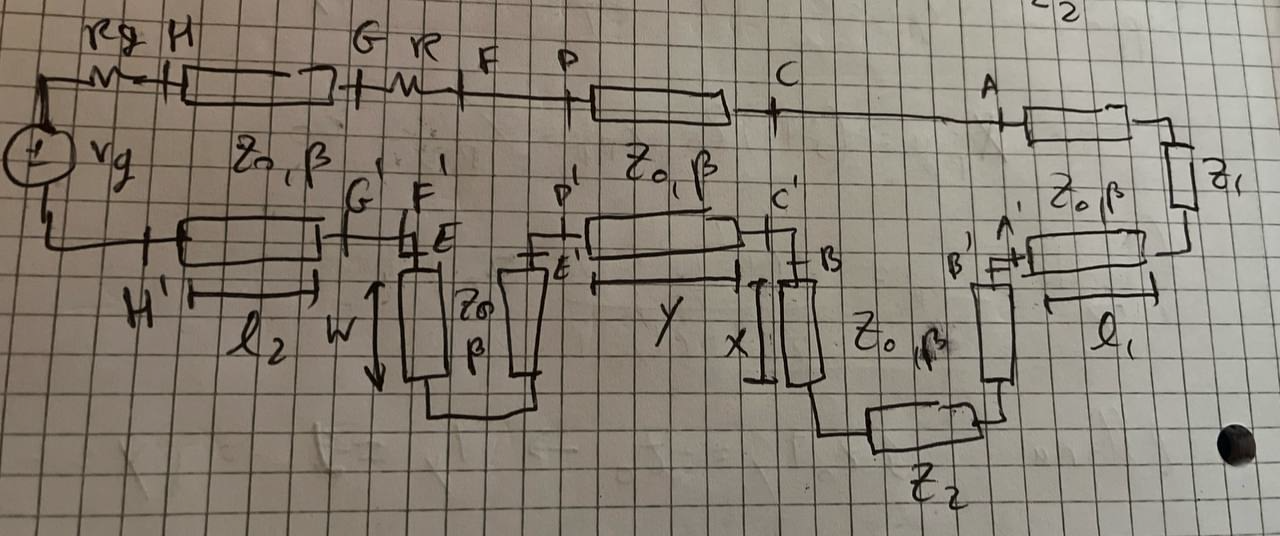
\includegraphics[width=0.8\linewidth]{Chapter_two/Chapt2img22.png}
         \end{figure} \\
         \begin{center}
            \begin{tabular}{c c c c }
                $l_{1} = 0.25m$ & $Z_{0}=50 \Omega$ & $f=150Mhz$ & $R_{g} = 40 \Omega $ \\
                $l_{2}=0.5m$ & $Z_{1}=Z_{0}(1+j)$ & $R=37.5 \Omega$ & $V_{g} = 1V$ \\
                & $Z_{2} = Z_{0}(1+j)$ & &
             \end{tabular}
         \end{center}
         Il mezzo è assunto in aria. Calcolare i valori minimi $x_{min}$ ed $y_{min}$ tali per cui la potenza 
         attiva dissipata su $Z_{1}$  sia la stessa di quella dissipata su $Z_{2}$. \\ \\
         La chiave per risolvere quest'esercizio è tener conto del fatto che, in una linea senza perdite, la potenza attiva si
         conserva, dunque nel nostro caso:
         \begin{equation}
            P_{AA'}=P_{Z_{1}} \qquad P_{BB'}=P_{Z_{2}}
         \end{equation}
         I due carichi sono in serie, dunque la condizione di equipartizione di potenza 
         attiva si riduce all'uguaglianza della parte reale delle impedenza:
         \begin{equation}
            P_{AA'}=\frac{1}{2}R_{AA'}|I_{AA'}|^{2} = P_{BB'} = \frac{1}{2}R_{BB'}|I_{BB'}|^{2} \implies R_{AA'}=R_{BB'}
         \end{equation}
         L'impedenza alla sezione AA' è funzione di termini noti, la calcoliamo immediatamente\footnote{non sviluppando i calcoli per non appensatire il flusso della trattazione}:
         \begin{equation}
            Z_{AA'} = \Re[Z_{0} \frac{Z_{1}\cdot j Z_{0}\tan(\beta l_{1})}{Z_{0}+jZ_{1}\tan(\beta l_{1})}] = Z_{0}\Re[ \frac{1+2j}{j}] = 2Z_{0}
         \end{equation}
         Mentre per la parte reale di $Z_{BB'}$, applicando il trasporto, si ottiene in funzione di $T_{x}=\tan(\beta x)$:
         \begin{equation}
            \Re(Z_{BB'})=Z_{0}\frac{1+T_{x} ^{2}}{2T_{x} ^{2}-2T_{x}+1}
         \end{equation}
         Notiamo subito che non ha soluzione all'infinito, dunque ricaviamo quelle al finito svolgendo l'equazione di secondo grado:
         \begin{equation}
          R_{BB'}=R_{AA'} \implies  Z_{0} \frac{1+T_{x} ^{2}}{2T_{x} ^{2}-2T_{x}+1} = Z_{0} \implies \frac{1+T_{x} ^{2}}{2T_{x} ^{2}-2T_{x}+1} = 1
         \end{equation}
         ed ottenendo come risultati:
         \begin{equation}
            \begin{cases}
                T_{x1}=\frac{1}{3} \\ T_{x2} =1    
            \end{cases} \implies
            \begin{cases}
                x_{1} = \frac{1}{\beta} (\arctan (\frac{1}{3})+n\pi) \\
                x_{2}=\frac{1}{\beta} (\arctan (1)+n\pi) 
            \end{cases}
         \end{equation}
         ottenendo in definitiva il valore di $x$ da sostituire nel calcolo di $Z_{BB'}$:
         \begin{equation}
            x_{min} = \frac{\arctan(\frac{1}{3})}{\beta} \implies Z_{BB'}=Z_{0}(2+j)
         \end{equation}
        \\ La situazione ora è questa qua:
        \begin{figure}[h!]
            \center  
            \includegraphics[width=0.85\linewidth]{img/Esercizi/Esercizi1.png}
        \end{figure} \\
        Il \textbf{secondo punto} chiede di calcolare i valori di $y_{min}$ e $w_{min}$ tali per cui
        $\overline{P}_{Z_{1}}+\overline{P}_{Z_{2}}=\max$ ed i valori delle singole potenze. Dal disegno è immediato verificare che:
        \begin{equation}
            \overline{P}_{Z_{1}}+\overline{P}_{Z_{2}}=\overline{P}_{CC'} =P_{DD'}
        \end{equation}
        e che in virtù dell'equipartizione dell'energia del punto precedente $\overline{P}_{Z_{1}}=\overline{P}_{Z_{2}}$, dunque basta dividere per due 
        la potenza massima per ricavare entrambe. Sullo stub di lunghezza $w$ c'è un carico reattivo, dunque è verificato $\overline{P}_{DD'}=\overline{P}_{FF}$.
        Non possiamo dire lo stesso per la sezione GG', perché c'è un carico resistivo e conseguente dissipazione di potenza attiva:
        \begin{equation}
            P_{GG'}\geq P_{FF'}
        \end{equation}
        In questi casi, conviene applicare Thevenin/Norton per inglobare tutte le cause di dissipazione, così da ricavare la potenza 
        massima erogabile del generatore equivalente, che terrà conto anche delle perdite dovute ai carichi resistivi. In 
        questo caso va applicato Thevenin, perché abbiamo una configurazione serie. Se isoliamo (virtualmente) la sezione FF' dal circuito
        e calcoliamo la $Z_{eq}$ di Thevenin, cioè quella vista da un ipotetico carico in FF' quando il generatore di tensione è cortocircuitato:
        \begin{equation}
            Z_{eq}=Z_{GG'}+R \simeq \frac{Z_{0} ^{2}}{R_{g}}+R = \frac{Z^{2} _{0}}{\displaystyle \frac{4}{5}Z_{0}}+\frac{3}{4}Z_{0}=2Z_{0}
        \end{equation}
        L'approssimazione è giustificata dalla presenza di un tratto a $\lambda/4$, situazione vista in precedenza.
        Per la $V_{eq}$, accendiamo il generatore e apriamo la sezione FF'. La $V_{eq}$ trasportata da HH' (sezione dove c'è il generatore) è 
        \begin{equation}
            V_{eq}=V_{HH'}\cos(\beta \lambda /4)-jZ_{0}I_{HH'}\sin(\beta \lambda /4) = -jZ_{0}I_{HH'} 
        \end{equation}
        Grazie all'aperto a fine sezione, non circola corrente in $R$ per cui:
        \begin{equation}
            V_{eq}=V_{FF'}=-jZ_{0}\frac{V_{g}}{R_{g}+Z_{AA'}} = -jZ_{0}\frac{V_{g}}{R_{g}} = -j\frac{5}{4}V_{g}
        \end{equation}
        perché $Z_{AA'}=0$. Era immediato da fare perché il trasporto di $\lambda/4$ di un aperto è un corto e viceversa, ma almeno
        questo è il procedimento generale. La situazione ora è semplificata di molto:
        \begin{figure}[h!]
            \center  
            \includegraphics[width=0.7\linewidth]{img/Esercizi/Esercizi2.png}
        \end{figure}
        Ora possiamo imporre le condizioni di adattamento fra il generatore equivalente di Thevenin e l'impedenza vista 
        alla sezione FF':
        \begin{equation}
            Z_{FF'}=Z_{eq} ^{*}=2Z_{0} \implies 
            \begin{cases}
                Z_{FF'} = R_{DD'}(y)= 2Z_{0} \\
                X_{FF'} = X_{DD'}(y)+X_{EE'}(w) = 0    
            \end{cases}
        \end{equation}
        A questo punto si applicano i trasporti, si pone $T_{y}=\tan(\beta y), T_{w}=\tan(\beta w)$ e si risolve il sistema:
        \begin{equation}
            \begin{cases}
            R_{DD'} = \Re [Z_{0} \displaystyle \frac{4Z_{0}+jZ_{0}T_{y}}{Z_{0}+j4Z_{0}T_{y}}] =  \displaystyle \frac{4+4T_{y} ^{2}}{1+16T_{y} ^{2}} \\
            X_{DD'}+X_{EE'} = \textrm{Im}[Z_{0} \displaystyle \frac{4Z_{0}+jZ_{0}T_{y}}{Z_{0}+j4Z_{0}T_{y}}] +Z_{0}T_{w} =  \displaystyle -\frac{15T_{y}}{1+16T_{y} ^{2}}+Z_{0}T_{w}
        \end{cases}
        \end{equation}
        ricavando come soluzioni
        \begin{equation}
            T_{y1} = -0.27 \qquad T_{y2}=0.27 \qquad T_{w}=1.87 
        \end{equation}
        \begin{equation}
         \implies \beta y_{1} = -\arctan(0.27)+n\pi \qquad \beta y_{2}=\arctan(0.27)+n \pi \qquad \beta w = \arctan(1.87)+n \pi
        \end{equation}
        \begin{equation}
            \implies y_{min} = \frac{1}{\beta}\arctan(0.27) = 0.084m \qquad w_{min}=0.34m
        \end{equation}
        avendo sostituito $\beta = \displaystyle \frac{2\pi f}{c} = \pi$
        Per il valore numerico della potenza, basta tenere conto che la potenza massima è pari a quella disponibile al \textbf{generatore equivalente} (non a quello originale!):
        \begin{equation}
            \overline{P}_{disp}=\frac{1}{8}\frac{|V_{eq}| ^{2}}{R_{g}} = \frac{1}{8}\frac{|V_{eq} ^{2}|}{2Z_{0}} = 0.125W
        \end{equation}
        \\ \\
        Il \textbf{terzo punto} chiede di calcolare la differenza fra energia elettrica e magnetica media nel tratto di lunghezza $w$.
        In questi casi, dove è richiesta la differenza, si può applicare direttamente il teorema di Poynting alla zona di nostro interesse e risparmiarci
        il calcolo dell'integrale. L'area suddetta è:
        \begin{figure}[h!]
            \center  
            \includegraphics[width=0.7\linewidth]{img/Esercizi/Esercizi3.png}
        \end{figure} \\
        Il flusso del vettore di Poynting attraverso questa superficie $\Sigma$ è dato da:
        \begin{equation}
            \Phi_{\Sigma}(\underline{S}) = \Phi_{\Sigma_{EE'}}+\Phi_{Corto}+\Phi_{Lati}
        \end{equation}
        Ai lati non c'è contributo perché per un CEP il campo elettromagnetico non penetra, mentre il corto non contribuisce
        perché c'è zero campo e dunque zero flusso\footnote{stesso discorso per l'aperto}. In definitiva il flusso dipende unicamente dalla sezione EE'.
        Applicando la relazione di Poynting per la parte immaginaria e tenendo conto che $Phi_{\Sigma} = \Phi_{EE'}$:
        \begin{equation}
            \Phi_{EE'}+2 \omega (\overline{W}_{m}-\overline{W}_{e})=-\textrm{Im}(\frac{j}{2} \iiint_{V} \underline{E} \cdot \underline{J}_{0}dV)
        \end{equation}
        che si riduce, in virtù dell'assenza di sorgenti interne ($\underline{J}_{0}=0)$ a:
        \begin{equation}
            \overline{W}_{m}-\overline{W}_{e} = -\frac{1}{2\omega}\Phi_{EE'}(\underline{S}) = -\frac{1}{2\omega} (-\Im(\frac{1}{2}V_{EE'}I_{EE'} ^{*}))
        \end{equation}
        dove abbiamo messo un meno perché, come sappiamo dalla teoria, la convenzione richiede che il flusso del vettore di Poynting venga calcolato uscente.
        A questo punto ricaviamo tensione o corrente. La corrente che scorre nel corto è la stessa che scorre nel generatore equivalente, dunque:
        \begin{equation}
            I_{EE'} = I_{FF'} = \frac{V_{eq}}{Z_{eq}+Z_{FF'}} = \frac{V_{eq}}{2Z_{eq}} = \frac{V_{eq}}{4Z_{0}}
        \end{equation}
        mentre l'impedenza alla sezione è il trasporto di un corto:
        \begin{equation}
            Z_{EE'}=jZ_{0}\tan(\beta w) \implies \overline{W}_{m}-\overline{W}_{e} = \frac{1}{4 \omega}\frac{1}{2}\textrm{Im}(Z_{EE'}|I_{EE'}|) ^{2}
        \end{equation}
        \begin{equation}
            = \frac{1}{4 \omega} \frac{1}{2}\frac{|V_{eq} |^{2}}{16Z_{0} ^{2}} Z_{0}\tan(\beta w) \simeq 1.65 \cdot 10^{-13}J
        \end{equation}
        \textbf{Il punto quattro} chiede invece la somma dell'energia elettromagnetica alla stessa sezione. Possiamo sfruttare il risultato che già abbiamo sulla differenza 
        e calcolare una fra l'energia magnetica e quella elettrica. Calcoliamo quella elettrica:
        \begin{equation}
            \overline{W}_{e} = \frac{C}{4} \int_{0} ^{w} |V(z)|^{2}dz
        \end{equation}
        dove $C=\displaystyle \frac{\beta}{\omega Z_{0}} = 6.6 \cdot 10^{-11} F/m$ è la capacità per unità di lunghezza della linea.
        A questo punto:
        \begin{equation}
            V(z) = (V_{EE'}\cos(\beta z)-jI_{EE'}Z_{0}\sin(\beta z)) = I_{EE'}(Z_{EE'}\cos(\beta z)-jZ_{0}\sin(\beta z)) 
        \end{equation}
        poiché $Z_{EE'}=X_{EE'}=jZ_{0}\tan(\beta w)$:
        \begin{equation}
            \implies |V(z)| ^{2} = |I_{EE'}| ^{2}|X_{EE'}^{2}\cos^{2}(\beta z)+Z_{0}^{2}\sin^{2}(\beta z)-2X_{EE'}Z_{0}\cos(\beta z)\sin(\beta z)|
        \end{equation}
        A questo punto si risolve l'integrale tenendo conto delle formule di addizione e sottrazione:
        \begin{equation}
            \cos^{2}(x)=\frac{1}{2}(1+\cos(2x)) \qquad sin^{2}(x)=\frac{1}{2}(1-\sin(2x)) \qquad \sin(x)\cos(x)=sin(2x)
        \end{equation}
        Trovato il valore di $W_{e}$ il risultato è facilmente ricavabile con:
        \begin{equation}
            \overline{W}_{e}+\overline{W}_{m}=\overline{W}_{m}-\overline{W}_{e}+2 \overline{W}_{e}
        \end{equation}
        Il \textbf{quinto e ultimo punto} chiede di determinare le distanze $d_{V}$ e $d_{I}$ a partire dal carico dove si ottengono 
        rispettivamente il massimo di tensione ed il massimo di corrente (in modulo). Partiamo dal massimo di tensione, che come sappiamo si può
        esprimere come:
        \begin{equation}
            V(z)=V^{+}(x)(1+\Gamma (z))
        \end{equation}
        poiché la relazione vale a meno di un fattore costante:
        \begin{equation}
            \frac{V(z)}{V^{+}}=1+\Gamma(z) \implies \frac{|V(z)|}{|V^{+}|} = |1+\Gamma (z)|
        \end{equation}
        Si avrà il massimo di tensione per:
        \begin{equation}
            \Gamma (-d_{V}) = \Gamma_{0}e^{-j2 \beta d_{V}} = |\Gamma_{0}|e^{j \varphi_{0}}e^{-j 2 \beta d_{V}}
        \end{equation}
        Calcolando $\Gamma_{0}$ e la relativa fase:
        \begin{equation}
            \Gamma_{0} = \frac{Z_{1}-Z_{0}}{Z_{1}+Z_{0}} = \frac{j}{2+j} \implies 
            \begin{cases}
                |\Gamma_{0}| = \frac{\sqrt{5}}{5} \\ \varphi_{0}=\arctan(2)    
            \end{cases}
        \end{equation}
        si applica il criterio di massimo di tensione visto al capitolo 2\ref{eqn:max_tensione} e si sceglie un valore minore della 
        lunghezza $l_{1}$ della linea, se esiste:
        \begin{equation}
            d_{V}|_{n=0}=\frac{\varphi}{2 \beta} = 0.18m < l_{1}
        \end{equation} 
        Per la corrente il procedimento è identico\ref{eqn:max_corrente}:
        \begin{equation}
            d_{I}|_{n=-1}=\frac{\varphi_{0}-\pi}{2 \beta} = 0.68m>l_{1}
        \end{equation}
        Per la tensione il risultato è maggiore di $l_{1}$, dunque il massimo si trova o all'inizio o alla fine. A questo punto 
        si calcola ambo lati e si sceglie il più piccolo. All'inizio:
        \begin{equation}
            \frac{|I(0)|}{|I^{+}|}=|1-\Gamma_{0}|=\frac{2\sqrt{5}}{5} \simeq 0.89
        \end{equation}
        mentre alla fine:
        \begin{equation}
            \frac{|I_{AA'}|}{|I^{+}|}=|1-\Gamma_{AA'}| \simeq 1
        \end{equation}
        Dunque il massimo sta alla fine.
        \newpage
    \subsection{Stub in parallelo e adattamento $\lambda /4$}
        \begin{figure}[h!]
            \center  
            \includegraphics[width=0.7\linewidth]{img/Esercizi/Esercizi4.png}
        \end{figure}
        \begin{center}
            \begin{tabular}{c c c}
                $f = 100MHz$ & $Z_{0}=50 \Omega$ & $Z_{1}=\frac{3}{2}Z_{0}$ \\
                $l_{1}=0.53m$ & $V_{g}=20V$ & $R_{g}=Z_{0}$
            \end{tabular}
        \end{center}
        
        Il \textbf{primo punto} chiede, assegnato il circuito in figura, i valori $R_{x}$ ed $x_{min}$ tali per cui
        la potenza sul carico $\overline{P}_{R_{x}}=\max$. \\
        Dal disegno, $\overline{P}_{AA'}=\overline{P}_{CC'}$, perché il corto non assorbe alcuna potenza attiva. Per la conservazione 
        della potenza attiva, $\overline{P}_{AA'}=\overline{P}_{R_{x}}$, dunque va massimizzata $\overline{P}_{CC'}$.
        Per fare ciò, tenendo conto che la topologia è in parallelo, facciamo il trasporto di ammettenza alla sezione AA':
        \begin{equation}
            Y_{AA'}=Y_{0}\frac{Z_{0}+jR_{x}\tan(\beta l_{1})}{R_{x}+jZ_{0}\tan(\beta l_{1})} \simeq Y_{0} \frac{Z_{0}+jR_{x}\sqrt{3}}{R_{x}+jZ_{0}\sqrt{3}}
        \end{equation}
        \begin{equation}
            = Y_{0}\frac{4Z_{0}R_{x}+j\sqrt{3}(R_{x} ^{2}-Z_{0} ^{2})}{R_{x} ^{2}+3Z_{0} ^{2}}
        \end{equation}
        mentre $Y_{BB'}$ è immediata:
        \begin{equation}
            Y_{BB'}=jY_{0}T_{x}
        \end{equation}
        avendo posto $T_{x}=\tan(\beta x)$. Arrivati a questo punto si potrebbe pensare di trasportare $Y_{CC'}=Y_{BB'}+Y_{AA'}$ al generatore 
        e adattare, ma è un casino. Quello che conviene fare è utilizzare il teorema di Norton e adattare al generatore di corrente equivalente.
        Applichiamo allora Norton alla sezione CC', ottenendo $Y_{eq}=Y_{0}$. Per l'ammettenza equivalente, c'è il trasporto a $\lambda /4$ dunque si ottiene
        \begin{equation}
            Y_{eq} \simeq (\frac{1}{Z_{1}})^{2}\cdot \frac{1}{Y_{0}} + \frac{1}{Z_{0}} = \frac{(\frac{2}{3}Y_{0})^{2}}{Y_{0}} +Y_{0}= \frac{13}{9}Y_{0} 
        \end{equation}
        Per ora non calcoliamo il generatore equivalente, perché non ci è stato chiesto il valore della potenza ma solo le condizioni per cui 
        è massimo, dunque ci limitiamo ad imporre le condizioni di adattamento al generatore:
        \begin{equation}
            Y_{CC'}=Y_{0}
        \end{equation}
        Nota: da qui in poi inserisco un $4/9$ al posto del $13/9$, perché in classe è venuto questo risultato che però sembra sbagliato, perché
        si ottiene trascurando l'ammettenza del generatore. Non rifaccio i calcoli perché alla fine è il procedimento che conta, ma era doveroso segnalare
        questa cosa. \\
        \begin{equation}
            Y_{CC'} = Y_{0} ^{*} \implies 
            \begin{cases}
                G_{AA'} = \displaystyle \frac{4Y_{0}Z_{0}R_{x}}{R_{x} ^{2}+3Z_{0}} 0 \frac{4}{9}Y_{0} \\
                X_{AA'}+Z_{BB'} = Y_{0} \cdot \displaystyle \frac{\sqrt{3}(R_{x} ^{2}-Z_{0} ^{2})}{R_{x} ^{2}+3Z_{0} ^{2}} +Y_{0}T_{x} = 0
            \end{cases}
        \end{equation}
        Non ci sono soluzioni all'infinito né per $R_{x}$ né per $T_{x}$. Risolviamo allora il sistema in $R_{x}$
        utilizzando la relazione per la parte reale, ottenendo:
        \begin{equation}
            \begin{cases}
                R_{x1} = 8.65\ Z_{0} \\
                R_{x2} = 0.345\ Z_{0}
            \end{cases} \implies \textrm{Scegliamo }R_{x1} = 0.345\ Z_{0} =17.5 \Omega
        \end{equation}
        A questo punto si sostituisce nella seconda equazioni e si ricava il valore di $T_{x}=0.49$, ottenendo 
        il relativo $x_{min}=2.3m$. \\
        Il \textbf{secondo punto} chiede la $V_{g}$ tale per cui $P_{R_{x}}=1W$. Avendo adattato, la potenza dissipata
        su $R_{x}$ è quella disponibile al generatore:
        \begin{equation}
            P_{R_{x}} = \frac{1}{8}\frac{|V_{g}|^{2}}{Z_{0}} = 1W \implies V_{g} = 20V
        \end{equation}
        La \textbf{terza richiesta} è quella di determinare $Z_{1}$ ed $x_{min}$ tale per cui, ipotizzando che $R_{x} = 2Z_{0}$,  $P_{x} = \max$.
        Potremmo adattare come prima, ma sfrutteremo il fatto che possiamo utilizzare il tratto a $\lambda/4$ come adattatore. Abbiamo l'impedenza del 
        generatore è reale, dunque resta da verificare che $Z_{1}$ e $Z_{CC'}$ siano reali.
        Calcoliamo, posto $R_{x}=2Z_{0}$:
        \begin{equation}
            Y_{AA'} = Y_{0} \frac{Z_{0}+j2Z_{0}\tan(\beta l_{1})}{2Z_{0}+jZ_{0}\tan(\beta l_{1})} = Y_{0} \frac{1+2j}{2+j} = Y_{0}\frac{4+j}{5}
        \end{equation}
        \begin{equation}
            \implies Y_{CC'}=Y_{AA'}+Y_{BB'} = (\frac{4}{5}+j\frac{1+T_{x}}{5})Y_{0}
        \end{equation}
        Imponendo che $Z_{CC'}$ sia reale:
        \begin{equation}
            \implies 
            \begin{cases}
                X_{CC'} = \frac{1+T_{x}}{5}Y_{0} = 0 \\
                G_{CC'} = \frac{4}{5}Y_{0}
            \end{cases} \implies T_{x}=-\frac{1}{5} \implies x_{min} =-\frac{\arctan(1/5)}{\beta}+\pi
        \end{equation}
        A questo punto abbiamo la certezza che $Z_{CC'}$ sia reale, dunque $Z_{1}$ applicando la formula dell'adattatore 
        a $\lambda/4$ sarà reale:
        \begin{equation}
            Y_{1} = \sqrt{Y_{0}G_{CC'}} \implies Z_{1} = \frac{1}{\sqrt{Y_{0}G_{CC'}}} = \frac{\sqrt{5}}{2}Z_{0}
        \end{equation}
    La \textbf{quarta richiesta} è l'energia elettrica media nel tratto di lunghezza $x$. Dobbiamo per forza calcolare l'integrale:
    \begin{equation}
        \overline{W}_{e} = \frac{C}{4} \int_{0} ^{x} |V(z)|^{2}dz
    \end{equation}
    con $C=\frac{\beta}{\omega Z_{0}}$. Iniziamo ricavando l'espressione di $V(z)$ tramite la formula del trasporto:
    \begin{equation}
        V(z) = V_{BB'}\cos(\beta z)-jZ_{0}I_{BB'}\sin(\beta z) = V_{BB'}[\cos(\beta z)-j\frac{Z_{0}}{Z_{BB'}}\sin(\beta z)]
    \end{equation}
    \begin{equation}
        =V_{BB'}[\cos(\beta z)-jZ_{0}Y_{BB'}\sin(\beta z)]
    \end{equation}
    con $Y_{BB'}=jY_{0}T_{x}$ (a cui sostituiremo il valore di $T_{x}$ del punto uno). A questo punto, poiché $Y_{0}Z_{0}=1$:
    \begin{equation}
        =V_{BB'}[\cos(\beta z)-jT_{x}\sin(\beta z)]
    \end{equation}
    per cui:
    \begin{equation}
        |V(z)|^{2} = |V_{BB'}|^{2}|\cos^{2}(\beta z)+T_{x} ^{2} \sin ^{2} (\beta z) +2T_{x}\cos(\beta z) \sin(\beta z)|
    \end{equation}
    Svolgendo l'integrale e utilizzando le formule di bisezione:
    \begin{equation}
        \int_{0} ^{x} |V_{BB'}|^{2}|\frac{1}{2}(1+\cos(2\beta z))+T_{x} ^{2} \frac{1}{2}(1-\sin (2\beta z)) +2T_{x}\sin(2\beta z)|dz
    \end{equation}
    \begin{equation}
        =|V_{BB'}| ^{2}[\frac{1}{2}(2z+\frac{1}{2\beta}\sin(2\beta z)+\frac{1}{2\beta}\cos(2\beta z))-\frac{T_{x}}{\beta}\cos(2\beta z)]^{x} _{0}
    \end{equation}
    A questo punto non resta che sostituire i valori nell'integrale. Per ricavare $V_{BB'}=V_{CC'}$ basta applicare il trasporto dal generatore:
    \begin{equation}
        V_{CC'} = V_{g}\cos(\beta \lambda/4)-jI_{g'}Z_{0}\sin(\beta \lambda_{4}) = -jI_{BB'}Z_{0}
    \end{equation}
    Ma la $I_{g'}$ è quella dell'equivalente di Norton:
    \begin{equation}
        I_{g} = \frac{V_{g}}{R_{g}}
    \end{equation}
    dunque viene:
    \begin{equation}
        |V_{BB'}|^{2}=|\frac{V_{g}}{R_{g}}Z_{0}|^{2}
    \end{equation}
    Il \textbf{quinto punto} chiede di calcolare la distanza $d_{I}$ per cui $|I(z)|=\max$. Sappiamo che:
    \begin{equation}
        \frac{|I(d_{I})|}{|I^{+}|} = (1-\Gamma(d_{I}))
    \end{equation}
    Il massimo di corrente lo si ha per:
    \begin{equation}
        \varphi_{0}-2\beta d_{i} = (2n+1)\pi
    \end{equation}
    con $\Gamma(d) =|\Gamma(0)|e^{j\varphi_{0}}e^{j2\beta d}$. Quello che ci serve è $\Gamma(0)$, prendendo come riferimento il carico:
    \begin{equation}
        \Gamma(0) = \frac{R_{x}-Z_{0}}{R_{x}+Z_{0}} = -0.48 \in \mathbb{R} \implies \varphi_{0} = \pi
    \end{equation}
    Scelto $n=-1$ si ottiene:
    \begin{equation}
        d_{I} = \frac{\pi}{2\beta} = \frac{\lambda}{4} = 0.75\textrm{cm}
    \end{equation}
    La linea, però, è lunga solo $l_{1}=0.53\textrm{cm}$! Il massimo si trova allora all'inizio o alla fine.
    In questo caso non c'è bisogno di fare i calcoli per poter affermare che il massimo sta al carico, perché il coefficiente 
    di riflessione è un numero reale negativo, per cui la fase è proprio $\pi$, ragion per la quale si ha il massimo di corrente. Il minimo
    di corrente si troverà, viceversa, alla fine della linea.

    \newpage
    \section{Guide d'onda}
    \subsection*{Primo esercizio guide}
    \begin{figure}[h!]
        \center  
        \includegraphics[width=0.65\linewidth]{img/Esercizi/Esercizi5.png}
    \end{figure}   
    \begin{tabular}{c c c}
        $a = 15\textrm{cm}$ & $b = \frac{a}{2}$ & $f=3GHz$ \\
        $\varepsilon_{1} = 4$ & $\varepsilon_{3}=1$ & $|\underline{E}_{1}|_{max}= 1 \frac{V}{m}$
    \end{tabular}
    Assegnata la guida rettangolare in figura, determinare per il modo fondamentale $TE_{10}$ il valore minimo di $D$ diverso da zero e $\varepsilon_{r2}$ per i quali
    $|\underline{H}_{t}|=\max$ nel tratto tre. Valutare inoltre $|\underline{H}_{3t}|_{x=\frac{a}{4}}$. \\ \\
    Per risolvere questo esercizio bisogna passare alla linea equivalente:
    \begin{figure}[h!]
        \center  
        \includegraphics[width=0.6\linewidth]{img/Esercizi/Esercizi6.png}
    \end{figure} \\
    Occorre calcolare le impedenze caratteristiche e i $k_{z}$ delle sezioni 1 e 3, di cui conosciamo la costante dielettrica relativa. \\
    Per il modo $TE_{10}$ $k_{t_{10}} = \frac{\pi}{a}$, per cui
    \begin{equation}
        k_{z_{i}} = \sqrt{k_{i} ^{2} - k_{t_{10}} ^{2}}= \sqrt{k^{2} - (\frac{\pi}{a})^{2}} \qquad i \in \{1, 2, 3\}
    \end{equation}
    \begin{equation}
        k_{i} = \omega \sqrt{\varepsilon_{0} \mu_{0}} \sqrt{\varepsilon_{i}} = \frac{\omega}{c}\sqrt{\varepsilon_{i}}
    \end{equation}
    Possiamo subito determinare $k_{z1}$ e $k_{z3}$ che risultano:
    \begin{equation}
        k_{z1} = \sqrt{4 \frac{\omega ^{2}}{c ^{2}} - (\frac{\pi}{a})^{2}} = 124 m^{-1} \qquad k_{z3} = 59,3 m^{-1}
    \end{equation}
    le quali sono entrambe reali, quindi le due sezioni sono entrambe in propagazione. Per ricavare le impedenze caratteristiche
    \begin{equation}
        Z_{i} = \frac{\omega \mu_{0}}{k_{z,i}} \implies Z_{1} = 192 \Omega , \ \ \ \ Z_{3} = 400 \Omega
    \end{equation}
    L'onda incidente sulla linea equivalente $V_{1} ^{+}$ va ricavata dall'informazione su $|\underline{E}|_{max} = 1 V/m$. Poiché $\underline{E}_{1} ^{+} = V_{1} ^{+}(z)\underline{e}$
    e per il modo $TE_{10}$ risulta
    \begin{equation}
        \underline{e}_{10} = \underline{e} = -\sqrt{\frac{2}{ab}}\sin(frac{\pi}{a}) \underline{i}_{y}
    \end{equation}
    basta imporre:
    \begin{equation}
        |\underline{E}_{1}|_{max} = \max(|-V_{1} ^{+} \sqrt{\frac{2}{ab}}\sin(\frac{\pi}{a}) \underline{i}_{y}| ) = |V^{+}||\sqrt{\frac{2}{ab}}| = 1 \frac{V}{m}
    \end{equation}
    perché il massimo del seno è uno. Da tale relazione
    \begin{equation}
        |V^{+}| = 0.075V
    \end{equation}
    Poiché
    \begin{equation}
        |H_{t}| = -\sqrt{\frac{2}{ab}}\sin(\frac{\pi}{a}) \underline{i}_{y} \implies |\underline{H}_{3t}|_{x= a/4} = |I_{3} (z)| |\sqrt{\frac{2}{ab}}| |\sin(\frac{\pi}{4})|_{x = a/4} 
    \end{equation}
    \begin{equation}
        = |I_{3} (z)|\frac{1}{\sqrt{ab}}
    \end{equation}
    Dunque occorre massimizzare $|I_{3} (z)| = |I_{AA'} (z)|$, dunque massimizzare la potenza $P_{AA'}$ alla sezione $3$. A questo punto il problema si riduce a quello di un adattamento al generatore.
    \begin{figure}[h!]
        \center  
        \includegraphics[width=0.6\linewidth]{img/Esercizi/Esercizi7.png}
    \end{figure} \\
    Abbiamo fatto l'equivalente di Thevenin per un'indefinita alla sezione $1$ e sostituito il carico $Z_{3}$ alla sezione $3$. Dobbiamo determinare $k_{z2}$ e dunque $Z_{2}$, inoltre carico e impedenza del generatore 
    sono reali, per cui possiamo utilizzare un $\lambda/4$. La lunghezza d'onda da utilizzare è quella del mezzo $2$, per cui si pone
    \begin{equation}
        D = \frac{\lambda_{2}}{4} = \frac{2 \pi}{k_{z2}}
    \end{equation} 
    Poiché vale
    \begin{equation}
        k_{z2} = \sqrt{\varepsilon_{2}(\frac{2 \pi}{\lambda_{0}}) ^{2} - (\frac{\pi}{a})^{2}} \qquad \lambda_{0} = \frac{c}{f}     
    \end{equation}
    occorre determinare $k_{z2}$ e dunque $\varepsilon_{r2}$. Utilizzando la formuala del $\lambda/4$:
    \begin{equation}
        Z_{2} = \sqrt{Z_{1}Z_{3}} = 276,4 \Omega = \frac{\omega \mu_{0}}{k_{z2}} \implies k_{z2} = 85,7 m^{-1}
    \end{equation}
    \begin{equation}
        \implies k_{z2} ^{2} = \varepsilon_{r2} ^{2}(\frac{2\pi}{\lambda_{0}})^{2}-(\frac{\pi}{a})^{2} \implies \varepsilon_{r2} = \sqrt{k_{z2} ^{2} + (\frac{\pi}{a})^{2}} \cdot \frac{\lambda_{0}}{2 \pi} = 1.97
    \end{equation} \\
    \textbf{Il secondo punto} chiede di calcolare l'energia elettromagnetica nel tratto di lunghezza $D$. Applicando Poynting è immediato verificare che $\overline{W}_{e}=\overline{W}_{m}$, perché 
    è un adattatore a $\lambda/4$. Per una guida rettangolare conviene sempre calcolare l'eneria elettrica media, perché il campo elettrico ha solo componente trasversa nel fondamentale $TE_{10}$.
    Per cui
    \begin{equation}
        \overline{W}_{e} = \frac{\varepsilon_{2}}{4} \iiint_{V} |\underline{E}_{t}| ^{2} dV = \frac{\varepsilon_{2}}{4} \int_{0} ^{D} |V_{2}(z)|^{2} dz
    \end{equation}
    perché si dimostra che l'integrale alla sezione trasverale fa $1$ e resta da integrare solo la funzione scalare di modo lungo la componente longitudinale $z$.
    A questo punto si fa nello stesso modo delle linee di trasmissione
    \begin{equation}
        V_{2} = V_{BB'}\cos(k_{z2}z)-jI_{BB'}Z_{2}\sin(k_{z2}z)
    \end{equation}
    per il quale calcolando l'integrale si ricava il valore dell'energia elettrica, e dunque di quella elettromagnetica $W_{em}=2W_{e}$. \\
    \textbf{Il terzo punto} richiede di calcolare $|\underline{H}_{3t}|_{x = \frac{a}{4}}$. Questa richiesta è un semplice problema di bilancio di potenza.
    La componente tangente del campo magnetico dipende dalla corrente alla sezione
    \begin{equation}
        |\underline{H}_{3t}|_{x= \frac{a}{4}} = \frac{1}{\sqrt{ab}} |I_{AA'}|
    \end{equation}
    basta  imporre:
    \begin{equation}
        \overline{P}_{AA'} = \frac{1}{2} Z_{3} |I_{AA'}| ^{2} = P_{disp} \implies |I_{AA'}| = \sqrt{\frac{2P_{AA'}}{Z_{3}}}
    \end{equation}
    Se, ipoteticamente, fosse stato richiesto di massimizzare $H_{3z}$ bastava imporre
    \begin{equation}
        |H_{3z}| = \frac{|V_{3}(z)|}{j \omega \mu_{0}} \frac{\pi}{a} \sqrt{\frac{2}{ab}} |\cos(\frac{\pi}{a}x)|
    \end{equation}
    Poiché nella sezione $3$ c'è solo onda progressiva, si pone $V_{3}(z)=V^{+}$ (cio è vero per una linea indefinita) e si sostituisce $x=a/4$, ripetendo il ragionamento di prima con la tensione. \\ \\
    
    \subsection*{Secondo esercizio sulle guide TBD}
        La struttura guidante di riferimento è la stessa del primo esercizio, con i seguenti dati
    in virtù dell'adattamento al generatore. Per 
\chapter*{Appendice A - Note di carattere matematico}
\section*{Vettori complessi}
        Negli spazi vettoriali definiti su $\mathbb{R}$, è definito il prodotto scalare $(\underline{a}|\underline{b})$ fra $\underline{a}$ e $\underline{b}$ in modo da rispettare le seguenti proprietà:
        \begin{itemize}
            \item $(\underline{a} | \underline{b}) \geq 0$ \\
            \item $(\underline{a}|\underline{a}) = 0 \iff \underline{a} = \underline{0}$ \\
            \item $(\underline{a}|\underline{b}) = (\underline{b}|\underline{a})$
        \end{itemize}
    Nel caso di numeri reali, in sintesi, il prodotto scalare è un marchingegno matematico definito positivo, dal quale si può indurre la norma del vettore $\underline{a}$ in tal modo:
    \begin{equation*}
        ||\underline{a}|| = \sqrt{(\underline{a}|\underline{a})} \implies ||\underline{a}||^{2}=(\underline{a}|\underline{a})
    \end{equation*}
    Geometricamente parlando, il prodotto scalare fra due vettori \textbf{reali} è dato dal prodotto dei moduli per il coseno dell'angolo compreso, che algebricamente è la somma dei prodotti dei singoli componenti:
    \begin{equation*}
        (\underline{a}|\underline{b}) = \sum_{k} a_{k}b_{k}
    \end{equation*}
    Il prodotto scalare definito in questo modo non è adatto per un campo vettoriale complesso. Se per esempio consideriamo $v = 1\underline{i}_{x}+j\underline{i}_{y}$ e applichiamo la definizione di norma indotta dal prodotto scalare per un campo vettoriale reale:
    \begin{equation}
        ||v||^{2} = 1+j^{2}=0
    \end{equation}
    il che è impossibile perché $v \neq 0$. Allora per gli spazi vettoriali definiti sul campo $\mathbb{C}$, ridefiniamo l'operazione analoga del \textbf{prodotto punto} (letto, generando confusione, come "a scalar b"):
    \begin{equation*}
        (\underline{a}|\underline{b}) = \underline{a} \cdot \underline{b}^{*}
    \end{equation*}
    Dunque per il campo complesso il prodotto punto non è commutativo. La commutazione dei due argomenti equivale alla coniugazione del risultato:
    \begin{equation}
        \underline{a} \cdot \underline{b}^{*} = (\underline{b} \cdot\underline{a}^{*})^{*}
    \end{equation}
    \section*{Note sui campi}
        Un campo si dice \textbf{conservativo} se l'integrale di linea percorso da due punti $A$ e $B$
        è invariante rispetto alla curva $\gamma$ che collega $A$ e $B$. È equivalente dire che un campo è conservativo
        se l'integrale di linea lungo qualsiasi curva chiusa è nullo. 
\end{document} 
